\documentclass[10pt,a4paper]{book}
%% \documentclass[10pt,a4paper,landscape]{book}
\usepackage[T1]{fontenc}
\usepackage[latin1]{inputenc}
\usepackage{amsmath}
\usepackage{amsfonts}
\usepackage{amssymb}
\usepackage{makeidx,rotating,graphicx,array}
\usepackage{verbatim,makeidx}
\usepackage{wasysym}
\setcounter{secnumdepth}{4}
\setcounter{tocdepth}{3}
\newcommand{\apiis}{\mbox{\textsc{Apiis} }}
\tolerance=5000

\makeindex
%%\author{Lots of folks }
%%\title{APIIS Developer Documentation}
\begin{document}
\begin{center}
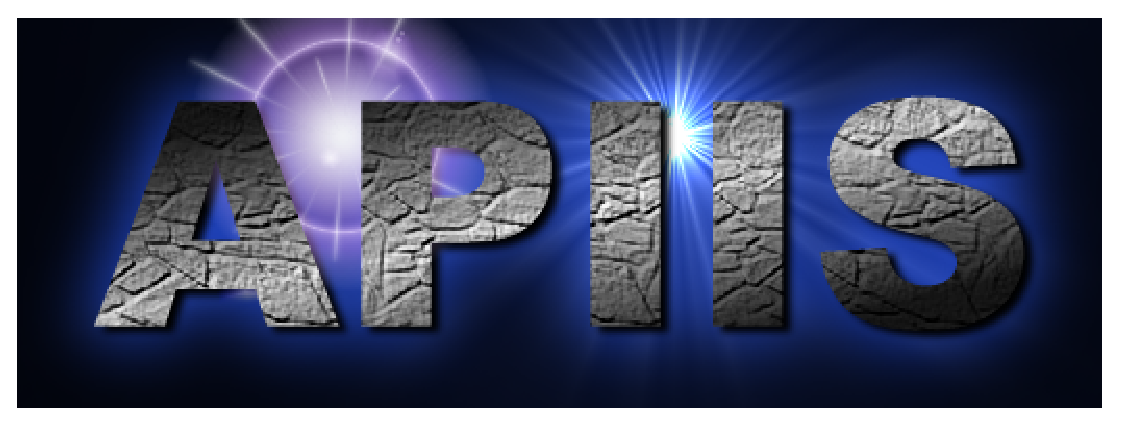
\includegraphics[scale=.7,]{../implementer/apiis6.ps}

\vspace{2cm}
\begin{Huge}\textbf{APIIS Developer Documentation}\end{Huge}
\vspace{1cm}

\begin{Large}\textbf{written by}
\vspace{1cm}

\textbf{Eildert Groeneveld\\
        Zhivko Duchev\\
        Ralf Fischer\\
        Marek Imialek\\
        Helmut Lichtenberg\\
        Detlef Schulze\\}\end{Large}
\vspace{2cm}

 \begin{large}\textbf{Institute of Farm Animal Genetics\\
                      friedrich Loeffler Institute\\
                      Mariensee, Germany\\
                      October 2008}\end{large}
\end{center}
%%\maketitle
%%%%%%%%%%%%%%%%%%%%%%%%%%%%%% Textclass specific LaTeX commands.
 \newenvironment{lyxcode}
    {\begin{list}{}{
     \setlength{\rightmargin}{\leftmargin}
     \listparindent}{0pt}% needed for
                                   AMS classes
     \raggedright
     \setlength{\itemsep}{0pt}
     \setlength{\parsep}{0pt}
     \normalfont\ttfamily}% \item[]}
     {\end{list}}


 \newenvironment{lyxlist}[1]
    {\begin{list}{}
     {\settowidth{\labelwidth}{#1}
     \setlength{\leftmargin}{\labelwidth}
     \addtolength{\leftmargin}{\labelsep}
     \renewcommand{\makelabel}[1]{##1\hfil}}}
     {\end{list}}

 \newcommand{\lyxrightaddress}[1]{
       \par {\raggedleft \begin{tabular}{l}\ignorespaces
          #1
             \end{tabular}
                \vspace{1.4em}
                   \par}
                    }


\tableofcontents
\chapter{Introduction}
In APIIS we define three groups of people working with the system. These
are:
\begin{description}
   \item[developers]the guys (and may be gals) developing the routines
   usually hidden from those people implementing a system
   \item[implementors]people who use the tools box to setup a running
   system, which pertains to a particular set of conditions. This may be
   the cattle population in one country
   \item[users]these are the people who in the end use the system
\end{description}
Clearly, we may sometime find persons who are both implementors and users. 

The developer's documentation covers all software  that is hidden from the
implementors. This means we are talking about the deep and sometimes dark
vaults and sometimes even dungeons of APIIS.

You may be surprised by the section "Undocumented subroutines". Currently,
   the meta layer of APIIS is being rewritten to an object oriented mode. 
   In this process, each routine that is handled will get its own
   documentation section in the Perl code. The subroutines listed here are
   of the non OO kind and will therefore have to converted/replaced by the
   developers. Thus, this chapter serves more like a reminder for them to
   get its length towards zero.

\chapter{The \apiis{} Core}

The \apiis{} core development system provides an object oriented interface to
the basic structures.

Currently these parts build the core:
\begin{itemize}
   \item Basic Initialization
   \item The Model File Interface
   \item The Database Interface
\end{itemize}

\section{Basic Initialization}
% \section{Basic Initialization}

Each program in the \apiis{} suite has to start with the 
preinitialization:

\begin{verbatim}
#!/usr/bin/env perl
##############################################################################
# $Id: basic.tex,v 1.3 2005/03/08 11:02:34 heli Exp $
# Short description about this program
##############################################################################

BEGIN {
   use Env qw( APIIS_HOME );
   die "\n\tAPIIS_HOME is not set!\n\n" unless $APIIS_HOME;
   push @INC, "$APIIS_HOME/lib";
}

use strict;
use warnings;
use Apiis;
Apiis->initialize( VERSION => '$Revision: 1.3 $' );
\end{verbatim}

The \verb+BEGIN+ block checks at compile time, if the environment variable
\verb+$APIIS_HOME+ is set.
\verb+$APIIS_HOME+ is the main starting point for the complete code base of
\apiis. \verb+$APIIS_HOME/lib+ is included into the library search path of
Perl.

\verb+use Apiis.pm;+ loads the \apiis-system into your main namespace and
provides the method initialize().
Usually you should pass the version of your program to \verb+initialize+.
When you commit this program to CVS, the cvs-tag \verb+$Revision: 1.3 $+ will
be replaced by the current version and it will look like
\verb+$Revision: 1.3 $+. You can recall the version later with
\verb+$apiis->version+\index{\verb+$apiis+!\verb+->version+}.
If you don't use cvs then just hardcode the version:
\verb+Apiis->initialize( VERSION => '0.71' );+

Every program which exceeds the intention of being a quick and dirty script for
a small daily job should contain the following two lines before you start coding:

\begin{verbatim}
   use strict;
   use warnings;
\end{verbatim}

You should not ask somebody else to help you track down some bugs in your code unless
you used \verb+strict+ and \verb+warnings+!

\subsection{initialize}\index{initialize}

Besides performing some basic checks the main task of
\verb+initialize+ is the creation of the global
\verb+$apiis+-structure, represented by the object reference \verb+$apiis+.

\subsection{Apiis::Init}
The successfull creation of the \verb+$apiis+ object implies some basic
initializing before and adds various items:
\begin{itemize}
   \item the base configuration from \verb+$APIIS_HOME/apiisrc+
   \item the I18N/L10N part
   \item methods to extend the \verb+$apiis+ structure modularly
   \item methods for logging to files or the system syslog
   \item the public interfaces to set an error status, check this status and
   document errors in detail
   \item handy methods to access the current day and time 
\end{itemize}

The main setup for error handling is done in the package \verb+Apiis::Errors+.

On the main level, the \verb+$apiis+ object provides these public
methods\index{\verb+$apiis+!public methods}:

\smallskip
\begin{tabular}{rl|l}
\verb+$apiis->+& \verb+APIIS_HOME+       & path to \verb+$APIIS_HOME+  \\
               & \verb+APIIS_LOCAL+      & path to \verb+$APIIS_LOCAL+ \\
               & \verb+browser+          & your favourite browser \\
               & \verb+check_status+     & checks the error status \\
               & \verb+code_table+       & usually table 'codes' \\
               & \verb+date_format+      & the date format (US or EU) \\
               & \verb+entry_views+      & hashref of entry-views \\
               & \verb+errors+           & array(reference) of error objects \\
               & \verb+exists_database+  & is the database joined to \verb+$apiis+ \\
               & \verb+exists_form+      & is a form joined to \verb+$apiis+\\
               & \verb+exists_model+     & is the model file joined to \verb+$apiis+ \\
               & \verb+fileselector+     & choose a Tk fileselector \\
               & \verb+HOME+             & path to \verb+$HOME+ \\
               & \verb+join_database+    & join the DataBase object into \verb+$apiis+ \\
               & \verb+join_form+        & join a named Form object into \verb+$apiis+ \\
               & \verb+join_model+       & join the Model object into \verb+$apiis+ \\
               & \verb+language+         & choose user language \\
               & \verb+localtime+        & unformatted timestamp \\
               & \verb+now+              & formatted timestamp \\
               & \verb+programname+      & name of the invoking program \\
               & \verb+reserved_strings+ & reserved strings for data \\
               & \verb+status+           & error status \\
               & \verb+today+            & formatted date \\
               & \verb+user+             & current user \\
               & \verb+version+          & version of the invoking program \\
\end{tabular}

\smallskip
See the POD-documentation for a detailed reference of these methods.

% vim: expandtab:tw=100


\section{The Model File Interface}
%\section{Interfaces to the Model File}

Usually you have to provide the model file\index{Model file}, you
want to use with your \apiis{} program. This is done with
\verb+$apiis->join_model('my_model_file');+.
\verb+join_model()+\index{\verb+$apiis+!\verb+->join_model+} reads in
the model file, parses it and creates public interfaces to all the
information via an object, which is added to the \verb+$apiis+ structure
via \verb+Apiis::Init::_add_object+\index{\verb+$apiis+!\verb+->_add_object+}.
The entry point for these methods is
\verb+$apiis->Model+\index{\verb+$apiis+!\verb+->Model+}.

An auxiliary module to find the model file in the \verb+$APIIS_HOME+
hierarchy is \verb+Apiis::CheckFile+\index{Apiis::CheckFile},
which scans some likely directories for candidates. It also can be used for searching
other configuration files like those for forms or reports.

The model file contains both some basic informations and -- primarily --
the complete database structure\index{database structure}, including business rules.

The basic information can be accessed by these public
methods:\index{\verb+$apiis+!\verb+->Model+!public methods}

\smallskip
\begin{tabular}{rl|l}
\multicolumn{3}{l}{\texttt{\$apiis->Model->}}       \\
                      &\verb+basename+         & basename of the model file \\
                      &\verb+check_level+      & get/set check level \\
                      &\verb+db_driver+        & database driver \\
                      &\verb+db_host+          & database host machine \\
                      &\verb+db_name+          & database name \\
                      &\verb+db_password+      & database password of current user \\
                      &\verb+db_port+          & database system port \\
                      &\verb+db_user+          & database system (meta) user \\
                      &\verb+ext+              & extension of model file name \\
                      &\verb+fullname+         & full name of model file \\
                      &\verb+max_check_level+  & maximum check level reached \\
                      &\verb+path+             & path to model file \\
                      &\verb+table+            & object for detailed table information \\
                      &\verb+tables+           & array(ref) of all tablenames \\
\end{tabular}
\medskip

For all tables in the model file, a table object is created which contains the
information for this table. To get all columns of table 'animal' you could write:

\begin{verbatim}
   my $table_obj = $apiis->Model->table('animal');
   printf "Columns of table animal are: %s\n",
      join(', ', $table_obj->columns);
\end{verbatim}

A more intuitive and shorter way is:

\begin{verbatim}
   printf "Columns of table animal are: %s\n",
      join(', ', $apiis->Model->table('animal')->columns);
\end{verbatim}

The methods of the table object are:\index{\verb+$apiis+!\verb+->Model+!\verb+->table()+!public methods}

\smallskip
\begin{tabular}{rl|l}
\multicolumn{3}{l}{\texttt{\$apiis->Model->table(<name>)->}}       \\
                                     &\verb+check+       & check rules of a column \\
                                     &\verb+cols+        & columns of this table \\
                                     &\verb+columns+     & columns of this table \\
                                     &\verb+datatype+    & meta-datatype of a column \\
                                     &\verb+default+     & default value of a column \\
                                     &\verb+description+ & description of a column \\
                                     &\verb+foreignkey+  & foreign key definition of a column \\
                                     &\verb+index+       & indices for this table \\
                                     &\verb+indexes+     & indices for this table \\
                                     &\verb+indices+     & indices for this table \\
                                     &\verb+length+      & default length of a column (forms) \\
                                     &\verb+modify+      & modify rules of a column \\
                                     &\verb+name+        & name of this table \\
                                     &\verb+primarykey+  & primary key definitions of this table \\
                                     &\verb+rowid+       & get/set rowid of this record \\
                                     &\verb+sequence+    & sequences defined for this table \\
                                     &\verb+sequences+   & sequences defined for this table \\
                                     &\verb+triggers+    & trigger definitions for this table \\
\end{tabular}
\medskip

Most of the mentioned methods will be used rarely as they are implemented in the
newer record object in a more consistent way. Some of them are even outdated, like
the read/write method
\begin{verbatim}
$apiis->Model->table( $mytable )->rowid( $thisrowid );
\end{verbatim}

A future rewrite of the model file interface will have a syntax similar to the record
objects. Instead of 
\begin{verbatim}
$apiis->Model->table($thistable)->foreignkey->($thiscolumn);
\end{verbatim}
it  likely will look like
\begin{verbatim}
$apiis->Model->table($thistable)->column($thiscolumn)->foreignkey;
\end{verbatim}
This will give a a consistent syntax according to this record object example:
\begin{verbatim}
$record_obj->column($thiscolumn)->foreignkey;
\end{verbatim}

% vim: expandtab:tw=100


\section{The Database Interface}
%\section{Interfaces to the Database}

When the Model object is joined into the \verb+$apiis+ structure, by
default the database connection will be configured and initialized. Another
object called DataBase\index{\verb+$apiis+!\verb+->DataBase+}
is integrated into \verb+$apiis+. 

For rare situations you can circumvent this immediate connection to the
database (e.g. if you want to drop the whole database during
initialization) with a special parameter to
\verb+join_model()+\index{\verb+$apiis+!\verb+->join_model+}. See the
POD-documentation of \verb+join_model()+ for details.

The database connections are based on the configuration
parts of the model file and the database specifics, found in
\verb+$APIIS_HOME/lib/<db_driver>.conf+%
\index{\verb+$apiis+!\verb+->DataBase+!driver configuration}.

If no errors occur, a Apiis::DataBase::Init-object will be created and
joined into the \verb+$apiis+ structure as \verb+$apiis->DataBase+.

Two connections to the database will be openend, one for the system
user\index{\verb+$apiis+!\verb+->DataBase+!system user}
with full access to the database and the other as the currently connected
user\index{\verb+$apiis+!\verb+->DataBase+!current user}
with access to the suite of views that reflect his authorization
status.\index{Authorization!views}
These two connections build the base for the public methods
\verb+sys_sql()+\index{\verb+$apiis+!\verb+->DataBase+!\verb+->sys_sql+}
and \verb+user_sql()+\index{\verb+$apiis+!\verb+->DataBase+!\verb+->user_sql+}.

The following public methods are defined with
\verb+$apiis->DataBase+:\index{\verb+$apiis+!\verb+->DataBase+!public methods}

\smallskip
\begin{tabular}{rl|l}
\multicolumn{3}{l}{\texttt{\$apiis->DataBase->}}       \\
                      &\verb+bindtypes+        & database bindtypes \\
                      &\verb+commit+           & commit changes to the database \\
                      &\verb+connect+          & DB-specific connect string for DBI \\
                      &\verb+connected+        & flag if DB is already connected \\
                      &\verb+datatypes+        & datatypes of this DB for our metatypes \\
                      &\verb+dateorder+        & default (?) date order of this DB \\
                      &\verb+datesep+          & date separator \\
                      &\verb+db_has_sequence+  & flag, if this DB has sequences \\
                      &\verb+disconnect+       & method to disconnect from DB \\
                      &\verb+explain+          & explain syntax (curr. not used) \\
                      &\verb+rollback+         & rollback all changes \\
                      &\verb+rowid+            & name of the rowid \\
                      &\verb+seq_next_val+     & method that returns the next sequence value \\
                      &\verb+sequence_call+    & how to call a sequence \\
                      &\verb+sys_dbh+          & database handle for system user \\
                      &\verb+user_dbh+         & database handle for common user \\
\end{tabular}
\medskip


\section{The Database Record Object}
%\section{The Database Record Object}

Still unwritten. \frownie \\
But some POD already exists. \smiley

At least here is the list of the public methods of
\verb+Apiis::DataBase::Record+\index{Apiis::DataBase::Record}:

\smallskip
\begin{tabular}{rl|l}
\multicolumn{3}{l}{\texttt{\$record\_obj->}}       \\
               &\verb+action+               & record action (like insert, update) \\
               &\verb+addcolumn+            & add a column to the record object \\
               &\verb+check_level+          & get/set check level \\
               &\verb+column+               & reference to a column object \\
               &\verb+columns+              & names of all columns \\
               &\verb+decode_column+        & decode on column level \\
               &\verb+decoded+              & decoded flag \\
               &\verb+decode_record+        & decode whole record \\
               &\verb+delcolumn+            & delete a column from the record object \\
               &\verb+delete+               & SQL delete action \\
               &\verb+encode_column+        & encode on column level \\
               &\verb+encoded+              & encoded flag \\
               &\verb+encode_record+        & encode whole record \\
               &\verb+expect_columns+       & which columns are expected by a fetch \\
               &\verb+expect_rows+          & how many records are expected by a fetch \\
               &\verb+fetch+                & SQL fetch/query action \\
               &\verb+fk_table+             & foreign key table \\
               &\verb+indexes+              & indexes of this table \\
               &\verb+insert+               & SQL insert action \\
               &\verb+max_check_level+      & max check level in model file \\
               &\verb+name+                 & (table)name of this record \\
               &\verb+new+                  & create new record object \\
               &\verb+print+                & print record (debug) \\
               &\verb+rows+                 & number of rows returned by SQL action \\
               &\verb+sequences+            & sequences defined in this table \\
               &\verb+tablename+            & name of this table \\
               &\verb+type+                 & type of this record object (database) \\
               &\verb+update+               & SQL update action \\
               &\verb+value+                & value returned by last SQL action \\
               &\verb+values+               & values returned by last SQL action \\
\end{tabular}
\medskip

\subsection{The Column Object}
Besides record level methods, the record object contains one column object for each column of this table. The public
methods to access the columns are:

\smallskip
\begin{tabular}{rl|l}
\multicolumn{3}{l}{\texttt{\$record\_obj->column(<columnname>)->}} \\
         & \verb+check+         & check rules of this column \\
         & \verb+datatype+      & datatype \\
         & \verb+db_column+     & database column name \\
         & \verb+default+       & default value from model file \\
         & \verb+description+   & description for this column \\
         & \verb+extdata+       & external data (array!) \\
         & \verb+foreignkey+    & foreign key definition of this column \\
         & \verb+intdata+       & internal data (scalar) \\
         & \verb+length+        & default length of this column (forms) \\
         & \verb+modify+        & modify rules of this column \\
         & \verb+name+          & name of this column (usually =db\_column) \\
         & \verb+updated+       & updated flag \\
\end{tabular}
\medskip

Example:

\begin{verbatim}
    my ($fk_table, $fk_column, @rest) =
       $record_obj->column( $thiscolumn )->foreignkey;
\end{verbatim}



\chapter{The Meta-layer}

\section{Data-flow schema}
In Apiis both ordinary SQL statements and PseudoSQL  \index{PseudoSQL} statements are allowed. From the standard SQL92 syntax only \'simple\' insert, update and delete can be used. These statements get parsed and  data are filled in  the internal part of record object where the access rights check against the user rights take place. After successfully passing the access rights check the statement is executed via the meta-user account in the database - just like the ordinary PseudoSQL statements.\linebreak
The ordinary Select statements can be very complicated and hard to parse therefore they follow different route - these statements are not parsed, but directly executed via user account  against the views in his own schema. These views are subset of the standard tables restricted with the user access rights, and have the same name as the original table. There the only item in the database that user has access to.
\linebreak The PseudoSQl statements get parsed, loaded in the external part of record object and then encoded, checked against access rights and executed via the meta-user account.
The flow is shown on \ref{fig:meta1} 
\begin{figure}
   \centering
   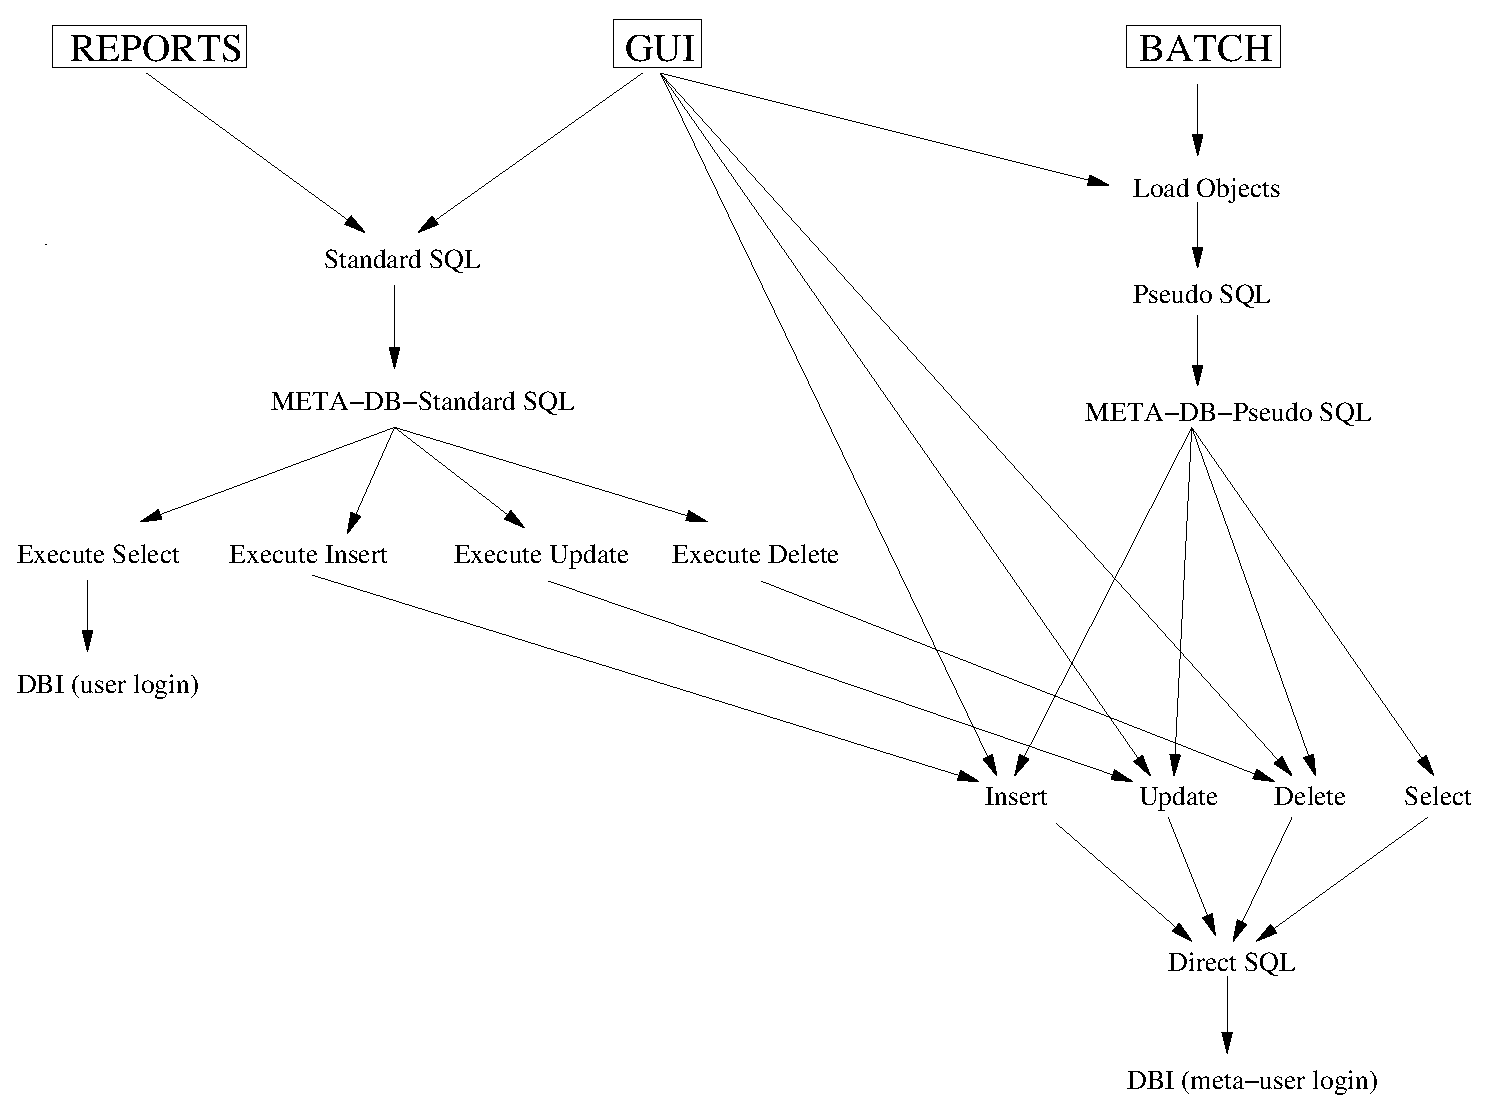
\includegraphics[scale=0.5]{./meta-layer/meta1.eps}
   \caption{}
\label{fig:meta1}
\end{figure}
\begin{figure}
   \centering
   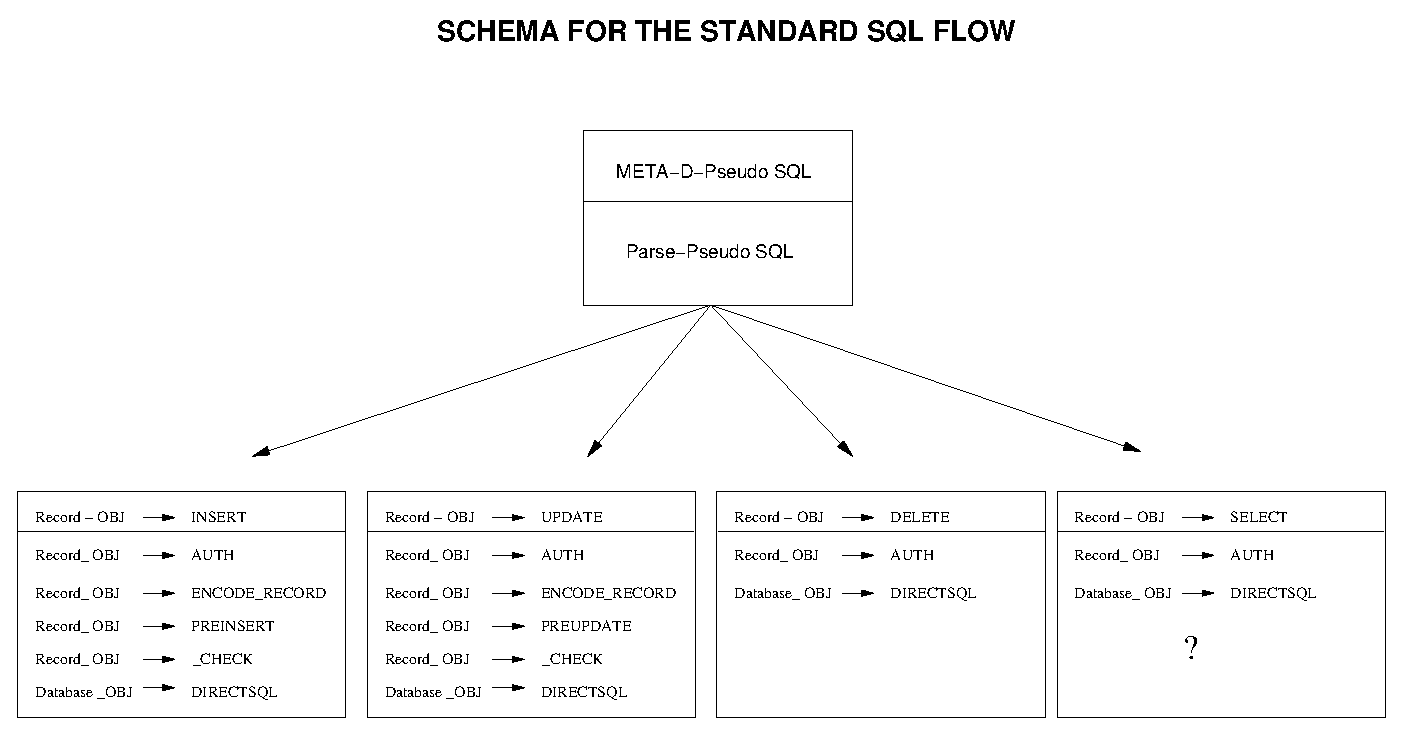
\includegraphics[scale=0.5]{./meta-layer/meta2.eps}
   \caption{}
   \label{fig:meta2}
\end{figure}

 
\section{PseudoSQL language definition}

In this chapter the formal definition of the PseudoSQL language is described.

The PseudoSQL has only INSERT, UPDATE, DELETE and SELECT \index{SELECT} statement.

\begin{verbatim}
 <pseudosql_statement> ::= <insert_statement> |
 			   <update_statement> |
			   <delete_statement> |
			   <select_statement> 
 \end{verbatim}


\subsection{INSERT}
\begin{verbatim}
    <insert_statement> ::= 'INSERT INTO  <table_name>
    				 ( <column_name> {, <column_name> })
                                  VALUES ( <value> {, <value> })'

	 <table_name> ::=>  <identifier> 

	 <identifier> ::= LETTER{LETTER|DIGIT}

	 <column_name> ::= <identifier> 

	 <value> ::= <scalar>|<string>|<variable>|<function> 

	 <scalar> ::= DIGIT{DIGIT}|DIGIT{DIGIT}.DIGIT{DIGIT}

	 <string> ::= ''{LETTER|DIGIT}''

	 <variable> ::= $<hash_key>[<external_fields>]

	 <hash_key> ::= <identifier> 

	 <external_fields> ::=[<field_list>]|[] 
	 here [] means square brackets, not optional element

	 <field_list> ::= ``<hash_key>{,<hash_key>}''

	 <function> ::= concat( <item> , <item> {,item})

	 <item> ::= <value>|<variable>|<string>.<variable>|<variable>.<string> 

\end{verbatim}

\subsection{UPDATE}

\begin{verbatim}


 <update_statement> ::= 'UPDATE  <table_name>
                         SET  <column_name> = <value> {, <column\_name> = <value> }
                         [WHERE  <where_clause> ]'

 <where_clause> ::= <column_name><operator><value>[ <AND|OR> <column_name><operator><value> ]

\end{verbatim}

\subsection{DELETE}

\begin{verbatim}

 <delete_statement> ::= 'DELETE FROM  <table_name>  [WHERE  <where_clause> ]'

\end{verbatim}

\subsection{SELECT}

\begin{verbatim}
 <select_statement> ::= 'SELECT  <variable> {, <variable> }
                         FROM  <table_name>
                         [WHERE  <where_clause> ]'

\end{verbatim}

\section{PseudoSQL flow}

\textbf{Subroutine name:} meta\_db\_PseudoSQL

\textbf{Input:} PseudoSQL - string

\textbf{Output:} 

\textbf{Description:}

\begin{enumerate}
\item Parses the PseudoSQL string using the Parse\_PseudoSQL subroutine
- to be written 
\item Executes the statement by call to a responding record object method:
{}``insert'', {}``update'' or {}``delete'';
\end{enumerate}
\textbf{Subroutine name:} Parse\_PseudoSQL

\textbf{Input:} PseudoSQL - string

\textbf{Output:} Record object filled with the data from the PseudoSQL
string

\textbf{Description: }

\begin{enumerate}
\item Parses the input string - gets the action name, table, column names,
column values and the where clause of the PseudoSQL - to be written 
\item Creates links between LO keys and database columns. These links will be used for targeting the errors, that may come from the underlying levels - to be written
\item Modifies and encodes the where clause and query the database for the
rowid of the first record responding to this where clause - to be
written
\item Creates record(table) object for the table parsed from the string:
my \$thisrecord = Apiis::DataBase::Record-> new( tablename =>  \$table,
); 
\item Fills the columns values from the PseudoSQL statement and the rowid
in the responding column objects using the record object method {}``extdata''
: \$record-> column(\$column\_name)-> extdata(\$column\_value); 
\end{enumerate}

\section{Standard SQL flow}

\textbf{Subroutine name:} meta\_db\_StandardSQL

\textbf{Input:} ordinary SQL - string

\textbf{Output:} 

\textbf{Description:}

\begin{enumerate}
\item Recognizes the sql action and if it is {}``SELECT'' executes it
through the view system using subroutine {}``ExecuteSelect'' 
\item In case of INSERT, UPDATE or DELETE parses the SQL string using the statement object from APIIS/DataBase/SQL/Statement.pm 
\item Calls the responding subroutine: {}``ExecuteInsert'', {}``ExecuteUpdate'' or {}``ExecuteDelete''

\end{enumerate}
\textbf{Subroutine name:} ExecuteSelect

\textbf{Input:} ordinary SQL SELECT statement- string

\textbf{Output:} Statement handle 

\textbf{Description:}

\begin{enumerate}
\item Connects to the database with the user login and executes the Select statement. For each user we will have also a database account and user's own schema(namespace) in the database. This schema will have the same name as the user database login and in this schema all original tables will be masked with views with the same names. For each table we will have a view that is a subset of the original table based on the access rights of the user. The user will have only read access to his schema and no access rights for the rest of the database   - to be written
\end{enumerate}

\textbf{Subroutine name:} ExecuteInsert

\textbf{Input:} parsed sql statement object

\textbf{Output:} 

\textbf{Description: }
\begin{enumerate}
\item Creates record(table) object for the table returned by the statement object; 
\item Fills the columns values from the statement in the responding column objects using the record object method {}``intdata''
\item Executes the statement by call to a responding record object method:
{}``insert'';

\end{enumerate}


\textbf{Subroutine name:} ExecuteUpdate

\textbf{Input:} parsed sql statement object

\textbf{Output:} 

\textbf{Description: }

\begin{enumerate}
\item Creates record(table) object for the table returned by the statement object; 
\item Fills the columns values from the statement in the responding column objects using the record object method {}``intdata''
\item Queries the database with the where clause returned from the statement object and gets the oids of all responding records;
\item Looping through the query results, fills the oid column in the record object with the value from the query and executes the statement by call to a responding record object method:{}``update'';

\end{enumerate}


\textbf{Subroutine name:} ExecuteDelete

\textbf{Input:} parsed sql statement object

\textbf{Output:} 

\textbf{Description: }
\begin{enumerate}
\item Creates record(table) object for the table returned by the statement object; 
\item Queries the database with the where clause returned from the statement object and gets the oids of all responding records;
\item Looping through the query results, fills the oid column in the record object with the value from the query and executes the statement by call to a responding record object method:{}``delete'';

\end{enumerate}


\section{Used record object methods}

\textbf{Method name:} insert 

\textbf{Input:} Record object filled with the data from the PseudoSQL
string 

\textbf{Output:} 

\textbf{Description:} 

\begin{enumerate}
\item Verifies if the user has appropriate rights to access the filled columns
in the record object using the record object method {}``auth''. Normally at this stage the record object should  contain only user data and the meta-fields are not set by the system yet;
\item If the record object is not encoded applies the modify rules from the model file to the external record data using record object method {}``\_modify''; 
\item If the record object is not encoded, encodes the external values to internal ones using the method {}``encode\_record''; 
\item Runs  all "PREINSERT" triggers - this is the place where the meta-fields like last\_change\_user are filled;
\item Checks the business rules using the record object method {}``\_check''. The checking is done always on the internal values; 
\item Creates ordinary SQL statement and executes it via {}``directsql'' method of the database object
\end{enumerate}

\textbf{Method name:} update 

\textbf{Input:} Record object filled with the data from the PseudoSQL
string 

\textbf{Output:} 

\textbf{Description:} 

\begin{enumerate}
\item Verifies if the user has appropriate rights to access the filled columns
in the record object using the record object method {}``auth''. Normally at this stage the record object should  contain only user data and the meta-fields are not set by the system yet;
\item If the record object is not encoded applies the modify rules from the model file to the external record data using record object method {}``\_modify''; 
\item If the record object is not encoded, encodes the external values to internal ones using the method {}``encode\_record''; 
\item Runs  all "PREUPDATE" triggers - this is the place where the meta-fields like last\_change\_user are filled;
\item Checks the business rules using the record object method {}``\_check''. The checking is done always on the internal values; 
\item Creates ordinary SQL statement and executes it via {}``directsql'' method of the database object
\end{enumerate}

\textbf{Method name:} delete 

\textbf{Input:} Record object filled with the data from the PseudoSQL string

\textbf{Output: }

\textbf{Description:} 

\begin{enumerate}
\item Verifies if the user has appropriate rights to access the filled columns
in the record object using the record object method {}``auth''. Normally at this stage the record object should  contain only user data and the meta-fields are not set by the system yet;
\item Runs  all "PREDELETE" triggers - in case of delete there are not any meta-fields to be filled, but maybe we will need this trigger for another purpose - referential integrity check;
\item Creates ordinary SQL statement and executes it via {}``directsql'' method of the database object
\end{enumerate}


\textbf{Method name:} auth 

\textbf{Input:} Record object filled with the data from the PseudoSQL
string 

\textbf{Output:} Additional where clause for the sql statement - string 

\textbf{Description:} 

\begin{enumerate}
\item Reads from the database the user access rights for this table and
action 
\item Verifies if the user has appropriate access to these columns 
\item Generates additional where clause to filter the owner
\end{enumerate}


\chapter{Access Rights}
\section{Implementation for the programs }
\subsection{Log-in to the APIIS system as a normal user}
When user wants to log-in to the APIIS system (via apiis sheell or WWW) he has to use login name and password which are specified for his PostgreSQL account. If his login and password are proper then user object is created. This object is kept to close user session  and contains all user data which are stored in the database (table users). After this when user object is successfully created then system user object is created. This object keeps meta\_user password which is needed for the meta\_user connection (we have to remember that all actions on the database are executed by the meta\_user). Method which returns this password is internal and can not be call by the normal user. This password is taken to the object from the special passwd file where all passwords are kept as a coded string. There is a special method  which encode this password for the object.  

\subsection{Log-in to the APIIS system as a root}

\section{Implementation for the database and the content of the database}

\subsection{Defining users}

\subsubsection{Adding new users}

All information about users is stored in the database. The process of adding new user consists of the following steps:
\begin{itemize}
\item creating new user in the APIIS system,
\item creating new user in the PostgreSQL database,
\item creating schema for the new user.
\end{itemize} 
There is a special Perl script which is used for adding new users - \textit{access\_control.pl} and it go through all these  steps. This script has to be run with \textit{-u }parameter and user name.
\begin{center}
\textit{access\_control.pl -p [project\_name] -u [login name]}
\end{center}
All access rights are revoked from the user. User has only access rights to views which are created in his schema (paragraph \ref{User views}). Even if user logs-in directly via \textit{psql} command, he can't create new tables or make any modifications on existing tables. User is able to make some modifications only if the administrator give him special roles (paragraph \ref{Roles and policies}). 

\subsubsection{Removing users}
	Removing users from the system is also handled by \textit{access\_control.pl} script but with another paramater.
\begin{center}
\textit{access\_contol.pl -p [project\_name] -d user -u [user name]}
\end{center}

\subsubsection{Presenting information about users}
With \textit{access\_control.pl}  script you can also see information about all users which are currently defined in the system. You have run this scripts with \textit{-s} parameter.
\begin{center}
\textit{
access\_control.pl -p [project\_name] -s users}
\end{center}

\subsubsection{Log-in to the database}
Direct connection to the database from shell via psql command is possible and has to be executed in the following way:
\begin{center}
\textit{psql [database name] -U [user name]}
\end{center}
You can only see there your system of views.


\subsection{Defining roles and policies\label{Roles and policies}}

\subsubsection{Defining new roles}
Information about roles and policies is stored in the database. Initially roles and policies are defined in the Roles.conf file and then are loaded into the database from this file. Following example show structure of this file and how roles should be defined:
\begin{verbatim}
[TEST]
SHORT_NAME = test role 
LONG_NAME=  test role
DESCRIPTION = you can make insert and update on table transfer
ROLE_TYPE=DB (can be only DB or OS)
POLICIES=1,2

[OS_POLICIES]
1=runall.pl|program
2=enter data|www
3=new breeds in year 2004|report

[DB_POLICIES]
1=insert|transfer|oid,db_animal,ext_animal,db_unit,db_farm,synch|PL
2=update|transfer|oid,db_animal,ext_animal,db_unit,db_farm,synch|PL
\end{verbatim} 
Roles.conf consists of role sections (we can have more than one diferent definition of role in this file) and two policy sections. The policy sections are used through the roles. If role is OS (Operating System) type then the OS\_POLICIES section is used else if role is DB (Database) type then the DB\_POLICIES section is used.\\
 OS policy definition consists of some action name and the category. This action can be a program name, report name, from name, subroutine name or some interface action. There are 5 categories defined now: program, form, report, subroutine, www, action. Categories are hardcoded now. If you want to add the new category, you have to add it to the AccessControl.pm module (lib/Apiis/Auth/ - line 484).\\
DB policy is a definition of the one action on the one table in the one class (\textbf{we can not have two definitions of the policies for the same action and the same table, and the same class, but with different column definitions}). Each policy has to has unique number and following format:
\begin{verbatim}
|action|table|column1,column2,column3 ,...|class 
\end{verbatim} 
The process of adding new role is the same for the OS roles and DB roles. It consists of the following steps:
\begin{itemize}
\item defining role and policies in the Roles.conf file,
\item adding new role into the database,
\item adding policies into the database,
\item assigning policies to role.
\end{itemize} 
First of these steps has to be done manually (as it was described above) and next are made automatically.
\begin{center}
\textit{access\_control.pl -p [project\_name] -r [role name]}
\end{center} 
The role name has to be the same as the one in the square brackets, in Roles.conf file. In our example we have to execute the following command:   
\begin{center}
\textit{access\_control.pl -p [efabis] -r test}
\end{center} 

\subsubsection{Removing roles}
Removing roles from the system is made by the following command:
\begin{center}
\textit{access\_control.pl -p [project\_name] -d role -r [role name] }
\end{center} 
This command also removes all references to the role. If some user has ascribed role which is removed than this role is also revoked from him.

\subsubsection{Granting roles to the users\label{Granting roles to the users}}
Each role can be grant to the user.
\begin{center}
\textit{access\_control.pl -p [project\_name] -r [role name] -u [user name]}
\end{center}
If we execute this command with role name or user name which is currently not existing in the system then the script creates this role or user automatically.
 
\subsubsection{Revoking roles from the users}
Each role can be also revoked from the user.
\begin{center}
\textit{access\_control.pl -p [project\_name] -d revoke -r [role name] -u [user name]}
\end{center}

\subsubsection{Presenting information about roles}
With access\_control.pl script you can also see information about all roles which are currently defined in the system. You have to run this scripts with -s parameter.
\begin{center}
\textit{
access\_control.pl -p [project\_name] -s roles\\}
\end{center}


\subsection{User views\label{User views}} 
All user views are created in his private schema on basis his access rights.
Process creating user views consists of the following steps:
\begin{itemize}
\item defining roles and policies (for select) in the Roles.conf file,
\item granting roles to the user (paragraph \ref{Granting roles to the users}), 
\item creating views in the user schema.
\end{itemize}
All views are also created via access\_control.pl script. This script reads access rights from the user access view and creates views for tables on which user can execute select statements. 

\begin{center}
\textit{access\_control.pl -p [project\_name] -v [login name]}
\end{center}
\chapter{Synchronization of Database Content}

\section{Definition of Terms}

Before presenting the basic principles of synchronization of animal
biodiversity databases some terms need to be defined.

\begin{itemize}
\item The smallest synchronization item will be referred as {}``data element''. 
\item Each database that is part of the global information system will be
called {}``node''.
\item Each node that provides new data element to the network is {}``owner''
of this data element.
\item {}``Representative'' of the owner is a node that can distribute
owners data. The representative has to have one to one relationship
to owner or to other representative of this owner. Representative
can be only node that needs this data, therefore there will be no
nodes that serve as buffers or transporters for data.
\item {}``Source'' - any node that distributes data elements to other
nodes is {}``source'' for this data elements for that nodes
\item {}``Target'' is the set of nodes to which one source distribute
a data element
\item {}``Network manager'' - the management authority that will route
the traffic of information, preventing conflicts or inconsistencies
\end{itemize}

\section{Synchronization Requirements}

We define the following list of features and constraints that we consider
appropriate for the intended use in EFABIS or APIIS:

\begin{enumerate}
\item Each data element has one and only one owner. Only the owner can modify
the data element.\\
In animal breeding information systems, data is usually collected
on different places - like AI stations, farms, research institutes.
The common of all these sources of information is that they keep copy
of data, there is somebody (human or organisation) that is officially
responsible for the quality of data and all users of this data rely
on its representative value. Therefore the definition of the term
{}``owner'' will be expanded as {}``member of the Information System
who is presenting data to the information space and is responsible
for its accuracy and up-to-date status''. For example each national
node in EFABIS that presents its country data to the European(EAAP)
and global (FAO) node is owner of this data and is responsible for
the data quality.
\item Each data element has a {}``distribution target'' or just {}``target''.\\
In general terms, the data collection process does not end in itself.
Usually the collected data is intended to be used by someone and in
most cases the data users are clearly defined. For example data collected
on testing stations is sent to research institute for calculating
the breeding values and the results are returned to the farmers.Or
in EFABIS network each European country will send data to EAAP and
EAAP will distribute this data to FAO. Therefore for each data element
there is a well defined target group of consumers. This list of users
is actually covered by the {}``distribution target''. This list
can consist of one or more addresses of nodes, these are the nodes
to which this data item will be distributed. If the distribution target
is an empty list then this element is only for private use and will
not be distributed.
\item Distribution target may be freely changed if this will not produce
inconsistencies.\\
This principle ensures that owner can freely choose target nodes unless
this will disturb normal floating of data in the system. All actions
have to be coordinated by the Network manager described in principle
7.
\item Synchronizations cannot be refused.\\
When a session is started it automatically synchronizes all of the
target content, thus do not allowing the user to refuse receiving
of changes. This principle may look very restricting and leaving no
choice to the users but it is not the case. The idea behind is that
user who wants to have this data element is accepting by default all
changes made by owner relying on the fact that all owner changes are
representative. For example if owner deletes one data element then
this element should be deleted everywhere. This is the situation in
EFABIS where only the country can edit its data.
\item All information to be transfered between nodes is considered element
of the synchronization process.\\
This principle states that we will not only synchronize data fields
in the database containing quantitative values like size, milk, wool
length, but also documents and multimedia data. This may look obvious,
but it is important for the type and quantity of the data that will
be transmitted.
\item For one data element only one source is allowed.\\
This source could be any node that has (and needs) this data element. \\
If the user node can establish connection to more than one representative
then the user can choose in cooperation with the Network manager which
one will be used as a source and also move from one source to another,
but cannot use two sources simultaneously. This restriction will define
clear status of the node - it is the status of the representative
this node is using as a source for synchronization.
\item The network is regulated by one authority -''Network manager''.\\
To prevent conflicts and inconsistencies there should be one management
authority in the whole network - the {}``Network manager''. It will
regulate data flow, prevent actions that are against the system consistence
or resolve data exchange conflicts between the nodes. For example
the Network manager will set the source/target information in cooperation
with owner and the nodes that want to exchange some data elements.
The need of such authority is clearly view by the following example:
Let the node A target one of its data elements to node B and node
B target this data element to node C. In this situation if node A
wants to change the target of the same data element to node C then
node B will loose its source. There are two possible solutions of
this conflict - not allowing node A to change the target, or allowing
the change, but also setting in node C the target to node B. Such
a decision can be only made by authority that has a higher priority
than the nodes, and this is the Network manager.
\item A mechanism to be developed to ensure that the above rules are kept
and doesn't produce inconsistencies\\
For the normal work of the Network manager it will need an automated
mechanism for keeping track of the existing routes. It will look for
possible route for each two nodes that need to exchange information
and will also prevent destruction of existing route in case of changes
made according to principles 3 or 6. Actually, this mechanism will
serve as a basic information for the management authority mentioned
in principle 3 for taking decisions about changes in source or target
nodes.
\end{enumerate}
As a result of this principles each data element(DE) route is described
by its owner, by the source - the node that has supplied this element
- and by the target, i.e. the list of addresses that this element
will be delivered to. Using symbols this can be shortly written DE{[}O,S,T{]}
where O is the owner, S - the source, T - the target. The first two
fields should always have a value - even if it is the address of the
same node (e.g. when DE occurs for the first time in the system, then
the node where it has happened is the owner and also source for this
data element). The third field is a set of addresses, and as it was
mentioned before this set can be empty(in case of private data), or
contain a list of some or all nodes in the network. The information
part of one data element consists of one or more columns from one
record. An example of the information part of data element is shown
on Figure \ref{cap:Data-element-example}. %
\begin{figure}

\caption{Data element information part example\label{cap:Data-element-example}}

\begin{center}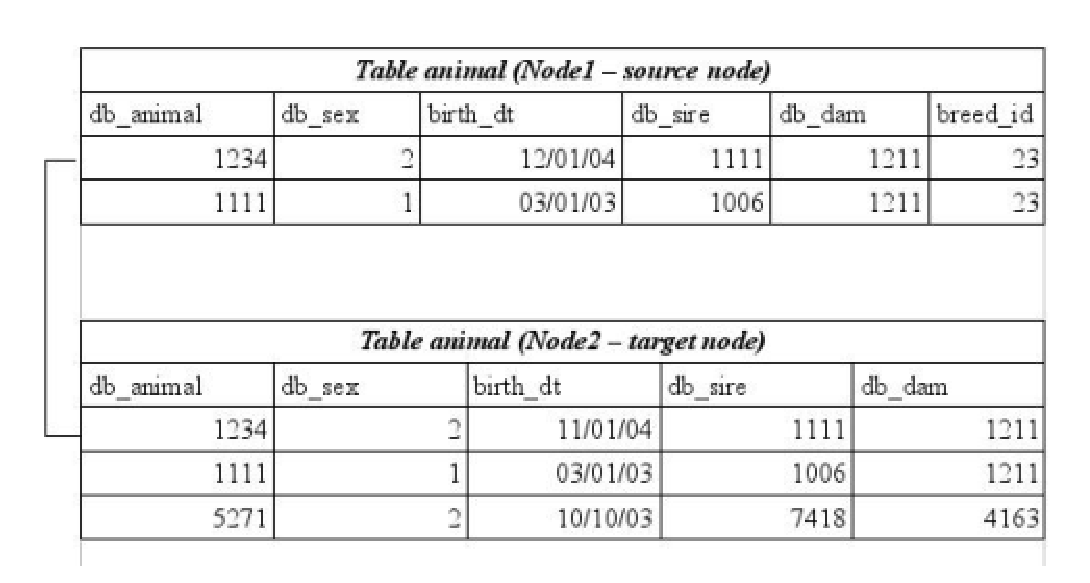
\includegraphics[%
  width=1.0\linewidth]{./synchronization/tables.eps}\end{center}

\begin{center}Information part: (1234,2,12/01/04,1111,1211)\end{center}
\end{figure}
\\
Two nodes can exchange information by setting source/target fields
of the desired data element. For consistency reasons the following
rule should apply: The source field of DE in the receiver node is
the address of the sender node and the target field of the sender
contains the receiver address . \\
This data flow, managed by setting source/target fields is regulated
by Network manager in cooperation with all nodes, thus preventing
inconsistencies in the system.\\
Also, as stated before, only owner can make representative changes
of a data element and this changes are obligatory for all other nodes.

In a generic system there will be three type of nodes:

\begin{itemize}
\item nodes that are only sources of information for the others
\item nodes that are only targets
\item nodes that are sources for some data elements and targets for other
data elements
\end{itemize}
An example of such general animal biodiversity system topology is
shown on Figure \ref{cap:General-system-topology}.%
\begin{figure}

\caption{General system topology\label{cap:General-system-topology}}

\begin{center}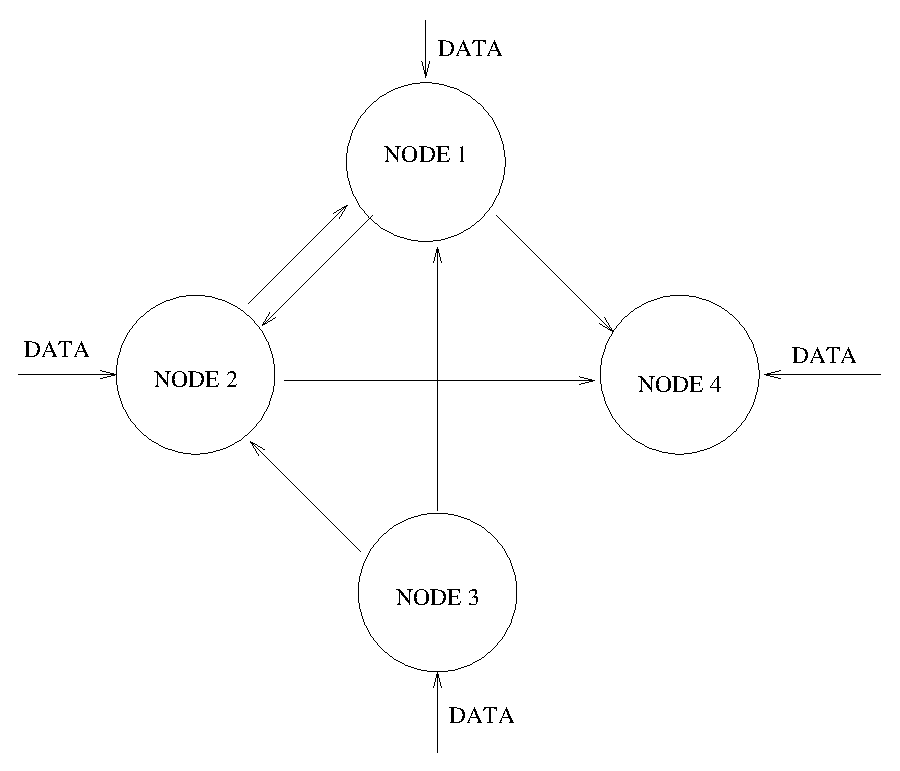
\includegraphics[%
  width=1.0\linewidth,
  keepaspectratio]{./synchronization/univtopology.eps}\end{center}
\end{figure}
 NODE3 is an example of the first kind, NODE4 - of the second and
NODE1 and NODE2 are examples of the third kind. In this example the
content of NODE4 will look like on Figure \ref{cap:NODE4-data-content}.
%
\begin{figure}

\caption{NODE4 data content\label{cap:NODE4-data-content}}

\begin{center}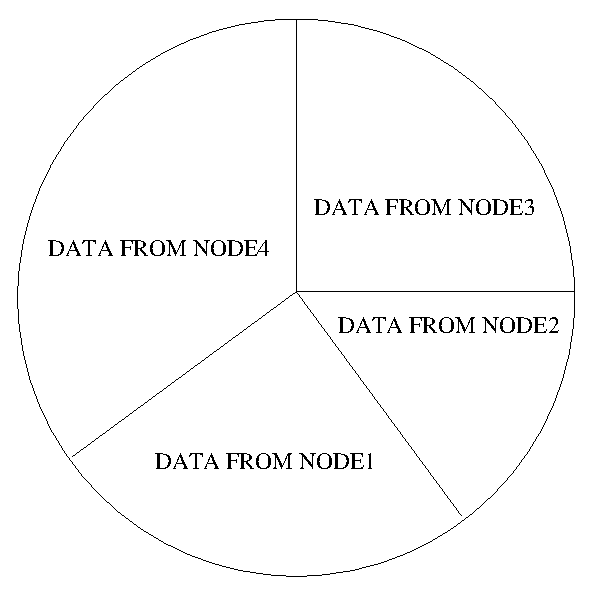
\includegraphics{./synchronization/nodedata.eps}\end{center}
\end{figure}
In the defined above terms {}``Data from NODE3'' means data owned
by NODE3 (initially loaded in NODE3). This data can be received via
NODE1 or NODE2 and the route depends on the source-target pairs. It
is possible that part of the data elements are distributed via NODE1
and part - via NODE2, but it is not possible that one data element
has NODE1 and NODE2 as sources simultaneously.


\section{Functional model}

The functional model of the synchronization process of farm animal
data is shown on Figure \ref{cap:Functional-model}. %
\begin{figure}

\caption{Functional model\label{cap:Functional-model}}

\begin{center}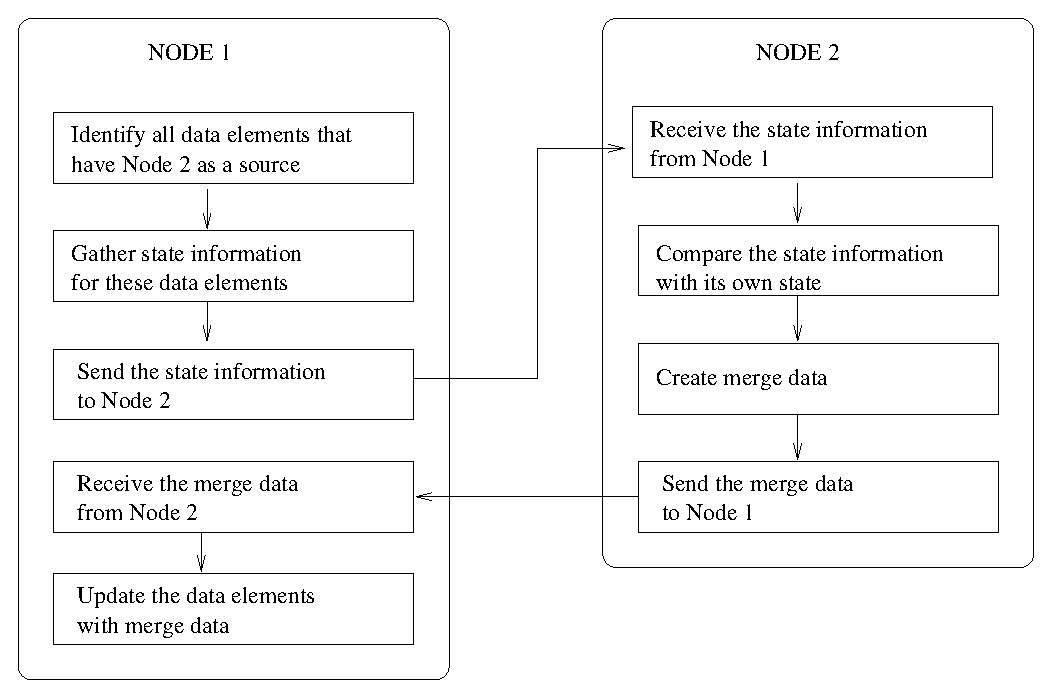
\includegraphics[%
  width=1.0\linewidth]{./synchronization/functmodel.eps}\end{center}
\end{figure}

\section{Implementation}
The implementation has to include the following steps:
\begin{itemize}
\item Setting unique node name\\
Each node has to have unique name within the APIIS-network. THis name is given by the local administrator, but has to be co-ordinated with the Network Manager. The name is set in the local '/etc/apiisrc' file.

\begin{verbatim}
[SYNCHRONISATION]
node_name = EAAP
\end{verbatim} 

\item Setting unique node ip\_address
Each node must have static ip\_address which is accessible from each node within the network. In addition port 5431 has to be open for incomming connections (this is the port where the server daemon listens). The ip\_address is also set in local '/etc/apiisrc' file

\begin{verbatim}
[SYNCHRONISATION]
node_ip = 10.1.1.126
\end{verbatim} 

\item Setting unique numbering interval
Each node in the system has to have unique record numbers and also unique animal internal numbers. The numbering range has to be obtained from from Network Manager and set in local '/etc/apiisrc' file:

\begin{verbatim}
[SYNCHRONISATION]
sequence_interval=1:100000000
\end{verbatim} 

The initialization of all sequence generators is done via the 'CreateDatabase' subroutine. It encapsulates the subroutines: 'LoadNodeData' and 'SetSequences' which are responsible for loading the local nodename and address in the database and setting the numbering interval for all sequences.
\item Setting information about the other nodes in the network
This is done via the program 'nodemanagement.pl' using the menu Settings$>$Nodes.
\item Setting information about the sources
This is done via the program 'nodemanagement.pl' using the menu Settings$>$Sources.
\item Setting information about the targets
This is done via the program 'nodemanagement.pl' using the menu Settings$>$Targets.
\end{itemize}


\chapter{Internationalization in APIIS}
This chapter deals with the localization (internationalization?) aspects
and the design in APIIS. Here, we distinguish two parts:
\begin{itemize}
\item localization of interfaces
\item localization of database content
\end{itemize} 
\section{Localization of Interfaces}
Helmut: hier kennst Du Dich aus.
\section{Multilanguage Handling of Database Content}
In the EFABIS database we have much database content that needs to be available in a number of languages. These are for instance breed descriptions, codes like male and female. With national database feeding their data into the regional database at the EAAP breed descriptions will have to be in the national language, while for the upper levels (EAAP and FAO) these will have to be in one of the official languages. As a result, if data are to be entered for a public record at the national level a national and an international version of the same field will have to be supplied.
Operationally, only the international version will go the regional level, while the national information will stay where it is. Being public data, the new record will go up the FAO. From there it will go down to a translator, all via the standard synchronization protocol. The translator will create a new record in a new official language, this will then via the same protocol go down to the regional and finally national level.
Thus, there will be private (local) and public (international) data for one entity.
\subsection{Implementation}
\subsubsection{Database Structure}
Starting point is a table that initially contains multilingual content, i.e. text columns that will appear in more than one language. The procedure followed is:
\begin{enumerate}
\item split the table into a part that contains only columns which do not need translation, i.e. numerical values. This part will keep the original primary key. For the breeds table in EFABIS this will be the breed\_id.
\item have another part that contains all those columns that need translation, one row per language. Accordingly, the primary key will be composed from the original primary key (the breed\_id in the EFABIS example) and the language. This will be a pointer to langugages table where we have ISO language code eg. PL or EN and other language description.
\end{enumerate} 
An example is given in table \ref{master}. This is the "master" with PK breed\_id while the second table \ref{translation} has a unique key consisting of breed\_id and language.


\begin{table}
\caption{master part}\label {master}
\begin{center}\begin{tabular}{|c|c|c|}
\hline breed\_id (PK) &male  &female  \\ 
\hline 25 & 2 & 0 \\ 
\hline 26 & 0 & 2 \\ 
\hline 
\end{tabular} \end{center}
\end{table}


\begin{table}
\caption {translation part}
\label{translation}\begin{center}\begin{tabular}{|c|c|c|}
\hline  breed\_id& language\_id &shape  \\ 
\hline  25&  2&  Dlugie krecone rogi\\ 
\hline  25&  1&  Long curved horn\\ 
\hline 
\end{tabular} \end{center}
\end{table}

Some tables will not be splited into two parts eg. CODES. Primary key of is defined as conactenated from ext\_code, class and lang\_id where closing date is NULL. Aditional table for language information was added (see table \ref{langtable}).


\begin{table}
\caption {language table}
\label{langtable}\begin{center}\begin{tabular}{|c|c|c|}
\hline  lang\_id& iso\_lang& lang  \\ 
\hline  1&  EN&  English\\ 
\hline  2&  PL&  Polski or Polish?\\ 
\hline 
\end{tabular} \end{center}
\end{table}

Generaly tables which have translatable primary key or part of primary key
will not be splited into two tables. Columns ext\_name in naming table and
ext\_unit in unit table are not translatable. 

\subsubsection{Encoding}
Currently, encoding relies on one language only. Extension to a multi language setting will be made through views. Views will mask tables used for current coding/encoding only for one language. Thus views will be created dinamicly in user schema. Name of view will be same as table name.
\normalsize
Language views will be created after access right views. 
Thus, in a load object we want to insert the translation of a German and English text. Assuming that the column 'shape' is encoded in the model file, then the pseudo SQL in a load object will look like:
\scriptsize {\begin{verbatim}
        set_lang=>'DE';$lang='DE';
        $pseudo_sql[1] =
         'INSERT INTO breeds_lang_horns (
                      lang,
		      breed_id,
                      shape
                 ) VALUES (
		      $lang,
                      $breed_id,
                      'gerade'
                 )';
        set_lang=>'EN'; $lang='EN';
        $pseudo_sql[1] =
         'INSERT INTO breeds_lang_horns (
	              lang,
                      breed_id,
                      shape
                 ) VALUES (
		      $lang,
                      $breed_id,
                      'straight'
                 )';
		 
\end{verbatim} }
\normalsize
The call to the object set\_lang (Apiis->language?) will set the language for the encoding to either 'DE' or 'EN' and create or recreate aproporiate views for codding/encoding.

\subsection{Meta level}

The meta layer will be treated as before.
(Zhivko???: The meta level should be based on the view system build for one language.)
Probably it will be the only change there.

\begin{itemize}
\item Inserting a new record\\
\scriptsize{
SELECT \$breed\_id FROM breeds WHERE mcname=\$mcname AND country\_id=\$country\_id
AND tax\_id=\$tax\_id;\\
INSERT INTO breeds\_horns\_master (breed\_id,male,female) VALUES (\$breed\_id,\$male,\$female);\\
INSERT INTO breeds\_horns\_transl (breed\_id,lang\_id,shape) VALUES
(\$breed\_id,\$lang,\$shape\_pl);\\
INSERT INTO breeds\_horns\_transl (breed\_id,lang\_id,shape) VALUES
(\$breed\_id,\$lang1,\$shape\_en);
\item Updating existing record\\
SELECT \$breed\_id FROM breeds WHERE mcname=\$mcname AND country\_id=\$country\_id
AND tax\_id=\$tax\_id;\\
UPDATE breeds\_horns\_master SET male=\$male WHERE breed\_id=\$breed\_id;\\
UPDATE breeds\_horns\_transl SET shape=\$shape\_en WHERE breed\_id=\$breed\_id
AND lang\_id=\$lang1;
}
\end{itemize}
\normalsize
All statements have be wrapped in one transaction block.


\subsection{Access rights}

Again the Access rights system should be revisited, but probably will
stay the same. There should be only mechanism for consistency of the
user rights, i.e. if he can enter the most common name (which is in
the master table because is not translatable), he has to be able to
enter the language of the most common name (which is in the translation
table).


\subsection{Synchronization}

Since the structure will be the same on all levels and we have clear
mechanism to mark the records to be synchronized the synchronization
will remain the same. All records to be synchronized will be marked
manually by the user.
\subsection{Outputs}
Outputs could be routed via views which can bre created (automatically?)
   for each language. It would simply present the master and translation
   table as one for a given language via a join on the primary key of the
   master with the primary key and languange (which should be a unique
         composite index) for the translation table.
\section{International Character Sets}
Localized languages require for their presentation a corresponding character set. 
Therefore, we do not only need to take note of the correct character set that goes with a language but also need to be able to use them appropriately. It is the problem to work with many different character encodings. Two character encodings can use the same number representation for two different characters, or use different numbers for the same character. Any given computer (especially servers) needs to support many different encodings. Now whenever data are sending between different encodings or platforms there is a risk of data coruption when we don't use aproporiate character encoding. The best way is use one character encoding which can cover all languages used in a system. The best way here is to use UNICODE standards.

\subsection{UNICODE}

Unicode and ISO/IEC 10646 are coordinated standards that provide code points for characters in almost all modern character set standards, covering more than 30 writing systems and hundreds of languages, including important modern languages. All characters in the largest Chinese, Japanese, and Korean dictionaries are also encoded. Unicode 1.0 was released in October 1991, and 4.0 in April 2003.
A Unicode character is an abstract entity. Unicode provides a unique number for every character, no matter what the platform, no matter what the program, no matter what the language.

\subsection{Support for UNICODE}

UNICODE is supported in many operating systems, all modern browsers, database and programming enviroments. PostgreSQL database hass support of UNICODE (from version 7.1). After using UNICODE as a database character encoding we can sotre any language in database text field, if we want we can generate outputs in other encodings eg. LATIN2 because Postgres has support for automatic characters encoding but is better to use one character encoding everywhere.
 Perl is also supporting Unicode characters (from version 5.6, but more complete support is in Perl form version 5.8). Perl should automaticly work with strings encoded in Unicode correctly. If we want also use variables name encoded in Unicode  we need to specify this with Perl pragma:\\
\scriptsize{
use encoding 'utf8';
}
\normalsize
after that we can use variables name with national characters. Perl characters representations is hidden from user. Perl scripts should work whit unicode date same as with data encodet for eg. latin but it depends on operating system enviroment. Probabyl we need examine regular expressions for unicode compatibility because we now will have much wider characters set then in eg. LATIN encoding. In some places we need accept not only [A-Za-z] characters but also some national special characters as German �, �, �  etc.  with  [:alpha:] (see perlre documentation for more).
For user interface it should be no problem to use unicode for web interface, also a Tk interface is working with unicode (form version 8.00) only need correct font to show all characters.


\subsection{Locales and fonts}

For proper working of Unicode settings in database or in Perl script we also need to use LOCALE settings. Locale are important when we are sorting and comparing strings with national characters. By default Perl is ignoring locale settings if we want to use it we need to specify it:\\
\scriptsize{
use locale;
}
\normalsize
This is needed if we for eg. want to change character case with lc or uc function in Perl. If we don't specify this that Perl will not change case correctly for all characters in our string. Most of Perl operators don't need to know about characters in string. If there are utf8 characters in is working with utf8 characters. Generaly is hiding internal representation of characters from outside world.
\\
Unicode is platform endependent but if we want to use national characters on some operating system we need to have approperite fonts which can show all characters described in Unicode. It is mostly important for languages like Chinese, Japanese, Korean, Arabic etc.

\begin{itemize}
\item how do we handle latin based character sets?
\item what about others like cyrilic?
\item even more complicated: what about Arabic, Chinese, Japaneze etc?
\item do we have to go UNICODE?
\item what can be put in a filed of type text in the database? Using a local keyboard and the appropriate character set, can we store Bulgarian in one row and French or Chineze in others?
\end{itemize}

\section{The Core}
\subsection{Apiis.pm\label{Apiis_pm}\index{Apiis.pm}}




\subsubsection*{SYNOPSIS\label{Apiis_pm_SYNOPSIS}\index{Apiis pm!SYNOPSIS}}
\begin{verbatim}
   use Apiis;
   Apiis->initialize( VERSION => '$Revision: 1.4 $' );
\end{verbatim}
\subsubsection*{DESCRIPTION\label{Apiis_pm_DESCRIPTION}\index{Apiis pm!DESCRIPTION}}


\textbf{initialize} is the primary method for executables to load the Apiis
system. It does basic checking, creates, and exports the \$apiis object into
the main namespace.



To avoid numerous nasty error messages you are strongly advised to start
your program with this BEGIN block:

\begin{verbatim}
   BEGIN {
      use Env qw( APIIS_HOME );
      die "\n\tAPIIS_HOME is not set!\n\n" unless $APIIS_HOME;
      push @INC, "$APIIS_HOME/lib";
   }
\end{verbatim}


This catches errors due to an unset APIIS\_HOME environment variable and
adds \$APIIS\_HOME/lib to your library path to find the Apiis modules.

\subsubsection*{SUBROUTINES\label{Apiis_pm_SUBROUTINES}\index{Apiis pm!SUBROUTINES}}
\paragraph*{initialize\label{Apiis_pm_initialize}\index{Apiis pm!initialize}}


\textbf{initialize} loads Apiis::Init, creates a new Apiis::Init object and
assigns it to the global variable \$apiis, which is exported by default.
Also exported is the global subroutine \_\_() for nationalisation of the
code.



\textbf{initialize} currently takes one (hash) argument:

\begin{verbatim}
   Apiis->initialize( VERSION => '$Revision: 1.4 $' );
\end{verbatim}


It propagetes the cvs version as the program version and can be retrieved
with \$apiis-$>$version.

\subsubsection*{Author\label{Apiis_pm_Author}\index{Apiis pm!Author}}


Helmut Lichtenberg $<$heli@tzv.fal.de$>$

\subsection{Apiis::Init -- Basic initialisation object for the complete APIIS structure\label{Apiis::Init_--_Basic_initialisation_object_for_the_complete_APIIS_structure}\index{Apiis::Init -- Basic initialisation object for the complete APIIS structure}}




\subsubsection*{SYNOPSIS\label{Apiis::Init_--_Basic_initialisation_object_for_the_complete_APIIS_structure_SYNOPSIS}\index{Apiis::Init -- Basic initialisation object for the complete APIIS structure!SYNOPSIS}}
\begin{verbatim}
   our $apiis = Apiis::Init->new(
     version     => $version,
         programname => $programname
   );
\end{verbatim}


This is the basic module for spreading the APIIS configuration during
runtime.  It is invoked automatically if you run the common
initialisation block which includes \$APIIS\_HOME/lib/apiis\_init.pm. You
can access this basic object via the global variable \$apiis.

\subsubsection*{DESCRIPTION\label{Apiis::Init_--_Basic_initialisation_object_for_the_complete_APIIS_structure_DESCRIPTION}\index{Apiis::Init -- Basic initialisation object for the complete APIIS structure!DESCRIPTION}}


Apiis::Init creates an internal structure and public methods to access
this structure.



Public and internal methods are:

\subsubsection*{INTERNAL METHODS\label{Apiis::Init_--_Basic_initialisation_object_for_the_complete_APIIS_structure_INTERNAL_METHODS}\index{Apiis::Init -- Basic initialisation object for the complete APIIS structure!INTERNAL METHODS}}
\paragraph*{new (mostly internal)\label{Apiis::Init_--_Basic_initialisation_object_for_the_complete_APIIS_structure_new_mostly_internal_}\index{Apiis::Init -- Basic initialisation object for the complete APIIS structure!new (mostly internal)}}


new creates the object where we usually refer to as \$apiis.

\paragraph*{\_init (internal)\label{Apiis::Init_--_Basic_initialisation_object_for_the_complete_APIIS_structure__init_internal_}\index{Apiis::Init -- Basic initialisation object for the complete APIIS structure!\ init (internal)}}


\_init does the main initialization and creates the internal structure for:



APIIS\_HOME os\_user version programname date\_format
entry\_views reserved\_strings language codes\_table browser fileselector



This is done by querying parameter from the operating system (username) and
the user environment (APIIS\_HOME). APIIS\_LOCAL is set after a certain
project is selected and the model file is joined into \$apiis.



The main resources for this basic structure are the configuration files
\$APIIS\_HOME/etc/apiisrc and later \$APIIS\_LOCAL/etc/apiisrc.

\paragraph*{\_get\_user\_from\_os (internal)\label{Apiis::Init_--_Basic_initialisation_object_for_the_complete_APIIS_structure__get_user_from_os_internal_}\index{Apiis::Init -- Basic initialisation object for the complete APIIS structure!\ get\ user\ from\ os (internal)}}


The username \$apiis-$>$os\_user is determined by the operating system. This is
mainly needed for initial log messages, who started the program.

\paragraph*{projects (public)\label{Apiis::Init_--_Basic_initialisation_object_for_the_complete_APIIS_structure_projects_public_}\index{Apiis::Init -- Basic initialisation object for the complete APIIS structure!projects (public)}}


Returns the names of the projects defined in \$APIIS\_HOME/etc/apiisrc.

\paragraph*{project (public)\label{Apiis::Init_--_Basic_initialisation_object_for_the_complete_APIIS_structure_project_public_}\index{Apiis::Init -- Basic initialisation object for the complete APIIS structure!project (public)}}


Returns the \$APIIS\_LOCAL path for a specific project and is therefore mostly
redundant with \$apiis-$>$APIIS\_LOCAL().



Example:

\begin{verbatim}
   $local_path = $apiis->project('ref_breedprg');
\end{verbatim}
\paragraph*{formpath (public)\label{Apiis::Init_--_Basic_initialisation_object_for_the_complete_APIIS_structure_formpath_public_}\index{Apiis::Init -- Basic initialisation object for the complete APIIS structure!formpath (public)}}


Returns the default path for a specific project where the form definitions are
stored, usually at \$APIIS\_LOCAL/etc/forms. This default location is set during
join\_model.



It can be set to a different value with:



Example:

\begin{verbatim}
   $apiis->formpath( './forms' );
\end{verbatim}
\paragraph*{l10n\_init (public)\label{Apiis::Init_--_Basic_initialisation_object_for_the_complete_APIIS_structure_l10n_init_public_}\index{Apiis::Init -- Basic initialisation object for the complete APIIS structure!l10n\ init (public)}}


\textbf{l10n\_init} does the localisation from Apiis::I18N::L10N. The language is
passed as input parameter.



The failure handler for Locale::Maketext is set to return the untranslated
english string (default language).



Also the defined projects translations table is imported into the l10n
schema.



Input: language



Output: none

\paragraph*{l10n\_import (public)\label{Apiis::Init_--_Basic_initialisation_object_for_the_complete_APIIS_structure_l10n_import_public_}\index{Apiis::Init -- Basic initialisation object for the complete APIIS structure!l10n\ import (public)}}


\textbf{l10n\_import} imports an additional lexicon. This is usually done by
\textbf{l10n\_init}. In case you want to load another lexicon, use \textbf{l10n\_import}.



Input:

\begin{verbatim}
   1. language
   2. file
\end{verbatim}


Output: none



Example:

\begin{verbatim}
   $self->l10n_import( $lang, $lexicon ) if -f $lexicon;
\end{verbatim}
\paragraph*{\_\_()\label{Apiis::Init_--_Basic_initialisation_object_for_the_complete_APIIS_structure__}\index{Apiis::Init -- Basic initialisation object for the complete APIIS structure!\ \ ()}}


After initialization of the language handle \$lh:

\begin{verbatim}
   $lh = Apiis::L10N->get_handle( $apiis->language );
\end{verbatim}


you could write for localising text:

\begin{verbatim}
   print $lh->maketext('Just another Perl hacker'), "\n";
\end{verbatim}


To make it more convenient I created a shortcut wrapper around this,
the subroutine \_\_(). So you can write:

\begin{verbatim}
   print __('Just another Perl hacker'), "\n";
\end{verbatim}


Note: I must use an anonymous subroutine to have access to \$lh. See
'Programming Perl', p. 976 for error message: 'Variable "\$lh" will not stay
shared'.



Note2: The bare underscore \_ is treated specially, as it is always forced into
the package main ( like \$\_, @\_ ). See "Programming Perl', p. 591.
So we don't have to export it.



Note3: The single underscore \_ produced errors several times when it clashed
with the "Perl special filehandle used to cache the information from the
last successfull stat, lstat, or file test operator". ('Programming Perl',
p. 657).
This global underline subroutine is used e.g. in the CPAN or CGI modules. So
it's better to *not* use \_() for localisation. Preferred shortcut now is
\_\_().  (5. Aug. 2004 - heli)

\paragraph*{\_add\_obj (internal)\label{Apiis::Init_--_Basic_initialisation_object_for_the_complete_APIIS_structure__add_obj_internal_}\index{Apiis::Init -- Basic initialisation object for the complete APIIS structure!\ add\ obj (internal)}}


\$self-$>$\_add\_obj is used to mount an additional object structure into the
apiis core structure. An example is the addition of the model file
information under \$apiis-$>$Model.



usage:

\begin{verbatim}
   $self->_add_obj(
      Model  => [ $mod_obj ],
      caller => [ $package, $file, $line ]
   );
\end{verbatim}
\subsubsection*{PUBLIC METHODS\label{Apiis::Init_--_Basic_initialisation_object_for_the_complete_APIIS_structure_PUBLIC_METHODS}\index{Apiis::Init -- Basic initialisation object for the complete APIIS structure!PUBLIC METHODS}}
\paragraph*{\$apiis-$>$[ os\_user $|$ APIIS\_HOME $|$ version $|$ programname $|$ date\_format $|$ entry\_views $|$ reserved\_strings $|$ codes\_table $|$ browser $|$ fileselector $|$ use\_filelog $|$ filelog\_filename $|$use\_syslog $|$ syslog\_facility $|$ use\_sql\_logging $|$ sql\_logfile $|$ sql\_log\_dml\_only $|$ node\_name $|$ node\_ip $|$ sequence\_interval $|$ multilanguage ] (all public)\label{Apiis::Init_--_Basic_initialisation_object_for_the_complete_APIIS_structure__apiis-_os_user_APIIS_HOME_version_programname_date_format_entry_views_reserved_strings_codes_table_browser_fileselector_use_filelog_filelog_filename_use_syslog_syslog_facility_use_sql_logging_sql_logfile_sql_log_dml_only_node_name_node_ip_sequence_interval_multilanguage_all_public_}\index{Apiis::Init -- Basic initialisation object for the complete APIIS structure!\$apiis-$>$[ os\ user $|$ APIIS\ HOME $|$ version $|$ programname $|$ date\ format $|$ entry\ views $|$ reserved\ strings $|$ codes\ table $|$ browser $|$ fileselector $|$ use\ filelog $|$ filelog\ filename $|$use\ syslog $|$ syslog\ facility $|$ use\ sql\ logging $|$ sql\ logfile $|$ sql\ log\ dml\ only $|$ node\ name $|$ node\ ip $|$ sequence\ interval $|$ multilanguage ] (all public)}}


These public methods provide an interface for the user to access the
internal structure.



They are readonly and usually return a scalar value except entry\_views and
reserved\_strings.



\$apiis-$>$entry\_views returns a hash reference with the table names as keys
and the according entry views (which only contain active records of this
table) as values:

\begin{verbatim}
   codes => entry_codes
   unit => entry_unit
   transfer => entry_transfer
\end{verbatim}


\$apiis-$>$reserved\_strings returns a hash reference to the names and values
of the reserved strings for data entry:

\begin{verbatim}
   v_concat => ' >=< '
\end{verbatim}


(One problem here could be the intended blanks as part of the delimiter.
 Maybe they get lost by reading the config file with Config::IniFiles.)

\paragraph*{\$apiis-$>$[ language ] (public)\label{Apiis::Init_--_Basic_initialisation_object_for_the_complete_APIIS_structure__apiis-_language_public_}\index{Apiis::Init -- Basic initialisation object for the complete APIIS structure!\$apiis-$>$[ language ] (public)}}


\textbf{language} is a public read/write method. Initially it's populated by the
apiisrc configuration files, but it can be changed during program
execution. When you set a new language, the old one is returned:

\begin{verbatim}
   my $oldlang = $apiis->language( <newlang> );
\end{verbatim}
\paragraph*{\$apiis-$>$[ date\_order $|$ time\_order $|$ extdate2iso $|$ iso2extdate $|$ exttime2iso $|$ iso2exttime $|$ date\_parts $|$ time\_parts $|$ isodate $|$ isotime $|$ date\_sep $|$ time\_sep $|$ date\_conf\_err $|$ time\_conf\_err ] (public)\label{Apiis::Init_--_Basic_initialisation_object_for_the_complete_APIIS_structure__apiis-_date_order_time_order_extdate2iso_iso2extdate_exttime2iso_iso2exttime_date_parts_time_parts_isodate_isotime_date_sep_time_sep_date_conf_err_time_conf_err_public_}\index{Apiis::Init -- Basic initialisation object for the complete APIIS structure!\$apiis-$>$[ date\ order $|$ time\ order $|$ extdate2iso $|$ iso2extdate $|$ exttime2iso $|$ iso2exttime $|$ date\ parts $|$ time\ parts $|$ isodate $|$ isotime $|$ date\ sep $|$ time\ sep $|$ date\ conf\ err $|$ time\ conf\ err ] (public)}}


The Apiis default format for date and time accords to the widely accepted
ISO 8601 standard. Have a look at

\begin{verbatim}
   http://www.cl.cam.ac.uk/~mgk25/iso-time.html
\end{verbatim}


for a good summary or other resources for detailed descriptions. You are
strongly encouraged, to also use ISO 8601 date formats in your software.



\textbf{date\_order} returns the initially in apiisrc defined order of the date as
a scalar string. You can set the date format during program execution (e.g.
when you batch process several data streams) in the following syntax:

\begin{verbatim}
   my $oldformat = $apiis->date_order(
      order => 'DD.MM.YYYY',
      sep   => '.',
   );
\end{verbatim}


The two required parameters are the order of the parts and the separator.
The string to define the order has the following limitations:

\begin{itemize}

\item only the separator and the capital letters Y, M, and D are allowed.
\item the year has to be specified in the 4 digit form YYYY to avoid
     ambiguity.
\item the day (DD) and month (MM) formats have 2 digits each.
\item a valid order string with separators therefore must have the length of
     10 characters.
\item a valid order string without separator must have the length of 8
     characters.
\item for year, month, and day values only digits are allowed.\end{itemize}


Example without separator:

\begin{verbatim}
   my $oldformat = $apiis->date_order(
      order => 'YYYYMMDD',
      sep   => '',
   );
\end{verbatim}


If you want to set \textbf{date\_order} to new values, it returns a reference to
the hash of the previously configured parameters order and sep. You thus
can reset the old date format with:

\begin{verbatim}
   $apiis->date_order( %$oldformat );
\end{verbatim}


If the chosen date order accords to ISO 8601 (YYYY-MM-DD) the status flag
\$apiis-$>$isodate() is set to 1, otherwise its 0. The same applies to the
time order (hh:mm:ss) and isotime().



Another flag \textbf{date\_conf\_err()} is internally used to mark a bad date
format configuration and as a result of it skip all date tests.



If you really have to parse dates on your own you can get the separators
(besides the format string with \textbf{date\_order}) by invoking:

\begin{verbatim}
   my $d_sep = $apiis->date_sep();
   my $t_sep = $apiis->time_sep();
\end{verbatim}


\textbf{date\_parts()} is a readonly public methods that returns an array (or an
arrayref, depending on the invoking context) of the configured parts of the
date format in the correct order (e.g. ["YYYY", "MM", "DD"]).



This method is mainly usefull in internal date calculations.



\textbf{extdate2iso} converts your external date format into the internal
ISO 8601 format.  It additionally checks, if the passed date is valid.



In scalar context, a formatted date string is returned. In list context,
you get the date parts in the shown order:

\begin{verbatim}
   Example:
   $apiis->date_order( order => 'DD.MM.YYYY', sep => '.' );
\end{verbatim}
\begin{verbatim}
   # scalar context;
   my $ext_date = '11.2.2005 13:37:00';
   print $apiis->extdate2iso($ext_date), "\n";
   # prints: 2005-02-11 13:37:00
\end{verbatim}
\begin{verbatim}
   # list context:
   my ( $year, $month, $day, $hour, $minute, $second )
      = $apiis->extdate2iso($ext_date);
\end{verbatim}


The same return schema for scalar and list context applies to
\textbf{exttime2iso}, \textbf{iso2extdate}, and \textbf{iso2exttime}.



Note, that also the \textbf{iso2extdate} and \textbf{iso2exttime} methods keep this order in
list context. It does not make sense to make them return in the configured
external order as the list context is useful for programming purposes and a
changing order would force you to parse the configuration. And this is not,
what you want.

\paragraph*{substitute\_env (internal)\label{Apiis::Init_--_Basic_initialisation_object_for_the_complete_APIIS_structure_substitute_env_internal_}\index{Apiis::Init -- Basic initialisation object for the complete APIIS structure!substitute\ env (internal)}}


Does some postprocessing for special cases (substitution of APIIS\_HOME and
APIIS\_LOCAL with their values).



The value to check for substituting is passed as a reference so that
substituting is done in place:

\begin{verbatim}
   $self->substitute_env( \$val_to_substitute );
\end{verbatim}


It doesn't matter if there is a dollar sign \$ in front of APIIS\_HOME and
APIIS\_LOCAL or not.

\paragraph*{\_join\_user (internal)\label{Apiis::Init_--_Basic_initialisation_object_for_the_complete_APIIS_structure__join_user_internal_}\index{Apiis::Init -- Basic initialisation object for the complete APIIS structure!\ join\ user (internal)}}


\textbf{\$apiis-}\_join\_user$>$ takes a hashref with a User object (required) and
verifies this user against the database. If it's a valid user, his data gets
mounted into the \$apiis structure as the User object.



Example:
   \$apiis-$>$\_join\_user( \{ userobj =$>$ \$user\_obj \} );

\paragraph*{exists\_user (public)\label{Apiis::Init_--_Basic_initialisation_object_for_the_complete_APIIS_structure_exists_user_public_}\index{Apiis::Init -- Basic initialisation object for the complete APIIS structure!exists\ user (public)}}


\$apiis-$>$exists\_user returns 1 if the User object is already mounted into the
\$apiis structure, 0 otherwise.

\paragraph*{use\_filelog/use\_syslog/use\_sql\_logging (public)\label{Apiis::Init_--_Basic_initialisation_object_for_the_complete_APIIS_structure_use_filelog_use_syslog_use_sql_logging_public_}\index{Apiis::Init -- Basic initialisation object for the complete APIIS structure!use\ filelog/use\ syslog/use\ sql\ logging (public)}}


These methods mainly reflect the settings in apiisrc. They are read/write to
enable changing these values in rare cases, e.g. when running check\_integrity,
where logging make only little sense.

\paragraph*{syslog\_priority/filelog\_priority (public)\label{Apiis::Init_--_Basic_initialisation_object_for_the_complete_APIIS_structure_syslog_priority_filelog_priority_public_}\index{Apiis::Init -- Basic initialisation object for the complete APIIS structure!syslog\ priority/filelog\ priority (public)}}


syslog\_priority is read/write although it mostly won't be overwritten. But
in some cases you may want to switch the logging level for a certain part
of the code to e.g. 'debug', while other parts stay at e.g. 'warn'.
The allowed priorities are debug, info, notice, warn, warning, error, err, crit,
alert, emerg, panic in this order (err = error, warn = warning, emerg =
panic).



If syslog\_priority is set with

\begin{verbatim}
   my $oldvalue = $apiis->syslog_priority('debug');
\end{verbatim}


it returns the old value of syslog\_priority. You then can reset it with

\begin{verbatim}
   $apiis->syslog_priority( $oldvalue );
\end{verbatim}


Otherwise it returns the current value of syslog\_priority.



The same applies to \textbf{filelog\_priority}.

\paragraph*{log\_priority (public)\label{Apiis::Init_--_Basic_initialisation_object_for_the_complete_APIIS_structure_log_priority_public_}\index{Apiis::Init -- Basic initialisation object for the complete APIIS structure!log\ priority (public)}}


\textbf{log\_priority} is write-only and sets the values of syslog\_priority and
filelog\_priority to the same value which is passed as the argument. This is
mainly a development help as you don't know if the configuration is just set
to syslog or filelog.

\paragraph*{debug (public)\label{Apiis::Init_--_Basic_initialisation_object_for_the_complete_APIIS_structure_debug_public_}\index{Apiis::Init -- Basic initialisation object for the complete APIIS structure!debug (public)}}


\textbf{debug} returns 1 if the debug level is set, 0 otherwise.
Any true input value sets \$self-$>$debug to 1, any false value to 0.



\textbf{debug} can be used to query or set a debug flag, which can be used to
prevent the expensive invokation of \$apiis-$>$log on debug level. This flag
depends on the settings of filelog\_priority and syslog\_priority. If either of
them is set to 'debug', \$self-$>$debug always returns 1, even if you pass 0
to it. If you set \$self-$>$debug(1), filelog\_priority and syslog\_priority keep
their values;

\paragraph*{log (public)\label{Apiis::Init_--_Basic_initialisation_object_for_the_complete_APIIS_structure_log_public_}\index{Apiis::Init -- Basic initialisation object for the complete APIIS structure!log (public)}}
\begin{verbatim}
   $apiis->log('warn', "Cannot open file: $!");
\end{verbatim}


or

\begin{verbatim}
   $apiis->log('warn', 'Cannot open file: %s', $!);
\end{verbatim}


log() is the interface to the syslog utility. It takes as first input
parameter the syslog priority, at which it shall be printed into the system
log files (debug info notice warn warning error err crit alert emerg
panic). All levels below \$apiis-$>$syslog\_priority are suppressed, all of
\$apiis-$>$syslog\_priority and above are sent to syslog.



As an addition it can also log the sql statements into a file for basic
database recovery. It the passed priority is of type 'sql' like in

\begin{verbatim}
   $apiis->log('sql', $sqltext);
\end{verbatim}


and use\_sql\_logging is set to a true value in apiisrc, the sqltext will get
logged into the configured sql\_logfile together with a timestamp,
dabasename, and username (in a separate line with a sql comment). After a
defined backup state you simply have to run this file through your favorite
frontend to the database to recover the current state. If sql\_log\_dml\_only
is true in apiisrc, select statements are not logged.
Messages of priority 'sql' are not passed to syslog.

\paragraph*{status (public)\label{Apiis::Init_--_Basic_initialisation_object_for_the_complete_APIIS_structure_status_public_}\index{Apiis::Init -- Basic initialisation object for the complete APIIS structure!status (public)}}


\$apiis-$>$status returns a general status which is accessible everywhere and
at any time during execution. A status of 0 means success, all true values
indicate an error.



If you pass a parameter this will set the status to this value.

\paragraph*{running\_check\_integrity (public)\label{Apiis::Init_--_Basic_initialisation_object_for_the_complete_APIIS_structure_running_check_integrity_public_}\index{Apiis::Init -- Basic initialisation object for the complete APIIS structure!running\ check\ integrity (public)}}


\$apiis-$>$running\_check\_integrity is a simple switch that has to be set in
the program check\_integrity. Some checks on record level have different
behaviour (less checks) if they are invoked by check\_integrity.

\paragraph*{check\_status (public)\label{Apiis::Init_--_Basic_initialisation_object_for_the_complete_APIIS_structure_check_status_public_}\index{Apiis::Init -- Basic initialisation object for the complete APIIS structure!check\ status (public)}}


Checks \$apiis-$>$status and prints errors (if any). Optionally dies above a
certain severity level and ignores errors below a certain security level.



Input parameter can be a hash with the keys:

\begin{itemize}

\item \textbf{die} -- you can pass a level of severity to let the program die
        at this point and all levels above (in severity).
\item \textbf{ignore} -- below this level of severity the error messages are ignored\end{itemize}


\textbf{check\_status} returns the boolean value of the status stored in
\$obj-$>$status().



Example:

\begin{verbatim}
   $apiis->check_status(
       die => 'CRIT',
       ignore => 'INFO',
   );
\end{verbatim}
\paragraph*{errors (public)\label{Apiis::Init_--_Basic_initialisation_object_for_the_complete_APIIS_structure_errors_public_}\index{Apiis::Init -- Basic initialisation object for the complete APIIS structure!errors (public)}}


\$apiis-$>$errors returns the stored errors as an array of objects or an array
reference, just as requested by the caller.
If new errors are stored, errors() returns the error id(s). If you store
one error object, the error id of this error is returned as a scalar. If
you store an array of error objects, an array or arrayref of the error ids
of these error objects is returned in the order of the error objects.



Examples:
   my \$err\_id      = \$apiis-$>$errors(\$error\_object);
   my @err\_ids     = \$apiis-$>$errors(@error\_objects);
   my \$err\_ids\_ref = \$apiis-$>$errors(@error\_objects);

\paragraph*{error (public)\label{Apiis::Init_--_Basic_initialisation_object_for_the_complete_APIIS_structure_error_public_}\index{Apiis::Init -- Basic initialisation object for the complete APIIS structure!error (public)}}


\$apiis-$>$error takes as parameter an error id and returns the error object
for this id. This enables you to write code like this:

\begin{verbatim}
   $apiis->error(3)->print;
   $apiis->error(4)->severity('CRIT');
\end{verbatim}


If you pass an invalid error id, an error object is created and passed back
to the caller.

\paragraph*{del\_errors (public)\label{Apiis::Init_--_Basic_initialisation_object_for_the_complete_APIIS_structure_del_errors_public_}\index{Apiis::Init -- Basic initialisation object for the complete APIIS structure!del\ errors (public)}}


\$apiis-$>$del\_errors deletes all error objects.

\paragraph*{del\_error (public)\label{Apiis::Init_--_Basic_initialisation_object_for_the_complete_APIIS_structure_del_error_public_}\index{Apiis::Init -- Basic initialisation object for the complete APIIS structure!del\ error (public)}}


\$apiis-$>$del\_error takes as parameter an error id and deletes this error object
from the \$apiis-$>$errors array. Example:

\begin{verbatim}
   $apiis->del_error(3);
\end{verbatim}


If you pass an invalid error id, an error object is created, added to
\$apiis-$>$errors and additionally passed back to the caller.

\paragraph*{localtime (public)\label{Apiis::Init_--_Basic_initialisation_object_for_the_complete_APIIS_structure_localtime_public_}\index{Apiis::Init -- Basic initialisation object for the complete APIIS structure!localtime (public)}}


\$apiis-$>$localtime provides you with an unformatted timestamp. Usually this
is not used. The preferred methods are \$apiis-$>$today and \$apiis-$>$now as
they convert the date/time to the localized format.



\$apiis-$>$localtime returns a list of parameters. Example:

\begin{verbatim}
   my ($year, $mon, $mday, $hour, $min, $sec)
      = $apiis->localtime;
\end{verbatim}
\paragraph*{today (public)\label{Apiis::Init_--_Basic_initialisation_object_for_the_complete_APIIS_structure_today_public_}\index{Apiis::Init -- Basic initialisation object for the complete APIIS structure!today (public)}}


\$apiis-$>$today returns a formatted string of the current day.

\paragraph*{now (public)\label{Apiis::Init_--_Basic_initialisation_object_for_the_complete_APIIS_structure_now_public_}\index{Apiis::Init -- Basic initialisation object for the complete APIIS structure!now (public)}}


\$apiis-$>$now returns a formatted string of the current day and time.
For internal use it accepts an input parameter

\begin{verbatim}
   $apiis->now( format => 'today' );
\end{verbatim}


to return only the day without time. This is the whole magic behind
\$apiis-$>$today. :\^{})

\paragraph*{join\_model (public)\label{Apiis::Init_--_Basic_initialisation_object_for_the_complete_APIIS_structure_join_model_public_}\index{Apiis::Init -- Basic initialisation object for the complete APIIS structure!join\ model (public)}}


\textbf{\$apiis-}join\_model("modelfile")$>$ mounts all informations of the model file
into the core apiis structure and provides methods to access them.



As required input you have to provide the key 'userobj'. The value must be a
valid User-object.



Example:

\begin{verbatim}
   $apiis->join_model('breedprg',
      userobj => $user_obj,
   );
\end{verbatim}


\textbf{join\_model} creates an Apiis::Model object and passes it to \_add\_obj.
With the key 'Model', the model object is passed as the first and
only element of an anon array reference.



Besides the model file name there is another (hash) parameter 'database' to
\textbf{join\_model}.



With 'database =$>$ 0', the model file will be joined into \$apiis without
connection to the database.  For later joining the database into \$apiis, use
the public method \textbf{\$apiis-}join\_database$>$.



Using \textbf{join\_model} without connecting to the database will be
used in quite rare cases. One usefull operation will be when you want to
drop the complete database during basic initialisation.
In this case you have to provide some dummy User object like:

\begin{verbatim}
   require Apiis::DataBase::User;
   my $dummy = Apiis::DataBase::User->new(
       id       => ($apiis->os_user || 'nobody'),
       password => 'nopassword',
   );
\end{verbatim}
\begin{verbatim}
   $apiis->join_model('breedprg',
      userobj => $dummy,
      database => 0,
   );
\end{verbatim}
\paragraph*{exists\_model (public)\label{Apiis::Init_--_Basic_initialisation_object_for_the_complete_APIIS_structure_exists_model_public_}\index{Apiis::Init -- Basic initialisation object for the complete APIIS structure!exists\ model (public)}}


\$apiis-$>$exists\_model returns 1 if the model file is already mounted into the
\$apiis structure, 0 otherwise.

\paragraph*{\_join\_database (internal)\label{Apiis::Init_--_Basic_initialisation_object_for_the_complete_APIIS_structure__join_database_internal_}\index{Apiis::Init -- Basic initialisation object for the complete APIIS structure!\ join\ database (internal)}}


\$apiis-$>$\_join\_database initializes the database access.



It adds the newly created Apiis::DataBase::Init object into the existing
\$apiis-tree with the key 'DataBase':

\paragraph*{join\_database (public)\label{Apiis::Init_--_Basic_initialisation_object_for_the_complete_APIIS_structure_join_database_public_}\index{Apiis::Init -- Basic initialisation object for the complete APIIS structure!join\ database (public)}}


\$apiis-$>$join\_database is simply a public wrapper for \_join\_database.



The public method join\_database is usually not needed as join\_model()
automatically joins the database into \$apiis. For some rare cases (e.g.
initial creation of database), you can join\_model() without connection to
the database by passing the parameter 'database =$>$ 0'.



So
   \$apiis-$>$join\_model('breedprg', database =$>$ 0);
   \$apiis-$>$join\_database;



is equivalent to
   \$apiis-$>$join\_model('breedprg');

\paragraph*{exists\_database (public)\label{Apiis::Init_--_Basic_initialisation_object_for_the_complete_APIIS_structure_exists_database_public_}\index{Apiis::Init -- Basic initialisation object for the complete APIIS structure!exists\ database (public)}}


\$apiis-$>$exists\_database returns 1 if the database initialisation is already
done, 0 otherwise. The existance of the database object does not
necessarily include the database connection. If you invoke join\_model with
the parameter 'database =$>$ 0' the database object is created without
connecting to the database. This is needed for special cases like mksql,
where you need the configuration data like the db-specific datatype for the
metatypes like TIMESTAMP to create the database.

\paragraph*{exists\_auth (public)\label{Apiis::Init_--_Basic_initialisation_object_for_the_complete_APIIS_structure_exists_auth_public_}\index{Apiis::Init -- Basic initialisation object for the complete APIIS structure!exists\ auth (public)}}


\textbf{exists\_auth} is a boolean switch to show, if the Auth object for
authentication/authorisation is joined into the global \$apiis structure. It is
0/undef, if no Auth object/method exists, 1 otherwise.

\paragraph*{get\_db\_conf (mainly internal)\label{Apiis::Init_--_Basic_initialisation_object_for_the_complete_APIIS_structure_get_db_conf_mainly_internal_}\index{Apiis::Init -- Basic initialisation object for the complete APIIS structure!get\ db\ conf (mainly internal)}}


Read the config file for the passed Database from
\$APIIS\_HOME/etc/apiis/$<$Database$>$.conf and return a hash reference of this
structure.

\paragraph*{AUTOLOAD (internal)\label{Apiis::Init_--_Basic_initialisation_object_for_the_complete_APIIS_structure_AUTOLOAD_internal_}\index{Apiis::Init -- Basic initialisation object for the complete APIIS structure!AUTOLOAD (internal)}}


\textbf{AUTOLOAD()} catches all invocations of methods, that don't exist. On this
level it makes mainly sense for the structural elements Cache, Model,
DataBase, User, etc. It's difficult to catch them otherwise in
expressions like \$apiis-$>$Model-$>$tables, when join\_model has failed before
and therefore no method Model() exists. This case usually produces Error
objects, but every developer is free to ignore them.



Currently some more or less useful error messages are generated, printed
to STDOUT and the process dies. This is not optimal for processes that run
in a grapical environment (Tk, Html) and don't have access to a terminal.
But does it make sense to create an Error object if the developer tends to
ignore them?



Additionally, the produced error message is stored in the logfile/syslog,
if configured.

\subsection{Apiis::Init::Config mainly ready apiisrc config files\label{Apiis::Init::Config_mainly_ready_apiisrc_config_files}\index{Apiis::Init::Config mainly ready apiisrc config files}}




\subsubsection*{DESCRIPTION\label{Apiis::Init::Config_mainly_ready_apiisrc_config_files_DESCRIPTION}\index{Apiis::Init::Config mainly ready apiisrc config files!DESCRIPTION}}


Apiis::Init::Config contains internal methods to read the different apiisrc
files.

\subsubsection*{METHODS\label{Apiis::Init::Config_mainly_ready_apiisrc_config_files_METHODS}\index{Apiis::Init::Config mainly ready apiisrc config files!METHODS}}
\paragraph*{\_import\_apiisrc (internal)\label{Apiis::Init::Config_mainly_ready_apiisrc_config_files__import_apiisrc_internal_}\index{Apiis::Init::Config mainly ready apiisrc config files!\ import\ apiisrc (internal)}}


Imports the default apiis config file \$APIIS\_HOME/etc/apiisrc.

\paragraph*{\_import\_apiisrc\_local (internal)\label{Apiis::Init::Config_mainly_ready_apiisrc_config_files__import_apiisrc_local_internal_}\index{Apiis::Init::Config mainly ready apiisrc config files!\ import\ apiisrc\ local (internal)}}


Overwrites the defaults from apiis apiisrc config file with the
project specific one.

\paragraph*{\_import\_user\_apiisrc (internal)\label{Apiis::Init::Config_mainly_ready_apiisrc_config_files__import_user_apiisrc_internal_}\index{Apiis::Init::Config mainly ready apiisrc config files!\ import\ user\ apiisrc (internal)}}


Overwrites the project definition from global apiisrc config file.
This can be used for developers on a multiuser server to point to their
private copy of the project tree.



It reads only the [PROJECTS] section of apiisrc.

\paragraph*{\_xml2model (internal)\label{Apiis::Init::Config_mainly_ready_apiisrc_config_files__xml2model_internal_}\index{Apiis::Init::Config mainly ready apiisrc config files!\ xml2model (internal)}}


\textbf{\_xml2model} parses the passed xmlfile and returns a reference to a
datastructure, representing the model file.



usage:

\begin{verbatim}
    eval { $href = $self->Apiis::Init::Config::_xml2model(
                       xmlfile => $filename
                   );
    };
\end{verbatim}


This results in a structure like this:

\begin{verbatim}
    $href->{
       general => {...},
       table   => {
          <tablename> => {
             struct_type => '...',
             trigger  => {...},
             sequence => [...],
             index    => [...],
             pk       => {...},
             column   => {
                <columnname> => {...},
                <columnname> => {...},
             },
             _column_order => [...],
          },
       },
       _table_order => [...],
    };
\end{verbatim}


Only for internal use.



Note: This method will disappear in the near future when the model file
structure and parsing is rewritten.

\paragraph*{\_get\_db\_conf (internal)\label{Apiis::Init::Config_mainly_ready_apiisrc_config_files__get_db_conf_internal_}\index{Apiis::Init::Config mainly ready apiisrc config files!\ get\ db\ conf (internal)}}


Read the config file for the passed Database from
\$APIIS\_HOME/etc/apiis/$<$Database$>$.conf and return a hash reference of this
structure.

\subsubsection*{\$apiis-$>$\_check\_date\_conf (internal)\label{_apiis-_check_date_conf_internal_}\index{\$apiis-$>$\ check\ date\ conf (internal)}}


Internal routine to run some checks on the configured date format.
Sets the \_date\_parts array in case of success.

\subsubsection*{\$apiis-$>$\_check\_time\_conf (internal)\label{_apiis-_check_time_conf_internal_}\index{\$apiis-$>$\ check\ time\ conf (internal)}}


Internal routine to run some checks on the configured time format.
Sets the \_time\_parts array in case of success.

\subsection{SYNOPSIS\label{SYNOPSIS}\index{SYNOPSIS}}
\begin{verbatim}
   $xml_obj = Apiis::Init::XML->new(%args);
   $xml_obj = Apiis::Init::XML->new(
         dtd=>$dtd_file,
         xml=>$xml_file,
         gui=>$what_type_of_gui
   );
\end{verbatim}
\subsection{DESCRIPTION\label{DESCRIPTION}\index{DESCRIPTION}}


XML.pm init a file of configuration written in xml. XML.pm merge definitions
from the configuration file and the default values from the dtd-scheme.



Suppositions:



Each xml-element need a unique name over all configuration and subconfiguration
files, which will be defined in "Name". Access to each attribute take place with
a method in combination with the name of the element:

\begin{verbatim}
   xml:
    <PageHeader Name="PageHeader_10">
      <Lines Name="Line_1" Column="1-4" Row="1" LineType="solid"/>
    </PageHeader>             
    ---------
\end{verbatim}
\begin{verbatim}
   code: 
    $c=$xml_obj->Line_1->LineType
    $c is "solid"
\end{verbatim}
\begin{verbatim}
    $c=$xml_obj->Line_1->Name
    $c is "Line_1"
\end{verbatim}


Independent of the xml-definition a complete set of methods will be initiate
depend on the definition in the dtd-scheme. The default settings come from the
dtd-scheme and will overwritten if a the same attribute is defined in the
xml-scheme. E.g.

\begin{verbatim}
   dtd: 
   <!ATTLIST Text  
           Name       ID                          #REQUIRED
           Content    CDATA                       #REQUIRED
           Position   (static|absolute|relative)  "relative"
   >
\end{verbatim}
\begin{verbatim}
  xml:
  <PageHeader Name="PageHeader_10">
     <Text Position="relative" Name="Text_1" Content="test"/>
  </PageHeader>
\end{verbatim}
\begin{verbatim}
  code: 
   $c=$xml_obj->Text_1->Position
   $c is "relative"
\end{verbatim}


Each xml-file has a hierachical structure. XML makes a flat structure.

\subsection{METHODS\label{METHODS}\index{METHODS}}
\subsubsection*{\$apiis-$>$GUI-$>$[fullname $|$ basename $|$ ext $|$ path $|$ gui\_file ] (all public, readonly)\label{_apiis-_GUI-_fullname_basename_ext_path_gui_file_all_public_readonly_}\index{\$apiis-$>$GUI-$>$[fullname $|$ basename $|$ ext $|$ path $|$ gui\ file ] (all public, readonly)}}


fullname, basename, ext, path provide the fullname (basename.extension),
basename (without extension), extension, and path of the gui file.

\subsection{Apiis::Model -- methods to access the model file data via the \$apiis
structure\label{Apiis::Model_--_methods_to_access_the_model_file_data_via_the_apiis_structure}\index{Apiis::Model -- methods to access the model file data via the \$apiis
structure}}




\subsubsection*{SYNOPSIS\label{Apiis::Model_--_methods_to_access_the_model_file_data_via_the_apiis_structure_SYNOPSIS}\index{Apiis::Model -- methods to access the model file data via the apiis structure!SYNOPSIS}}
\begin{verbatim}
   $apiis->join_model('breedprg');
\end{verbatim}


The configuration data of the model file is mounted into the \$apiis
structure simply by running the join\_model method with the model file name
as the only parameter.

\subsubsection*{DESCRIPTION\label{Apiis::Model_--_methods_to_access_the_model_file_data_via_the_apiis_structure_DESCRIPTION}\index{Apiis::Model -- methods to access the model file data via the apiis structure!DESCRIPTION}}


This Model.pm module provides an object and the appropriate access methods.
With join\_model they are passed to Apiis::Init.pm and there with \_add\_obj
added to the global structure

\subsubsection*{METHODS\label{Apiis::Model_--_methods_to_access_the_model_file_data_via_the_apiis_structure_METHODS}\index{Apiis::Model -- methods to access the model file data via the apiis structure!METHODS}}
\paragraph*{new (mostly internal)\label{Apiis::Model_--_methods_to_access_the_model_file_data_via_the_apiis_structure_new_mostly_internal_}\index{Apiis::Model -- methods to access the model file data via the apiis structure!new (mostly internal)}}


Apiis::Model-$>$new is mainly invoked by Apiis::Init. The user interface is
join\_model.

\paragraph*{\_init (internal)\label{Apiis::Model_--_methods_to_access_the_model_file_data_via_the_apiis_structure__init_internal_}\index{Apiis::Model -- methods to access the model file data via the apiis structure!\ init (internal)}}


\_init does the main initialization and creates the internal structure to
keep the model file values.

\paragraph*{\$apiis-$>$Model-$>$[fullname $|$ basename $|$ ext $|$ path $|$ db\_driver $|$ db\_name
$|$ db\_host $|$ db\_port $|$ db\_user $|$ db\_password $|$ max\_check\_level] (all public, readonly)\label{Apiis::Model_--_methods_to_access_the_model_file_data_via_the_apiis_structure__apiis-_Model-_fullname_basename_ext_path_db_driver_db_name_db_host_db_port_db_user_db_password_max_check_level_all_public_readonly_}\index{Apiis::Model -- methods to access the model file data via the apiis structure!\$apiis-$>$Model-$>$[fullname $|$ basename $|$ ext $|$ path $|$ db\ driver $|$ db\ name
$|$ db\ host $|$ db\ port $|$ db\ user $|$ db\ password $|$ max\ check\ level] (all public, readonly)}}


fullname, basename, ext, path provide the fullname (basename.extension),
basename (without extension), extension, and path of the model file.



The db\_... methods reflect the database configurations at the top of the
model file.



max\_check\_level gives you the maximal configured checklevel of this model
file, if anybody really needs it.

\paragraph*{tables (public, readonly)\label{Apiis::Model_--_methods_to_access_the_model_file_data_via_the_apiis_structure_tables_public_readonly_}\index{Apiis::Model -- methods to access the model file data via the apiis structure!tables (public, readonly)}}


\$apiis-Model-$>$tables returns the names of the defined tables. If you want
an array, it gives you an array of these tables. If you want a scalar, you
also get what you want, a reference to the same array.

\paragraph*{table (public, readonly)\label{Apiis::Model_--_methods_to_access_the_model_file_data_via_the_apiis_structure_table_public_readonly_}\index{Apiis::Model -- methods to access the model file data via the apiis structure!table (public, readonly)}}
\begin{verbatim}
   $apiis->Model->table( $tablename );
\end{verbatim}


returns an object of Apiis::Model::TableObj for this tablename.

\paragraph*{check\_level (public, read/write)\label{Apiis::Model_--_methods_to_access_the_model_file_data_via_the_apiis_structure_check_level_public_read_write_}\index{Apiis::Model -- methods to access the model file data via the apiis structure!check\ level (public, read/write)}}
\begin{verbatim}
   my $current_level = $apiis->Model->check_level;
   my $old_level = $apiis->Model->check_level(2);
      ... do some work
   $apiis->Model->check_level( $old_level );
\end{verbatim}


Without an parameter check\_level returns the current check level. You can
change the current check level by passing the new level to check\_level,
which then returns the old check level.



check\_level also tests, if a passed new level is numeric and does not
exceed the maximum defined level in the model file.

\subsubsection*{Apiis::Model::TableObj -- internal package to provide a table object with
methods to access a single table and its columns\label{Apiis::Model_--_methods_to_access_the_model_file_data_via_the_apiis_structure_Apiis::Model::TableObj_--_internal_package_to_provide_a_table_object_with_methods_to_access_a_single_table_and_its_columns}\index{Apiis::Model -- methods to access the model file data via the apiis structure!Apiis::Model::TableObj -- internal package to provide a table object with
methods to access a single table and its columns}}




\paragraph*{SYNOPSIS\label{Apiis::Model::TableObj_--_internal_package_to_provide_a_table_object_with_methods_to_access_a_single_table_and_its_columns_SYNOPSIS}\index{Apiis::Model::TableObj -- internal package to provide a table object with methods to access a single table and its columns!SYNOPSIS}}


Programming interface:

\begin{verbatim}
   $table_obj = Apiis::Model::TableObj->new( $tablename, $struct_ref);
\end{verbatim}


Usage:

\begin{verbatim}
   $table_obj = $apiis->Model->table('animal');
\end{verbatim}
\paragraph*{METHODS\label{Apiis::Model::TableObj_--_internal_package_to_provide_a_table_object_with_methods_to_access_a_single_table_and_its_columns_METHODS}\index{Apiis::Model::TableObj -- internal package to provide a table object with methods to access a single table and its columns!METHODS}}
\subparagraph*{new (mostly internal)\label{Apiis::Model::TableObj_--_internal_package_to_provide_a_table_object_with_methods_to_access_a_single_table_and_its_columns_new_mostly_internal_}\index{Apiis::Model::TableObj -- internal package to provide a table object with methods to access a single table and its columns!new (mostly internal)}}


To create the table object, new() needs as input the table name and a
reference to the datastructure of this table from the model file:

\begin{verbatim}
   $table_obj = Apiis::Model::TableObj->new( $tablename, $struct_ref);
\end{verbatim}


The order of the columns in the model file is preserved.

\subparagraph*{column (public, readonly)\label{Apiis::Model::TableObj_--_internal_package_to_provide_a_table_object_with_methods_to_access_a_single_table_and_its_columns_column_public_readonly_}\index{Apiis::Model::TableObj -- internal package to provide a table object with methods to access a single table and its columns!column (public, readonly)}}


\$table\_obj-$>$column( \$col\_name ) returns the column object for this column

\subparagraph*{name (public, readonly)\label{Apiis::Model::TableObj_--_internal_package_to_provide_a_table_object_with_methods_to_access_a_single_table_and_its_columns_name_public_readonly_}\index{Apiis::Model::TableObj -- internal package to provide a table object with methods to access a single table and its columns!name (public, readonly)}}


\$table\_obj-$>$name returns the name of this table.

\subparagraph*{struct\_type (public, readonly)\label{Apiis::Model::TableObj_--_internal_package_to_provide_a_table_object_with_methods_to_access_a_single_table_and_its_columns_struct_type_public_readonly_}\index{Apiis::Model::TableObj -- internal package to provide a table object with methods to access a single table and its columns!struct\ type (public, readonly)}}


\$table\_obj-$>$struct\_type returns the structural type of this table.
Current values of struct\_type can be mandatory, recommended, and optional.

\subparagraph*{columns/cols (public, readonly)\label{Apiis::Model::TableObj_--_internal_package_to_provide_a_table_object_with_methods_to_access_a_single_table_and_its_columns_columns_cols_public_readonly_}\index{Apiis::Model::TableObj -- internal package to provide a table object with methods to access a single table and its columns!columns/cols (public, readonly)}}


\$table\_obj-$>$cols returns the columns of this table.
\$table\_obj-$>$columns is just an alias.

\subparagraph*{primarykey (public, readonly)\label{Apiis::Model::TableObj_--_internal_package_to_provide_a_table_object_with_methods_to_access_a_single_table_and_its_columns_primarykey_public_readonly_}\index{Apiis::Model::TableObj -- internal package to provide a table object with methods to access a single table and its columns!primarykey (public, readonly)}}


primarykey() needs one argument, which is either 'ref\_col', 'view',
'where', or 'concat'.

\begin{verbatim}
   $table_obj->primarykey('ref_col')
\end{verbatim}


returns the reference column to which this primary key in the table refers
to.

\begin{verbatim}
   $table_obj->primarykey('concat')
\end{verbatim}


returns the external columns, that build the concatenated primary key. The
old syntax of \$table\_obj-$>$primarykey('ext\_cols') is still supported but
deprecated.

\begin{verbatim}
   $table_obj->primarykey('view')
\end{verbatim}


returns the viewname of the view, that finally provides the foreignkey
through the where clause:

\begin{verbatim}
   $table_obj->primarykey('where')
\end{verbatim}


Often the where clause is 'closing\_dt is NULL'. The resulting view then
shows only records, which are not closed.

\subparagraph*{\$table\_obj-$>$[sequence $|$ sequences $|$ index $|$ indices $|$ indexes] (public,
readonly)\label{Apiis::Model::TableObj_--_internal_package_to_provide_a_table_object_with_methods_to_access_a_single_table_and_its_columns__table_obj-_sequence_sequences_index_indices_indexes_public_readonly_}\index{Apiis::Model::TableObj -- internal package to provide a table object with methods to access a single table and its columns!\$table\ obj-$>$[sequence $|$ sequences $|$ index $|$ indices $|$ indexes] (public,
readonly)}}


They return the index and the sequence entries for the table,
either as an array or as an array reference. There are only two
methods, the others act like aliases.



usage:

\begin{verbatim}
   my @indices = $table_obj->indices;
   my $sequences_ref = $table_obj->sequences;
\end{verbatim}
\subparagraph*{\$table\_obj-$>$triggers( \$triggertype ) (public, readonly)\label{Apiis::Model::TableObj_--_internal_package_to_provide_a_table_object_with_methods_to_access_a_single_table_and_its_columns__table_obj-_triggers_triggertype_public_readonly_}\index{Apiis::Model::TableObj -- internal package to provide a table object with methods to access a single table and its columns!\$table\ obj-$>$triggers( \$triggertype ) (public, readonly)}}


The method \textbf{triggers} takes the following triggertypes as argument:

\begin{verbatim}
   $table_obj->triggers( 'preinsert' );
   $table_obj->triggers( 'postinsert' );
   $table_obj->triggers( 'preupdate' );
   $table_obj->triggers( 'postupdate' );
   $table_obj->triggers( 'predelete' );
   $table_obj->triggers( 'postdelete' );
\end{verbatim}


and returns the triggers for this type. Depending on the calling context
they will be returned as a list or as an array reference.

\subparagraph*{\$table\_obj-$>$[datatype $|$ length $|$ default $|$ description $|$ check $|$ modify $|$ foreignkey $|$ label] (public, readonly)\label{Apiis::Model::TableObj_--_internal_package_to_provide_a_table_object_with_methods_to_access_a_single_table_and_its_columns__table_obj-_datatype_length_default_description_check_modify_foreignkey_label_public_readonly_}\index{Apiis::Model::TableObj -- internal package to provide a table object with methods to access a single table and its columns!\$table\ obj-$>$[datatype $|$ length $|$ default $|$ description $|$ check $|$ modify $|$ foreignkey $|$ label] (public, readonly)}}


Although these methods are column methods, they are kept here for
compatibility reasons.



The old, still valid (but deprecated) syntax

\begin{verbatim}
   my $descr = $table_obj->description( $column_name );
\end{verbatim}


should now be better written as:

\begin{verbatim}
   my $descr = $column_obj->description;
\end{verbatim}


or

\begin{verbatim}
   my $descr = $table_obj->column( $column_name )->description;
\end{verbatim}
\paragraph*{Apiis::Model::ColumnObj -- internal package to provide a column object with
methods to access a single column of a table\label{Apiis::Model::TableObj_--_internal_package_to_provide_a_table_object_with_methods_to_access_a_single_table_and_its_columns_Apiis::Model::ColumnObj_--_internal_package_to_provide_a_column_object_with_methods_to_access_a_single_column_of_a_table}\index{Apiis::Model::TableObj -- internal package to provide a table object with methods to access a single table and its columns!Apiis::Model::ColumnObj -- internal package to provide a column object with
methods to access a single column of a table}}




\subparagraph*{SYNOPSIS\label{Apiis::Model::ColumnObj_--_internal_package_to_provide_a_column_object_with_methods_to_access_a_single_column_of_a_table_SYNOPSIS}\index{Apiis::Model::ColumnObj -- internal package to provide a column object with methods to access a single column of a table!SYNOPSIS}}
\begin{verbatim}
   $col_obj = $table_obj->column( $column_name );
\end{verbatim}
\subparagraph*{DESCRIPTION\label{Apiis::Model::ColumnObj_--_internal_package_to_provide_a_column_object_with_methods_to_access_a_single_column_of_a_table_DESCRIPTION}\index{Apiis::Model::ColumnObj -- internal package to provide a column object with methods to access a single column of a table!DESCRIPTION}}
\subparagraph*{METHODS\label{Apiis::Model::ColumnObj_--_internal_package_to_provide_a_column_object_with_methods_to_access_a_single_column_of_a_table_METHODS}\index{Apiis::Model::ColumnObj -- internal package to provide a column object with methods to access a single column of a table!METHODS}}
\*{\$column\_obj-$>$[datatype $|$ length $|$ default $|$ description $|$ check $|$ modify $|$ struct\_type $|$ label] (public, readonly)\label{Apiis::Model::ColumnObj_--_internal_package_to_provide_a_column_object_with_methods_to_access_a_single_column_of_a_table__column_obj-_datatype_length_default_description_check_modify_struct_type_label_public_readonly_}\index{Apiis::Model::ColumnObj -- internal package to provide a column object with methods to access a single column of a table!\$column\ obj-$>$[datatype $|$ length $|$ default $|$ description $|$ check $|$ modify $|$ struct\ type $|$ label] (public, readonly)}}


Example:
   my \$datatype = \$column\_obj-$>$datatype;



The according values from the model file are returned. All these
methods are readonly.



check() returns the rules for the current check level. If a check level
for a column is defined/exists, this one is taken.



If there is no CHECKn defined for check level n the default CHECK is taken.
This also applies if e.g. CHECK2 is defined in the model file but no
CHECK1. In this case the default CHECK is taken for CHECK1 as this is
undef.

\*{foreignkey (public, readonly)\label{Apiis::Model::ColumnObj_--_internal_package_to_provide_a_column_object_with_methods_to_access_a_single_column_of_a_table_foreignkey_public_readonly_}\index{Apiis::Model::ColumnObj -- internal package to provide a column object with methods to access a single column of a table!foreignkey (public, readonly)}}
\begin{verbatim}
   my ($fk_table, $fk_column) = $column_obj->foreignkey;
\end{verbatim}


foreignkey() returns the defined foreign key table and the foreign key
column for this column, either as an array or as a
reference to an array, depending on the callers context.



It returns undef if no foreign key is defined.

\subsection{Apiis::Errors -- Provide error objects for generic error handling in APIIS\label{Apiis::Errors_--_Provide_error_objects_for_generic_error_handling_in_APIIS}\index{Apiis::Errors -- Provide error objects for generic error handling in APIIS}}




\subsubsection*{SYNOPSIS\label{Apiis::Errors_--_Provide_error_objects_for_generic_error_handling_in_APIIS_SYNOPSIS}\index{Apiis::Errors -- Provide error objects for generic error handling in APIIS!SYNOPSIS}}
\begin{verbatim}
   my $err_obj = Apiis::Errors->new(
      type      => 'CONFIG',
      severity  => 'INFO',
      from      => 'test.Errors',
      msg_short => "No date format defined",
   );
\end{verbatim}


Apiis::Errors-$>$new() creates an error object, that describes an error
comprehensively to enable further adequate processing.

\subsubsection*{DESCRIPTION\label{Apiis::Errors_--_Provide_error_objects_for_generic_error_handling_in_APIIS_DESCRIPTION}\index{Apiis::Errors -- Provide error objects for generic error handling in APIIS!DESCRIPTION}}


Apiis::Errors provides an error object with the following traits:

\begin{itemize}

\item Error \textbf{type}, currently:\begin{itemize}

\item \textbf{DATA}    the passed data is not ok (usually in CheckRules)
\item \textbf{DB}      errors from the database (e.g. unique index violation)
\item \textbf{OS}      errors from the operation system (e.g. full hard disk)
\item \textbf{AUTH}    errors concerning access rights
\item \textbf{PARSE}   errors in ParsePseudoSQL with parsing pseudo SQL code
\item \textbf{CODE}    programming errors, e.g. from applications like load objects
\item \textbf{PARAM}   passed parameter is wrong or missing
\item \textbf{CONFIG}  one of the configuration files is wrong or has missing entries
\item \textbf{INSTALL} there is an error in the Apiis/Perl installation
\item \textbf{UNKNOWN} is unknown.\end{itemize}

\item Error \textbf{severity}, currently \textbf{DEBUG INFO NOTICE WARNING ERR CRIT
ALERT EMERG}. These severity values are the same as the unix syslog
priorities. See also 'man syslog.conf' under Unix/Linux.\begin{itemize}

\item \textbf{DEBUG}   debugging messages for bug hunting
\item \textbf{INFO}    informational notice
\item \textbf{NOTICE}  more than information, somebody should notice it
\item \textbf{WARNING} influences further processing but is not so severe
\item \textbf{WARN}    deprecated, use WARNING
\item \textbf{ERR}     error, handled in the normal flow control
\item \textbf{ERROR}   deprecated, use ERR
\item \textbf{CRIT}    critical error, but can be handled under certain circumstances
\item \textbf{ALERT}   alarm, immediate intervention necessary
\item \textbf{EMERG}   no further processing possible (e.g. disk full)
\item \textbf{PANIC}   deprecated, use EMERG\end{itemize}

\item Error \textbf{action}, currently:\begin{itemize}

\item \textbf{INSERT}  the error occurred during a database insert
\item \textbf{UPDATE}  the error occurred during a database update
\item \textbf{DELETE}  the error occurred during a database delete
\item \textbf{SELECT}  the error occurred during a database select
\item \textbf{FETCH}   like SELECT
\item \textbf{DECODE}  the error occurred during an attempt to decode the data
\item \textbf{ENCODE}  the error occurred during an attempt to encode the data
\item \textbf{UNKNOWN} the action is unknown\end{itemize}
\end{itemize}


The internal structure provides the following fields to describe a
certain error:

\begin{verbatim}
 %struct = (
    type           => undef,    # predefined values above
    id             => undef,    # error id
    severity       => undef,    # predefined values above
    action         => undef,    # predefined values above
    from           => undef,    # location where this error comes from
                                # (e.g. sub, rule)
    record_id      => undef,    # id of this record, e.g. record_seq
                                # from inspool
    unit           => undef,    # unit that provides this data
    db_table       => undef,    # database table concerned
    db_column      => undef,    # database column concerned
    data           => undef,    # just handled incorrect data
    ext_fields     => undef,    # involved external fields (array)
    ext_fields_idx => undef,    # index of these external fields (for tabulars)
    ds             => undef,    # data stream name
    err_code       => undef,    # coded error message
    msg_short      => undef,    # main error message for end users
    msg_long       => undef,    # detailed error message
    misc1          => undef,    # user defined scalar
    misc2          => undef,    # user defined scalar
    misc_arr1      => undef,    # user defined array
    misc_arr2      => undef,    # user defined array
    backtrace      => undef,    # backtrace in Carp::longmess style
 );
\end{verbatim}


Public and internal methods are:

\subsubsection*{INTERNAL METHODS\label{Apiis::Errors_--_Provide_error_objects_for_generic_error_handling_in_APIIS_INTERNAL_METHODS}\index{Apiis::Errors -- Provide error objects for generic error handling in APIIS!INTERNAL METHODS}}
\paragraph*{new (mostly internal)\label{Apiis::Errors_--_Provide_error_objects_for_generic_error_handling_in_APIIS_new_mostly_internal_}\index{Apiis::Errors -- Provide error objects for generic error handling in APIIS!new (mostly internal)}}


new creates the object and checks access rights to the object structure.

\paragraph*{\$error\_obj-$>$[ type\_values $|$ severity\_values $|$ action\_values ] (all external)\label{Apiis::Errors_--_Provide_error_objects_for_generic_error_handling_in_APIIS__error_obj-_type_values_severity_values_action_values_all_external_}\index{Apiis::Errors -- Provide error objects for generic error handling in APIIS!\$error\ obj-$>$[ type\ values $|$ severity\ values $|$ action\ values ] (all external)}}


These public methods provide read only access to the preconfigured values.

\paragraph*{\$error\_obj-$>$[ from $|$ line $|$ backtrace $|$ record\_id $|$ unit
            $|$ db\_table $|$ db\_column $|$ data $|$ ext\_fields $|$ ext\_fields\_idx
            $|$ ds $|$ err\_code $|$ msg\_short $|$ msg\_long $|$ misc1 $|$ misc2
            $|$ misc\_arr1 $|$ misc\_arr2 ] (all external)\label{Apiis::Errors_--_Provide_error_objects_for_generic_error_handling_in_APIIS__error_obj-_from_line_backtrace_record_id_unit_db_table_db_column_data_ext_fields_ext_fields_idx_ds_err_code_msg_short_msg_long_misc1_misc2_misc_arr1_misc_arr2_all_external_}\index{Apiis::Errors -- Provide error objects for generic error handling in APIIS!\$error\ obj-$>$[ from $|$ line $|$ backtrace $|$ record\ id $|$ unit
            $|$ db\ table $|$ db\ column $|$ data $|$ ext\ fields $|$ ext\ fields\ idx
            $|$ ds $|$ err\ code $|$ msg\ short $|$ msg\ long $|$ misc1 $|$ misc2
            $|$ misc\ arr1 $|$ misc\ arr2 ] (all external)}}


These public methods provide read/write access to the structur elements.

\paragraph*{print (external)\label{Apiis::Errors_--_Provide_error_objects_for_generic_error_handling_in_APIIS_print_external_}\index{Apiis::Errors -- Provide error objects for generic error handling in APIIS!print (external)}}


Print the defined elements of this error object in the order of the
hash \%struct (actually the @struct array). This is mainly used for debugging.



Second input parameter can be a hash with the key:

\begin{itemize}

\item \textbf{filehandle} -- the output then goes to this filehandle instead of
        STDOUT (default)
        note: the filehandle has to be passed as a typeglob\end{itemize}


Example:

\begin{verbatim}
   $err_obj->print(
      filehandle => *ERR_FILE,
   );
\end{verbatim}
\paragraph*{sprint (external)\label{Apiis::Errors_--_Provide_error_objects_for_generic_error_handling_in_APIIS_sprint_external_}\index{Apiis::Errors -- Provide error objects for generic error handling in APIIS!sprint (external)}}


Return the formatted error message as a string (used by \textbf{print}).

\paragraph*{sprint\_html (external)\label{Apiis::Errors_--_Provide_error_objects_for_generic_error_handling_in_APIIS_sprint_html_external_}\index{Apiis::Errors -- Provide error objects for generic error handling in APIIS!sprint\ html (external)}}


Return the formatted error message as a string (used by \textbf{print}).

\paragraph*{syslog\_print (external)\label{Apiis::Errors_--_Provide_error_objects_for_generic_error_handling_in_APIIS_syslog_print_external_}\index{Apiis::Errors -- Provide error objects for generic error handling in APIIS!syslog\ print (external)}}


The error message is formatted for unix syslog (used by \$apiis-$>$log).

\subsection{Apiis::Misc -- Provides some usefull subroutines, mainly for compatibility reasons\label{Apiis::Misc_--_Provides_some_usefull_subroutines_mainly_for_compatibility_reasons}\index{Apiis::Misc -- Provides some usefull subroutines, mainly for compatibility reasons}}




\subsubsection*{SYNOPSIS\label{Apiis::Misc_--_Provides_some_usefull_subroutines_mainly_for_compatibility_reasons_SYNOPSIS}\index{Apiis::Misc -- Provides some usefull subroutines mainly for compatibility reasons!SYNOPSIS}}
\begin{verbatim}
   use Apiis::Misc qw( <subroutine_name> );
\end{verbatim}
\subsubsection*{DESCRIPTION\label{Apiis::Misc_--_Provides_some_usefull_subroutines_mainly_for_compatibility_reasons_DESCRIPTION}\index{Apiis::Misc -- Provides some usefull subroutines mainly for compatibility reasons!DESCRIPTION}}


Apiis::Misc gives you access to the subroutines (not object methods!):

\begin{verbatim}
   show_progress mychomp elapsed is_true
   Info Error
   LocalToRawDate RawToLocalDate Decode_Date_NativeRDBMS
   find_pod_path file2variable mimetype_of
\end{verbatim}


You can load some of them by writing:

\begin{verbatim}
   use Apiis::Misc qw( show_progress mychomp );
\end{verbatim}


They are also grouped:

\begin{verbatim}
   use Apiis::Misc qw( :Tk );    # exports the Tk routines Info and Error
   use Apiis::Misc qw( :date );  # exports the date routines
   use Apiis::Misc qw( :all );   # exports all routines
\end{verbatim}
\subsubsection*{Subroutines\label{Apiis::Misc_--_Provides_some_usefull_subroutines_mainly_for_compatibility_reasons_Subroutines}\index{Apiis::Misc -- Provides some usefull subroutines mainly for compatibility reasons!Subroutines}}
\paragraph*{show\_progress\label{Apiis::Misc_--_Provides_some_usefull_subroutines_mainly_for_compatibility_reasons_show_progress}\index{Apiis::Misc -- Provides some usefull subroutines mainly for compatibility reasons!show\ progress}}


\textbf{show\_progress} gives you some kind of progress view. It prints a dot every \$mod
times (default 100), every \$mod*10 times it prints the number.
   input:  1.) a reference to the counter (usually starting with 1).
           2.) optional: modulus operator \$mod
   return: none. The counter has to be incremented outside this routine!

\paragraph*{MaskForLatex\label{Apiis::Misc_--_Provides_some_usefull_subroutines_mainly_for_compatibility_reasons_MaskForLatex}\index{Apiis::Misc -- Provides some usefull subroutines mainly for compatibility reasons!MaskForLatex}}


Creates Escape-sequences for print in latex

\paragraph*{mychomp\label{Apiis::Misc_--_Provides_some_usefull_subroutines_mainly_for_compatibility_reasons_mychomp}\index{Apiis::Misc -- Provides some usefull subroutines mainly for compatibility reasons!mychomp}}


By: Chris Nandor (from the Perl Function Repository)
removes end-of-line regardless of originating platform
of file

\paragraph*{Info\label{Apiis::Misc_--_Provides_some_usefull_subroutines_mainly_for_compatibility_reasons_Info}\index{Apiis::Misc -- Provides some usefull subroutines mainly for compatibility reasons!Info}}


show an Tk-Info window

\begin{verbatim}
  usage: Info("Infomessage");
\end{verbatim}
\paragraph*{Error\label{Apiis::Misc_--_Provides_some_usefull_subroutines_mainly_for_compatibility_reasons_Error}\index{Apiis::Misc -- Provides some usefull subroutines mainly for compatibility reasons!Error}}


show an error window

\begin{verbatim}
  usage: Error("Errormessage");
\end{verbatim}
\paragraph*{LocalToRawDate\label{Apiis::Misc_--_Provides_some_usefull_subroutines_mainly_for_compatibility_reasons_LocalToRawDate}\index{Apiis::Misc -- Provides some usefull subroutines mainly for compatibility reasons!LocalToRawDate}}


Date conversion.



Standard SQL format seems to be 'DD-MON-YYYY', e.g. '24-MAY-2000'. At
least PostgreSQL and Oracle6 accept this.
As long as DBI/DBD does not convert different date formats to the standard
formats of the databases we have to provide this conversion in apiis.
Date::Calc has date formats EU (european format day-month-year) and US
(US american format month-day-year)
   input:  type of local dateformat [EU$|$US]
           local date
   return: old version (before Aug. 2001):
           date in native database format or -1 in case of errors
           LocalToRawDate('EU', '24.5.2000') will return '24-MAY-2000'.
           new version:
           list of ( "new\_date\_string", \$status, \$err\_msg )
           LocalToRawDate('EU', '24.5.2000') will return ('24-MAY-2000',0,undef).



Note: This is old stuff and remains here only for compatibility reasons. It
will be removed in the near future. (2005-02-28 heli)

\paragraph*{RawToLocalDate\label{Apiis::Misc_--_Provides_some_usefull_subroutines_mainly_for_compatibility_reasons_RawToLocalDate}\index{Apiis::Misc -- Provides some usefull subroutines mainly for compatibility reasons!RawToLocalDate}}


RawToLocalDate - change native database date format to EU/US-format (Date::Calc)
   input:  type of local dateformat [EU$|$US]
           native database date
   return: date in local format or -1 in case of errors



RawToLocalDate('EU', '24-MAY-2000') will return '24.5.2000'.



Note: This is old stuff and remains here only for compatibility reasons. It
will be removed in the near future. (2005-02-28 heli)

\paragraph*{Decode\_Date\_NativeRDBMS\label{Apiis::Misc_--_Provides_some_usefull_subroutines_mainly_for_compatibility_reasons_Decode_Date_NativeRDBMS}\index{Apiis::Misc -- Provides some usefull subroutines mainly for compatibility reasons!Decode\ Date\ NativeRDBMS}}


This sub is used like Decode\_Date\_EU and Decode\_Date\_US, where 'EU' and 'US'
is set in apiisrc. For check\_integrity only the native date values from the
database is used. It takes DATESEP and DATEORDER from the definitions in
Database.pm and parsed the passed date (which is in DATEORDER). It returns
(\$year, \$month, \$day) like the Decode\_Date\_ routines from Date::Calc.



Example: (\$year, \$month, \$day) = Decode\_Date\_NativeRDBMS('1999-5-13')



Note: This is old stuff and remains here only for compatibility reasons. It
will be removed in the near future. (2005-02-28 heli)

\paragraph*{elapsed\label{Apiis::Misc_--_Provides_some_usefull_subroutines_mainly_for_compatibility_reasons_elapsed}\index{Apiis::Misc -- Provides some usefull subroutines mainly for compatibility reasons!elapsed}}


do some profiling:
   input:  array reference with entries in order of Now()
   output: String "Hours:Minutes:Seconds" elapsed since passed start time

\paragraph*{is\_true\label{Apiis::Misc_--_Provides_some_usefull_subroutines_mainly_for_compatibility_reasons_is_true}\index{Apiis::Misc -- Provides some usefull subroutines mainly for compatibility reasons!is\ true}}


\textbf{is\_true} tests the passed scalar value, if it is true or false in the
boolean sense.



False are:

\begin{verbatim}
   * undef
   * 0       (zero, either as number or as string of length 1)
   * ''      (the empty string)
   * all other strings and numbers that are not true
\end{verbatim}


True are:

\begin{verbatim}
   * all numbers different from 0
   * the number 0E0 is zero, but true (Perl internal)
   * all strings, which are defined as representing true like
     'true', 'yes'. For different languages you can add the according string
     for 'yes' like 'ja' in german.
     Only the first character of the string in lowercase is checked.
\end{verbatim}
\begin{verbatim}
   input:  any scalar value that has to be checked for being true or not
\end{verbatim}
\begin{verbatim}
   return: 1 if the passed value is true, 0 or undef or the empty string
           otherwise
\end{verbatim}
\paragraph*{find\_pod\_path\label{Apiis::Misc_--_Provides_some_usefull_subroutines_mainly_for_compatibility_reasons_find_pod_path}\index{Apiis::Misc -- Provides some usefull subroutines mainly for compatibility reasons!find\ pod\ path}}


\textbf{find\_pod\_path} tries to find the appropriate Perl POD documentation for the
invoked programm. It first looks for language specific pod-files (taking
\$apiis-$>$language) and continues the search to the less specific versions. Last
ressort is the program itself:

\begin{verbatim}
    <programname>_<lang>.pod
    <programname>.<lang>.pod
    <programname>.pod
    <programname>
\end{verbatim}


The $<$programname$>$ contains the complete path, found by the Perl core module
FindBin.

\paragraph*{file2variable\label{Apiis::Misc_--_Provides_some_usefull_subroutines_mainly_for_compatibility_reasons_file2variable}\index{Apiis::Misc -- Provides some usefull subroutines mainly for compatibility reasons!file2variable}}


\textbf{file2variable} loads file from the local file system and tries to guess its
mime-type

\begin{verbatim}
   input:  file name
   return: scalar with the file content and scalar with the mime-type
\end{verbatim}
\paragraph*{mimetype\_of\label{Apiis::Misc_--_Provides_some_usefull_subroutines_mainly_for_compatibility_reasons_mimetype_of}\index{Apiis::Misc -- Provides some usefull subroutines mainly for compatibility reasons!mimetype\ of}}


\textbf{mimetype\_of} tries to find out the mimetype of a given filename. It first
uses MIME::Types, which seems to give the best results. Only if this module is
not installed or doesn't find any entry, a second test with File::Type is
done. \textbf{mimetype\_of} returns the found mimetype (e.g.
application/vnd.ms-powerpoint) or undef otherwise.

\begin{verbatim}
   Input:  filename with full path.
   Return: mimetype or undef
\end{verbatim}


Example:

\begin{verbatim}
   use Apiis::Misc qw( mimetype_of );
   my $mt = mimetype_of($file_name);
\end{verbatim}
\subsection{Apiis::CheckFile -- Find configuration files\label{Apiis::CheckFile_--_Find_configuration_files}\index{Apiis::CheckFile -- Find configuration files}}




\subsubsection*{SYNOPSIS\label{Apiis::CheckFile_--_Find_configuration_files_SYNOPSIS}\index{Apiis::CheckFile -- Find configuration files!SYNOPSIS}}
\begin{verbatim}
   my $a = CheckFile->new( file=>'apiis.model' );
\end{verbatim}


CheckFile gets a file name as argument and looks where it finds this file
under \$apiis\_local.

\subsubsection*{DESCRIPTION\label{Apiis::CheckFile_--_Find_configuration_files_DESCRIPTION}\index{Apiis::CheckFile -- Find configuration files!DESCRIPTION}}


CheckFile gets a file name as argument and looks where to find this file
under \$apiis\_local.
The file name argument can either be



a complete path (e.g.  \$apiis\_local/model/apiis.model)
or only the file (e.g. apiis.model)
or only the basename of the file (e.g. apiis)



Examples:

\begin{verbatim}
   my $a = CheckFile->new(file=>'apiis.model'); 
   my $a = CheckFile->new(file=>'apiis'); 
   my $a = CheckFile->new(file=>"$apiis_local/model/forms/abc");
   my $a = CheckFile->new(file=>"../../apiis/reports/jjj");
\end{verbatim}


The recognized filename extensions are defined in \$self-$>$\{\_suffixes\},
the locations for doing the search in \$self-$>$\{\_locations\}.


\section{Authentication and Authorisation}
\subsection{DESCRIPTION\label{DESCRIPTION}\index{DESCRIPTION}}


Auth.pm is method of record object and contains subroutines needed for the authentication process.

\subsection{SUBROUTINES\label{SUBROUTINES}\index{SUBROUTINES}}
\subsubsection*{\_auth\label{_auth}\index{\ auth}}
\begin{verbatim}
  This subroutine is responsible for whole authentication process.
  1.Get access rights from the database
  2.Dependant from sql action type
    (a) if DELETE then only recreates list of all clases on which user can 
        executed delete operations.This list is returned by "get_ar" and is 
        recreated to the hash structure.
    (b) if INSERT or UPDATE then checks access rights for the columns 
        defined in this statement
\end{verbatim}
\subsubsection*{check\_ar\label{check_ar}\index{check\ ar}}


Subroutine checks access rights for the columns.
Algorithm copmares column names from the sql statement to column names defined 
in the access hash and returns hash with clases in which user can executed this 
sql statement. Class is added to this hash only if user have defined access rights 
for all columns (from sql statement) in this class.



Returned hash for expand the where clause:

\begin{verbatim}
     @ext =(
                  (
                   COLUMN   => "class",
                   OPERATOR => "=",
                   VALUE    => PL,
                  ),
\end{verbatim}
\begin{verbatim}
                  (
                   COLUMN   => "class",
                   OPERATOR => "=",
                   VALUE    => DE,
                  )
                 )
\end{verbatim}
\subsubsection*{redo\_clases\label{redo_clases}\index{redo\ clases}}
\subsection{AUTHORS\label{AUTHORS}\index{AUTHORS}}


Marek Imialek $<$marek@tzv.fal.de$>$

\subsection{Apiis::Auth::Role.pm\label{Apiis::Auth::Role_pm}\index{Apiis::Auth::Role.pm}}




\subsubsection*{SYNOPSIS\label{Apiis::Auth::Role_pm_SYNOPSIS}\index{Apiis::Auth::Role pm!SYNOPSIS}}


\$role = Apiis::Auth::Role-$>$new(
                                role\_shortcut =$>$ \$role\_shortcut,
                               );

\subsubsection*{DESCRIPTION\label{Apiis::Auth::Role_pm_DESCRIPTION}\index{Apiis::Auth::Role pm!DESCRIPTION}}


This is a module for creating an object for handling user roles. These object are used in the authentication process.
All information about roles are taken from the Roles.conf file.

\subsubsection*{METHODS\label{Apiis::Auth::Role_pm_METHODS}\index{Apiis::Auth::Role pm!METHODS}}
\paragraph*{role\_shortcut
 returns the main role name  which is defined in Roles.conf  file\label{Apiis::Auth::Role_pm_role_shortcut_returns_the_main_role_name_which_is_defined_in_Roles_conf_file}\index{Apiis::Auth::Role pm!role\ shortcut
 returns the main role name  which is defined in Roles.conf  file}}
\paragraph*{short\_name
 returns short role name\label{Apiis::Auth::Role_pm_short_name_returns_short_role_name}\index{Apiis::Auth::Role pm!short\ name
 returns short role name}}
\paragraph*{long\_name
 returns long role name\label{Apiis::Auth::Role_pm_long_name_returns_long_role_name}\index{Apiis::Auth::Role pm!long\ name
 returns long role name}}
\paragraph*{description
 returns description of role\label{Apiis::Auth::Role_pm_description_returns_description_of_role}\index{Apiis::Auth::Role pm!description
 returns description of role}}
\paragraph*{policies
 returns policy numbers; policies number are taken from the role subsectione\label{Apiis::Auth::Role_pm_policies_returns_policy_numbers_policies_number_are_taken_from_the_role_subsectione}\index{Apiis::Auth::Role pm!policies
 returns policy numbers; policies number are taken from the role subsectione}}
\paragraph*{role\_type
  returns role type\label{Apiis::Auth::Role_pm_role_type_returns_role_type}\index{Apiis::Auth::Role pm!role\ type
  returns role type}}
\paragraph*{role\_id
  get next sequence value\label{Apiis::Auth::Role_pm_role_id_get_next_sequence_value}\index{Apiis::Auth::Role pm!role\ id
  get next sequence value}}
\paragraph*{db\_policy
 get policy for the database from db\_policy section\label{Apiis::Auth::Role_pm_db_policy_get_policy_for_the_database_from_db_policy_section}\index{Apiis::Auth::Role pm!db\ policy
 get policy for the database from db\ policy section}}
\paragraph*{os\_policy
 get policy for the operating system from os\_policy section\label{Apiis::Auth::Role_pm_os_policy_get_policy_for_the_operating_system_from_os_policy_section}\index{Apiis::Auth::Role pm!os\ policy
 get policy for the operating system from os\ policy section}}
\subsubsection*{AUTHORS\label{Apiis::Auth::Role_pm_AUTHORS}\index{Apiis::Auth::Role pm!AUTHORS}}


Marek Imialek $<$marek@tzv.fal.de$>$

\subsection{Apiis::Auth::AppAuth -- object for provading data about user access rights for the applications\label{Apiis::Auth::AppAuth_--_object_for_provading_data_about_user_access_rights_for_the_applications}\index{Apiis::Auth::AppAuth -- object for provading data about user access rights for the applications}}




\subsubsection*{SYNOPSIS\label{Apiis::Auth::AppAuth_--_object_for_provading_data_about_user_access_rights_for_the_applications_SYNOPSIS}\index{Apiis::Auth::AppAuth -- object for provading data about user access rights for the applications!SYNOPSIS}}


This object is used to check user access right for the applications which ara curentlly defined in the database.

\subsubsection*{DESCRIPTION\label{Apiis::Auth::AppAuth_--_object_for_provading_data_about_user_access_rights_for_the_applications_DESCRIPTION}\index{Apiis::Auth::AppAuth -- object for provading data about user access rights for the applications!DESCRIPTION}}


Object is created by the one of Apiis object method (\$apiis-$>$join\_auth('user\_login')). This creates Auth object
for the user which is curently log-in and join it to the \$apiis structure.

\subsubsection*{METHODS\label{Apiis::Auth::AppAuth_--_object_for_provading_data_about_user_access_rights_for_the_applications_METHODS}\index{Apiis::Auth::AppAuth -- object for provading data about user access rights for the applications!METHODS}}
\paragraph*{new (public)\label{Apiis::Auth::AppAuth_--_object_for_provading_data_about_user_access_rights_for_the_applications_new_public_}\index{Apiis::Auth::AppAuth -- object for provading data about user access rights for the applications!new (public)}}
\begin{verbatim}
  returns an object reference for a new Auth object.
\end{verbatim}
\paragraph*{\_get\_user\_roles (internal)\label{Apiis::Auth::AppAuth_--_object_for_provading_data_about_user_access_rights_for_the_applications__get_user_roles_internal_}\index{Apiis::Auth::AppAuth -- object for provading data about user access rights for the applications!\ get\ user\ roles (internal)}}
\begin{verbatim}
  retrieves all role_id from table 'roles' for current user
\end{verbatim}
\paragraph*{\_get\_user\_id (internal)\label{Apiis::Auth::AppAuth_--_object_for_provading_data_about_user_access_rights_for_the_applications__get_user_id_internal_}\index{Apiis::Auth::AppAuth -- object for provading data about user access rights for the applications!\ get\ user\ id (internal)}}
\begin{verbatim}
  retrieves current user id
\end{verbatim}
\paragraph*{\_get\_policy\_ids (internal)\label{Apiis::Auth::AppAuth_--_object_for_provading_data_about_user_access_rights_for_the_applications__get_policy_ids_internal_}\index{Apiis::Auth::AppAuth -- object for provading data about user access rights for the applications!\ get\ policy\ ids (internal)}}
\begin{verbatim}
  retrieves all policies for current role
\end{verbatim}
\paragraph*{print\_os\_actions (public)\label{Apiis::Auth::AppAuth_--_object_for_provading_data_about_user_access_rights_for_the_applications_print_os_actions_public_}\index{Apiis::Auth::AppAuth -- object for provading data about user access rights for the applications!print\ os\ actions (public)}}
\begin{verbatim}
  prints all applications or actions with their classes which user can execut
\end{verbatim}
\begin{verbatim}
      example: $apiis->Auth->print_os_actions;
\end{verbatim}
\paragraph*{os\_actions\label{Apiis::Auth::AppAuth_--_object_for_provading_data_about_user_access_rights_for_the_applications_os_actions}\index{Apiis::Auth::AppAuth -- object for provading data about user access rights for the applications!os\ actions}}
\begin{verbatim}
  method return list of all actions which are allowed for the user (if you run it without any parameter).
  If you run it with the parameter "action type" then you can get the list of allowed actions for this specified action type. 
  You can use following action type: program, form, rapor,t subroutine, www, action. Curently the action types are hard-coded 
  in the AccessControl.pm
\end{verbatim}
\begin{verbatim}
      example: $apiis->Auth->os_actions
               $apiis->Auth->os_actions('program')
\end{verbatim}
\paragraph*{types\_of\_actions (public)\label{Apiis::Auth::AppAuth_--_object_for_provading_data_about_user_access_rights_for_the_applications_types_of_actions_public_}\index{Apiis::Auth::AppAuth -- object for provading data about user access rights for the applications!types\ of\ actions (public)}}
\begin{verbatim}
  returns all type of actions which are curently allowed for the user.
\end{verbatim}
\begin{verbatim}
      example: $apiis->Auth->types_of_actions
\end{verbatim}
\paragraph*{check\_os\_action (public)\label{Apiis::Auth::AppAuth_--_object_for_provading_data_about_user_access_rights_for_the_applications_check_os_action_public_}\index{Apiis::Auth::AppAuth -- object for provading data about user access rights for the applications!check\ os\ action (public)}}
\begin{verbatim}
  check that user can executs action (action name is defined as a parameter).
\end{verbatim}
\begin{verbatim}
      example: $apiis->Auth->check_os_action('runall_ar.pl','program');
\end{verbatim}
\subsubsection*{AUTHORS\label{Apiis::Auth::AppAuth_--_object_for_provading_data_about_user_access_rights_for_the_applications_AUTHORS}\index{Apiis::Auth::AppAuth -- object for provading data about user access rights for the applications!AUTHORS}}


Marek Imialek $<$marek@tzv.fal.de$>$

\subsection{Apiis::Auth::AccessControl -- used by the runall.pl and access\_control.pl scripts to define user access rights\label{Apiis::Auth::AccessControl_--_used_by_the_runall_pl_and_access_control_pl_scripts_to_define_user_access_rights}\index{Apiis::Auth::AccessControl -- used by the runall.pl and access\ control.pl scripts to define user access rights}}




\subsubsection*{SYNOPSIS\label{Apiis::Auth::AccessControl_--_used_by_the_runall_pl_and_access_control_pl_scripts_to_define_user_access_rights_SYNOPSIS}\index{Apiis::Auth::AccessControl -- used by the runall pl and access control pl scripts to define user access rights!SYNOPSIS}}


Adding, deleting roles and users in the Apiis system.

\subsubsection*{DESCRIPTION\label{Apiis::Auth::AccessControl_--_used_by_the_runall_pl_and_access_control_pl_scripts_to_define_user_access_rights_DESCRIPTION}\index{Apiis::Auth::AccessControl -- used by the runall pl and access control pl scripts to define user access rights!DESCRIPTION}}


These subroutines are used to define access rights in the system. New roles and users are created on the basis of information
which are defined in the \$APIIS\_LOCAL/etc/Roles.conf. Roles and users name are set as a parameters.

\subsubsection*{SUBROUTINES\label{Apiis::Auth::AccessControl_--_used_by_the_runall_pl_and_access_control_pl_scripts_to_define_user_access_rights_SUBROUTINES}\index{Apiis::Auth::AccessControl -- used by the runall pl and access control pl scripts to define user access rights!SUBROUTINES}}
\paragraph*{access\_rights\label{Apiis::Auth::AccessControl_--_used_by_the_runall_pl_and_access_control_pl_scripts_to_define_user_access_rights_access_rights}\index{Apiis::Auth::AccessControl -- used by the runall pl and access control pl scripts to define user access rights!access\ rights}}
\begin{verbatim}
 this subroutine can be used to define access rights directly in the code without access_control.pl script
\end{verbatim}
\paragraph*{creates\_schema\label{Apiis::Auth::AccessControl_--_used_by_the_runall_pl_and_access_control_pl_scripts_to_define_user_access_rights_creates_schema}\index{Apiis::Auth::AccessControl -- used by the runall pl and access control pl scripts to define user access rights!creates\ schema}}
\begin{verbatim}
  this subroutine creates individual user schema
\end{verbatim}
\paragraph*{creates\_user\label{Apiis::Auth::AccessControl_--_used_by_the_runall_pl_and_access_control_pl_scripts_to_define_user_access_rights_creates_user}\index{Apiis::Auth::AccessControl -- used by the runall pl and access control pl scripts to define user access rights!creates\ user}}
\begin{verbatim}
  this subroutine adds new user.
\end{verbatim}
\paragraph*{creates\_role\label{Apiis::Auth::AccessControl_--_used_by_the_runall_pl_and_access_control_pl_scripts_to_define_user_access_rights_creates_role}\index{Apiis::Auth::AccessControl -- used by the runall pl and access control pl scripts to define user access rights!creates\ role}}
\begin{verbatim}
  this subroutine adds new role.
\end{verbatim}
\paragraph*{assigns\_role\label{Apiis::Auth::AccessControl_--_used_by_the_runall_pl_and_access_control_pl_scripts_to_define_user_access_rights_assigns_role}\index{Apiis::Auth::AccessControl -- used by the runall pl and access control pl scripts to define user access rights!assigns\ role}}
\begin{verbatim}
  this subroutine assigns role to the user.
\end{verbatim}
\paragraph*{creates\_db\_policies\label{Apiis::Auth::AccessControl_--_used_by_the_runall_pl_and_access_control_pl_scripts_to_define_user_access_rights_creates_db_policies}\index{Apiis::Auth::AccessControl -- used by the runall pl and access control pl scripts to define user access rights!creates\ db\ policies}}
\begin{verbatim}
 This subroutine reads database policies from the Roles.conf file and adds it to the database.
 Only these policies are added which are defined for the current role.
\end{verbatim}
\paragraph*{asigns\_db\_policies\label{Apiis::Auth::AccessControl_--_used_by_the_runall_pl_and_access_control_pl_scripts_to_define_user_access_rights_asigns_db_policies}\index{Apiis::Auth::AccessControl -- used by the runall pl and access control pl scripts to define user access rights!asigns\ db\ policies}}
\begin{verbatim}
  this subroutine asigns databse policies to the current role.
\end{verbatim}
\paragraph*{creates\_os\_policies\label{Apiis::Auth::AccessControl_--_used_by_the_runall_pl_and_access_control_pl_scripts_to_define_user_access_rights_creates_os_policies}\index{Apiis::Auth::AccessControl -- used by the runall pl and access control pl scripts to define user access rights!creates\ os\ policies}}
\begin{verbatim}
 This subroutine reads os policies from the Roles.conf file and adds it to the database.
 Only these policies are added which are defined for the current role
\end{verbatim}
\paragraph*{asigns\_os\_policies\label{Apiis::Auth::AccessControl_--_used_by_the_runall_pl_and_access_control_pl_scripts_to_define_user_access_rights_asigns_os_policies}\index{Apiis::Auth::AccessControl -- used by the runall pl and access control pl scripts to define user access rights!asigns\ os\ policies}}
\begin{verbatim}
  this subroutine asigns operating sytstem policies to the current role.
\end{verbatim}
\paragraph*{creates\_access\_view\label{Apiis::Auth::AccessControl_--_used_by_the_runall_pl_and_access_control_pl_scripts_to_define_user_access_rights_creates_access_view}\index{Apiis::Auth::AccessControl -- used by the runall pl and access control pl scripts to define user access rights!creates\ access\ view}}
\begin{verbatim}
  this subroutine creates user access view.
\end{verbatim}
\paragraph*{check\_policies\label{Apiis::Auth::AccessControl_--_used_by_the_runall_pl_and_access_control_pl_scripts_to_define_user_access_rights_check_policies}\index{Apiis::Auth::AccessControl -- used by the runall pl and access control pl scripts to define user access rights!check\ policies}}
\begin{verbatim}
 This subroutine checks that policies which we want to load 
 already are defined in the database.
\end{verbatim}
\paragraph*{del\_user\label{Apiis::Auth::AccessControl_--_used_by_the_runall_pl_and_access_control_pl_scripts_to_define_user_access_rights_del_user}\index{Apiis::Auth::AccessControl -- used by the runall pl and access control pl scripts to define user access rights!del\ user}}
\begin{verbatim}
  this subroutine deletes user from the system.
\end{verbatim}
\paragraph*{del\_role\label{Apiis::Auth::AccessControl_--_used_by_the_runall_pl_and_access_control_pl_scripts_to_define_user_access_rights_del_role}\index{Apiis::Auth::AccessControl -- used by the runall pl and access control pl scripts to define user access rights!del\ role}}
\begin{verbatim}
  this subroutine deletes role from the system.
\end{verbatim}
\paragraph*{del\_role\_from\_user\label{Apiis::Auth::AccessControl_--_used_by_the_runall_pl_and_access_control_pl_scripts_to_define_user_access_rights_del_role_from_user}\index{Apiis::Auth::AccessControl -- used by the runall pl and access control pl scripts to define user access rights!del\ role\ from\ user}}
\begin{verbatim}
  this subroutine revoke role from the user.
\end{verbatim}
\paragraph*{revoke\_priv\label{Apiis::Auth::AccessControl_--_used_by_the_runall_pl_and_access_control_pl_scripts_to_define_user_access_rights_revoke_priv}\index{Apiis::Auth::AccessControl -- used by the runall pl and access control pl scripts to define user access rights!revoke\ priv}}
\begin{verbatim}
  this subroutine revoke user privileges from the PostgreSQL.
\end{verbatim}
\paragraph*{select\_db\label{Apiis::Auth::AccessControl_--_used_by_the_runall_pl_and_access_control_pl_scripts_to_define_user_access_rights_select_db}\index{Apiis::Auth::AccessControl -- used by the runall pl and access control pl scripts to define user access rights!select\ db}}
\begin{verbatim}
  this subroutine print information about users and roles which are curently defined in the system.
\end{verbatim}
\paragraph*{public\_views\label{Apiis::Auth::AccessControl_--_used_by_the_runall_pl_and_access_control_pl_scripts_to_define_user_access_rights_public_views}\index{Apiis::Auth::AccessControl -- used by the runall pl and access control pl scripts to define user access rights!public\ views}}
\begin{verbatim}
  this subroutine creates system of the public views in the user schema.
\end{verbatim}
\paragraph*{col\_in\_classes\label{Apiis::Auth::AccessControl_--_used_by_the_runall_pl_and_access_control_pl_scripts_to_define_user_access_rights_col_in_classes}\index{Apiis::Auth::AccessControl -- used by the runall pl and access control pl scripts to define user access rights!col\ in\ classes}}
\begin{verbatim}
  This subroutine querys DB about allowed columns for current user. Query 
  is executed with select action and current table name as a paramaters. 
  Returned list of columns is added to the hash with class names.
\end{verbatim}
\paragraph*{main\_columns\label{Apiis::Auth::AccessControl_--_used_by_the_runall_pl_and_access_control_pl_scripts_to_define_user_access_rights_main_columns}\index{Apiis::Auth::AccessControl -- used by the runall pl and access control pl scripts to define user access rights!main\ columns}}
\begin{verbatim}
  This subroutine creates main list of column for the current table . Only these column names 
  are taken to the list, to which user have access rights (in several  classes). If table has 
  translation table then this list is created from two tables. This list is needed to 
  creates structure of view via UNION (we have to have list of all columne which will be in the 
  view).
\end{verbatim}
\paragraph*{class\_columns\label{Apiis::Auth::AccessControl_--_used_by_the_runall_pl_and_access_control_pl_scripts_to_define_user_access_rights_class_columns}\index{Apiis::Auth::AccessControl -- used by the runall pl and access control pl scripts to define user access rights!class\ columns}}
\begin{verbatim}
  Compares main column list to the column allowed for the user 
  in several classes. Columns list is created for each class. Columns order for the each class 
  have to be the same like in main list. Value NULL is putted to the list if some column doesn't 
  occure on the main list and user haven't access rights to this column in this class
  This all is needed to create finall sql where "union all" expresion is used.
\end{verbatim}
\paragraph*{creates\_view\label{Apiis::Auth::AccessControl_--_used_by_the_runall_pl_and_access_control_pl_scripts_to_define_user_access_rights_creates_view}\index{Apiis::Auth::AccessControl -- used by the runall pl and access control pl scripts to define user access rights!creates\ view}}
\begin{verbatim}
  This subroutine creates user view for current table.
\end{verbatim}
\paragraph*{drop\_views\label{Apiis::Auth::AccessControl_--_used_by_the_runall_pl_and_access_control_pl_scripts_to_define_user_access_rights_drop_views}\index{Apiis::Auth::AccessControl -- used by the runall pl and access control pl scripts to define user access rights!drop\ views}}
\begin{verbatim}
  this subroutine drop current view from user schema.
\end{verbatim}
\paragraph*{query\_db\label{Apiis::Auth::AccessControl_--_used_by_the_runall_pl_and_access_control_pl_scripts_to_define_user_access_rights_query_db}\index{Apiis::Auth::AccessControl -- used by the runall pl and access control pl scripts to define user access rights!query\ db}}
\begin{verbatim}
  this subroutine executs system SQL statements.
\end{verbatim}
\paragraph*{change\_password\label{Apiis::Auth::AccessControl_--_used_by_the_runall_pl_and_access_control_pl_scripts_to_define_user_access_rights_change_password}\index{Apiis::Auth::AccessControl -- used by the runall pl and access control pl scripts to define user access rights!change\ password}}
\begin{verbatim}
  this subroutine is used to change user password.
\end{verbatim}
\paragraph*{creates\_views\_v\_\label{Apiis::Auth::AccessControl_--_used_by_the_runall_pl_and_access_control_pl_scripts_to_define_user_access_rights_creates_views_v_}\index{Apiis::Auth::AccessControl -- used by the runall pl and access control pl scripts to define user access rights!creates\ views\ v\ }}


this code was copied from MakeSQL.pm module and partialy changed.  This
subroutine is used to create "v\_" view under user schema.



Note (2008-04-08 heli):
As MakeSQL changed to allow self-referencing foreign keys I also had to change
this part of it. :\^{}(

\subsubsection*{AUTHOR\label{Apiis::Auth::AccessControl_--_used_by_the_runall_pl_and_access_control_pl_scripts_to_define_user_access_rights_AUTHOR}\index{Apiis::Auth::AccessControl -- used by the runall pl and access control pl scripts to define user access rights!AUTHOR}}


Marek Imialek $<$marek@tzv.fal.de$>$


\section{The Database}
\subsection{Apiis::DataBase::Init -- Basic database initialisation\label{Apiis::DataBase::Init_--_Basic_database_initialisation}\index{Apiis::DataBase::Init -- Basic database initialisation}}




\subsubsection*{SYNOPSIS\label{Apiis::DataBase::Init_--_Basic_database_initialisation_SYNOPSIS}\index{Apiis::DataBase::Init -- Basic database initialisation!SYNOPSIS}}


Database Initialisation based on the configuration in apiisrc and model file

\subsubsection*{DESCRIPTION\label{Apiis::DataBase::Init_--_Basic_database_initialisation_DESCRIPTION}\index{Apiis::DataBase::Init -- Basic database initialisation!DESCRIPTION}}


When loading the model file, database initialisation usually is done
automatically. For certain special cases it can be delayed.

\paragraph*{\$apiis-$>$DataBase-$>$disconnect()\label{Apiis::DataBase::Init_--_Basic_database_initialisation__apiis-_DataBase-_disconnect_}\index{Apiis::DataBase::Init -- Basic database initialisation!\$apiis-$>$DataBase-$>$disconnect()}}


\textbf{\$apiis-}DataBase-$>$disconnect()$>$ disconnects the global database handle
\$dbh (\$apiis-$>$DataBase-$>$dbh) from the database. If you pass a handle to
\textbf{disconnect()} like:

\begin{verbatim}
   $apiis->DataBase->disconnect( $my_db_handle );
\end{verbatim}


then this \$my\_db\_handle will be disconnected.

\paragraph*{commit(), user\_commit(), sys\_commit(), rollback(), user\_rollback(), sys\_rollback()\label{Apiis::DataBase::Init_--_Basic_database_initialisation_commit_user_commit_sys_commit_rollback_user_rollback_sys_rollback_}\index{Apiis::DataBase::Init -- Basic database initialisation!commit(), user\ commit(), sys\ commit(), rollback(), user\ rollback(), sys\ rollback()}}


These methods commit/rollback all transactions for either the system
or the user database handle.



While

\begin{verbatim}
   $apiis->DataBase->sys_commit;
   $apiis->DataBase->sys_rollback;
\end{verbatim}


and

\begin{verbatim}
   $apiis->DataBase->commit;
   $apiis->DataBase->rollback;
\end{verbatim}


commit/rollback changes to the system database handle,

\begin{verbatim}
   $apiis->DataBase->user_commit;
   $apiis->DataBase->user_rollback;
\end{verbatim}


perform this for the user database handle.



If the commit/rollback fails, an error object is created and an error status
of 1 is returned and the \$object-$>$status is set to 1.

\paragraph*{seq\_next\_val\label{Apiis::DataBase::Init_--_Basic_database_initialisation_seq_next_val}\index{Apiis::DataBase::Init -- Basic database initialisation!seq\ next\ val}}
\begin{verbatim}
   $apiis->DataBase->seq_next_val( <sequence_name> );
\end{verbatim}


returns the next value of the sequence $<$sequence\_name$>$.

\paragraph*{\_get\_users (internal)\label{Apiis::DataBase::Init_--_Basic_database_initialisation__get_users_internal_}\index{Apiis::DataBase::Init -- Basic database initialisation!\ get\ users (internal)}}


\textbf{\_get\_users} retrieves all configured users from table 'users' and fills
an internal datastructure to access the needed values.



\textbf{\_get\_users} is invoked by Apiis::Init::\_join\_database.



Note: As this served as some kind of caching and we have performance
problems during initialization (especially for the web interface), this
approach will be deactivated and replaced by queries for every single user
(based on the login data). (20.12.04 - heli)

\paragraph*{\_get\_user (internal)\label{Apiis::DataBase::Init_--_Basic_database_initialisation__get_user_internal_}\index{Apiis::DataBase::Init -- Basic database initialisation!\ get\ user (internal)}}


\textbf{\_get\_user} retrieves the data for the passed user from table 'users' and fills
an internal datastructure to access the needed values.



\textbf{\_get\_user} is invoked by Apiis::DataBase::Init::verify\_user.

\paragraph*{\_get\_user\_roles (internal)\label{Apiis::DataBase::Init_--_Basic_database_initialisation__get_user_roles_internal_}\index{Apiis::DataBase::Init -- Basic database initialisation!\ get\ user\ roles (internal)}}


All roles of the \$apiis-$>$DataBase-$>$users are fetched from database and stored
in the user objects.



\textbf{\_get\_user\_roles} is invoked by Apiis::Init::\_join\_database.

\paragraph*{users (public)\label{Apiis::DataBase::Init_--_Basic_database_initialisation_users_public_}\index{Apiis::DataBase::Init -- Basic database initialisation!users (public)}}


\textbf{users} returns all database users of this project.

\paragraph*{user (public)\label{Apiis::DataBase::Init_--_Basic_database_initialisation_user_public_}\index{Apiis::DataBase::Init -- Basic database initialisation!user (public)}}


\textbf{user} returns a User object for the passed user.

\paragraph*{verify\_user (internal)\label{Apiis::DataBase::Init_--_Basic_database_initialisation_verify_user_internal_}\index{Apiis::DataBase::Init -- Basic database initialisation!verify\ user (internal)}}


\textbf{verify\_user} checks the login data of the passed user object (name and
password) against the internal values from the database.

\paragraph*{crosstab\label{Apiis::DataBase::Init_--_Basic_database_initialisation_crosstab}\index{Apiis::DataBase::Init -- Basic database initialisation!crosstab}}


\textbf{crosstab} is a wrapper around the CPAN-Modules DBIx::SQLCrosstab and
DBIx::SQLCrosstab::Format. They allow a convenient way of creating
cross tabulations from the database and outputting it into different formats.
See 'man DBIx::SQLCrosstab' and 'man DBIx::SQLCrosstab::Format' for details.



\$apiis-$>$DataBase-$>$crosstab integrates DBIx::SQLCrosstab into the apiis
framework. It assumes all necessary parameters getting provided with via a
hash reference.



Input parameters:

\begin{verbatim}
   * $hash_ref->{params} with all parameters according to DBIx::SQLCrosstab.
     This includes a database handle (either user_dbh or sys_dbh).
   * $hash_ref->{format} defines the output format
   * $hash_ref->{aux} passes an additional parameter, which some formats
     expect, e.g. as_xls('filename'):
        $hash_ref->{format} = 'as_xls';
        $hash_ref->{aux}    = 'filename';
\end{verbatim}


Output parameters:

\begin{verbatim}
   * According to the documentation of DBIx::SQLCrosstab::Format
\end{verbatim}


Example:

\begin{verbatim}
   my $return_val = $apiis->DataBase->crosstab($hash_ref);
\end{verbatim}
\subsection{DBCreation.pm\label{DBCreation_pm}\index{DBCreation.pm}}




\subsubsection*{DESCRIPTION\label{DBCreation_pm_DESCRIPTION}\index{DBCreation pm!DESCRIPTION}}


This module is used in runall process to create initial database structure. The structure of the database 
is taken from the model file. New database is created in the system user schema (system user name is 
taken from the modelfile) and the public schema is removed. Then the languages are loaded from 
defined file and information about node is inserted (from apissrc settings). At the end sequences are
corectly set.

\subsubsection*{SUBROUTINES\label{DBCreation_pm_SUBROUTINES}\index{DBCreation pm!SUBROUTINES}}
\paragraph*{CreateDatabase\label{DBCreation_pm_CreateDatabase}\index{DBCreation pm!CreateDatabase}}


This subroutine call all subroutines which are written in this file. The parameters are defined as:
- \$db\_encoding  -  character encoding which will be used in the database 
- \$db\_name - databse name
- \$user\_creator - user name which creates database
- \$lang\_file -  file name where the initila languages are written (language.dat in the reference database) 
- \$lang\_dir - directory for the language file

\paragraph*{InitDB\label{DBCreation_pm_InitDB}\index{DBCreation pm!InitDB}}


This subroutine creates initial database structure. PUBLIC schema is removed and the database 
is placed in the system user schema. System user schema name is taken from the user name
defined in the modelfile.

\paragraph*{LoadLang\label{DBCreation_pm_LoadLang}\index{DBCreation pm!LoadLang}}


This subroutine load initial languages to the languages table.

\paragraph*{LoadNodeData\label{DBCreation_pm_LoadNodeData}\index{DBCreation pm!LoadNodeData}}


This subroutine load initial information about node. These information are inserted in the nodes table.

\paragraph*{SetSequences\label{DBCreation_pm_SetSequences}\index{DBCreation pm!SetSequences}}


This subroutine sets initial sequences.

\subsubsection*{AUTHORS\label{DBCreation_pm_AUTHORS}\index{DBCreation pm!AUTHORS}}
\begin{verbatim}
 Marek Imialek <marek@tzv.fal.de>
\end{verbatim}
\subsection{Apiis::DataBase::User -- collecting and providing user data\label{Apiis::DataBase::User_--_collecting_and_providing_user_data}\index{Apiis::DataBase::User -- collecting and providing user data}}




\subsubsection*{SYNOPSIS\label{Apiis::DataBase::User_--_collecting_and_providing_user_data_SYNOPSIS}\index{Apiis::DataBase::User -- collecting and providing user data!SYNOPSIS}}
\begin{verbatim}
   my $usr_obj = Apiis::DataBase::User->new( id => <userid>, %args );
\end{verbatim}
\subsubsection*{DESCRIPTION\label{Apiis::DataBase::User_--_collecting_and_providing_user_data_DESCRIPTION}\index{Apiis::DataBase::User -- collecting and providing user data!DESCRIPTION}}


To create a new User object, we need at least a user id.
A User object is created and returned.

\begin{verbatim}
   my $usr_obj = Apiis::DataBase::User->new( id => <userid> );
\end{verbatim}


Other parameters can be passed to fill the object at creation time:

\begin{verbatim}
   my $usr_obj = Apiis::DataBase::User->new(
      id       => <userid>,
      password => <top_secret>,
   );
\end{verbatim}


When you run

\begin{verbatim}
   $apiis->join_user( user_obj => $this_obj, %args );
\end{verbatim}


the User object \$this\_obj is joined into the \$apiis structure. This can happen
only once as only one user can run a program at a time. If no user\_obj is passwd,
join\_user falls back to ask for login data by itself.



Nevertheless is it possible, to create other User object, e.g. to insert a new 
user into the database.



With

\begin{verbatim}
   my $user_obj = $apiis->DataBase->user( <userid> );
\end{verbatim}


you can retrieve all user information, stored in the database, into a User object.

\subsubsection*{TODO\label{Apiis::DataBase::User_--_collecting_and_providing_user_data_TODO}\index{Apiis::DataBase::User -- collecting and providing user data!TODO}}


Maybe we get some class Apiis::Person later, whereof Apiis::DataBase::User is a
subclass. So User should be restricted to the data which is needed for database
connection (authentication and authorisation), whilst other personal data like name,
address, etc. should be retrieved from the unit/naming/address setup via some foreign
key. In table users, column login will then become the primary key (enforce uniqueness)
and user\_id could point to unit (or somewhere else).

\subsubsection*{METHODS\label{Apiis::DataBase::User_--_collecting_and_providing_user_data_METHODS}\index{Apiis::DataBase::User -- collecting and providing user data!METHODS}}
\paragraph*{new (public)\label{Apiis::DataBase::User_--_collecting_and_providing_user_data_new_public_}\index{Apiis::DataBase::User -- collecting and providing user data!new (public)}}


\textbf{new()} returns an object reference for a new User object.

\paragraph*{roles (public)\label{Apiis::DataBase::User_--_collecting_and_providing_user_data_roles_public_}\index{Apiis::DataBase::User -- collecting and providing user data!roles (public)}}


\$usr\_obj-$>$roles returns the roles of this user either as an array or an
arrayreference.
Roles are stored here by:

\begin{verbatim}
   $usr_obj->roles( \@these_roles );
   or
   $usr_obj->roles( 'role1', 'role2', 'roleN' );
\end{verbatim}
\paragraph*{password\label{Apiis::DataBase::User_--_collecting_and_providing_user_data_password}\index{Apiis::DataBase::User -- collecting and providing user data!password}}
\begin{verbatim}
   $usr_obj->password
\end{verbatim}


returns the encrypted password. If a new password is passed with

\begin{verbatim}
   $usr_obj->password( <new_password> );
\end{verbatim}


this password is first encrypted and then stored. If you want to store an already
encrypted password (like one from the database) you have to invoke it

\begin{verbatim}
   $usr_obj->password( <new_password>, encrypted => 1 );
\end{verbatim}
\paragraph*{authenticated (public)\label{Apiis::DataBase::User_--_collecting_and_providing_user_data_authenticated_public_}\index{Apiis::DataBase::User -- collecting and providing user data!authenticated (public)}}


This is a flag to show successful authentication of this user against his 
database password.



It is read-only to allow setting of this flag only from inside of \textbf{verify\_user}

\paragraph*{print (external)\label{Apiis::DataBase::User_--_collecting_and_providing_user_data_print_external_}\index{Apiis::DataBase::User -- collecting and providing user data!print (external)}}


Return the contents of the User object as a string, nicely formatted.
The elements of this object are printed according to the order of the @methods
array, if they contain data.

\paragraph*{print (external)\label{Apiis::DataBase::User_--_collecting_and_providing_user_data_print_external_}\index{Apiis::DataBase::User -- collecting and providing user data!print (external)}}


Print this user object to STDOUT (default) or the passed filehandle with the
formatting of sprint.



Examples:
  \$user\_obj-$>$print;
  \$user\_obj-$>$print( filehandle =$>$ *FILE );

\paragraph*{user\_language\_id (external)\label{Apiis::DataBase::User_--_collecting_and_providing_user_data_user_language_id_external_}\index{Apiis::DataBase::User -- collecting and providing user data!user\ language\ id (external)}}


\$usr\_obj-$>$user\_language\_id returns the language id as stored in table ar\_users
(new Auth/AR setup).

\paragraph*{lang\_id (external)\label{Apiis::DataBase::User_--_collecting_and_providing_user_data_lang_id_external_}\index{Apiis::DataBase::User -- collecting and providing user data!lang\ id (external)}}


\$usr\_obj-$>$lang\_id returns the language id as stored in table users (old,
deprecated Auth/AR setup).

\paragraph*{language (external)\label{Apiis::DataBase::User_--_collecting_and_providing_user_data_language_external_}\index{Apiis::DataBase::User -- collecting and providing user data!language (external)}}


\$usr\_obj-$>$language returns the value of iso\_lang from table languages with
the given lang\_id. It is preset with \$apiis-$>$language as default.


\subsection{The Database Record Object}
\subsubsection{Apiis::DataBase::Record -- package for DataBase Record objects\label{Apiis::DataBase::Record_--_package_for_DataBase_Record_objects}\index{Apiis::DataBase::Record -- package for DataBase Record objects}}




\paragraph*{SYNOPSIS\label{Apiis::DataBase::Record_--_package_for_DataBase_Record_objects_SYNOPSIS}\index{Apiis::DataBase::Record -- package for DataBase Record objects!SYNOPSIS}}


This base package provides the functionality and methods needed for
database record object types.

\paragraph*{DESCRIPTION\label{Apiis::DataBase::Record_--_package_for_DataBase_Record_objects_DESCRIPTION}\index{Apiis::DataBase::Record -- package for DataBase Record objects!DESCRIPTION}}


The public and internal methods of this base class are described below.

\paragraph*{METHODS\label{Apiis::DataBase::Record_--_package_for_DataBase_Record_objects_METHODS}\index{Apiis::DataBase::Record -- package for DataBase Record objects!METHODS}}
\subparagraph*{new (public)\label{Apiis::DataBase::Record_--_package_for_DataBase_Record_objects_new_public_}\index{Apiis::DataBase::Record -- package for DataBase Record objects!new (public)}}


\textbf{new()} returns an object reference for a new record object.

\subparagraph*{name (public, readonly)\label{Apiis::DataBase::Record_--_package_for_DataBase_Record_objects_name_public_readonly_}\index{Apiis::DataBase::Record -- package for DataBase Record objects!name (public, readonly)}}


Returns the name of this record (usually identical with the tablename of
the database record):

\subparagraph*{columns (public, readonly)\label{Apiis::DataBase::Record_--_package_for_DataBase_Record_objects_columns_public_readonly_}\index{Apiis::DataBase::Record -- package for DataBase Record objects!columns (public, readonly)}}


Returns an array of all column names of this record in the order of the
model file structure.

\subparagraph*{column (public, readonly)\label{Apiis::DataBase::Record_--_package_for_DataBase_Record_objects_column_public_readonly_}\index{Apiis::DataBase::Record -- package for DataBase Record objects!column (public, readonly)}}


Returns a column object by column name. Example:

\begin{verbatim}
   my $col_obj = $record_obj->column($thiscolumn);
\end{verbatim}
\subparagraph*{addcolumn (public)\label{Apiis::DataBase::Record_--_package_for_DataBase_Record_objects_addcolumn_public_}\index{Apiis::DataBase::Record -- package for DataBase Record objects!addcolumn (public)}}


Adds a column object to the record. Maybe only for internal use.

\subparagraph*{delcolumn (public)\label{Apiis::DataBase::Record_--_package_for_DataBase_Record_objects_delcolumn_public_}\index{Apiis::DataBase::Record -- package for DataBase Record objects!delcolumn (public)}}


Deletes a column object from the record. Maybe only for internal use.

\subparagraph*{rows $|$ value $|$ fk\_table $|$ values (public, read/write)\label{Apiis::DataBase::Record_--_package_for_DataBase_Record_objects_rows_value_fk_table_values_public_read_write_}\index{Apiis::DataBase::Record -- package for DataBase Record objects!rows $|$ value $|$ fk\ table $|$ values (public, read/write)}}


Methods for return status parameters, e.g. for SQL query results.

\subparagraph*{print\label{Apiis::DataBase::Record_--_package_for_DataBase_Record_objects_print}\index{Apiis::DataBase::Record -- package for DataBase Record objects!print}}


\textbf{print} prints out the defined column values of the Record object, both
internal and external values and the associated ext\_fields.



Example:

\begin{verbatim}
   $record_obj->print;
\end{verbatim}


There are some switches to control the behaviour of \textbf{print}:

\begin{verbatim}
   quiet => 1         # if set to 1, informational output is reduced
   columns => \@cols  # prints out only the defined columns
   m_int   => 1       # displays also mirrored internal data
   m_ext   => 1       # displays also mirrored external data
   id_set  => 1       # displays also the id_set definition of the column
   all     => 1       # includes m_int, m_ext, id_set
   sprintf => 1       # doesn't print to STDOUT but returns an arrayref to the
                      output lines
\end{verbatim}


Example:

\begin{verbatim}
   $record_obj->print(
       {   quiet   => 1,
           columns => [qw/ db_animal guid /],
           m_int   => 1,
           id_set  => 1,
       }
   );
\end{verbatim}
\begin{verbatim}
   $record_obj->print(
       {   quiet   => 1,
           columns => [qw/ db_animal guid /],
           all     => 1,
       }
   );
\end{verbatim}
\begin{verbatim}
   my $output_ref = $record_obj->print( { sprintf => 1 } );
   print join("\n", @$output_ref);
\end{verbatim}


The parameters have to be passed as a hash reference, the columns as an array
reference.

\subsubsection{Apiis::DataBase::Record::Column -- package for DataBase Record columns\label{Apiis::DataBase::Record::Column_--_package_for_DataBase_Record_columns}\index{Apiis::DataBase::Record::Column -- package for DataBase Record columns}}




\paragraph*{SYNOPSIS\label{Apiis::DataBase::Record::Column_--_package_for_DataBase_Record_columns_SYNOPSIS}\index{Apiis::DataBase::Record::Column -- package for DataBase Record columns!SYNOPSIS}}


\textbf{Apiis::DataBase::Column} creates database columns that build an
Apiis::DataBase::Record and provides methods to access them.

\paragraph*{DESCRIPTION\label{Apiis::DataBase::Record::Column_--_package_for_DataBase_Record_columns_DESCRIPTION}\index{Apiis::DataBase::Record::Column -- package for DataBase Record columns!DESCRIPTION}}


The public and internal methods of this class are described below.

\paragraph*{METHODS\label{Apiis::DataBase::Record::Column_--_package_for_DataBase_Record_columns_METHODS}\index{Apiis::DataBase::Record::Column -- package for DataBase Record columns!METHODS}}
\subparagraph*{use\_entry\_view (public)\label{Apiis::DataBase::Record::Column_--_package_for_DataBase_Record_columns_use_entry_view_public_}\index{Apiis::DataBase::Record::Column -- package for DataBase Record columns!use\ entry\ view (public)}}


\textbf{use\_entry\_view} is a column method to allow encoding distinguish between
values from a table $<$Table$>$ or from the view entry\_$<$Table$>$. In case of
transfer this flag decides, if encoding takes the db\_animal from
entry\_transfer (an active animal) or from transfer directly, which may be any
db\_animal with these external data.

\subparagraph*{id\_set (public)\label{Apiis::DataBase::Record::Column_--_package_for_DataBase_Record_columns_id_set_public_}\index{Apiis::DataBase::Record::Column -- package for DataBase Record columns!id\ set (public)}}


The read/write method \textbf{id\_set} stores and offers the ID set information to
retrieve the right record from table transfer when decoding db\_animal.



Input:

\begin{verbatim}
   $rec_obj->column('db_animal')->id_set('HB');             # single value
   $rec_obj->column('db_animal')->id_set( 'HB', 'Piglet' ); # list
   my @id_sets = (qw/ HB Piglet Lifetime /);
   $rec_obj->column('db_animal')->id_set(@id_sets);         # array
   $rec_obj->column('db_animal')->id_set( \@id_sets );      # arrayref
\end{verbatim}


Output:

\begin{verbatim}
   my $id_set_ref = $rec_obj->column('db_animal')->id_set   # arrayref
   my @id_sets    = $rec_obj->column('db_animal')->id_set   # array
\end{verbatim}
\subparagraph*{best\_id\_set (public)\label{Apiis::DataBase::Record::Column_--_package_for_DataBase_Record_columns_best_id_set_public_}\index{Apiis::DataBase::Record::Column -- package for DataBase Record columns!best\ id\ set (public)}}


The read/write method \textbf{best\_id\_set} stores that ID set information, that has
been the best/first while trying to decode through the array of ID sets in
id\_set().

\subsubsection{Fetch\label{Fetch}\index{Fetch}}




\paragraph*{SYNOPSIS\label{Fetch_SYNOPSIS}\index{Fetch!SYNOPSIS}}
\begin{verbatim}
    # fill record with query data, then:
    $record_obj->fetch(
        expect_rows    => 'one',                   # ['one'|'many']
        expect_columns => qw/ db_sex db_breed/,    # all columns if absent
        order_by       => [                        # optional sorting
            { column => 'db_sex',   order => 'desc' },
            { column => 'db_breed', order => 'asc' },
        ],
        user => 'system',                          # optional for internal use
    );
\end{verbatim}


Apiis::DataBase::Record::Fetch fetches the specified record(s), creates a
record object for each of them and returns an array of these objects.

\paragraph*{DESCRIPTION\label{Fetch_DESCRIPTION}\index{Fetch!DESCRIPTION}}


The query is created according to the already filled-in data in this record
object.



All columns of this record object, which contain data, build
'column=value'-pairs. The operator is currently only '=' and all data fields
are ANDed.



Special allowed values are 'null' and 'not null', which are reflected in the
resulting where clause. Both strings are case insensitive.



Example:

\begin{verbatim}
    $rec_obj->column('exit_dt')->extdata('not null');
\end{verbatim}


or

\begin{verbatim}
    $rec_obj->column('db_breeder')->intdata('null');
    $rec_obj->column('db_breeder')->encoded(1);
\end{verbatim}


The qualifiers \textit{expect\_rows()} and \textit{expect\_colums()} can either be
provided as methods to the record object or as hash parameters to fetch.



\textit{expect\_rows()} can have the values 'one' and 'many'(default).



If \textit{expect\_columns()} is omitted, all columns of the record are retrieved.
Every records also retrieves the rowid/oid.



Example:

\begin{verbatim}
    my $rec_obj = Apiis::DataBase::Record->new( tablename => 'codes' );
    $rec_obj->column('class')->extdata('BREED');
    my @query_objects = $rec_obj->fetch(
        expect_rows    => 'many',
        expect_columns => [qw/ db_code ext_code /],
        sort_by        => [ { column => 'ext_code', order => 'asc' } ],
    );
\end{verbatim}


This query returns columns db\_code and ext\_code of all the records from codes,
where the BREED is coded. They are sorted by ext\_code in ascending order.
The resulting rows are packed into separate record objects each and passed
back in an array of record objects.



\$rec\_obj-$>$expect\_rows('many') is default and can be omitted.



Another example:

\begin{verbatim}
    my $rec_obj = Apiis::DataBase::Record->new( tablename => 'animal' );
\end{verbatim}
\begin{verbatim}
    # if you know the internal code:
    $rec_obj->column('db_animal')->intdata(8608);
    # you must set the encoded(1) flag for internal data:
    $rec_obj->column('db_animal')->encoded(1);
\end{verbatim}
\begin{verbatim}
    # or, if you have the external data:
    $rec_obj->column('db_animal')->extdata( 'society|sex', '32|1', '63' );
\end{verbatim}
\begin{verbatim}
    # now specify the query:
    $rec_obj->expect_columns(qw/ db_sex db_breed /);
    $rec_obj->expect_rows('one');
    $rec_obj->fetch;
\end{verbatim}


If you provide the external data, it is encoded before the query is created:

\begin{verbatim}
   SELECT db_sex,db_breed from animal where db_animal = 8608;
\end{verbatim}


If this results in more than one record (which should not happen), an error is
risen.



Note: If you don't want the record to get encoded (perhaps you provide
internal data anyway) you have to set \$record-$>$encoded(1), which will skip
encoding. In case of providing internal data without external one, leaving out
\$record-$>$encoded(1) will yield an error. During encoding, the internal
value will simply get deleted.



Ordering the query result can be done with:

\begin{verbatim}
    $record_obj->fetch(
        order_by => [
            { column => 'birth_dt', order => 'desc' },
            { column => 'parity',   order => 'asc' },
        ],
    );
\end{verbatim}


\textbf{order\_by} expects an array reference of hash references. According to the
SQL standard, this query is sorted by column birth\_dt in descending order and,
for equal values in birth\_dt, by column parity in ascending order.



This makes mainly sense for columns without encoded values as the sorting
happens on the internal database values.


\subsection{Modify Rules}
\subsubsection{CommaToDot\label{CommaToDot}\index{CommaToDot}}




\paragraph*{SYNOPSIS\label{CommaToDot_SYNOPSIS}\index{CommaToDot!SYNOPSIS}}


CommaToDot substitutes commas with dots.

\paragraph*{DESCRIPTION\label{CommaToDot_DESCRIPTION}\index{CommaToDot!DESCRIPTION}}


In some countries, e.g. Germany, often the comma is used as the decimal
separator of a number. The method CommaToDot simply changes the comma to
dot to satisfy the database.
CommaToDot() is usually used as a MODIFY-rule in the model file.

\subsubsection{ConvertBool\label{ConvertBool}\index{ConvertBool}}




\paragraph*{SYNOPSIS\label{ConvertBool_SYNOPSIS}\index{ConvertBool!SYNOPSIS}}


\textbf{ConvertBool} converts YyJjNn to the boolean values 1 or 0.

\paragraph*{DESCRIPTION\label{ConvertBool_DESCRIPTION}\index{ConvertBool!DESCRIPTION}}


\textbf{ConvertBool} is usually used as a MODIFY-rule in the model file.

\subsubsection{DotToColon\label{DotToColon}\index{DotToColon}}




\paragraph*{SYNOPSIS\label{DotToColon_SYNOPSIS}\index{DotToColon!SYNOPSIS}}


DotToColon substitutes dots with colons.

\paragraph*{DESCRIPTION\label{DotToColon_DESCRIPTION}\index{DotToColon!DESCRIPTION}}


\textbf{DotToColon} is useful for fast typing of date/time values on numerical keyboards.



Example:
   16.34.00 -$>$  16:34:00



DotToColon() is usually used as a MODIFY-rule in the model file.

\subsubsection{LowerCase\label{LowerCase}\index{LowerCase}}




\paragraph*{SYNOPSIS\label{LowerCase_SYNOPSIS}\index{LowerCase!SYNOPSIS}}


\textbf{LowerCase()} converts the data to lower case

\paragraph*{DESCRIPTION
It is usually used as a MODIFY-rule in the model file.\label{LowerCase_DESCRIPTION_It_is_usually_used_as_a_MODIFY-rule_in_the_model_file_}\index{LowerCase!DESCRIPTION
It is usually used as a MODIFY-rule in the model file.}}
\paragraph*{AUTHORS\label{LowerCase_AUTHORS}\index{LowerCase!AUTHORS}}


Helmut Lichtenberg $<$heli@tzv.fal.de$>$

\subsubsection{SetNow\label{SetNow}\index{SetNow}}




\paragraph*{SYNOPSIS\label{SetNow_SYNOPSIS}\index{SetNow!SYNOPSIS}}


SetNow() returns the current date and time.

\paragraph*{DESCRIPTION\label{SetNow_DESCRIPTION}\index{SetNow!DESCRIPTION}}


SetNow() returns the current date and time. It is usually used as a
MODIFY-rule in the model file. If you need the current time outside the
model file, better use \$apiis-$>$now().

\subsubsection{SetUser\label{SetUser}\index{SetUser}}




\paragraph*{SYNOPSIS\label{SetUser_SYNOPSIS}\index{SetUser!SYNOPSIS}}


SetUser() returns the current user name.

\paragraph*{DESCRIPTION\label{SetUser_DESCRIPTION}\index{SetUser!DESCRIPTION}}


SetUser() sets the passed column extdata to the current user name. It is
usually used as a MODIFY-rule in the model file.

\subsubsection{UpperCase\label{UpperCase}\index{UpperCase}}




\paragraph*{SYNOPSIS\label{UpperCase_SYNOPSIS}\index{UpperCase!SYNOPSIS}}


\textbf{UpperCase()} converts the data to upper case

\paragraph*{DESCRIPTION
It is usually used as a MODIFY-rule in the model file.\label{UpperCase_DESCRIPTION_It_is_usually_used_as_a_MODIFY-rule_in_the_model_file_}\index{UpperCase!DESCRIPTION
It is usually used as a MODIFY-rule in the model file.}}
\paragraph*{AUTHORS\label{UpperCase_AUTHORS}\index{UpperCase!AUTHORS}}


Helmut Lichtenberg $<$heli@tzv.fal.de$>$


\subsection{Check Rules}
\subsubsection{DateDiff\label{DateDiff}\index{DateDiff}}




\paragraph*{SYNOPSIS\label{DateDiff_SYNOPSIS}\index{DateDiff!SYNOPSIS}}


Syntax in model file:

\begin{verbatim}
   DateDiff min_diff max_diff compare_date [reference_column]
\end{verbatim}


Examples:
   CHECK =$>$ ['DateDiff 0 365 2001-03-22'],
   CHECK =$>$ ['DateDiff 1 100 buy\_dt'],
   CHECK =$>$ ['DateDiff 1 50  animal=$>$birth\_dt db\_animal'],

\paragraph*{DESCRIPTION\label{DateDiff_DESCRIPTION}\index{DateDiff!DESCRIPTION}}


DateDiff takes the current value (\$data) of the passed column and computes the difference to the
date, given in the third parameter (compare\_date). If the difference (in
days) between \$data and compare\_date is in the range given by min\_diff and
max\_diff, DateDiff will return 0 for success, otherwise 1. In other words:

\begin{verbatim}
   min_diff <= ($data - compare_date) <= max_diff    # success
\end{verbatim}


compare\_date can either be a fixed format date like '2001-03-22' (must be
in ISO 8601 format) or a date in a column of this record or a date in the
column of another table.  In the latter case, the format is
'tablename=$>$columname' and you additionally have to give the referencing
column of both tables. This referencing column connects both tables
(usually a foreign key).



Examples:

\begin{verbatim}
   # fixed format:
   DateDiff 1 365 2000-01-15
\end{verbatim}
\begin{verbatim}
   # compare to another column in the current record:
   DateDiff 30 50 buy_dt
\end{verbatim}
\begin{verbatim}
   # compare to another table.column:
   DateDiff 80 120 animal=>birthdate db_animal
\end{verbatim}
\paragraph*{AUTHORS\label{DateDiff_AUTHORS}\index{DateDiff!AUTHORS}}


Helmut Lichtenberg $<$heli@tzv.fal.de$>$

\subsubsection{ForeignKey\label{ForeignKey}\index{ForeignKey}}




\paragraph*{SYNOPSIS\label{ForeignKey_SYNOPSIS}\index{ForeignKey!SYNOPSIS}}


Syntax in model file:

\begin{verbatim}
   ForeignKey fk_table fk_column [column=value]
\end{verbatim}
\paragraph*{DESCRIPTION\label{ForeignKey_DESCRIPTION}\index{ForeignKey!DESCRIPTION}}


The internal data of the current table and column must have an according
entry in fk\_table.fk\_column.



Undefined data (NULL) does not violate the rule. It must be checked with
NotNull.



ForeignKey() returns 0 in case of success, otherwise it creates a
descriptive record error object and returns 1;



For internal en-/decoding, the ForeignKey rule is somehow violated with
additional parameters, which are not needed for the pure
FK-checking. If we have a FK-definition:

\begin{verbatim}
   ForeignKey codes db_code class=BREED
\end{verbatim}


the FK-checking only looks in table codes, column db\_code. The additional
'class=BREED' entry is used for the coding stuff.

\subparagraph*{check\_ForeignKey()\label{ForeignKey_check_ForeignKey_}\index{ForeignKey!check\ ForeignKey()}}


\textbf{check\_ForeignKey()} checks the correctness of the input parameters.



In case of errors it sets \$self-$>$status and additionally returns a non-true
returnvalue.

\paragraph*{AUTHORS\label{ForeignKey_AUTHORS}\index{ForeignKey!AUTHORS}}


Helmut Lichtenberg $<$heli@tzv.fal.de$>$

\subsubsection{IsAFloat\label{IsAFloat}\index{IsAFloat}}




\paragraph*{SYNOPSIS\label{IsAFloat_SYNOPSIS}\index{IsAFloat!SYNOPSIS}}


The passed data must be a floating point number

\paragraph*{DESCRIPTION\label{IsAFloat_DESCRIPTION}\index{IsAFloat!DESCRIPTION}}
\subparagraph*{IsAFloat()\label{IsAFloat_IsAFloat_}\index{IsAFloat!IsAFloat()}}


The value of the current column has to be a floating point number.  Empty
values are allowed.



Returnvalues:
   nothing in case of success
   local status with true value, errors are stored in \$record-$>$errors

\subparagraph*{check\_IsAFloat()\label{IsAFloat_check_IsAFloat_}\index{IsAFloat!check\ IsAFloat()}}


\textbf{check\_IsAFloat()} checks the correctness of the input parameters.



In case of errors it sets \$self-$>$status and additionally returns a non-true
returnvalue.



Checks are:
   Existence of additional parameters

\paragraph*{AUTHORS\label{IsAFloat_AUTHORS}\index{IsAFloat!AUTHORS}}


Helmut Lichtenberg $<$heli@tzv.fal.de$>$

\subparagraph*{IsAFloat\label{IsAFloat_IsAFloat}\index{IsAFloat!IsAFloat}}


The passed value \$data is checked to be a float. The , is not substituted to
decimal point as this subroutine only return 0 or 1, not the (substituted)
value. This is a job for the Modify rule CommaToDot.



Returnvalues: 0 if \$data is a legal float, 1 if \$data contains illegal chars

\subsubsection{IsANumber\label{IsANumber}\index{IsANumber}}




\paragraph*{SYNOPSIS\label{IsANumber_SYNOPSIS}\index{IsANumber!SYNOPSIS}}


Checks, if the provided data is a number.

\paragraph*{DESCRIPTION\label{IsANumber_DESCRIPTION}\index{IsANumber!DESCRIPTION}}
\subparagraph*{IsANumber()\label{IsANumber_IsANumber_}\index{IsANumber!IsANumber()}}


The value of the current column has to be a number.  Empty values are
allowed. The test is done by comparing firstly \$value with \$value+0 and, if
this fails, with a more complex regex.



Returnvalues:
   nothing in case of success
   local status with true value, errors are stored in \$record-$>$errors

\subparagraph*{check\_IsANumber()\label{IsANumber_check_IsANumber_}\index{IsANumber!check\ IsANumber()}}


\textbf{check\_IsANumber()} checks the correctness of the input parameters.



In case of errors it sets \$self-$>$status and additionally returns a non-true
returnvalue.



Checks are:
   Existence of additional parameters

\subparagraph*{\_is\_a\_number() (internal)\label{IsANumber__is_a_number_internal_}\index{IsANumber!\ is\ a\ number() (internal)}}


\textbf{\_is\_a\_number()} is an internal routine which is not bind to the record
object. Some rules want to check the passed parameter (e.g. Range), if they
are numbers. \textbf{\_is\_a\_number()} gets as input the value, which it has to
check. \textbf{IsANumber} uses \textbf{\_is\_a\_number()}, too.



In case of errors it returns a non-true returnvalue.

\paragraph*{AUTHORS\label{IsANumber_AUTHORS}\index{IsANumber!AUTHORS}}


Helmut Lichtenberg $<$heli@tzv.fal.de$>$

\subsubsection{IsEqual\label{IsEqual}\index{IsEqual}}




\paragraph*{SYNOPSIS\label{IsEqual_SYNOPSIS}\index{IsEqual!SYNOPSIS}}


Syntax: IsEqual \$table \$id\_column \$column compare\_constant [nullok]

\paragraph*{DESCRIPTION\label{IsEqual_DESCRIPTION}\index{IsEqual!DESCRIPTION}}


\textbf{IsEqual()} is usually used as a CHECK-rule in the model file.



It checks, if a record, identified by \$table.\$id\_column has the value
'compare\_constant' in column \$column.



Example: IsEqual animal db\_animal db\_sex male



This CHECK-rule can be attached to a column like db\_sire in
service and tests if the animal ID, given in the passed column, points indeed
to a male animal. The record from table animal, where db\_animal is equal to
the data of the current column, must have an entry 'male' in column db\_sex.
The the 'compare\_constant' part is a fixed value and specified as external code
(codes.ext\_code).



Returnvalues:

\begin{enumerate}

\item 

0 if the retrieved record from \$table.\$id\_column has an entry of
'compare\_constant' in column \$column.



If the optional parameter 'nullok' is given, an undefined value for this
column (or no retrieved record) will also be accepted.


\item 

All other cases indicate error and an error message exists.

\end{enumerate}
\subparagraph*{check\_IsEqual()\label{IsEqual_check_IsEqual_}\index{IsEqual!check\ IsEqual()}}


\textbf{check\_IsEqual()} checks the correctness of the input parameters.



In case of errors it puts an error into \$self-$>$errors and additionally
returns a non-true returnvalue.



Checks are:

\begin{verbatim}
   Missing parameters
   Last parameter must be 'nullok' if it exists
\end{verbatim}
\paragraph*{AUTHORS\label{IsEqual_AUTHORS}\index{IsEqual!AUTHORS}}


Helmut Lichtenberg $<$heli@tzv.fal.de$>$

\paragraph*{VERSION\label{IsEqual_VERSION}\index{IsEqual!VERSION}}
\begin{verbatim}
   $Revision: 1.15 $
\end{verbatim}
\paragraph*{LastAction\label{LastAction}\index{LastAction}}


Syntax:



LastAction table=$>$chain\_col LA\_chain min\_diff max\_diff



LastAction is a conditional DateDiff depending on the value of LA\_chain,
which is stored in table=$>$chain\_col. The dates to compare are
table=$>$chain\_col\_dt (\_dt extension is hardcoded!) and the passed current
value \$data.



If the date difference between chain\_col\_dt and \$data for this LastAction
in table=$>$chain\_col is \textbf{not} within the defined range, the (error)status
\$self-$>$status is set to 1 and an appropriate error object is created. If
this rule is not violated, the (error)status is 0.



Example for an entry in the model file:

\begin{verbatim}
   CHECK => ['LastAction animal=>la_rep
                  SERVICE 18 62
                  FARROW  40 80'],
\end{verbatim}


\textbf{Note!} As LastAction is a very specific check rule there are some details
hardcoded. The connecting column between tables (foreign key) is db\_animal
in both tables. The column, that contains the date for the last action is
assumed to have the last-action-column name with '\_dt' appended.



If LastAction turns out to be a useful check rule for other purposes where
the hardcoding is an obstacle, it can be rewritten in a generic manner,
likely with the drawback of some changes in parameter passing.

\paragraph*{skip\_LastAction()\label{skip_LastAction_}\index{skip\ LastAction()}}


\textbf{skip\_LastAction()} returns the actions, when checking of this rule should be
skipped. For LastAction, checks during an update operation are useless.



Input: none
Output: arrayref

\paragraph*{check\_LastAction()\label{check_LastAction_}\index{check\ LastAction()}}


\textbf{check\_LastAction()} checks the correctness of the input parameters.



In case of errors it sets \$self-$>$status and additionally returns a non-true
returnvalue.

\subsubsection{AUTHORS\label{AUTHORS}\index{AUTHORS}}


Helmut Lichtenberg $<$heli@tzv.fal.de$>$

\subsubsection{List\label{List}\index{List}}




\paragraph*{SYNOPSIS\label{List_SYNOPSIS}\index{List!SYNOPSIS}}


\textbf{List()} is the poor man's foreign key. The data is checked against a
small list which is provided in the model file.

\paragraph*{DESCRIPTION\label{List_DESCRIPTION}\index{List!DESCRIPTION}}


The model file can provide a small list where the data is checked against.
Example, column db\_sex:

\begin{verbatim}
   CHECK => ['List Male Female'],
\end{verbatim}


The external data is allowed to have the values 'Male' or 'Female'. The
number of List entries is not limited:

\begin{verbatim}
   CHECK => ['List val1 val2 ... valN'],
\end{verbatim}


To circumvent upper/lower case problems you can combine MODIFY and CHECK
rules:

\begin{verbatim}
   MODIFY => ['UpperCase'],
   CHECK  => ['List MALE FEMALE'],
\end{verbatim}


The data is first modified and then checked.



Undefined or NULL data is accepted as it can get controlled with NotNull.



Returnvalues:
   0 if \$data is one of the list values (success),
   1 otherwise (error)

\subparagraph*{check\_List()\label{List_check_List_}\index{List!check\ List()}}


\textbf{check\_List()} checks the correctness of the input parameters.



In case of errors it sets \$self-$>$status and additionally returns a non-true
returnvalue.

\paragraph*{AUTHORS\label{List_AUTHORS}\index{List!AUTHORS}}


Helmut Lichtenberg $<$heli@tzv.fal.de$>$

\subsubsection{NoCheck\label{NoCheck}\index{NoCheck}}




\paragraph*{SYNOPSIS\label{NoCheck_SYNOPSIS}\index{NoCheck!SYNOPSIS}}


The Rule \textbf{NoCheck} is checks nothing. It is intended to be a noop rule to
overwrite existing ones on a lower CHECK-level.

\paragraph*{DESCRIPTION\label{NoCheck_DESCRIPTION}\index{NoCheck!DESCRIPTION}}
\subparagraph*{NoCheck()\label{NoCheck_NoCheck_}\index{NoCheck!NoCheck()}}


Syntax: NoCheck



Returnvalues:
   0 if data is within this range, 1 otherwise
   errors are stored in \$record-$>$errors



A non-true return value can only happen if the rule \textbf{NoCheck} is defined
incorrectly in the model file, i.e. an additional parameter is provided.

\subparagraph*{check\_NoCheck()\label{NoCheck_check_NoCheck_}\index{NoCheck!check\ NoCheck()}}


\textbf{check\_NoCheck()} checks the correctness of the input parameters.



In case of errors it returns a non-true returnvalue.



Checks are:
   existence of additional parameters

\paragraph*{AUTHORS\label{NoCheck_AUTHORS}\index{NoCheck!AUTHORS}}


Helmut Lichtenberg $<$heli@tzv.fal.de$>$

\subsubsection{NoNumber\label{NoNumber}\index{NoNumber}}




\paragraph*{SYNOPSIS\label{NoNumber_SYNOPSIS}\index{NoNumber!SYNOPSIS}}
\paragraph*{DESCRIPTION\label{NoNumber_DESCRIPTION}\index{NoNumber!DESCRIPTION}}


Checks, if the provided data is not a number.

\subparagraph*{NoNumber()\label{NoNumber_NoNumber_}\index{NoNumber!NoNumber()}}


The value of the current column must not be a number.  Empty values are
allowed.



Returnvalues:
   * nothing in case of success
   * local status with true value in case of failure, errors are stored in
     \$record-$>$errors

\subparagraph*{check\_NoNumber()\label{NoNumber_check_NoNumber_}\index{NoNumber!check\ NoNumber()}}


\textbf{check\_NoNumber()} checks the correctness of the input parameters.



In case of errors it sets \$self-$>$status and additionally returns a non-true
returnvalue.



Checks are:
   Existence of additional parameters

\paragraph*{AUTHORS\label{NoNumber_AUTHORS}\index{NoNumber!AUTHORS}}


Helmut Lichtenberg $<$heli@tzv.fal.de$>$

\subsubsection{NotNull\label{NotNull}\index{NotNull}}




\paragraph*{SYNOPSIS\label{NotNull_SYNOPSIS}\index{NotNull!SYNOPSIS}}


\textbf{NotNull()} checks, if the data has a defined value

\paragraph*{DESCRIPTION\label{NotNull_DESCRIPTION}\index{NotNull!DESCRIPTION}}


The passed value \$data is not allowed to be undefined or empty. It may have
the numeric value 0.



\textbf{NotNull()} is usually used as a CHECK-rule in the model file.

\paragraph*{AUTHORS\label{NotNull_AUTHORS}\index{NotNull!AUTHORS}}


Helmut Lichtenberg $<$heli@tzv.fal.de$>$

\subsubsection{Range\label{Range}\index{Range}}




\paragraph*{SYNOPSIS\label{Range_SYNOPSIS}\index{Range!SYNOPSIS}}
\paragraph*{DESCRIPTION\label{Range_DESCRIPTION}\index{Range!DESCRIPTION}}


The Rule \textbf{Range} is given a range of values in the model file. It then
checks, if the provided data is within this range.

\subparagraph*{Range()\label{Range_Range_}\index{Range!Range()}}


Syntax: Range min\_value max\_value



Is the data within a range? min\_value and max\_value are predefined in the
model file.



Returnvalues:
   0 if data is within this range, 1 otherwise
   errors are stored in \$record-$>$errors

\subparagraph*{check\_Range()\label{Range_check_Range_}\index{Range!check\ Range()}}


\textbf{check\_Range()} checks the correctness of the input parameters.



In case of errors it sets \$self-$>$status and additionally returns a non-true
returnvalue.



Checks are:
   if min\_value and max\_value are defined
   if min\_value and max\_value are numbers

\paragraph*{BUGS\label{Range_BUGS}\index{Range!BUGS}}


\textbf{Range} is intended to work only for numerical values.

\paragraph*{AUTHORS\label{Range_AUTHORS}\index{Range!AUTHORS}}


Helmut Lichtenberg $<$heli@tzv.fal.de$>$

\subsubsection{ReservedStrings\label{ReservedStrings}\index{ReservedStrings}}




\paragraph*{SYNOPSIS\label{ReservedStrings_SYNOPSIS}\index{ReservedStrings!SYNOPSIS}}


\textbf{ReservedStrings} checks, if the data contains strings, that are not
allowed as they are used e.g. as concatenation symbol.

\paragraph*{DESCRIPTION\label{ReservedStrings_DESCRIPTION}\index{ReservedStrings!DESCRIPTION}}


\textbf{ReservedStrings} checks if the passed data contains one of the reserved
strings which are defined in apiisrc. NULL data (undefined or empty) will
pass successfully.



\textbf{ReservedStrings} is usually used as a CHECK-rule in the model file.

\subparagraph*{check\_ReservedStrings\label{ReservedStrings_check_ReservedStrings}\index{ReservedStrings!check\ ReservedStrings}}


\textbf{check\_ReservedStrings} checks the correctness of the input parameters.
In case of errors it puts an error into \$record-$>$errors and returns a
non-true returnvalue.



Checks are:
   Existence of parameters

\paragraph*{AUTHORS\label{ReservedStrings_AUTHORS}\index{ReservedStrings!AUTHORS}}


Helmut Lichtenberg $<$heli@tzv.fal.de$>$

\subsubsection{Unique\label{Unique}\index{Unique}}




\paragraph*{SYNOPSIS\label{Unique_SYNOPSIS}\index{Unique!SYNOPSIS}}
\paragraph*{DESCRIPTION\label{Unique_DESCRIPTION}\index{Unique!DESCRIPTION}}
\subparagraph*{Unique()\label{Unique_Unique_}\index{Unique!Unique()}}
\subparagraph*{check\_Unique()\label{Unique_check_Unique_}\index{Unique!check\ Unique()}}


\textbf{check\_Unique()} checks the correctness of the input parameters.



In case of errors it sets \$self-$>$status and additionally returns a non-true
returnvalue.

\paragraph*{AUTHORS\label{Unique_AUTHORS}\index{Unique!AUTHORS}}


Helmut Lichtenberg $<$heli@tzv.fal.de$>$

\subparagraph*{Unique\label{Unique_Unique}\index{Unique!Unique}}


Syntax:



Unique \$table \$data\_column [\$column=\$value]



Unique looks in database if the passed data is unique within this combination
of column(s).
\$table is the concerning database table.
\$data\_column is the column of the passed data. It therefore must *not* have
the =value.
To create composite keys you can specify additional columns
with the expected value. Note: char values have to be surrounded by "'".



Example:



Unique( employee name department='sale' salary=3000 \$data);



Returnvalues:

\begin{enumerate}

\item 

if \$data does exist more than once in this Unique combination in the table,


\item 

otherwise, also accepting NULL values.

\end{enumerate}

\subsection{Triggers}
\subsubsection{SetGuid\label{SetGuid}\index{SetGuid}}




\paragraph*{SYNOPSIS\label{SetGuid_SYNOPSIS}\index{SetGuid!SYNOPSIS}}


Example entry in Model file:

\begin{verbatim}
   PREINSERT => ['SetGuid guid'],
\end{verbatim}
\subparagraph*{SetGuid()\label{SetGuid_SetGuid_}\index{SetGuid!SetGuid()}}
\subparagraph*{check\_SetGuid()\label{SetGuid_check_SetGuid_}\index{SetGuid!check\ SetGuid()}}


\textbf{check\_SetGuid()} checks the correctness of the input parameters.
In case of errors it returns a non-true returnvalue.

\paragraph*{AUTHORS\label{SetGuid_AUTHORS}\index{SetGuid!AUTHORS}}


Zhivko Duchev $<$duchev@tzv.fal.de$>$
Helmut Lichtenberg $<$heli@tzv.fal.de$>$

\subsubsection{SetNode\label{SetNode}\index{SetNode}}




\paragraph*{SYNOPSIS\label{SetNode_SYNOPSIS}\index{SetNode!SYNOPSIS}}


Example entry in Model file:

\begin{verbatim}
   PREINSERT => ['SetNode owner'],
\end{verbatim}
\subparagraph*{SetNode()\label{SetNode_SetNode_}\index{SetNode!SetNode()}}
\subparagraph*{check\_SetNode()\label{SetNode_check_SetNode_}\index{SetNode!check\ SetNode()}}


\textbf{check\_SetNode()} checks the correctness of the input parameters.
In case of errors it returns a non-true returnvalue.

\paragraph*{AUTHORS\label{SetNode_AUTHORS}\index{SetNode!AUTHORS}}


Zhivko Duchev $<$duchev@tzv.fal.de$>$
Helmut Lichtenberg $<$heli@tzv.fal.de$>$

\subsubsection{SetVersion\label{SetVersion}\index{SetVersion}}




\paragraph*{SYNOPSIS\label{SetVersion_SYNOPSIS}\index{SetVersion!SYNOPSIS}}


Example entry in Model file:

\begin{verbatim}
   PREINSERT => ['SetVersion version'],
\end{verbatim}
\subparagraph*{SetVersion()\label{SetVersion_SetVersion_}\index{SetVersion!SetVersion()}}
\subparagraph*{check\_SetVersion()\label{SetVersion_check_SetVersion_}\index{SetVersion!check\ SetVersion()}}


\textbf{check\_SetVersion()} checks the correctness of the input parameters.
In case of errors it returns a non-true returnvalue.

\paragraph*{AUTHORS\label{SetVersion_AUTHORS}\index{SetVersion!AUTHORS}}


Zhivko Duchev $<$duchev@tzv.fal.de$>$
Helmut Lichtenberg $<$heli@tzv.fal.de$>$


\subsection{Using SQL}
\subsubsection{DataStream\label{DataStream}\index{DataStream}}




\paragraph*{SYNOPSIS\label{DataStream_SYNOPSIS}\index{DataStream!SYNOPSIS}}
\begin{verbatim}
    $ds = Apiis::DataBase::SQL::DataStream->new(
                                                ds     => $ds,
                                                debug  => $debug
   );
\end{verbatim}


This is the module for creating an object for handling datasteams.

\paragraph*{DESCRIPTION\label{DataStream_DESCRIPTION}\index{DataStream!DESCRIPTION}}


Creates the internal structure for the hash previously used in the batch processing and provides methods for accessing them.



Public and internal methods are:

\paragraph*{PUBLIC METHODS\label{DataStream_PUBLIC_METHODS}\index{DataStream!PUBLIC METHODS}}
\subparagraph*{ds\label{DataStream_ds}\index{DataStream!ds}}


- returns the name of the datastream

\subparagraph*{job\_start\label{DataStream_job_start}\index{DataStream!job\ start}}


- sets or returns the time when the job was started

\subparagraph*{job\_end\label{DataStream_job_end}\index{DataStream!job\ end}}
\begin{verbatim}
 - sets or returns the time when the job was finished
\end{verbatim}
\subparagraph*{records\_total\label{DataStream_records_total}\index{DataStream!records\ total}}


- sets or returns total number of processed records

\subparagraph*{records\_error\label{DataStream_records_error}\index{DataStream!records\ error}}


- sets or returns the number of errors that occure in the records - it is not precise and can give only impression of real number of errors

\subparagraph*{records\_ok\label{DataStream_records_ok}\index{DataStream!records\ ok}}


- sets or returns total number of records that was OK

\subparagraph*{data\label{DataStream_data}\index{DataStream!data}}


- sets or returns the data

\subparagraph*{LO\_keys\label{DataStream_LO_keys}\index{DataStream!LO\ keys}}


- sets or returns the list of LO\_keys

\subparagraph*{ext\_unit\label{DataStream_ext_unit}\index{DataStream!ext\ unit}}


- sets or returns the ext\_unit that has supplied this record

\subparagraph*{record\_seq\label{DataStream_record_seq}\index{DataStream!record\ seq}}


- sets or returns the record number from INSPOOL system

\subparagraph*{target\_column\label{DataStream_target_column}\index{DataStream!target\ column}}


- sets or returns an extra information for linking the errors to special column

\subparagraph*{debug\label{DataStream_debug}\index{DataStream!debug}}


- sets or returns debug level

\subparagraph*{verbose\label{DataStream_verbose}\index{DataStream!verbose}}


- sets or returns the verbose mode (more output messages)

\subparagraph*{sth\_update\_inspool\label{DataStream_sth_update_inspool}\index{DataStream!sth\ update\ inspool}}


- sets or returns statement handle for updating inspool

\subparagraph*{sth\_inspool\_err\label{DataStream_sth_inspool_err}\index{DataStream!sth\ inspool\ err}}


- sets or returns statement handle for inserting new record in inspool\_err

\subparagraph*{sth\_ds\label{DataStream_sth_ds}\index{DataStream!sth\ ds}}


- sets or returns statement handle for reading record from  inspool

\subparagraph*{sth\_load\_stat\label{DataStream_sth_load_stat}\index{DataStream!sth\ load\ stat}}


- sets or returns statement handle for inserting new record in load\_stat

\subparagraph*{status\label{DataStream_status}\index{DataStream!status}}


- sets or returns the object status - inherited from apiis

\subparagraph*{errors\label{DataStream_errors}\index{DataStream!errors}}


- sets or returns list of error objects - inherited from apiis

\subparagraph*{\_standard\_keys (internal)\label{DataStream__standard_keys_internal_}\index{DataStream!\ standard\ keys (internal)}}


- encapsulates the names of the automatically created methods

\subparagraph*{\_accessible (internal)\label{DataStream__accessible_internal_}\index{DataStream!\ accessible (internal)}}


- checks if the method is read-only or read-write

\subparagraph*{new\label{DataStream_new}\index{DataStream!new}}


- creates the datastream object

\subparagraph*{\_init (internal)\label{DataStream__init_internal_}\index{DataStream!\ init (internal)}}


- initializes the counters and prepares several database statements

\subparagraph*{CheckDS\label{DataStream_CheckDS}\index{DataStream!CheckDS}}


Verifies if the number of elements in the DS is the same as the number of LO keys

\subparagraph*{PostHandling\label{DataStream_PostHandling}\index{DataStream!PostHandling}}


Writes the summary statistics on the screen and in tableload\_stat and  error\_messages in table inspool\_err

\paragraph*{AUTHORS\label{DataStream_AUTHORS}\index{DataStream!AUTHORS}}


Helmut Lichtenberg $<$heli@tzv.fal.de$>$
Zhivko Duchev $<$duchev@tzv.fal.de$>$

\subsubsection{Apiis::DataBase::SQL::DirectSQL  Direct access to SQL\label{Apiis::DataBase::SQL::DirectSQL_Direct_access_to_SQL}\index{Apiis::DataBase::SQL::DirectSQL  Direct access to SQL}}




\paragraph*{SYNOPSIS\label{Apiis::DataBase::SQL::DirectSQL_Direct_access_to_SQL_SYNOPSIS}\index{Apiis::DataBase::SQL::DirectSQL Direct access to SQL!SYNOPSIS}}
\begin{verbatim}
   $apiis->DataBase->user_sql( $sql_statement );
   $apiis->DataBase->sys_sql( $sql_statement );
\end{verbatim}
\paragraph*{DESCRIPTION\label{Apiis::DataBase::SQL::DirectSQL_Direct_access_to_SQL_DESCRIPTION}\index{Apiis::DataBase::SQL::DirectSQL Direct access to SQL!DESCRIPTION}}


Both of these methods point to the internal work horse \textbf{\_sql} with the
invocation parameters as a hash reference:

\begin{verbatim}
   _sql( { statement => $sql_statement, user => 'system' } )
\end{verbatim}


in case of sys\_sql or without the 'user' parameter for user\_sql.



\textbf{\_sql} creates its own statement object, which is returned.

\paragraph*{METHODS\label{Apiis::DataBase::SQL::DirectSQL_Direct_access_to_SQL_METHODS}\index{Apiis::DataBase::SQL::DirectSQL Direct access to SQL!METHODS}}
\subparagraph*{user\_sql $|$ sys\_sql $|$ \_sql\label{Apiis::DataBase::SQL::DirectSQL_Direct_access_to_SQL_user_sql_sys_sql_sql}\index{Apiis::DataBase::SQL::DirectSQL Direct access to SQL!user\ sql $|$ sys\ sql $|$ \ sql}}


The only input parameter for \textbf{user\_sql} and \textbf{sys\_sql} is a valid SQL
statement. Returned will be a statement object with the following methods:



Examples:

\begin{verbatim}
    my $statement_obj    = $apiis->DataBase->user_sql('select * from codes');
    my $statement_handle = $statement_obj->handle;
    my $processed_rows   = $statement_obj->rows;
    if ( $statement_obj->status ) {
        for my $error ( $statement_obj->errors ) {
            # handle error:
            $error->print;
        }
    }
\end{verbatim}


See 'man DBI' for detailed information about the statement handle and rows.

\subsubsection{PseudoStatement\label{PseudoStatement}\index{PseudoStatement}}




\paragraph*{SYNOPSIS\label{PseudoStatement_SYNOPSIS}\index{PseudoStatement!SYNOPSIS}}
\begin{verbatim}
    $statement = Apiis::DataBase::SQL::PseudoStatement->new(
         pseudosql     => $sqltext,
         data_hash     => \%data_hash
   );
\end{verbatim}


This is the module for creating an object for parsed PseudoSQL.

\paragraph*{DESCRIPTION\label{PseudoStatement_DESCRIPTION}\index{PseudoStatement!DESCRIPTION}}


Creates the internal structure for the important elements of an PseudoSQL statement and provides methods for accessing them.
For parsing the PseudoSQL, the original parser written by Helmut Lichtenberg $<$heli@tzv.fal.de$>$ was used.



Public and internal methods are:

\paragraph*{PUBLIC METHODS\label{PseudoStatement_PUBLIC_METHODS}\index{PseudoStatement!PUBLIC METHODS}}
\subparagraph*{actionname\label{PseudoStatement_actionname}\index{PseudoStatement!actionname}}


- returns the sql action

\subparagraph*{tablename\label{PseudoStatement_tablename}\index{PseudoStatement!tablename}}


- returns the table name used in the statement - only one table is allowed per statement!

\subparagraph*{columns\label{PseudoStatement_columns}\index{PseudoStatement!columns}}
\begin{verbatim}
 - returns list of column names
\end{verbatim}
\subparagraph*{values\label{PseudoStatement_values}\index{PseudoStatement!values}}


- returns list of column values

\subparagraph*{extfields\label{PseudoStatement_extfields}\index{PseudoStatement!extfields}}


- returns list of external fields that are targeted for errors

\subparagraph*{value\label{PseudoStatement_value}\index{PseudoStatement!value}}


- returns the value of the supplied column

\subparagraph*{column\_extfields\label{PseudoStatement_column_extfields}\index{PseudoStatement!column\ extfields}}


- returns list of external fields for a certain column

\subparagraph*{whereclause\label{PseudoStatement_whereclause}\index{PseudoStatement!whereclause}}


- returns the where part of the statement

\subparagraph*{status\label{PseudoStatement_status}\index{PseudoStatement!status}}


- returns the object status - inherited from apiis

\subparagraph*{errors\label{PseudoStatement_errors}\index{PseudoStatement!errors}}


- returns list of error object - inherited from apiis

\subparagraph*{\_standard\_keys (internal)\label{PseudoStatement__standard_keys_internal_}\index{PseudoStatement!\ standard\ keys (internal)}}


- encapsulates the names of the automatically created methods

\subparagraph*{\_accessible (internal)\label{PseudoStatement__accessible_internal_}\index{PseudoStatement!\ accessible (internal)}}


- checks if the method is read-only or read-write

\subparagraph*{new\label{PseudoStatement_new}\index{PseudoStatement!new}}


- creates the parsed sql object

\subparagraph*{\_init (internal)\label{PseudoStatement__init_internal_}\index{PseudoStatement!\ init (internal)}}


- calls \_ParsePseudoSQL for parsing of the SQL and fills the structure

\subparagraph*{pull\_quotes\label{PseudoStatement_pull_quotes}\index{PseudoStatement!pull\ quotes}}
\begin{verbatim}
 pull_quotes -- tom christiansen, tchrist@convex.com
\end{verbatim}
\paragraph*{AUTHORS\label{PseudoStatement_AUTHORS}\index{PseudoStatement!AUTHORS}}


Zhivko Duchev $<$duchev@tzv.fal.de$>$
Helmut Lichtenberg $<$heli@tzv.fal.de$>$

\subsubsection{Statement\label{Statement}\index{Statement}}




\paragraph*{SYNOPSIS\label{Statement_SYNOPSIS}\index{Statement!SYNOPSIS}}
\begin{verbatim}
    $statement = Apiis::DataBase::SQL::Statement->new(
         sql     => $sqltext
   );
\end{verbatim}


This is the module for creating an object for parsed normal SQL. This module is intended for parsing simple SQL statements: INSERT,UPDATE,DELETE,SELECT (without aggregate functions).

\paragraph*{DESCRIPTION\label{Statement_DESCRIPTION}\index{Statement!DESCRIPTION}}


Creates the internal structure for important elements of SQL statement and provides methods for accessing them



Public and internal methods are:

\paragraph*{PUBLIC METHODS\label{Statement_PUBLIC_METHODS}\index{Statement!PUBLIC METHODS}}
\subparagraph*{actionname\label{Statement_actionname}\index{Statement!actionname}}


- returns the sql action

\subparagraph*{tablename\label{Statement_tablename}\index{Statement!tablename}}


- returns the table name used in the statement - only one table is allowed per statement!

\subparagraph*{columns\label{Statement_columns}\index{Statement!columns}}
\begin{verbatim}
 - returns list of column names
\end{verbatim}
\subparagraph*{values\label{Statement_values}\index{Statement!values}}


- returns list of column values

\subparagraph*{value\label{Statement_value}\index{Statement!value}}


- returns the value of the supplied column

\subparagraph*{whereclause\label{Statement_whereclause}\index{Statement!whereclause}}


- returns the where part of the statement

\subparagraph*{status\label{Statement_status}\index{Statement!status}}


- returns the object status - inherited from apiis

\subparagraph*{errors\label{Statement_errors}\index{Statement!errors}}


- returns list of error object - inherited from apiis

\subparagraph*{\_standard\_keys (internal)\label{Statement__standard_keys_internal_}\index{Statement!\ standard\ keys (internal)}}


encapsulates the names of the automatically created methods

\subparagraph*{\_accessible (internal)\label{Statement__accessible_internal_}\index{Statement!\ accessible (internal)}}


checks if the method is read-only or read-write

\subparagraph*{new\label{Statement_new}\index{Statement!new}}


- creates the parsed sql object

\subparagraph*{\_init (internal)\label{Statement__init_internal_}\index{Statement!\ init (internal)}}


- parses the SQL and fills the structure

\paragraph*{AUTHORS\label{Statement_AUTHORS}\index{Statement!AUTHORS}}


Zhivko Duchev $<$duchev@tzv.fal.de$>$

\subsubsection{Apiis::DataBase::MakeSQL Module to create SQL-statements from the model file\label{Apiis::DataBase::MakeSQL_Module_to_create_SQL-statements_from_the_model_file}\index{Apiis::DataBase::MakeSQL Module to create SQL-statements from the model file}}




\paragraph*{DESCRIPTION\label{Apiis::DataBase::MakeSQL_Module_to_create_SQL-statements_from_the_model_file_DESCRIPTION}\index{Apiis::DataBase::MakeSQL Module to create SQL-statements from the model file!DESCRIPTION}}


\textbf{MakeSQL} as the main method and some auxiliary routines read the Apiis model
file and create a file with SQL data definition commands to create tables,
views, indices, sequences, etc.



The resulting file will either be written to STDOUT or placed in the
var-subdirectory of the given project. Its name is created from the project
name with database driver and .sql extension appended:

\begin{verbatim}
   <project>_<db_driver>.sql
   breedprg_Pg.sql
\end{verbatim}
\paragraph*{METHODS\label{Apiis::DataBase::MakeSQL_Module_to_create_SQL-statements_from_the_model_file_METHODS}\index{Apiis::DataBase::MakeSQL Module to create SQL-statements from the model file!METHODS}}


Besides the main method \textbf{MakeSQL} there are the auxiliary methods
\textbf{Cascaded\_FK}, \textbf{resolve\_concatenations}, and \textbf{HasFKRule}.



Read 'perldoc \$APIIS\_HOME/bin/mksql' for the most prominent implementation and
for detailed usage information.


\subsection{The Synchronization}
\subsubsection{SYNOPSIS\label{SYNOPSIS}\index{SYNOPSIS}}
\begin{verbatim}
    $node = Apiis::DataBase::Sync::Node->new(
                                             nodename=>'Mariensee',
                                             class_column=>'owner'
                                             );
\end{verbatim}


This is the module for creating an object that handles the node information . 
=head1 DESCRIPTION



Provides methods to create new server or client of the synchronization process, reading DataElementDescriptions, reading data state, comparing states etc.



Public and internal methods are:

\subsubsection{PUBLIC METHODS\label{PUBLIC_METHODS}\index{PUBLIC METHODS}}
\paragraph*{new\label{new}\index{new}}


- creates new node object

\paragraph*{\_init (internal)\label{_init_internal_}\index{\ init (internal)}}


-creates dynamic methods and fill the information about all registered nodes

\paragraph*{create\_client\label{create_client}\index{create\ client}}


- creates new Net::EasyTCP client
Usage: \$node-$>$create\_client(\$server\_host,\$port)

\paragraph*{create\_server\label{create_server}\index{create\ server}}


- creates new Net::EasyTCP server
Usage: \$node-$>$create\_server(\$port)

\paragraph*{read\_DED\label{read_DED}\index{read\ DED}}


- reads DataElementDescriptions (table,class,column names) for node \$node\_name and role source or target from the database.
Usage: \$node-$>$read\_DED(\$node\_name,'source') or  \$node-$>$read\_DED(\$node\_name,'target')

\paragraph*{ip2name\label{ip2name}\index{ip2name}}


- converts IP address into name accordingly to the information in 'nodes' table
Usage : \$node-$>$ip2name(\$nodeip)

\paragraph*{name2ip\label{name2ip}\index{name2ip}}


- converts name into IP address accordingly to the information in 'nodes' table
Usage : \$node-$>$name2ip(\$nodename)

\paragraph*{\_loadnodes (internal)\label{_loadnodes_internal_}\index{\ loadnodes (internal)}}


- reads from the database information about all registered nodes

\paragraph*{DED\_state\label{DED_state}\index{DED\ state}}


- sets or reads the state of ONE DataElement
Usage : \$node-$>$DED\_state($\backslash$\%data\_element\_state) or \$node-$>$DED\_state

\paragraph*{compare\_states\label{compare_states}\index{compare\ states}}


- compares the internal state in DED\_state with the one passed as a parameter and replaces the version information in the passed hash with merge action info. In case of success returns also reference to the modified hash
Usage : \$node-$>$compare\_states($\backslash$\%data\_element\_state)

\paragraph*{load\_merge\_element\label{load_merge_element}\index{load\ merge\ element}}


- Create SQL statement from the DED and merge element and executes it 
Usage : \$node-$>$load\_merge\_element(\$DED,\$merge\_element)

\subsubsection{AUTHORS\label{AUTHORS}\index{AUTHORS}}


Zhivko Duchev $<$duchev@tzv.fal.de$>$


\section{The Forms}
\subsection{Apiis::Form::Init -- base package for Form objects of all types\label{Apiis::Form::Init_--_base_package_for_Form_objects_of_all_types}\index{Apiis::Form::Init -- base package for Form objects of all types}}




\subsubsection*{SYNOPSIS\label{Apiis::Form::Init_--_base_package_for_Form_objects_of_all_types_SYNOPSIS}\index{Apiis::Form::Init -- base package for Form objects of all types!SYNOPSIS}}


This base package provides the main functionality and methods needed for
all Form object types (Tk, Html, etc.).

\subsubsection*{DESCRIPTION\label{Apiis::Form::Init_--_base_package_for_Form_objects_of_all_types_DESCRIPTION}\index{Apiis::Form::Init -- base package for Form objects of all types!DESCRIPTION}}


The generic public methods of this base class are described below. Most of
them can be inherited by subsequent Form objects.

\subsubsection*{METHODS\label{Apiis::Form::Init_--_base_package_for_Form_objects_of_all_types_METHODS}\index{Apiis::Form::Init -- base package for Form objects of all types!METHODS}}
\paragraph*{exists\_fieldtype (public)\label{Apiis::Form::Init_--_base_package_for_Form_objects_of_all_types_exists_fieldtype_public_}\index{Apiis::Form::Init -- base package for Form objects of all types!exists\ fieldtype (public)}}


Subroutines to check, if the passed type exists in the
list of hardcoded fieldtypes.

\paragraph*{exists\_ds\_type (internal)\label{Apiis::Form::Init_--_base_package_for_Form_objects_of_all_types_exists_ds_type_internal_}\index{Apiis::Form::Init -- base package for Form objects of all types!exists\ ds\ type (internal)}}


Returns true if the passed parameter is in the list of hardcoded DataSource
Types (like sql, record, function, none).

\paragraph*{is\_a\_listfield (internal)\label{Apiis::Form::Init_--_base_package_for_Form_objects_of_all_types_is_a_listfield_internal_}\index{Apiis::Form::Init -- base package for Form objects of all types!is\ a\ listfield (internal)}}


Returns true if the passed parameter is in the list of hardcoded fields, that
have a list character (like ScrollingList, BrowseEntry, etc.).

\paragraph*{is\_misc\_blockelement (internal)\label{Apiis::Form::Init_--_base_package_for_Form_objects_of_all_types_is_misc_blockelement_internal_}\index{Apiis::Form::Init -- base package for Form objects of all types!is\ misc\ blockelement (internal)}}


Subroutines to check, if the passed element exists in the
list of hardcoded Block elements, which are not Field, DataSource, etc..

\paragraph*{new (public)\label{Apiis::Form::Init_--_base_package_for_Form_objects_of_all_types_new_public_}\index{Apiis::Form::Init -- base package for Form objects of all types!new (public)}}


\textbf{new} creates a new form object.
Input parameter is an anonymous hash with the key 'xmlfile' and the path to this
file as its value.



The \textbf{new} method of Init.pm is not invoked directly but via inheritance through
the widget specific modules.



Example:

\begin{verbatim}
   my $form_obj = Apiis::Form::Tk->new(
      xmlfile => '/path/to/xmlfile.frm'
   );
\end{verbatim}
\paragraph*{\_init (internal)\label{Apiis::Form::Init_--_base_package_for_Form_objects_of_all_types__init_internal_}\index{Apiis::Form::Init -- base package for Form objects of all types!\ init (internal)}}


\textbf{\_init()} is only invoked if you want to create an object of type
Apiis::Form directly. As this is only a base class an error is yielded.

\paragraph*{xmlfile (public)\label{Apiis::Form::Init_--_base_package_for_Form_objects_of_all_types_xmlfile_public_}\index{Apiis::Form::Init -- base package for Form objects of all types!xmlfile (public)}}


\textbf{xmlfile()} returns the full path of the xml file for this form.

\paragraph*{add\_formlib\_path (public)\label{Apiis::Form::Init_--_base_package_for_Form_objects_of_all_types_add_formlib_path_public_}\index{Apiis::Form::Init -- base package for Form objects of all types!add\ formlib\ path (public)}}


\textbf{add\_formlib\_path} will prepended some Form/Project specific directories to
the library search for Form modules in up to down order. So the most specific
will be searched first and wins over the more generic ones. Form modules for
example for Form\_0 and GUI-type Tk are searched in:

\begin{verbatim}
   $APIIS_HOME/lib/Apiis/Form/Tk/Form_0/
   $APIIS_HOME/lib/Apiis/Form/Tk/
   $APIIS_HOME/lib/Apiis/Form/Form_0/
   $APIIS_HOME/lib/Apiis/Form/Event/
\end{verbatim}


As Form-name and GUI-type are determined at runtime, the addition of this
search paths also have to happen at runtime.



\textbf{add\_formlib\_path} expects as input parameters:

\begin{verbatim}
   1. the GUI-type (e.g. Tk, HTML, Qt )
   2. the form name as in $self->formname
\end{verbatim}


Usage:

\begin{verbatim}
   $self->add_formlib_path( 'Tk', $self->formname );
\end{verbatim}
\paragraph*{form\_status\_msg (public)\label{Apiis::Form::Init_--_base_package_for_Form_objects_of_all_types_form_status_msg_public_}\index{Apiis::Form::Init -- base package for Form objects of all types!form\ status\ msg (public)}}


\textbf{form\_status\_msg} is a write-only method to put form-global status messages
somewhere. They can be displayed e.g. in a status line (textfield) in the form.



Example:

\begin{verbatim}
   $self->form_status_msg('Retrieved 20 records');
\end{verbatim}
\paragraph*{GetValue (public)\label{Apiis::Form::Init_--_base_package_for_Form_objects_of_all_types_GetValue_public_}\index{Apiis::Form::Init -- base package for Form objects of all types!GetValue (public)}}


\textbf{GetValue} is the main method to access the configuration data and the data
references of this form object. All the real elements (not the pseudo auxiliary
elements) of the xml file have a unique name and are accessible trough this
name. All elements without the identifying name are flattened into their parent
element. Their attributes become attributes of the parent.



Syntax:

\begin{verbatim}
   my $attr_value = $form_obj->GetValue($elementname, $attribut);
\end{verbatim}


Example:

\begin{verbatim}
   my $label = $form_obj->GetValue('Field_1', 'Label');
\end{verbatim}


\textbf{GetValue} returns also the values for dynamically created items like
'\_field\_list' for each block or '\_column\_list' for each datasource.



Example:

\begin{verbatim}
   foreach my $field ( @{ $form_obj->GetValue( 'Block_0', '_field_list')} ){
      # do something
   }
\end{verbatim}


The list values return an array reference so they must be dereferenced for usage
in loops.

\paragraph*{SetValue (public)\label{Apiis::Form::Init_--_base_package_for_Form_objects_of_all_types_SetValue_public_}\index{Apiis::Form::Init -- base package for Form objects of all types!SetValue (public)}}


\textbf{SetValue} is the counterpart to GetValue.



Syntax:

\begin{verbatim}
   my $old_value = $form_obj->SetValue($elementname, $attribut, $new_value);
\end{verbatim}


\textbf{SetValue} returns the old value.

\paragraph*{IncValue $|$ DecValue (public)\label{Apiis::Form::Init_--_base_package_for_Form_objects_of_all_types_IncValue_DecValue_public_}\index{Apiis::Form::Init -- base package for Form objects of all types!IncValue $|$ DecValue (public)}}


Increment and decrement values in the flattened structure.



Syntax:

\begin{verbatim}
   $form_obj->IncValue($elementname, $attribut);
   $form_obj->DecValue($elementname, $attribut);
\end{verbatim}
\paragraph*{GetEvent (public)\label{Apiis::Form::Init_--_base_package_for_Form_objects_of_all_types_GetEvent_public_}\index{Apiis::Form::Init -- base package for Form objects of all types!GetEvent (public)}}


\textbf{GetEvent} should make access to event definitions at certain levels easy.



Syntax:

\begin{verbatim}
   my $events_ref = $form_obj->GetEvent($elementname, 'OnClick');
\end{verbatim}


\textbf{GetEvent} returns an arrayreference to all 'OnClick'-Eventnames
of \$elementname or undef if none exists.

\paragraph*{RunEvent (public)\label{Apiis::Form::Init_--_base_package_for_Form_objects_of_all_types_RunEvent_public_}\index{Apiis::Form::Init -- base package for Form objects of all types!RunEvent (public)}}


input: hash reference with required keys: elementname, eventtype



output: array reference with the names of the processed events

\paragraph*{gui\_type (public)\label{Apiis::Form::Init_--_base_package_for_Form_objects_of_all_types_gui_type_public_}\index{Apiis::Form::Init -- base package for Form objects of all types!gui\ type (public)}}


\textbf{gui\_type} returns (and sets) the type of the running Graphical User
Interface, e.g. Tk, HTML.

\paragraph*{top (public)\label{Apiis::Form::Init_--_base_package_for_Form_objects_of_all_types_top_public_}\index{Apiis::Form::Init -- base package for Form objects of all types!top (public)}}


\textbf{top} returns (and sets) a reference to toplevel window (Tk, query =$>$ HTML).

\paragraph*{formname (public)\label{Apiis::Form::Init_--_base_package_for_Form_objects_of_all_types_formname_public_}\index{Apiis::Form::Init -- base package for Form objects of all types!formname (public)}}


\textbf{formname} returns the name of the Form.



For the consistency of method names, there is also a method \textbf{formnames},
which returns an arrayref of the list of formnames.



Both methods might be seldom used.

\paragraph*{generalname (public)\label{Apiis::Form::Init_--_base_package_for_Form_objects_of_all_types_generalname_public_}\index{Apiis::Form::Init -- base package for Form objects of all types!generalname (public)}}


\textbf{generalname} returns the name of the General section. There could only be
one General section.



For the consistency of method names, there is also a method \textbf{generalnames},
which returns an arrayref of the list of generalnames.

\paragraph*{blocknames $|$ datasourcenames $|$ fieldnames $|$columnnames (public)\label{Apiis::Form::Init_--_base_package_for_Form_objects_of_all_types_blocknames_datasourcenames_fieldnames_columnnames_public_}\index{Apiis::Form::Init -- base package for Form objects of all types!blocknames $|$ datasourcenames $|$ fieldnames $|$columnnames (public)}}


These methods all return an arrayref of the list of names.

\paragraph*{misc\_blockelements (public)\label{Apiis::Form::Init_--_base_package_for_Form_objects_of_all_types_misc_blockelements_public_}\index{Apiis::Form::Init -- base package for Form objects of all types!misc\ blockelements (public)}}


\textbf{misc\_blockelements} return an array (or reference) to a list of non-Field
elements of a block (Line, Image, Frage, etc.).

\paragraph*{master\_detail (public)\label{Apiis::Form::Init_--_base_package_for_Form_objects_of_all_types_master_detail_public_}\index{Apiis::Form::Init -- base package for Form objects of all types!master\ detail (public)}}


Form level flag, if this form is a more complex one with master/detail
relationships.



Usage:

\begin{verbatim}
   $self->master_detail(1); # set flag
   &easy_going if not $self->master_detail;
\end{verbatim}
\paragraph*{query\_block\_order (public)\label{Apiis::Form::Init_--_base_package_for_Form_objects_of_all_types_query_block_order_public_}\index{Apiis::Form::Init -- base package for Form objects of all types!query\ block\ order (public)}}


\textbf{query\_block\_order} return the blocks in the right order for Master/Detail
handling. The query order depends on the master/detail relationships between
blocks. This order is determined in Event/Query.pm, when the first query is
started. After this it is usually used readonly.

\paragraph*{encode\_list\_ref $|$ decode\_list\_ref\label{Apiis::Form::Init_--_base_package_for_Form_objects_of_all_types_encode_list_ref_decode_list_ref}\index{Apiis::Form::Init -- base package for Form objects of all types!encode\ list\ ref $|$ decode\ list\ ref}}


\textbf{encode\_list\_ref} and \textbf{decode\_list\_ref} exchange the primary/foreignkey
value with the more readable one and vice versa. These methods are used, if a
field-specific DataSource exists.



Both take as input parameters:

\begin{verbatim}
   1. Fieldname
   2. The data to en/de-code
\end{verbatim}


They return the en/de-coded value.

\paragraph*{fieldtype (internal)\label{Apiis::Form::Init_--_base_package_for_Form_objects_of_all_types_fieldtype_internal_}\index{Apiis::Form::Init -- base package for Form objects of all types!fieldtype (internal)}}


\textbf{fieldtype} returns the widget-set specific fieldtype for a passed metatype.



Example:

\begin{verbatim}
   my $ft = $self->fieldtype('textfield');   # returns 'TextField' for Tk
\end{verbatim}


All metatypes are in lower case.



To make error messages more helpfull, you should add a second parameter,
the fieldname:

\begin{verbatim}
   my $ft = $self->fieldtype( $type, $fieldname );
\end{verbatim}


If no error occurs, the fieldname is simply ignored, otherwise it will
give a valueable hint, where to search in the XML file.

\paragraph*{insert\_block $|$ insert\_form $|$ update\_block $|$ query\_block $|$ clear\_block $|$ clear\_form (public)\label{Apiis::Form::Init_--_base_package_for_Form_objects_of_all_types_insert_block_insert_form_update_block_query_block_clear_block_clear_form_public_}\index{Apiis::Form::Init -- base package for Form objects of all types!insert\ block $|$ insert\ form $|$ update\ block $|$ query\ block $|$ clear\ block $|$ clear\ form (public)}}


These methods handle form events on block level, initiated by the user. These
are the public interfaces, the real methods are rolled out into the
Apiis::Form::Event namespace. See details there.



The blockname is provided during the invocation of the do\_$<$commands$>$ in the
widget-specific button handling, e.g. in Tk/Button.pm.

\paragraph*{insert\_blocks $|$ insert\_form $|$ clear\_form (public)\label{Apiis::Form::Init_--_base_package_for_Form_objects_of_all_types_insert_blocks_insert_form_clear_form_public_}\index{Apiis::Form::Init -- base package for Form objects of all types!insert\ blocks $|$ insert\ form $|$ clear\ form (public)}}


These are the same methods except that they act on multiple/all blocks.
The blocknames for \textbf{insert\_blocks} are defined in the xml file.

\paragraph*{next $|$ prev $|$ first $|$ last (public)\label{Apiis::Form::Init_--_base_package_for_Form_objects_of_all_types_next_prev_first_last_public_}\index{Apiis::Form::Init -- base package for Form objects of all types!next $|$ prev $|$ first $|$ last (public)}}


These methods are for navigation through the records while querying data.

\paragraph*{return\_value (public)\label{Apiis::Form::Init_--_base_package_for_Form_objects_of_all_types_return_value_public_}\index{Apiis::Form::Init -- base package for Form objects of all types!return\ value (public)}}


\textbf{return\_value} stores and gives back a SCALAR value, which could be either a
simple scalar, a reference to a hash, to an array or even to another object.
It's up to the configuration, what type of return value is expected.

\subsubsection*{CreateCSSProperties\label{CreateCSSProperties}\index{CreateCSSProperties}}


This function has an object name as argument. It fetchs the object about getobject(\$name) and make a loop over the css-children-objects. After test whether the children-objects (color, format, position, miscellaneous, text) are valid each methodes of the objects were ask if it has an entry. About hash \%css the correct css-name will fetched. After loop all properties were collect and return as STYLE-element


\subsection{The Forms old}
\subsubsection*{popup\label{popup}\index{popup}}


\textbf{popup} opens a popup window with some informational or error message
and waits for a notification by the user.



\textbf{popup} is a slightly changed derivat from Hartmut's yaform version.



Usage:

\begin{verbatim}
   popup(
       {   toplevel => $top,
           title    => $title,
           bitmap   => $bitmap,
           text     => $text,
           buttons  => $buttons_ref,
       }
   );
\end{verbatim}

\section{The Misc}
\subsection{usage\label{usage}\index{usage}}


get\_value( 'position cfix position2', $\backslash$@lineref, format )

\subsection{description\label{description}\index{description}}


return value from datafile at specific position   @lineref is the line from datafile
return: value if position known as code (from collect\_codes1.pl)
return db\_code after check file codes.chg for possible changing this code
same for unit and table\_id
MUST be used if fields can be empty: as a consequence the variable is not an
empty string but a NULL value!!!

\subsection{configuration\label{configuration}\index{configuration}}
\subsubsection*{position\label{position}\index{position}}


describe the position on input line. could be more than once and also
fixed parts are possible (see the c-option).

\subsubsection*{format\label{format}\index{format}}


define either an date format, a simple test if the return value is
an number or lower resp. upper case any character.

\paragraph*{[dmyj] plus any character which split the date (.-/...)\label{_dmyj_plus_any_character_which_split_the_date_-_}\index{[dmyj] plus any character which split the date (.-/...)}}


date format use the function getdate(). this allow an specific format
like 'dd.mm.yyyy' or 'ddmmjj' or use the number of elements in the
data. for further details see function getdate().

\paragraph*{n\label{n}\index{n}}


test is a number else ignore the value. also change from ',' to '.' if exist.

\paragraph*{cl\label{cl}\index{cl}}


lower case characters.

\paragraph*{cu\label{cu}\index{cu}}


upper case characters.

\subsection{used in\label{used_in}\index{used in}}


loading historic data (load\_data.pl)

\subsection{usage\label{usage}\index{usage}}


getdate(date) or getdate(date, format)

\subsection{return\label{return}\index{return}}
\begin{verbatim}
 formated date, status, err_msg
\end{verbatim}
\subsection{description\label{description}\index{description}}


getdate should be simplify the handling of dates in incomming
datastreams.



only the following dates are possible:

\begin{enumerate}

\item 799 -$>$3-Juli-1999
\item 799 -$>$ 12-Juli-1999
\item -$>$ 12-Dezember-1999
\item [12.07.99$|$12-07-99$|$12:07:99] -$>$ 12-Juli-1999\end{enumerate}


or using a format as second parameter like 'dd.mm.jjjj or 'yyy.tt.mm'
or 'ttmmjj' and so on



getdate('19984/02','yyyymm/tt') =$>$ 2-April-1998

\subsection{xfig\_lib.pm\label{xfig_lib_pm}\index{xfig\ lib.pm}}


Library for model2xfig

\subsubsection*{DESCRIPTION\label{xfig_lib_pm_DESCRIPTION}\index{xfig lib pm!DESCRIPTION}}


xfig\_lib initialized basic variables, sets default values and defines subroutines
for creating the FIG-header, for compounding objects, drawing lines, arrowlines,
boxes and text.

\subsubsection*{SUBROUTINES\label{xfig_lib_pm_SUBROUTINES}\index{xfig lib pm!SUBROUTINES}}
\paragraph*{getFileHeader\label{xfig_lib_pm_getFileHeader}\index{xfig lib pm!getFileHeader}}


getFileHeader creates the FIG-file header.



usage: \$header = getFileHeader( [comment] )

\begin{verbatim}
   comment: comment to print into the header
\end{verbatim}
\begin{verbatim}
   returnvalue: string with header
\end{verbatim}
\paragraph*{texttype\label{xfig_lib_pm_texttype}\index{xfig lib pm!texttype}}


creates a \emph{text} object.



usage: \$textobj = texttype( \$text, \$type,
                            \$xpos, \$ypos, \$depthT )

\begin{verbatim}
    text: string
    type: t = title;  c = columnname ; h = head line
    xpos: x-position
    ypos: y-position
  depthT: depth (layer)
\end{verbatim}
\begin{verbatim}
 returnvalue: string with text object
\end{verbatim}
\paragraph*{boxtype\label{xfig_lib_pm_boxtype}\index{xfig lib pm!boxtype}}


creates a \emph{box} object.



usage: \$boxobj = boxtype( \$x1, \$y1 ,\$x2 ,\$y2 )

\begin{verbatim}
   x1,y1: first corner point
   x2,y2: final corner point
\end{verbatim}
\begin{verbatim}
 returnvalue: string with box object
\end{verbatim}
\paragraph*{linetype\label{xfig_lib_pm_linetype}\index{xfig lib pm!linetype}}


creates a \emph{line} object.



usage: \$lineobj = linetype( \$x1, \$y1 ,\$x2 ,\$y2 )

\begin{verbatim}
   x1,y1: first point
   x2,y2: final point
\end{verbatim}
\begin{verbatim}
 returnvalue: string with line object
\end{verbatim}
\paragraph*{arrowlinetype\label{xfig_lib_pm_arrowlinetype}\index{xfig lib pm!arrowlinetype}}


creates a \emph{arrowline} object with a \textbf{backward} arrow.



usage: \$arrowlineobj = arrowlinetype( \$x1, \$y1 ,\$x2 ,\$y2 )

\begin{verbatim}
   x1,y1: first point
   x2,y2: final point
\end{verbatim}
\begin{verbatim}
 returnvalue: string with arrowline object
\end{verbatim}
\paragraph*{compoundtype\label{xfig_lib_pm_compoundtype}\index{xfig lib pm!compoundtype}}


creates a \emph{compound} object.



usage: \$compoundobj = compoundtype( \$objects,
                                   \$upperight\_corner\_x,
                                   \$upperight\_corner\_y,
                                   \$lowerleft\_corner\_x,
                                   \$lowerleft\_corner\_y )

\begin{verbatim}
         objects:  string with xfig objects. Created with
                   texttype,boxtype,linetype and
                   arrowlinetype
\end{verbatim}
\begin{verbatim}
         upperight_corner_x, upperight_corner_y,
         lowerleft_corner_x, lowerleft_corner_y
         defines a rectangle so that all objects are
         inside of this region.
\end{verbatim}
\begin{verbatim}
 returnvalue: string with compound object
\end{verbatim}
\subsubsection*{SEE ALSO\label{xfig_lib_pm_SEE_ALSO}\index{xfig lib pm!SEE ALSO}}


model2xfig, xfig (www.xfig.org)

\subsubsection*{AUTHOR\label{xfig_lib_pm_AUTHOR}\index{xfig lib pm!AUTHOR}}


Hartmut B�rner (haboe@tzv.fal.de)


\section{The Binaries}
\subsection{check\_integrity\label{check_integrity}\index{check\ integrity}}




\subsubsection*{SYNOPSIS\label{check_integrity_SYNOPSIS}\index{check integrity!SYNOPSIS}}


check\_integrity -p $<$project$>$ [Options]

\subsubsection*{OPTIONS\label{check_integrity_OPTIONS}\index{check integrity!OPTIONS}}
\begin{verbatim}
 -p | --project <project>  defines the project to check (r)
\end{verbatim}
\begin{verbatim}
 -u | --user  <user>       provide username <user> to connect to project (o)
 -P | --password <passwd>  provide password <passwd> to connect to project (o)
\end{verbatim}
\begin{verbatim}
 -t | --table  <table>     check only this table. You can provide several -t
                           options or a list of comma separated tables (o)
 -s | --stop   <number>    stop checking after <number> records (o)
\end{verbatim}
\begin{verbatim}
 -e | --errfile            write detailed errors into files of the form
                           <project>_<table>.err (o)
 -f | --filename <file>    writes summary of check results into <file>
                           instead of the default file check_integrity.erg. (o)
 -D | --dirtyflag          use column 'dirty' to flag checked records (o)
 -S | --skipdirty          skip records which are already flagged as dirty (o)
\end{verbatim}
\begin{verbatim}
 -h | -? | --help          short help (o)
 -m | --man                detailed man page (o)
 -v | --version            current version of check_integrity (o)
\end{verbatim}
\begin{verbatim}
                           (r) - required, (o) - optional
\end{verbatim}
\subsubsection*{DESCRIPTION\label{check_integrity_DESCRIPTION}\index{check integrity!DESCRIPTION}}


\textbf{check\_integrity} checks your database for data integrity according to the
defined rule in the project's model file.



The option \textbf{-p $<$project}$>$ is the only required one.



The \textbf{-t $<$table}$>$ options allows specifying either a single table or several
tables in a comma separated list. The list must not contain any blanks. You
can also give several \textbf{-t $<$table}$>$ options on the command line.

\subsubsection*{EXAMPLES\label{check_integrity_EXAMPLES}\index{check integrity!EXAMPLES}}
\begin{verbatim}
 check_integrity -p breedprg
 check_integrity -p breedprg -u demo -P 'my secret' -t animal -s 100
 check_integrity -p breedprg -t animal -t transfer -t codes -D -S
 check_integrity -p breedprg -t animal,transfer,codes -DSe -f check_report.txt
\end{verbatim}
\subsubsection*{BUGS\label{check_integrity_BUGS}\index{check integrity!BUGS}}


\textbf{check\_integrity} is slow. The main area to speed it up will be an
optimization of the Record objects.

\subsubsection*{VERSION\label{check_integrity_VERSION}\index{check integrity!VERSION}}


\$Revision: 1.54 \$

\subsubsection*{AUTHOR\label{check_integrity_AUTHOR}\index{check integrity!AUTHOR}}
\begin{verbatim}
 Helmut Lichtenberg <heli@tzv.fal.de>
 Ralf Fischer <ralf@tzv.fal.de>
\end{verbatim}
\subsection{cvs2cl.pl\label{cvs2cl_pl}\index{cvs2cl.pl}}


Convert cvs log messages to changelogs

\subsubsection*{SYNOPSIS\label{cvs2cl_pl_SYNOPSIS}\index{cvs2cl pl!SYNOPSIS}}


\textbf{cvs2cl} [\textit{options}] [\textit{FILE1} [\textit{FILE2} ...]]

\subsubsection*{DESCRIPTION\label{cvs2cl_pl_DESCRIPTION}\index{cvs2cl pl!DESCRIPTION}}


cvs2cl produces a GNU-style ChangeLog for CVS-controlled sources by
running "cvs log" and parsing the output. Duplicate log messages get
unified in the Right Way.



The default output of cvs2cl is designed to be compact, formally unambiguous,
but still easy for humans to read.  It should be largely self-explanatory; the
one abbreviation that might not be obvious is "utags".  That stands for
"universal tags" -- a universal tag is one held by all the files in a given
change entry.



If you need output that's easy for a program to parse, use the \textbf{--xml} option.
Note that with XML output, just about all available information is included
with each change entry, whether you asked for it or not, on the theory that
your parser can ignore anything it's not looking for.



If filenames are given as arguments cvs2cl only shows log information for the
named files.

\subsubsection*{OPTIONS\label{cvs2cl_pl_OPTIONS}\index{cvs2cl pl!OPTIONS}}
\begin{description}

\item[{\textbf{-h}, \textbf{-help}, \textbf{--help},}] \textbf{\textbf{-?}}

Show a short help and exit.


\item[{\textbf{--version}}] \mbox{}

Show version and exit.


\item[{\textbf{-r}, \textbf{--revisions}}] \mbox{}

Show revision numbers in output.


\item[{\textbf{-b}, \textbf{--branches}}] \mbox{}

Show branch names in revisions when possible.


\item[{\textbf{-t}, \textbf{--tags}}] \mbox{}

Show tags (symbolic names) in output.


\item[{\textbf{-T}, \textbf{--tagdates}}] \mbox{}

Show tags in output on their first occurance.


\item[{\textbf{--show-dead}}] \mbox{}

Show dead files.


\item[{\textbf{--stdin}}] \mbox{}

Read from stdin, don't run cvs log.


\item[{\textbf{--stdout}}] \mbox{}

Output to stdout not to ChangeLog.


\item[{\textbf{-d}, \textbf{--distributed}}] \mbox{}

Put ChangeLogs in subdirs.


\item[{\textbf{-f} \textit{FILE}, \textbf{--file}}] \textbf{\textit{FILE}}

Write to \textit{FILE} instead of ChangeLog.


\item[{\textbf{--fsf}}] \mbox{}

Use this if log data is in FSF ChangeLog style.


\item[{\textbf{--FSF}}] \mbox{}

Attempt strict FSF-standard compatible output.


\item[{\textbf{-W} \textit{SECS}, \textbf{--window}}] \textbf{\textit{SECS}}

Window of time within which log entries unify.


\item[{-\textbf{U} \textit{UFILE}, \textbf{--usermap}}] \textbf{\textit{UFILE}}

Expand usernames to email addresses from \textit{UFILE}.


\item[{\textbf{--passwd} \textit{PASSWORDFILE}}] \mbox{}

Use system passwd file for user name expansion.  If no mail domain is provided
(via \textbf{--domain}), it tries to read one from \textbf{/etc/mailname}, output of \textbf{hostname
-d}, \textbf{dnsdomainname}, or \textbf{domain-name}.  cvs2cl exits with an error if none of
those options is successful. Use a domain of '' to prevent the addition of a
mail domain.


\item[{\textbf{--domain} \textit{DOMAIN}}] \mbox{}

Domain to build email addresses from.


\item[{\textbf{--gecos}}] \mbox{}

Get user information from GECOS data.


\item[{\textbf{-R} \textit{REGEXP}, \textbf{--regexp}}] \textbf{\textit{REGEXP}}

Include only entries that match \textit{REGEXP}.  This option may be used multiple
times.


\item[{\textbf{-I} \textit{REGEXP}, \textbf{--ignore}}] \textbf{\textit{REGEXP}}

Ignore files whose names match \textit{REGEXP}.  This option may be used multiple
times.  The regexp is a perl regular expression.  It is matched as is; you may
want to prefix with a \^{} or suffix with a \$ to anchor the match.


\item[{\textbf{-C}, \textbf{--case-insensitive}}] \mbox{}

Any regexp matching is done case-insensitively.


\item[{\textbf{-F} \textit{BRANCH}, \textbf{--follow}}] \textbf{\textit{BRANCH}}

Show only revisions on or ancestral to \textit{BRANCH}.


\item[{\textbf{--follow-only} \textit{BRANCH}}] \mbox{}

Like --follow, but sub-branches are not followed.


\item[{\textbf{--no-ancestors}}] \mbox{}

When using \textbf{-F}, only track changes since the \textit{BRANCH} started.


\item[{\textbf{--no-hide-branch-additions}}] \mbox{}

By default, entries generated by cvs for a file added on a branch (a dead 1.1
entry) are not shown.  This flag reverses that action.


\item[{\textbf{-S}, \textbf{--separate-header}}] \mbox{}

Blank line between each header and log message.


\item[{\textbf{--summary}}] \mbox{}

Add CVS change summary information.


\item[{\textbf{--no-wrap}}] \mbox{}

Don't auto-wrap log message (recommend \textbf{-S} also).


\item[{\textbf{--no-indent}}] \mbox{}

Don't indent log message


\item[{\textbf{--gmt}, \textbf{--utc}}] \mbox{}

Show times in GMT/UTC instead of local time.


\item[{\textbf{--accum}}] \mbox{}

Add to an existing ChangeLog (incompatible with \textbf{--xml}).


\item[{\textbf{-w}, \textbf{--day-of-week}}] \mbox{}

Show day of week.


\item[{\textbf{--no-times}}] \mbox{}

Don't show times in output.


\item[{\textbf{--chrono}}] \mbox{}

Output log in chronological order (default is reverse chronological order).


\item[{\textbf{--header} \textit{FILE}}] \mbox{}

Get ChangeLog header from \textit{FILE} ("\textbf{-}" means stdin).


\item[{\textbf{--xml}}] \mbox{}

Output XML instead of ChangeLog format.


\item[{\textbf{--xml-encoding} \textit{ENCODING.}}] \mbox{}

Insert encoding clause in XML header.


\item[{\textbf{--noxmlns}}] \mbox{}

Don't include xmlns= attribute in root element.


\item[{\textbf{--hide-filenames}}] \mbox{}

Don't show filenames (ignored for XML output).


\item[{\textbf{--no-common-dir}}] \mbox{}

Don't shorten directory names from filenames.


\item[{\textbf{--rcs} \textit{CVSROOT}}] \mbox{}

Handle filenames from raw RCS, for instance those produced by "cvs rlog"
output, stripping the prefix \textit{CVSROOT}.


\item[{\textbf{-P}, \textbf{--prune}}] \mbox{}

Don't show empty log messages.


\item[{\textbf{--lines-modified}}] \mbox{}

Output the number of lines added and the number of lines removed for
each checkin (if applicable). At the moment, this only affects the
XML output mode.


\item[{\textbf{--ignore-tag} \textit{TAG}}] \mbox{}

Ignore individual changes that are associated with a given tag.
May be repeated, if so, changes that are associated with any of
the given tags are ignored.


\item[{\textbf{--show-tag} \textit{TAG}}] \mbox{}

Log only individual changes that are associated with a given
tag.  May be repeated, if so, changes that are associated with
any of the given tags are logged.


\item[{\textbf{--delta} \textit{FROM\_TAG}\textbf{:}\textit{TO\_TAG}}] \mbox{}

Attempt a delta between two tags (since \textit{FROM\_TAG} up to and
including \textit{TO\_TAG}).  The algorithm is a simple date-based one
(this is a hard problem) so results are imperfect.


\item[{\textbf{-g} \textit{OPTS}, \textbf{--global-opts}}] \textbf{\textit{OPTS}}

Pass \textit{OPTS} to cvs like in "cvs \textit{OPTS} log ...".


\item[{\textbf{-l} \textit{OPTS}, \textbf{--log-opts}}] \textbf{\textit{OPTS}}

Pass \textit{OPTS} to cvs log like in "cvs ... log \textit{OPTS}".

\end{description}


Notes about the options and arguments:

\begin{itemize}

\item 

The \textbf{-I} and \textbf{-F} options may appear multiple times.


\item 

To follow trunk revisions, use "\textbf{-F trunk}" ("\textbf{-F TRUNK}" also works).  This is
okay because no would ever, ever be crazy enough to name a branch "trunk",
right?  Right.


\item 

For the \textbf{-U} option, the \textit{UFILE} should be formatted like CVSROOT/users. That is,
each line of \textit{UFILE} looks like this:

\begin{verbatim}
       jrandom:jrandom@red-bean.com
\end{verbatim}


or maybe even like this

\begin{verbatim}
       jrandom:'Jesse Q. Random <jrandom@red-bean.com>'
\end{verbatim}


Don't forget to quote the portion after the colon if necessary.


\item 

Many people want to filter by date.  To do so, invoke cvs2cl.pl like this:

\begin{verbatim}
       cvs2cl.pl -l "-d'DATESPEC'"
\end{verbatim}


where DATESPEC is any date specification valid for "cvs log -d".  (Note that
CVS 1.10.7 and below requires there be no space between -d and its argument).


\item 

Dates/times are interpreted in the local time zone.


\item 

Remember to quote the argument to `\textbf{-l}' so that your shell doesn't interpret
spaces as argument separators.


\item 

See the 'Common Options' section of the cvs manual ('info cvs' on UNIX-like
systems) for more information.


\item 

Note that the rules for quoting under windows shells are different.


\item 

To run in an automated environment such as CGI or PHP, suidperl may be needed
in order to execute as the correct user to enable /cvsroot read lock files to
be written for the 'cvs log' command.  This is likely just a case of changing
the /usr/bin/perl command to /usr/bin/suidperl, and explicitly declaring the
PATH variable.

\end{itemize}
\subsubsection*{EXAMPLES\label{cvs2cl_pl_EXAMPLES}\index{cvs2cl pl!EXAMPLES}}


Some examples (working on UNIX shells):

\begin{verbatim}
      # logs after 6th March, 2003 (inclusive)
      cvs2cl.pl -l "-d'>2003-03-06'"
      # logs after 4:34PM 6th March, 2003 (inclusive)
      cvs2cl.pl -l "-d'>2003-03-06 16:34'"
      # logs between 4:46PM 6th March, 2003 (exclusive) and
      # 4:34PM 6th March, 2003 (inclusive)
      cvs2cl.pl -l "-d'2003-03-06 16:46>2003-03-06 16:34'"
\end{verbatim}


Some examples (on non-UNIX shells):

\begin{verbatim}
      # Reported to work on windows xp/2000
      cvs2cl.pl -l  "-d"">2003-10-18;today<"""
\end{verbatim}
\subsubsection*{AUTHORS\label{cvs2cl_pl_AUTHORS}\index{cvs2cl pl!AUTHORS}}
\begin{description}

\item[{Karl Fogel}] \mbox{}
\item[{Melissa O'Neill}] \mbox{}
\item[{Martyn J. Pearce}] \mbox{}\end{description}


Contributions from

\begin{description}

\item[{Mike Ayers}] \mbox{}
\item[{Tim Bradshaw}] \mbox{}
\item[{Richard Broberg}] \mbox{}
\item[{Nathan Bryant}] \mbox{}
\item[{Oswald Buddenhagen}] \mbox{}
\item[{Neil Conway}] \mbox{}
\item[{Arthur de Jong}] \mbox{}
\item[{Mark W. Eichin}] \mbox{}
\item[{Dave Elcock}] \mbox{}
\item[{Reid Ellis}] \mbox{}
\item[{Simon Josefsson}] \mbox{}
\item[{Robin Hugh Johnson}] \mbox{}
\item[{Terry Kane}] \mbox{}
\item[{Pete Kempf}] \mbox{}
\item[{Akos Kiss}] \mbox{}
\item[{Claus Klein}] \mbox{}
\item[{Eddie Kohler}] \mbox{}
\item[{Richard Laager}] \mbox{}
\item[{Kevin Lilly}] \mbox{}
\item[{Karl-Heinz Marbaise}] \mbox{}
\item[{Mitsuaki Masuhara}] \mbox{}
\item[{Henrik Nordstrom}] \mbox{}
\item[{Joe Orton}] \mbox{}
\item[{Peter Palfrader}] \mbox{}
\item[{Thomas Parmelan}] \mbox{}
\item[{Jordan Russell}] \mbox{}
\item[{Jacek Sliwerski}] \mbox{}
\item[{Johannes Stezenbach}] \mbox{}
\item[{Joseph Walton}] \mbox{}
\item[{Ernie Zapata}] \mbox{}\end{description}
\subsubsection*{BUGS\label{cvs2cl_pl_BUGS}\index{cvs2cl pl!BUGS}}


Please report bugs to \texttt{bug-cvs2cl@red-bean.com}.

\subsubsection*{PREREQUISITES\label{cvs2cl_pl_PREREQUISITES}\index{cvs2cl pl!PREREQUISITES}}


This script requires \texttt{Text::Wrap}, \texttt{Time::Local}, and \texttt{File::Basename}.  It
also seems to require \texttt{Perl 5.004\_04} or higher.

\subsubsection*{OPERATING SYSTEM COMPATIBILITY\label{cvs2cl_pl_OPERATING_SYSTEM_COMPATIBILITY}\index{cvs2cl pl!OPERATING SYSTEM COMPATIBILITY}}


Should work on any OS.

\subsubsection*{SCRIPT CATEGORIES\label{cvs2cl_pl_SCRIPT_CATEGORIES}\index{cvs2cl pl!SCRIPT CATEGORIES}}


Version\_Control/CVS

\subsubsection*{COPYRIGHT\label{cvs2cl_pl_COPYRIGHT}\index{cvs2cl pl!COPYRIGHT}}


(C) 2001,2002,2003,2004 Martyn J. Pearce $<$fluffy@cpan.org$>$, under the GNU GPL.



(C) 1999 Karl Fogel $<$kfogel@red-bean.com$>$, under the GNU GPL.



cvs2cl.pl is free software; you can redistribute it and/or modify
it under the terms of the GNU General Public License as published by
the Free Software Foundation; either version 2, or (at your option)
any later version.



cvs2cl.pl is distributed in the hope that it will be useful,
but WITHOUT ANY WARRANTY; without even the implied warranty of
MERCHANTABILITY or FITNESS FOR A PARTICULAR PURPOSE.  See the
GNU General Public License for more details.



You may have received a copy of the GNU General Public License
along with cvs2cl.pl; see the file COPYING.  If not, write to the
Free Software Foundation, Inc., 59 Temple Place - Suite 330,
Boston, MA 02111-1307, USA.

\subsubsection*{SEE ALSO\label{cvs2cl_pl_SEE_ALSO}\index{cvs2cl pl!SEE ALSO}}


cvs(1)

\subsection{file2inspool.pl\label{file2inspool_pl}\index{file2inspool.pl}}


The program is looking for  files in directory "\$APIIS\_LOCAL/load/inspool",
reads the data and loads them into the INSPOOL table in your database.
Files in the inspool directory have to be text files containing one record
per line.



Each filename in your inspool directory has to start with DSxx where xx is
the number of the data stream (DS01, DS02, ...)



After running the program, each row of the INSPOOL table contains the data
stream identification (DS01, DS02...) in column ds, a unique number
generated by sequence 'seq\_inspool\_\_in\_id' (column in\_id), the status
(NEW), the time of processing (timestamp) and the whole, unchanged record
in ASCII format (column record).



The table LOAD\_STAT is populated with a new record about the insertion of
the new datastream into INSPOOL.
The filename of the loaded data is stored in column JOB, the start and end
of this job are recorded in the appropriate columns, also the total number
of inserted records (nrec\_tot).



After successful loading the datafile is moved to "\$APIIS\_LOCAL/load/inspool/done".



If the datastream contains BLOBS (binary large objects) - pictures, movies etc. then the new special table "blobs" is used. In the datastream on the third row - the word "blobs" should occure followed by the number of elements in a row and position number of the file names in the data rows.
For example:



DS01



ini



blobs 5 1 3



cat$|$/home/zgr/duchev/pictures/IN00006A.JPG$|$123.56$|$IN00009A.JPG$|$jpg



dog$|$IN00004A.JPG$|$87.10$|$/home/zgr/duchev/pictures/IN00005A.JPG$|$jpg



All files from one datastream should be stored in separate subfolder of the "inspool" folder. The "file2inspool.pl" should be invoked in the following manner:



file2inspool.pl -f $<$folder name$>$ -m $<$model\_file$>$



The script reads DS file from this folder, loads files into BLOBS table, stores the returned record identifiers insted of the file names in the DS file and load these records as usual in the INSPOOL table.

\subsection{Form\label{Form}\index{Form}}


Create a window with the form defined in formfile

\subsubsection*{SYNOPSIS\label{Form_SYNOPSIS}\index{Form!SYNOPSIS}}


Form [-s][-d][-D level][-p][-P pos] [formfile] [data ... ]

\subsubsection*{DESCRIPTION\label{Form_DESCRIPTION}\index{Form!DESCRIPTION}}


The formfile describe the appearance and functionality of a form. \textbf{Form} initializes
neccessary things and passes the formfile and parameter to the module 'yaform.pm'.
For using more than one form at a time one can also use the wrapper \textbf{apiish}.



To pass data directly into fields of the form one can give the data to the command line.
The first given parameter after formfile will be written into the first field of the form,
the second into the second field and so on. One can check the order of the form field with
the FormDesigner at the Edit menu.
With option -p and the data parameter it is possible to pass values from one form to an other.

\subsubsection*{OPTIONS\label{Form_OPTIONS}\index{Form!OPTIONS}}
\begin{description}

\item[{\textbf{-s}}] \mbox{}

print last SQL Statement


\item[{\textbf{-d}}] \mbox{}

print debug messages from yaform


\item[{\textbf{-D} level}] \mbox{}

DBIx::Recordset debuglevel 1..4


\item[{\textbf{-p}}] \mbox{}

print field values from the returned hash


\item[{\textbf{-P} pos}] \mbox{}

place in one of seven screen positions (default: 0)
pos:   .-------.
       $|$1  2  3$|$
       $|$   0   $|$
       $|$4  5  6$|$
       '-------'

\end{description}
\subsubsection*{SEE ALSO\label{Form_SEE_ALSO}\index{Form!SEE ALSO}}


yaform.pm, form\_ulib.pm, FormDesigner, apiish

\subsubsection*{AUTHOR\label{Form_AUTHOR}\index{Form!AUTHOR}}


Hartmut B�rner (haboe@tzv.fal.de)

\subsection{FormDesigner\label{FormDesigner}\index{FormDesigner}}


GUI for creating/editing formfiles

\subsubsection*{SYNOPSIS\label{FormDesigner_SYNOPSIS}\index{FormDesigner!SYNOPSIS}}


\textbf{FormDesigner}

\subsubsection*{DESCRIPTION\label{FormDesigner_DESCRIPTION}\index{FormDesigner!DESCRIPTION}}


\emph{FormDesigner} is a graphical user interface for creating and editing
form files (formfile) for APIIS (Adaptable Platform Independent Information System).



The bulk of the documentation for \emph{FormDesigner} is in an HTML-based implementer guide.
See the Help menu in \emph{FormDesigner} or point your browser at
\emph{\$APIIS\_HOME/doc/implementer/FormDesigner/de/FormDesigner.html}. At this time, there is
only a german version available.



For the help system the preferred browser can be permanently set in the apiis configuration
file \emph{\$APIIS\_HOME/apiisrc}

\subsubsection*{SUBROUTINES\label{FormDesigner_SUBROUTINES}\index{FormDesigner!SUBROUTINES}}
\paragraph*{newForm\label{FormDesigner_newForm}\index{FormDesigner!newForm}}


newForm initialize or reset some variables for a new Form.
If a form exists ask about destroying, then create a new one.
Creates the GENERAL-configuration window.



Subroutine is called form the main window menu: File-$>$New and Edit-$>$GENERAL



usage: newForm( \$ToplevelWindow [,\$switch] )

\begin{verbatim}
   ToplevelWindow:  created with i.e. $ToplevelWindow = MainWindow->new();
\end{verbatim}
\begin{verbatim}
           switch:  if set, create only the GENERAL-configuration window.
\end{verbatim}
\paragraph*{loadForm\label{FormDesigner_loadForm}\index{FormDesigner!loadForm}}


loadForm loads a existing formfile for editing.



usage: loadForm( \$ToplevelWindow )

\paragraph*{saveForm\label{FormDesigner_saveForm}\index{FormDesigner!saveForm}}


saveForm stores the form definitions to a formfile.



usage: saveForm( \$ToplevelWindow [,\$Mode] )

\begin{verbatim}
   ToplevelWindow:  toplevel widget
\end{verbatim}
\begin{verbatim}
             Mode:  if set, ask about filename.
                    if not set, store either to untitled.form or
                    to a previously given filename.
\end{verbatim}
\paragraph*{loadmodel\label{FormDesigner_loadmodel}\index{FormDesigner!loadmodel}}


Load model from given modelfile.



usage: loadmodel( \$ToplevelWindow [,\$nFwin] )

\begin{verbatim}
   ToplevelWindow:  toplevel widget
            nFwin:  GENERAL-configuration toplevel widget
                    if given, destroy widget
\end{verbatim}
\paragraph*{selectFile\label{FormDesigner_selectFile}\index{FormDesigner!selectFile}}


selectFile opens a file selector box to choose a filename for loading or saving.
Two different file selctor boxes are available. Tk::FBox (default) and Tk::FileSelect.
In \emph{\$APIIS\_HOME/apiisrc} one can overwrite the default by setting the \$fileselector
variable to 'FileSelect'.



usage: \$filename = selectFile( \$operation, \$ToplevelWindow )

\begin{verbatim}
       operation: one of four operations
                   model: to open a modelfile
                loadform: to open a formfile
                saveform: to save a formfile
                     gif: to open a GIF-image
\end{verbatim}
\begin{verbatim}
  ToplevelWindow:  toplevel widget
\end{verbatim}
\paragraph*{selectFont\label{FormDesigner_selectFont}\index{FormDesigner!selectFont}}


selectFont is a font browser and chooser for X Window fonts. Therefore only
available for unix operating systems.



usage:  selectFont( \$ToplevelWindow, \$switch, \$font\_ref)

\begin{verbatim}
   ToplevelWindow:  toplevel widget
           switch:  one of six settings. It is only 
                    used to set the title of the 
                    font browser window.
                    0: "Select: Title Font"
                    1: "Select: Normal Font"
                    2: "Select: Label Font"
                    3: "Select: Button Font"
                    4: "Select: Font for digital time"
                    5: "Select: Font for digital date"
         font_ref: a reference to the name of the X font string
\end{verbatim}
\paragraph*{warnwin\label{FormDesigner_warnwin}\index{FormDesigner!warnwin}}


warnwin creates a modal dialogbox window and waits for response.



usage: \$answer = warnwin( \$ToplevelWindow, \$title, \$bitmap, \$text, [$\backslash$@buttons] )

\begin{verbatim}
   ToplevelWindow: toplevel widget
            title: title of the dialogbox window
           bitmap: specifies a bitmap to display in the top portion
                   of the dialog, to the left of the text.  If this
                   is an empty string then no bitmap is displayed in
                   the dialog. There are a set of Tk build-in bitmaps.
                   The most used are 'error', 'info', 'question',
                   'questhead' and 'warning'.
                   bitmap can also be a Tk::Pixmap object. 
             text: the text to display on the dialogbox 
          buttons: reference to an array with the buttons text.
                   i.e. ['Ok', 'Cancel'] (two button)
                        ['Red', 'Green', 'Blue'] (three button)
\end{verbatim}
\begin{verbatim}
 Example: # what would you do?
         $answer = warnwin($top,                       # toplevel window
                           'Question',                 # window title
                           'questhead',                # predefined bitmap
                           'What would you do?',       # text
                           ['work', 'play', 'sleep']); # three buttons
         if($answer eq 'work') { # do something }
         if($answer eq 'play') { system("battlechess" }
         if($answer eq 'sleep') { sleep(28800) }
\end{verbatim}
\paragraph*{clearGENERAL\label{FormDesigner_clearGENERAL}\index{FormDesigner!clearGENERAL}}


clearGENERAL clears all entrys in the GENERAL-configuration window



usage: clearGENERAL( \$ToplevelWindow, \$GeneralWindow )

\begin{verbatim}
   ToplevelWindow: toplevel widget
    GeneralWindow: widget of the GENERAL-configuration window
\end{verbatim}
\paragraph*{fillColList\label{FormDesigner_fillColList}\index{FormDesigner!fillColList}}


fillColList fills for a given table in the column listbox the
existing column names. After choosing a table this subroutine is executed.



usage: fillColList( \$table-Listbox-widget );

\begin{verbatim}
   table-Listbox-widget: widget of the table listbox.
                         It's used to retrieve the selected table
                         from the table listbox.
\end{verbatim}
\paragraph*{proceed\label{FormDesigner_proceed}\index{FormDesigner!proceed}}


proceed sets formfile section name and field type.



usage: proceed( \$ToplevelWindow )

\begin{verbatim}
   ToplevelWindow: toplevel widget
\end{verbatim}
\paragraph*{config\_EDLBNCATIOPMRU\label{FormDesigner_config_EDLBNCATIOPMRU}\index{FormDesigner!config\ EDLBNCATIOPMRU}}


creates for each field types a different configuration window.
Only necessary parameters will be shown.



usage: config\_EDLBNCATIOPMRU( \$ToplevelWindow )

\begin{verbatim}
   ToplevelWindow: toplevel widget
\end{verbatim}
\paragraph*{config\_unknown\label{FormDesigner_config_unknown}\index{FormDesigner!config\ unknown}}


usage: config\_unknown( \$ToplevelWindow )

\begin{verbatim}
   ToplevelWindow: toplevel widget
\end{verbatim}
\paragraph*{placeField\label{FormDesigner_placeField}\index{FormDesigner!placeField}}


register a section and place it on the form



usage: placeField( \$ToplevelWindow )

\begin{verbatim}
   ToplevelWindow: toplevel widget
\end{verbatim}
\paragraph*{editsection\label{FormDesigner_editsection}\index{FormDesigner!editsection}}


open a registered section for editing



usage: editsection( \$section )

\begin{verbatim}
   section: section name to be edited
\end{verbatim}
\paragraph*{updateField\label{FormDesigner_updateField}\index{FormDesigner!updateField}}


if a Field is placed then this is the right subroutine
to create or update the Form$\backslash$().



usage: updateField()

\paragraph*{deleteField\label{FormDesigner_deleteField}\index{FormDesigner!deleteField}}


delete a registered section



usage: deleteField( \$section )

\begin{verbatim}
   section: a registered section to delete
\end{verbatim}
\paragraph*{textEdit\label{FormDesigner_textEdit}\index{FormDesigner!textEdit}}


textEdit is a small text editor for editing parameters that could be
more than one line long.



usage: textEdit( \$section, \$parameter, \$ToplevelWindow )

\begin{verbatim}
          section: a registered section
        parameter: parameter of section
   ToplevelWindow: toplevel widget
\end{verbatim}
\paragraph*{options\label{FormDesigner_options}\index{FormDesigner!options}}


creates a window for selecting a browser



usage: options( \$ToplevelWindow )

\begin{verbatim}
   ToplevelWindow: toplevel widget
\end{verbatim}
\paragraph*{option\_debug\label{FormDesigner_option_debug}\index{FormDesigner!option\ debug}}


set debug option. Used to print some debug messages from yaform.pm



usage: option\_debug()

\paragraph*{option\_sql\label{FormDesigner_option_sql}\index{FormDesigner!option\ sql}}


set option 'last SQL statement'. Used to print some SQL messages from yaform.pm



usage: option\_sql()

\paragraph*{option\_apiis\label{FormDesigner_option_apiis}\index{FormDesigner!option\ apiis}}


option\_apiis creates a window to set or edit \$APIIS\_HOME
and \$APIIS\_LOCAL.



usage: option\_apiis( \$ToplevelWindow )

\begin{verbatim}
   ToplevelWindow: toplevel widget
\end{verbatim}
\paragraph*{option\_grid\label{FormDesigner_option_grid}\index{FormDesigner!option\ grid}}


option\_grid creates a window to set x/y grid values.



usage: option\_grid( \$ToplevelWindow )

\begin{verbatim}
   ToplevelWindow: toplevel widget
\end{verbatim}
\paragraph*{opt\_fsel\label{FormDesigner_opt_fsel}\index{FormDesigner!opt\ fsel}}


creates a window to select a fileselctor (FBox/FileSelector).



usage: opt\_fsel( \$ToplevelWindow )

\begin{verbatim}
   ToplevelWindow: toplevel widget
\end{verbatim}
\paragraph*{renSection\label{FormDesigner_renSection}\index{FormDesigner!renSection}}


renSection creates a window to rename a formfile section



usage: renSection( \$section, \$ToplevelWindow )

\begin{verbatim}
          section: section name to delete
   ToplevelWindow: toplevel widget
\end{verbatim}
\paragraph*{checkSec\label{FormDesigner_checkSec}\index{FormDesigner!checkSec}}


checkSec is called from subroutine renSection. Makes the extensive stuff
to check of existing sections, changes the form hash and the registration,
adjusts the edit menu, renames some window titles and button text.



usage: checkSec( \$cursec, \$newsec, \$toplevel )

\begin{verbatim}
     cursec: current section name to be renamed
     newsec: the new section name
   toplevel: toplevel window ('Rename Section' window)
             will be destroyed after successfull renaming.
\end{verbatim}
\paragraph*{Post\label{FormDesigner_Post}\index{FormDesigner!Post}}


Slaven Rezic has made a nice patch that solves the problem of slow
Dialog boxes perfectly. Here is his solution.



thanx Slaven!

\subsubsection*{SEE ALSO\label{FormDesigner_SEE_ALSO}\index{FormDesigner!SEE ALSO}}


\$APIIS\_HOME/lib/yaform.pm, \$APIIS\_HOME/lib/form\_ulib.pm

\subsubsection*{AUTHOR\label{FormDesigner_AUTHOR}\index{FormDesigner!AUTHOR}}


Hartmut B�rner (haboe@tzv.fal.de)

\subsection{mkform\label{mkform}\index{mkform}}


Create a formfile for each table in the database

\subsubsection*{SYNOPSIS\label{mkform_SYNOPSIS}\index{mkform!SYNOPSIS}}


mkform [-y deltaY][-c column1[,column2 ...]] $<$modelfile$>$
mkform [-h]

\subsubsection*{DESCRIPTION\label{mkform_DESCRIPTION}\index{mkform!DESCRIPTION}}


The program mkform creates a GUI parameter file for each
table in the database assuming inserts. This procedure
can be used to quickly generate an application for simple
problems. The resulting form files can be edited manually.



Reads the modelfile from the current working directory
or from directory \$APIIS\_LOCAL/model/



The formfiles will be written either to
 \emph{dirname($<$modelfile$>$)/default\_forms},
 \emph{\$APIIS\_HOME/model/default\_forms} or
in an subdirectory default\_forms of the current directory. 
The name of the created formfile is \emph{$<$table$>$.frm}

\subsubsection*{OPTIONS\label{mkform_OPTIONS}\index{mkform!OPTIONS}}
\begin{description}

\item[{\textbf{-y} vertical field spacing.}] \mbox{}

Formfile parameter YLOCATION (default 50)


\item[{\textbf{-c} omit column}] \mbox{}
\item[{\textbf{-h} short help}] \mbox{}\end{description}
\subsubsection*{FILES\label{mkform_FILES}\index{mkform!FILES}}
\begin{verbatim}
 $APIIS_LOCAL/<model>.model
 $APIIS_HOME/apiisrc
 $HOME/.apiisrc
\end{verbatim}
\subsubsection*{AUTHOR\label{mkform_AUTHOR}\index{mkform!AUTHOR}}


Hartmut B�rner (haboe@tzv.fal.de)

\begin{description}

\item[{mkLOfForm -}] \mbox{}\subsection{create a \textbf{formatted} form file from each given loadobject
by parsing the loadobject file about variable @LO\_keys\label{create_a_formatted_form_file_from_each_given_loadobject_by_parsing_the_loadobject_file_about_variable_LO_keys}\index{create a formatted form file from each given loadobject
by parsing the loadobject file about variable @LO\ keys}}




\end{description}
\subsubsection*{SYNOPSIS\label{create_a_formatted_form_file_from_each_given_loadobject_by_parsing_the_loadobject_file_about_variable_LO_keys_SYNOPSIS}\index{create a formatted form file from each given loadobject by parsing the loadobject file about variable LO keys!SYNOPSIS}}


mkLOfForm [-y] [-f] $<$load\_object\_files$>$



mkLOfForm -h $|$ -v

\begin{description}

\item[{\textbf{-y} vertical field spacing.}] \mbox{}

Formfile parameter YLOCATION (default 48)


\item[{\textbf{-f} fieldlength}] \mbox{}

fieldlength of each field (default 25)


\item[{\textbf{-v} version}] \mbox{}
\item[{\textbf{-h} help}] \mbox{}\end{description}
\subsubsection*{EXAMPLE\label{create_a_formatted_form_file_from_each_given_loadobject_by_parsing_the_loadobject_file_about_variable_LO_keys_EXAMPLE}\index{create a formatted form file from each given loadobject by parsing the loadobject file about variable LO keys!EXAMPLE}}


mkLOfForm LO\_*

\subsubsection*{SEE ALSO\label{create_a_formatted_form_file_from_each_given_loadobject_by_parsing_the_loadobject_file_about_variable_LO_keys_SEE_ALSO}\index{create a formatted form file from each given loadobject by parsing the loadobject file about variable LO keys!SEE ALSO}}


mkform, mkLOform

\subsubsection*{AUTHOR\label{create_a_formatted_form_file_from_each_given_loadobject_by_parsing_the_loadobject_file_about_variable_LO_keys_AUTHOR}\index{create a formatted form file from each given loadobject by parsing the loadobject file about variable LO keys!AUTHOR}}


Hartmut Boerner (haboe@tzv.fal.de)

\subsection{mkLOform\label{mkLOform}\index{mkLOform}}


Create a form file from each given loadobject

\subsubsection*{SYNOPSIS\label{mkLOform_SYNOPSIS}\index{mkLOform!SYNOPSIS}}


mkLOform [-y] [-f] $<$load\_object\_files$>$ $<$modelfile$>$

\begin{description}

\item[{\textbf{-y} vertical field spacing.}] \mbox{}

Formfile parameter YLOCATION (default 48)


\item[{\textbf{-f} fieldlength}] \mbox{}

fieldlength of each field (default 45)


\item[{\textbf{-v} version}] \mbox{}
\item[{\textbf{-h} help}] \mbox{}\end{description}
\subsubsection*{EXAMPLE\label{mkLOform_EXAMPLE}\index{mkLOform!EXAMPLE}}


mkLOform LO\_* '\$APIIS\_LOCAL/model/apiis.model'

\subsubsection*{SEE ALSO\label{mkLOform_SEE_ALSO}\index{mkLOform!SEE ALSO}}


mkform

\subsubsection*{AUTHOR\label{mkLOform_AUTHOR}\index{mkLOform!AUTHOR}}


Hartmut B�rner (haboe@tzv.fal.de)

\subsection{mksql -- create SQL commands from the model file\label{mksql_--_create_SQL_commands_from_the_model_file}\index{mksql -- create SQL commands from the model file}}




\subsubsection*{SYNOPSIS\label{mksql_--_create_SQL_commands_from_the_model_file_SYNOPSIS}\index{mksql -- create SQL commands from the model file!SYNOPSIS}}
\begin{verbatim}
   mksql [-h|v|t|d|n|s] [-f] <model file>
\end{verbatim}


Create SQL commands from the model file to create the database structure

\subsubsection*{OPTIONS\label{mksql_--_create_SQL_commands_from_the_model_file_OPTIONS}\index{mksql -- create SQL commands from the model file!OPTIONS}}
\begin{verbatim}
   -h                Help
   -m                show manpage
   -v                Version
   -f <modelfile>    Name of model file (required)
   -t <table>        only for table <table>
   -d                delete: DROP-statements are not commented out!
   -n                create no views
   -s                write to STDOUT
\end{verbatim}
\subsubsection*{DESCRIPTION\label{mksql_--_create_SQL_commands_from_the_model_file_DESCRIPTION}\index{mksql -- create SQL commands from the model file!DESCRIPTION}}


mksql reads the model file and writes a SQL-file (unless -s) to create
all necessary tables, view, indexes, sequences, etc.
As this is very database specific you have to run this file by hand. Maybe
you want to inspect it before. :\^{})

\subsubsection*{SEE ALSO\label{mksql_--_create_SQL_commands_from_the_model_file_SEE_ALSO}\index{mksql -- create SQL commands from the model file!SEE ALSO}}


Apiis::DataBase::SQL::MakeSQL;

\subsubsection*{COPYRIGHT\label{mksql_--_create_SQL_commands_from_the_model_file_COPYRIGHT}\index{mksql -- create SQL commands from the model file!COPYRIGHT}}


This program is free software; you can redistribute it and/or modify it
under the same terms as Perl itself.



See $<$http://www.perl.com/perl/misc/Artistic.html$>$

\subsubsection*{AUTHOR\label{mksql_--_create_SQL_commands_from_the_model_file_AUTHOR}\index{mksql -- create SQL commands from the model file!AUTHOR}}


Helmut Lichtenberg $<$heli@tzv.fal.de$>$

\subsection{model2xfig\label{model2xfig}\index{model2xfig}}


Create a database relationship diagram

\subsubsection*{SYNOPSIS\label{model2xfig_SYNOPSIS}\index{model2xfig!SYNOPSIS}}


\textbf{model2xfig} [\emph{options}] [modelfile]

\subsubsection*{DESCRIPTION\label{model2xfig_DESCRIPTION}\index{model2xfig!DESCRIPTION}}


model2xfig creates a relationship diagram from a modelfile
in xfig file format (FIG 3.2). The name of the xfig file is
\emph{modelfile.fig}.



After loading the file into \textbf{xfig} one can move tables with 'Smart Links'
set to 'MOVE'. In this mode the end of lines (foreign keys) persists.

\subsubsection*{OPTIONS\label{model2xfig_OPTIONS}\index{model2xfig!OPTIONS}}
\begin{description}

\item[{\textbf{-h}}] \mbox{}

help


\item[{\textbf{-v}}] \mbox{}

version


\item[{\textbf{-s}}] \mbox{}

stack tables - put tables in layers one on top of the other.
The order of the stacked tables correspondence to the order
of the defined tables in the model file. The last defined
table lies on top of the others.


\item[{\textbf{-R} $<$yes $|$ no$>$}] \mbox{}

relations
 yes:  lines with arrows to indicate foreign keys
       (default)
 no:  no lines for foreign keys


\item[{\textbf{-b} $<$fill $|$ nofill $|$ value$>$}] \mbox{}

box fill
   fill: opaque table boxes, color white
 nofill: (default) transparent table boxes,
         visible crossing lines within the boxes.
  value: -1 = not filled, same as 'nofill'
          0 = black
          1-19 shades of grey,
               from darker to lighter
         20 = white, same as 'fill'
         41-56 patterns(?)

\end{description}
\subsubsection*{SEE ALSO\label{model2xfig_SEE_ALSO}\index{model2xfig!SEE ALSO}}


xfig (www.xfig.org)

\subsubsection*{AUTHOR\label{model2xfig_AUTHOR}\index{model2xfig!AUTHOR}}


Hartmut B�rner (haboe@tzv.fal.de)

\subsection{show\_rules\label{show_rules}\index{show\ rules}}




\subsubsection*{usage\label{show_rules_usage}\index{show rules!usage}}


show\_rules -h -v -o $<$output file$>$ -p $<$projectname$>$

\subsubsection*{description\label{show_rules_description}\index{show rules!description}}


used to compare some values from the parents with the same trait from
the animal. for example to check the breeds of an animal in
comparison of the breed from his parents.

\subsubsection*{options\label{show_rules_options}\index{show rules!options}}
\paragraph*{-h\label{show_rules_-h}\index{show rules!-h}}


some help about the options.

\paragraph*{-v\label{show_rules_-v}\index{show rules!-v}}


print the version of the programm.

\paragraph*{-p $<$project$>$\label{show_rules_-p_project_}\index{show rules!-p $<$project$>$}}


project name same as defined in \$APIIS\_HOME/etc/apiisrc.

\paragraph*{-o $<$outfile$>$\label{show_rules_-o_outfile_}\index{show rules!-o $<$outfile$>$}}


name of the outputfile. else printing on STDOUT.

\subsection{WebForm.pl\label{WebForm_pl}\index{WebForm.pl}}




\subsubsection*{ABSTRACT\label{WebForm_pl_ABSTRACT}\index{WebForm pl!ABSTRACT}}


WebForm.pl is a Web-Frontend on basis of yaform.pm. It reads *.frm-Files
and create a Browser-Form for the input of datas.

\subsubsection*{PROGRAMMING STYLE\label{WebForm_pl_PROGRAMMING_STYLE}\index{WebForm pl!PROGRAMMING STYLE}}


WebForm.pl is written in OO-Stile.

\subsubsection*{Notice\label{WebForm_pl_Notice}\index{WebForm pl!Notice}}


The communication of a browser with a database via HTML is very different
to the communication via TK. That's why, not all features of Form.pl are implemented
in WebForm.pl. For example getting information from the database by pushing
the TAB-button.

\subsubsection*{Configuration\label{WebForm_pl_Configuration}\index{WebForm pl!Configuration}}


1.: apache runs under the user-id "wwwrun" (suse) , "www-data" (debian) or something like that.
    This user-id needs read-rights (group or other) for apiis/index and the project-directory and
    execute-rights for apiis/bin/WebForm.pl



2.: httpd.conf ("/etc/apache/" (debian) or "/etc/httpd/" (suse) needs this entry in
    "Section 3: Virtual Hosts":
    For using Internet each project needs a subdomain.
    There will be defined directories or variables.
    Do define subdomains a entry in /etc/httpd/httpd.conf for each subdomain is necessary.

\begin{verbatim}
    #you must replace  /home/... with your current pfad.
    ################
    <VirtualHost ref_breedprg.apiis.org>
      ServerName ref_breedprg.apiis.org
      ServerAlias ref_breedprg.apiis.org
\end{verbatim}
\begin{verbatim}
      DocumentRoot /home/zwisss/devel/apiis/ref_breedprg
      ScriptAlias /cgi-bin/ /home/zwisss/devel/apiis/bin/
      Alias images /home/zwisss/devel/apiis/lib/images
\end{verbatim}
\begin{verbatim}
      SetEnv APIIS_HOME /home/zwisss/devel/apiis
      SetEnv APIIS_LOCAL /home/zwisss/devel/apiis/ref_breedprg
      SetEnv HOME /home/zwisss
\end{verbatim}
\begin{verbatim}
      ServerAdmin webmaster@www.apiis-sachsen.de>
    </VirtualHost>
    ################
\end{verbatim}


3.: Add in "/etc/hosts"

\begin{verbatim}
    127.0.0.2       ref_breedprg.localhost                         ref_breedprg
\end{verbatim}
\begin{verbatim}
    If you define a ServerAlias in section VirtualHost, this entry
    isn't necessary.
\end{verbatim}


4.: user-id "wwwrun" or "www-data" must exists in postgres

\begin{verbatim}
    su root
    su postgres
    createuser wwwrun
\end{verbatim}
\subsubsection*{Comment\label{WebForm_pl_Comment}\index{WebForm pl!Comment}}


Please note, all functions in LO\_*.pm Objects and all global-variables
must be expand to main::. For example \$main::dbh-$>$rollback or main::CheckLO, because,
WebForm.pl is programmed in OO-Stile.

\subsubsection*{AUTHOR INFORMATION\label{WebForm_pl_AUTHOR_INFORMATION}\index{WebForm pl!AUTHOR INFORMATION}}
\begin{verbatim}
 Ulf M�ller.
\end{verbatim}
\subsubsection*{BUGS\label{WebForm_pl_BUGS}\index{WebForm pl!BUGS}}


Normally, the most features of Form.pl should be work, but not all posibilities
were tested at time.

\subsubsection*{SEE ALSO\label{WebForm_pl_SEE_ALSO}\index{WebForm pl!SEE ALSO}}


\emph{Apiis::Form::Base.pm}, \emph{Apiis::Form::HTML.pm},\emph{Apiis::Form::Tk.pm}

\subsection{\label{}\index{}}
\begin{verbatim}
  standalone wrapper for the xml2model subroutine
\end{verbatim}


\chapter{Undocumented Subroutines}
\section{APIIS\_HOME/lib/todo.js} \index{APIIS\_HOME/lib!todo.js}
\section{APIIS\_HOME/lib/menu\_tpl1.js} \index{APIIS\_HOME/lib!menu\_tpl1.js}
\section{APIIS\_HOME/lib/apiis2css.js} \index{APIIS\_HOME/lib!apiis2css.js}
\section{APIIS\_HOME/lib/form.js.org} \index{APIIS\_HOME/lib!form.js.org}
\section{APIIS\_HOME/lib/apiis.xmllib} \index{APIIS\_HOME/lib!apiis.xmllib}
\section{APIIS\_HOME/lib/hierFrames.js} \index{APIIS\_HOME/lib!hierFrames.js}
\section{APIIS\_HOME/lib/general.js} \index{APIIS\_HOME/lib!general.js}
\section{APIIS\_HOME/lib/example\_menu.js} \index{APIIS\_HOME/lib!example\_menu.js}
\section{APIIS\_HOME/lib/formajax.js\_neu} \index{APIIS\_HOME/lib!formajax.js\_neu}
\section{APIIS\_HOME/lib/form\_ulib.pm} \index{APIIS\_HOME/lib!form\_ulib.pm}
\begin{enumerate}
\item{GetNextDBID} \index{APIIS\_HOME/lib!form\_ulib.pm!GetNextDBID}
\item{Next\_seq\_DBID} \index{APIIS\_HOME/lib!form\_ulib.pm!Next\_seq\_DBID}
\item{SQL} \index{APIIS\_HOME/lib!form\_ulib.pm!SQL}
\item{call\_LO} \index{APIIS\_HOME/lib!form\_ulib.pm!call\_LO}
\item{concat} \index{APIIS\_HOME/lib!form\_ulib.pm!concat}
\item{concat2} \index{APIIS\_HOME/lib!form\_ulib.pm!concat2}
\item{div} \index{APIIS\_HOME/lib!form\_ulib.pm!div}
\item{existDBID} \index{APIIS\_HOME/lib!form\_ulib.pm!existDBID}
\item{fetchlist} \index{APIIS\_HOME/lib!form\_ulib.pm!fetchlist}
\item{fromDB} \index{APIIS\_HOME/lib!form\_ulib.pm!fromDB}
\item{fromField} \index{APIIS\_HOME/lib!form\_ulib.pm!fromField}
\item{getDBID} \index{APIIS\_HOME/lib!form\_ulib.pm!getDBID}
\item{getDB\_ID} \index{APIIS\_HOME/lib!form\_ulib.pm!getDB\_ID}
\item{getNextDBID} \index{APIIS\_HOME/lib!form\_ulib.pm!getNextDBID}
\item{getNextDB\_ID} \index{APIIS\_HOME/lib!form\_ulib.pm!getNextDB\_ID}
\item{getfile} \index{APIIS\_HOME/lib!form\_ulib.pm!getfile}
\item{invoke} \index{APIIS\_HOME/lib!form\_ulib.pm!invoke}
\item{login} \index{APIIS\_HOME/lib!form\_ulib.pm!login}
\item{multi} \index{APIIS\_HOME/lib!form\_ulib.pm!multi}
\item{selFromDB} \index{APIIS\_HOME/lib!form\_ulib.pm!selFromDB}
\item{split} \index{APIIS\_HOME/lib!form\_ulib.pm!split}
\item{sub} \index{APIIS\_HOME/lib!form\_ulib.pm!sub}
\item{sum} \index{APIIS\_HOME/lib!form\_ulib.pm!sum}
\item{sysSQL} \index{APIIS\_HOME/lib!form\_ulib.pm!sysSQL}
\end{enumerate}
\section{APIIS\_HOME/lib/navigation.js~} \index{APIIS\_HOME/lib!navigation.js~}
\section{APIIS\_HOME/lib/yaform.pm} \index{APIIS\_HOME/lib!yaform.pm}
\begin{enumerate}
\item{Ini2ModelHash} \index{APIIS\_HOME/lib!yaform.pm!Ini2ModelHash}
\item{Post} \index{APIIS\_HOME/lib!yaform.pm!Post}
\item{TkYAF} \index{APIIS\_HOME/lib!yaform.pm!TkYAF}
\item{allesklar} \index{APIIS\_HOME/lib!yaform.pm!allesklar}
\item{block} \index{APIIS\_HOME/lib!yaform.pm!block}
\item{browseDB} \index{APIIS\_HOME/lib!yaform.pm!browseDB}
\item{browseList} \index{APIIS\_HOME/lib!yaform.pm!browseList}
\item{buttonBar} \index{APIIS\_HOME/lib!yaform.pm!buttonBar}
\item{clearForm} \index{APIIS\_HOME/lib!yaform.pm!clearForm}
\item{commitData} \index{APIIS\_HOME/lib!yaform.pm!commitData}
\item{coordinate} \index{APIIS\_HOME/lib!yaform.pm!coordinate}
\item{error} \index{APIIS\_HOME/lib!yaform.pm!error}
\item{exeCommand} \index{APIIS\_HOME/lib!yaform.pm!exeCommand}
\item{exeUserCommand} \index{APIIS\_HOME/lib!yaform.pm!exeUserCommand}
\item{exitForm} \index{APIIS\_HOME/lib!yaform.pm!exitForm}
\item{fieldStatusWin} \index{APIIS\_HOME/lib!yaform.pm!fieldStatusWin}
\item{flash\_background} \index{APIIS\_HOME/lib!yaform.pm!flash\_background}
\item{focusIn} \index{APIIS\_HOME/lib!yaform.pm!focusIn}
\item{focusOut} \index{APIIS\_HOME/lib!yaform.pm!focusOut}
\item{function} \index{APIIS\_HOME/lib!yaform.pm!function}
\item{getKey} \index{APIIS\_HOME/lib!yaform.pm!getKey}
\item{getwidgetoption} \index{APIIS\_HOME/lib!yaform.pm!getwidgetoption}
\item{initFORM} \index{APIIS\_HOME/lib!yaform.pm!initFORM}
\item{initFormHash} \index{APIIS\_HOME/lib!yaform.pm!initFormHash}
\item{initModelHash} \index{APIIS\_HOME/lib!yaform.pm!initModelHash}
\item{insert} \index{APIIS\_HOME/lib!yaform.pm!insert}
\item{motion} \index{APIIS\_HOME/lib!yaform.pm!motion}
\item{move} \index{APIIS\_HOME/lib!yaform.pm!move}
\item{query} \index{APIIS\_HOME/lib!yaform.pm!query}
\item{readWidget} \index{APIIS\_HOME/lib!yaform.pm!readWidget}
\item{recurs} \index{APIIS\_HOME/lib!yaform.pm!recurs}
\item{resetBGCOLOR} \index{APIIS\_HOME/lib!yaform.pm!resetBGCOLOR}
\item{resetBalloons} \index{APIIS\_HOME/lib!yaform.pm!resetBalloons}
\item{setBalloon} \index{APIIS\_HOME/lib!yaform.pm!setBalloon}
\item{setFirstButton} \index{APIIS\_HOME/lib!yaform.pm!setFirstButton}
\item{setLeftButton} \index{APIIS\_HOME/lib!yaform.pm!setLeftButton}
\item{setMaxButton} \index{APIIS\_HOME/lib!yaform.pm!setMaxButton}
\item{setNewButton} \index{APIIS\_HOME/lib!yaform.pm!setNewButton}
\item{setRightButton} \index{APIIS\_HOME/lib!yaform.pm!setRightButton}
\item{setform} \index{APIIS\_HOME/lib!yaform.pm!setform}
\item{setwidgetoption} \index{APIIS\_HOME/lib!yaform.pm!setwidgetoption}
\item{startup} \index{APIIS\_HOME/lib!yaform.pm!startup}
\item{status} \index{APIIS\_HOME/lib!yaform.pm!status}
\item{table\_field\_tableRelation} \index{APIIS\_HOME/lib!yaform.pm!table\_field\_tableRelation}
\item{update} \index{APIIS\_HOME/lib!yaform.pm!update}
\item{upin} \index{APIIS\_HOME/lib!yaform.pm!upin}
\item{warnwin} \index{APIIS\_HOME/lib!yaform.pm!warnwin}
\item{xcoord} \index{APIIS\_HOME/lib!yaform.pm!xcoord}
\item{ycoord} \index{APIIS\_HOME/lib!yaform.pm!ycoord}
\end{enumerate}
\section{APIIS\_HOME/lib/apiis2javascript.js} \index{APIIS\_HOME/lib!apiis2javascript.js}
\section{APIIS\_HOME/lib/ref\_breedprg\_alib.pm} \index{APIIS\_HOME/lib!ref\_breedprg\_alib.pm}
\begin{enumerate}
\item{GetModelName} \index{APIIS\_HOME/lib!ref\_breedprg\_alib.pm!GetModelName}
\item{align} \index{APIIS\_HOME/lib!ref\_breedprg\_alib.pm!align}
\item{align2} \index{APIIS\_HOME/lib!ref\_breedprg\_alib.pm!align2}
\item{align3} \index{APIIS\_HOME/lib!ref\_breedprg\_alib.pm!align3}
\item{alpha} \index{APIIS\_HOME/lib!ref\_breedprg\_alib.pm!alpha}
\item{cntanc} \index{APIIS\_HOME/lib!ref\_breedprg\_alib.pm!cntanc}
\item{cntanct3} \index{APIIS\_HOME/lib!ref\_breedprg\_alib.pm!cntanct3}
\item{commonpart} \index{APIIS\_HOME/lib!ref\_breedprg\_alib.pm!commonpart}
\item{complete} \index{APIIS\_HOME/lib!ref\_breedprg\_alib.pm!complete}
\item{complete2} \index{APIIS\_HOME/lib!ref\_breedprg\_alib.pm!complete2}
\item{complete3} \index{APIIS\_HOME/lib!ref\_breedprg\_alib.pm!complete3}
\item{completeness} \index{APIIS\_HOME/lib!ref\_breedprg\_alib.pm!completeness}
\item{create\_repl\_hash} \index{APIIS\_HOME/lib!ref\_breedprg\_alib.pm!create\_repl\_hash}
\item{eintrag} \index{APIIS\_HOME/lib!ref\_breedprg\_alib.pm!eintrag}
\item{genepart} \index{APIIS\_HOME/lib!ref\_breedprg\_alib.pm!genepart}
\item{generations} \index{APIIS\_HOME/lib!ref\_breedprg\_alib.pm!generations}
\item{get\_animal\_id} \index{APIIS\_HOME/lib!ref\_breedprg\_alib.pm!get\_animal\_id}
\item{get\_code\_id} \index{APIIS\_HOME/lib!ref\_breedprg\_alib.pm!get\_code\_id}
\item{get\_db\_code\_db\_unit} \index{APIIS\_HOME/lib!ref\_breedprg\_alib.pm!get\_db\_code\_db\_unit}
\item{get\_db\_from\_rowid} \index{APIIS\_HOME/lib!ref\_breedprg\_alib.pm!get\_db\_from\_rowid}
\item{get\_db\_unit} \index{APIIS\_HOME/lib!ref\_breedprg\_alib.pm!get\_db\_unit}
\item{get\_dup\_animal} \index{APIIS\_HOME/lib!ref\_breedprg\_alib.pm!get\_dup\_animal}
\item{get\_ext\_animal} \index{APIIS\_HOME/lib!ref\_breedprg\_alib.pm!get\_ext\_animal}
\item{get\_ext\_code} \index{APIIS\_HOME/lib!ref\_breedprg\_alib.pm!get\_ext\_code}
\item{get\_ext\_val} \index{APIIS\_HOME/lib!ref\_breedprg\_alib.pm!get\_ext\_val}
\item{get\_id\_hash\_unit} \index{APIIS\_HOME/lib!ref\_breedprg\_alib.pm!get\_id\_hash\_unit}
\item{get\_index} \index{APIIS\_HOME/lib!ref\_breedprg\_alib.pm!get\_index}
\item{get\_last\_val} \index{APIIS\_HOME/lib!ref\_breedprg\_alib.pm!get\_last\_val}
\item{get\_next\_val} \index{APIIS\_HOME/lib!ref\_breedprg\_alib.pm!get\_next\_val}
\item{get\_string} \index{APIIS\_HOME/lib!ref\_breedprg\_alib.pm!get\_string}
\item{get\_unit\_id} \index{APIIS\_HOME/lib!ref\_breedprg\_alib.pm!get\_unit\_id}
\item{get\_value} \index{APIIS\_HOME/lib!ref\_breedprg\_alib.pm!get\_value}
\item{getdate} \index{APIIS\_HOME/lib!ref\_breedprg\_alib.pm!getdate}
\item{inbreed} \index{APIIS\_HOME/lib!ref\_breedprg\_alib.pm!inbreed}
\item{insert\_code\_if\_new} \index{APIIS\_HOME/lib!ref\_breedprg\_alib.pm!insert\_code\_if\_new}
\item{meuw} \index{APIIS\_HOME/lib!ref\_breedprg\_alib.pm!meuw}
\item{minusstr} \index{APIIS\_HOME/lib!ref\_breedprg\_alib.pm!minusstr}
\item{pedanalys} \index{APIIS\_HOME/lib!ref\_breedprg\_alib.pm!pedanalys}
\item{plusstr} \index{APIIS\_HOME/lib!ref\_breedprg\_alib.pm!plusstr}
\item{same\_gene} \index{APIIS\_HOME/lib!ref\_breedprg\_alib.pm!same\_gene}
\item{sanitize} \index{APIIS\_HOME/lib!ref\_breedprg\_alib.pm!sanitize}
\item{set\_next\_val} \index{APIIS\_HOME/lib!ref\_breedprg\_alib.pm!set\_next\_val}
\item{sminus} \index{APIIS\_HOME/lib!ref\_breedprg\_alib.pm!sminus}
\item{splus} \index{APIIS\_HOME/lib!ref\_breedprg\_alib.pm!splus}
\item{test} \index{APIIS\_HOME/lib!ref\_breedprg\_alib.pm!test}
\item{testbd} \index{APIIS\_HOME/lib!ref\_breedprg\_alib.pm!testbd}
\item{testbd2} \index{APIIS\_HOME/lib!ref\_breedprg\_alib.pm!testbd2}
\item{testgen} \index{APIIS\_HOME/lib!ref\_breedprg\_alib.pm!testgen}
\item{testloop} \index{APIIS\_HOME/lib!ref\_breedprg\_alib.pm!testloop}
\item{testloop\_array} \index{APIIS\_HOME/lib!ref\_breedprg\_alib.pm!testloop\_array}
\item{testped} \index{APIIS\_HOME/lib!ref\_breedprg\_alib.pm!testped}
\item{transfer\_to\_animal} \index{APIIS\_HOME/lib!ref\_breedprg\_alib.pm!transfer\_to\_animal}
\end{enumerate}
\section{APIIS\_HOME/lib/formajax.js} \index{APIIS\_HOME/lib!formajax.js}
\section{APIIS\_HOME/lib/navigation.js} \index{APIIS\_HOME/lib!navigation.js}
\section{APIIS\_HOME/lib/formneu.js} \index{APIIS\_HOME/lib!formneu.js}
\section{APIIS\_HOME/lib/apiis2css.js~} \index{APIIS\_HOME/lib!apiis2css.js~}
\section{APIIS\_HOME/lib/json.js} \index{APIIS\_HOME/lib!json.js}
\section{APIIS\_HOME/lib/formnavigation.js} \index{APIIS\_HOME/lib!formnavigation.js}
\section{APIIS\_HOME/lib/formajax.js.old} \index{APIIS\_HOME/lib!formajax.js.old}
\section{APIIS\_HOME/lib/alt.js} \index{APIIS\_HOME/lib!alt.js}
\section{APIIS\_HOME/lib/Apiis/Load1.pm.org} \index{APIIS\_HOME/lib/Apiis!Load1.pm.org}
\begin{enumerate}
\item{CollectCodesUnits} \index{APIIS\_HOME/lib/Apiis!Load1.pm.org!CollectCodesUnits}
\item{CreateRecordForPrint} \index{APIIS\_HOME/lib/Apiis!Load1.pm.org!CreateRecordForPrint}
\item{HandleSourceFileInfos} \index{APIIS\_HOME/lib/Apiis!Load1.pm.org!HandleSourceFileInfos}
\item{PrintResults} \index{APIIS\_HOME/lib/Apiis!Load1.pm.org!PrintResults}
\item{PrintUnitsCodesChg} \index{APIIS\_HOME/lib/Apiis!Load1.pm.org!PrintUnitsCodesChg}
\item{WriteLog} \index{APIIS\_HOME/lib/Apiis!Load1.pm.org!WriteLog}
\end{enumerate}
\section{APIIS\_HOME/lib/Apiis/DataBase/Init.pm} \index{APIIS\_HOME/lib/Apiis/DataBase!Init.pm}
\begin{enumerate}
\item{bindtypes} \index{APIIS\_HOME/lib/Apiis/DataBase!Init.pm!bindtypes}
\item{connect} \index{APIIS\_HOME/lib/Apiis/DataBase!Init.pm!connect}
\item{connected\_sys} \index{APIIS\_HOME/lib/Apiis/DataBase!Init.pm!connected\_sys}
\item{connected\_user} \index{APIIS\_HOME/lib/Apiis/DataBase!Init.pm!connected\_user}
\item{datatypes} \index{APIIS\_HOME/lib/Apiis/DataBase!Init.pm!datatypes}
\item{disconnect} \index{APIIS\_HOME/lib/Apiis/DataBase!Init.pm!disconnect}
\item{new} \index{APIIS\_HOME/lib/Apiis/DataBase!Init.pm!new}
\item{rollback} \index{APIIS\_HOME/lib/Apiis/DataBase!Init.pm!rollback}
\item{sys\_commit} \index{APIIS\_HOME/lib/Apiis/DataBase!Init.pm!sys\_commit}
\item{sys\_dbh} \index{APIIS\_HOME/lib/Apiis/DataBase!Init.pm!sys\_dbh}
\item{sys\_rollback} \index{APIIS\_HOME/lib/Apiis/DataBase!Init.pm!sys\_rollback}
\item{user\_commit} \index{APIIS\_HOME/lib/Apiis/DataBase!Init.pm!user\_commit}
\item{user\_dbh} \index{APIIS\_HOME/lib/Apiis/DataBase!Init.pm!user\_dbh}
\item{user\_rollback} \index{APIIS\_HOME/lib/Apiis/DataBase!Init.pm!user\_rollback}
\end{enumerate}
\section{APIIS\_HOME/lib/Apiis/DataBase/Record.pm} \index{APIIS\_HOME/lib/Apiis/DataBase!Record.pm}
\begin{enumerate}
\item{RunTrigger} \index{APIIS\_HOME/lib/Apiis/DataBase!Record.pm!RunTrigger}
\item{action} \index{APIIS\_HOME/lib/Apiis/DataBase!Record.pm!action}
\item{auth} \index{APIIS\_HOME/lib/Apiis/DataBase!Record.pm!auth}
\item{check\_level} \index{APIIS\_HOME/lib/Apiis/DataBase!Record.pm!check\_level}
\item{check\_record} \index{APIIS\_HOME/lib/Apiis/DataBase!Record.pm!check\_record}
\item{decode\_column} \index{APIIS\_HOME/lib/Apiis/DataBase!Record.pm!decode\_column}
\item{decode\_record} \index{APIIS\_HOME/lib/Apiis/DataBase!Record.pm!decode\_record}
\item{decoded} \index{APIIS\_HOME/lib/Apiis/DataBase!Record.pm!decoded}
\item{delete} \index{APIIS\_HOME/lib/Apiis/DataBase!Record.pm!delete}
\item{encode\_column} \index{APIIS\_HOME/lib/Apiis/DataBase!Record.pm!encode\_column}
\item{encode\_record} \index{APIIS\_HOME/lib/Apiis/DataBase!Record.pm!encode\_record}
\item{encoded} \index{APIIS\_HOME/lib/Apiis/DataBase!Record.pm!encoded}
\item{expect\_columns} \index{APIIS\_HOME/lib/Apiis/DataBase!Record.pm!expect\_columns}
\item{expect\_rows} \index{APIIS\_HOME/lib/Apiis/DataBase!Record.pm!expect\_rows}
\item{fetch} \index{APIIS\_HOME/lib/Apiis/DataBase!Record.pm!fetch}
\item{fk\_table} \index{APIIS\_HOME/lib/Apiis/DataBase!Record.pm!fk\_table}
\item{indexes} \index{APIIS\_HOME/lib/Apiis/DataBase!Record.pm!indexes}
\item{insert} \index{APIIS\_HOME/lib/Apiis/DataBase!Record.pm!insert}
\item{max\_check\_level} \index{APIIS\_HOME/lib/Apiis/DataBase!Record.pm!max\_check\_level}
\item{mirror\_differs} \index{APIIS\_HOME/lib/Apiis/DataBase!Record.pm!mirror\_differs}
\item{mirror\_extdata} \index{APIIS\_HOME/lib/Apiis/DataBase!Record.pm!mirror\_extdata}
\item{mirror\_intdata} \index{APIIS\_HOME/lib/Apiis/DataBase!Record.pm!mirror\_intdata}
\item{mirror\_record} \index{APIIS\_HOME/lib/Apiis/DataBase!Record.pm!mirror\_record}
\item{mirrored} \index{APIIS\_HOME/lib/Apiis/DataBase!Record.pm!mirrored}
\item{modify\_record} \index{APIIS\_HOME/lib/Apiis/DataBase!Record.pm!modify\_record}
\item{pk\_ext\_cols} \index{APIIS\_HOME/lib/Apiis/DataBase!Record.pm!pk\_ext\_cols}
\item{pk\_ref\_col} \index{APIIS\_HOME/lib/Apiis/DataBase!Record.pm!pk\_ref\_col}
\item{postdelete\_triggers} \index{APIIS\_HOME/lib/Apiis/DataBase!Record.pm!postdelete\_triggers}
\item{postinsert\_triggers} \index{APIIS\_HOME/lib/Apiis/DataBase!Record.pm!postinsert\_triggers}
\item{postupdate\_triggers} \index{APIIS\_HOME/lib/Apiis/DataBase!Record.pm!postupdate\_triggers}
\item{predelete\_triggers} \index{APIIS\_HOME/lib/Apiis/DataBase!Record.pm!predelete\_triggers}
\item{preinsert\_triggers} \index{APIIS\_HOME/lib/Apiis/DataBase!Record.pm!preinsert\_triggers}
\item{preupdate\_triggers} \index{APIIS\_HOME/lib/Apiis/DataBase!Record.pm!preupdate\_triggers}
\item{print\_loc} \index{APIIS\_HOME/lib/Apiis/DataBase!Record.pm!print\_loc}
\item{resolve\_fk} \index{APIIS\_HOME/lib/Apiis/DataBase!Record.pm!resolve\_fk}
\item{resolve\_pk} \index{APIIS\_HOME/lib/Apiis/DataBase!Record.pm!resolve\_pk}
\item{sequences} \index{APIIS\_HOME/lib/Apiis/DataBase!Record.pm!sequences}
\item{struct\_type} \index{APIIS\_HOME/lib/Apiis/DataBase!Record.pm!struct\_type}
\item{tablename} \index{APIIS\_HOME/lib/Apiis/DataBase!Record.pm!tablename}
\item{triggeraction} \index{APIIS\_HOME/lib/Apiis/DataBase!Record.pm!triggeraction}
\item{type} \index{APIIS\_HOME/lib/Apiis/DataBase!Record.pm!type}
\item{update} \index{APIIS\_HOME/lib/Apiis/DataBase!Record.pm!update}
\item{value} \index{APIIS\_HOME/lib/Apiis/DataBase!Record.pm!value}
\item{values} \index{APIIS\_HOME/lib/Apiis/DataBase!Record.pm!values}
\end{enumerate}
\section{APIIS\_HOME/lib/Apiis/DataBase/User.pm} \index{APIIS\_HOME/lib/Apiis/DataBase!User.pm}
\begin{enumerate}
\item{methods} \index{APIIS\_HOME/lib/Apiis/DataBase!User.pm!methods}
\item{sprint} \index{APIIS\_HOME/lib/Apiis/DataBase!User.pm!sprint}
\end{enumerate}
\begin{enumerate}
\item{read\_state} \index{APIIS\_HOME/lib/Apiis/DataBase/Sync!Node.pm!read\_state}
\end{enumerate}
\section{APIIS\_HOME/lib/Apiis/DataBase/Record.pm\_} \index{APIIS\_HOME/lib/Apiis/DataBase!Record.pm\_}
\begin{enumerate}
\item{RunTrigger} \index{APIIS\_HOME/lib/Apiis/DataBase!Record.pm\_!RunTrigger}
\item{action} \index{APIIS\_HOME/lib/Apiis/DataBase!Record.pm\_!action}
\item{auth} \index{APIIS\_HOME/lib/Apiis/DataBase!Record.pm\_!auth}
\item{check\_level} \index{APIIS\_HOME/lib/Apiis/DataBase!Record.pm\_!check\_level}
\item{check\_record} \index{APIIS\_HOME/lib/Apiis/DataBase!Record.pm\_!check\_record}
\item{decode\_column} \index{APIIS\_HOME/lib/Apiis/DataBase!Record.pm\_!decode\_column}
\item{decode\_record} \index{APIIS\_HOME/lib/Apiis/DataBase!Record.pm\_!decode\_record}
\item{decoded} \index{APIIS\_HOME/lib/Apiis/DataBase!Record.pm\_!decoded}
\item{delete} \index{APIIS\_HOME/lib/Apiis/DataBase!Record.pm\_!delete}
\item{encode\_column} \index{APIIS\_HOME/lib/Apiis/DataBase!Record.pm\_!encode\_column}
\item{encode\_record} \index{APIIS\_HOME/lib/Apiis/DataBase!Record.pm\_!encode\_record}
\item{encoded} \index{APIIS\_HOME/lib/Apiis/DataBase!Record.pm\_!encoded}
\item{expect\_columns} \index{APIIS\_HOME/lib/Apiis/DataBase!Record.pm\_!expect\_columns}
\item{expect\_rows} \index{APIIS\_HOME/lib/Apiis/DataBase!Record.pm\_!expect\_rows}
\item{fetch} \index{APIIS\_HOME/lib/Apiis/DataBase!Record.pm\_!fetch}
\item{fk\_table} \index{APIIS\_HOME/lib/Apiis/DataBase!Record.pm\_!fk\_table}
\item{indexes} \index{APIIS\_HOME/lib/Apiis/DataBase!Record.pm\_!indexes}
\item{insert} \index{APIIS\_HOME/lib/Apiis/DataBase!Record.pm\_!insert}
\item{max\_check\_level} \index{APIIS\_HOME/lib/Apiis/DataBase!Record.pm\_!max\_check\_level}
\item{mirror\_differs} \index{APIIS\_HOME/lib/Apiis/DataBase!Record.pm\_!mirror\_differs}
\item{mirror\_extdata} \index{APIIS\_HOME/lib/Apiis/DataBase!Record.pm\_!mirror\_extdata}
\item{mirror\_intdata} \index{APIIS\_HOME/lib/Apiis/DataBase!Record.pm\_!mirror\_intdata}
\item{mirror\_record} \index{APIIS\_HOME/lib/Apiis/DataBase!Record.pm\_!mirror\_record}
\item{mirrored} \index{APIIS\_HOME/lib/Apiis/DataBase!Record.pm\_!mirrored}
\item{modify\_record} \index{APIIS\_HOME/lib/Apiis/DataBase!Record.pm\_!modify\_record}
\item{pk\_ext\_cols} \index{APIIS\_HOME/lib/Apiis/DataBase!Record.pm\_!pk\_ext\_cols}
\item{pk\_ref\_col} \index{APIIS\_HOME/lib/Apiis/DataBase!Record.pm\_!pk\_ref\_col}
\item{postdelete\_triggers} \index{APIIS\_HOME/lib/Apiis/DataBase!Record.pm\_!postdelete\_triggers}
\item{postinsert\_triggers} \index{APIIS\_HOME/lib/Apiis/DataBase!Record.pm\_!postinsert\_triggers}
\item{postupdate\_triggers} \index{APIIS\_HOME/lib/Apiis/DataBase!Record.pm\_!postupdate\_triggers}
\item{predelete\_triggers} \index{APIIS\_HOME/lib/Apiis/DataBase!Record.pm\_!predelete\_triggers}
\item{preinsert\_triggers} \index{APIIS\_HOME/lib/Apiis/DataBase!Record.pm\_!preinsert\_triggers}
\item{preupdate\_triggers} \index{APIIS\_HOME/lib/Apiis/DataBase!Record.pm\_!preupdate\_triggers}
\item{print\_loc} \index{APIIS\_HOME/lib/Apiis/DataBase!Record.pm\_!print\_loc}
\item{resolve\_fk} \index{APIIS\_HOME/lib/Apiis/DataBase!Record.pm\_!resolve\_fk}
\item{resolve\_pk} \index{APIIS\_HOME/lib/Apiis/DataBase!Record.pm\_!resolve\_pk}
\item{sequences} \index{APIIS\_HOME/lib/Apiis/DataBase!Record.pm\_!sequences}
\item{struct\_type} \index{APIIS\_HOME/lib/Apiis/DataBase!Record.pm\_!struct\_type}
\item{tablename} \index{APIIS\_HOME/lib/Apiis/DataBase!Record.pm\_!tablename}
\item{triggeraction} \index{APIIS\_HOME/lib/Apiis/DataBase!Record.pm\_!triggeraction}
\item{type} \index{APIIS\_HOME/lib/Apiis/DataBase!Record.pm\_!type}
\item{update} \index{APIIS\_HOME/lib/Apiis/DataBase!Record.pm\_!update}
\item{value} \index{APIIS\_HOME/lib/Apiis/DataBase!Record.pm\_!value}
\item{values} \index{APIIS\_HOME/lib/Apiis/DataBase!Record.pm\_!values}
\end{enumerate}
\section{APIIS\_HOME/lib/Apiis/DataBase/SQL/MakeSQL.pm} \index{APIIS\_HOME/lib/Apiis/DataBase/SQL!MakeSQL.pm}
\begin{enumerate}
\item{Cascaded\_FK} \index{APIIS\_HOME/lib/Apiis/DataBase/SQL!MakeSQL.pm!Cascaded\_FK}
\item{HasFKRule} \index{APIIS\_HOME/lib/Apiis/DataBase/SQL!MakeSQL.pm!HasFKRule}
\item{MakeSQL} \index{APIIS\_HOME/lib/Apiis/DataBase/SQL!MakeSQL.pm!MakeSQL}
\item{resolve\_concatenations} \index{APIIS\_HOME/lib/Apiis/DataBase/SQL!MakeSQL.pm!resolve\_concatenations}
\end{enumerate}
\section{APIIS\_HOME/lib/Apiis/DataBase/SQL/sql\_flow\_example.pl} \index{APIIS\_HOME/lib/Apiis/DataBase/SQL!sql\_flow\_example.pl}
\begin{enumerate}
\item{ExecuteDelete} \index{APIIS\_HOME/lib/Apiis/DataBase/SQL!sql\_flow\_example.pl!ExecuteDelete}
\item{ExecuteInsert} \index{APIIS\_HOME/lib/Apiis/DataBase/SQL!sql\_flow\_example.pl!ExecuteInsert}
\item{ExecuteSelect} \index{APIIS\_HOME/lib/Apiis/DataBase/SQL!sql\_flow\_example.pl!ExecuteSelect}
\item{ExecuteUpdate} \index{APIIS\_HOME/lib/Apiis/DataBase/SQL!sql\_flow\_example.pl!ExecuteUpdate}
\item{Proceed} \index{APIIS\_HOME/lib/Apiis/DataBase/SQL!sql\_flow\_example.pl!Proceed}
\end{enumerate}
\section{APIIS\_HOME/lib/Apiis/DataBase/SQL/DirectSQL.pm} \index{APIIS\_HOME/lib/Apiis/DataBase/SQL!DirectSQL.pm}
\begin{enumerate}
\item{sql} \index{APIIS\_HOME/lib/Apiis/DataBase/SQL!DirectSQL.pm!sql}
\item{sys\_sql} \index{APIIS\_HOME/lib/Apiis/DataBase/SQL!DirectSQL.pm!sys\_sql}
\end{enumerate}
\section{APIIS\_HOME/lib/Apiis/DataBase/Record/Update.pm} \index{APIIS\_HOME/lib/Apiis/DataBase/Record!Update.pm}
\begin{enumerate}
\item{SetOpeningDt} \index{APIIS\_HOME/lib/Apiis/DataBase/Record/Trigger!SetOpeningDt.pm!SetOpeningDt}
\end{enumerate}
\begin{enumerate}
\item{SetNow} \index{APIIS\_HOME/lib/Apiis/DataBase/Record/Trigger!SetNow.pm!SetNow}
\end{enumerate}
\begin{enumerate}
\item{SetUser} \index{APIIS\_HOME/lib/Apiis/DataBase/Record/Trigger!SetUser.pm!SetUser}
\end{enumerate}
\section{APIIS\_HOME/lib/Apiis/DataBase/Record/Modify.pm} \index{APIIS\_HOME/lib/Apiis/DataBase/Record!Modify.pm}
\section{APIIS\_HOME/lib/Apiis/DataBase/Record/Insert.pm} \index{APIIS\_HOME/lib/Apiis/DataBase/Record!Insert.pm}
\section{APIIS\_HOME/lib/Apiis/DataBase/Record/Check.pm} \index{APIIS\_HOME/lib/Apiis/DataBase/Record!Check.pm}
\section{APIIS\_HOME/lib/Apiis/DataBase/Record/Trigger.pm} \index{APIIS\_HOME/lib/Apiis/DataBase/Record!Trigger.pm}
\section{APIIS\_HOME/lib/Apiis/DataBase/Record/Column.pm} \index{APIIS\_HOME/lib/Apiis/DataBase/Record!Column.pm}
\begin{enumerate}
\item{ar\_check} \index{APIIS\_HOME/lib/Apiis/DataBase/Record!Column.pm!ar\_check}
\item{check} \index{APIIS\_HOME/lib/Apiis/DataBase/Record!Column.pm!check}
\item{check\_rules} \index{APIIS\_HOME/lib/Apiis/DataBase/Record!Column.pm!check\_rules}
\item{datatype} \index{APIIS\_HOME/lib/Apiis/DataBase/Record!Column.pm!datatype}
\item{db\_column} \index{APIIS\_HOME/lib/Apiis/DataBase/Record!Column.pm!db\_column}
\item{decoded} \index{APIIS\_HOME/lib/Apiis/DataBase/Record!Column.pm!decoded}
\item{default} \index{APIIS\_HOME/lib/Apiis/DataBase/Record!Column.pm!default}
\item{description} \index{APIIS\_HOME/lib/Apiis/DataBase/Record!Column.pm!description}
\item{encoded} \index{APIIS\_HOME/lib/Apiis/DataBase/Record!Column.pm!encoded}
\item{ext\_fields} \index{APIIS\_HOME/lib/Apiis/DataBase/Record!Column.pm!ext\_fields}
\item{ext\_mirrored} \index{APIIS\_HOME/lib/Apiis/DataBase/Record!Column.pm!ext\_mirrored}
\item{extdata} \index{APIIS\_HOME/lib/Apiis/DataBase/Record!Column.pm!extdata}
\item{foreignkey} \index{APIIS\_HOME/lib/Apiis/DataBase/Record!Column.pm!foreignkey}
\item{form\_type} \index{APIIS\_HOME/lib/Apiis/DataBase/Record!Column.pm!form\_type}
\item{int\_mirrored} \index{APIIS\_HOME/lib/Apiis/DataBase/Record!Column.pm!int\_mirrored}
\item{intdata} \index{APIIS\_HOME/lib/Apiis/DataBase/Record!Column.pm!intdata}
\item{length} \index{APIIS\_HOME/lib/Apiis/DataBase/Record!Column.pm!length}
\item{m\_diff} \index{APIIS\_HOME/lib/Apiis/DataBase/Record!Column.pm!m\_diff}
\item{m\_diff\_extdata} \index{APIIS\_HOME/lib/Apiis/DataBase/Record!Column.pm!m\_diff\_extdata}
\item{m\_diff\_intdata} \index{APIIS\_HOME/lib/Apiis/DataBase/Record!Column.pm!m\_diff\_intdata}
\item{m\_extdata} \index{APIIS\_HOME/lib/Apiis/DataBase/Record!Column.pm!m\_extdata}
\item{m\_intdata} \index{APIIS\_HOME/lib/Apiis/DataBase/Record!Column.pm!m\_intdata}
\item{mirror\_extdata} \index{APIIS\_HOME/lib/Apiis/DataBase/Record!Column.pm!mirror\_extdata}
\item{mirror\_intdata} \index{APIIS\_HOME/lib/Apiis/DataBase/Record!Column.pm!mirror\_intdata}
\item{modify} \index{APIIS\_HOME/lib/Apiis/DataBase/Record!Column.pm!modify}
\item{modify\_rules} \index{APIIS\_HOME/lib/Apiis/DataBase/Record!Column.pm!modify\_rules}
\item{name} \index{APIIS\_HOME/lib/Apiis/DataBase/Record!Column.pm!name}
\item{struct\_type} \index{APIIS\_HOME/lib/Apiis/DataBase/Record!Column.pm!struct\_type}
\item{tablename} \index{APIIS\_HOME/lib/Apiis/DataBase/Record!Column.pm!tablename}
\item{tableobj} \index{APIIS\_HOME/lib/Apiis/DataBase/Record!Column.pm!tableobj}
\item{updated} \index{APIIS\_HOME/lib/Apiis/DataBase/Record!Column.pm!updated}
\end{enumerate}
\begin{enumerate}
\item{NotSpaceOnly} \index{APIIS\_HOME/lib/Apiis/DataBase/Record/Check!NotSpaceOnly.pm!NotSpaceOnly}
\end{enumerate}
\begin{enumerate}
\item{ReservedStrings} \index{APIIS\_HOME/lib/Apiis/DataBase/Record/Check!ReservedStrings.pm!ReservedStrings}
\end{enumerate}
\begin{enumerate}
\item{List} \index{APIIS\_HOME/lib/Apiis/DataBase/Record/Check!List.pm!List}
\end{enumerate}
\begin{enumerate}
\item{NotNull} \index{APIIS\_HOME/lib/Apiis/DataBase/Record/Check!NotNull.pm!NotNull}
\end{enumerate}
\section{APIIS\_HOME/lib/Apiis/DataBase/Record/Check/LastAction.pm} \index{APIIS\_HOME/lib/Apiis/DataBase/Record/Check!LastAction.pm}
\begin{enumerate}
\item{DateDiff} \index{APIIS\_HOME/lib/Apiis/DataBase/Record/Check!DateDiff.pm!DateDiff}
\end{enumerate}
\begin{enumerate}
\item{ForeignKey} \index{APIIS\_HOME/lib/Apiis/DataBase/Record/Check!ForeignKey.pm!ForeignKey}
\end{enumerate}
\begin{enumerate}
\item{IsEqual} \index{APIIS\_HOME/lib/Apiis/DataBase/Record/Check!IsEqual.pm!IsEqual}
\end{enumerate}
\section{APIIS\_HOME/lib/Apiis/DataBase/Record/Trigger.pm\_} \index{APIIS\_HOME/lib/Apiis/DataBase/Record!Trigger.pm\_}
\section{APIIS\_HOME/lib/Apiis/DataBase/Record/Delete.pm} \index{APIIS\_HOME/lib/Apiis/DataBase/Record!Delete.pm}
\begin{enumerate}
\item{SetNow} \index{APIIS\_HOME/lib/Apiis/DataBase/Record/Modify!SetNow.pm!SetNow}
\end{enumerate}
\begin{enumerate}
\item{UpperCase} \index{APIIS\_HOME/lib/Apiis/DataBase/Record/Modify!UpperCase.pm!UpperCase}
\end{enumerate}
\begin{enumerate}
\item{ConvertBool} \index{APIIS\_HOME/lib/Apiis/DataBase/Record/Modify!ConvertBool.pm!ConvertBool}
\end{enumerate}
\begin{enumerate}
\item{LowerCase} \index{APIIS\_HOME/lib/Apiis/DataBase/Record/Modify!LowerCase.pm!LowerCase}
\end{enumerate}
\begin{enumerate}
\item{DotToColon} \index{APIIS\_HOME/lib/Apiis/DataBase/Record/Modify!DotToColon.pm!DotToColon}
\end{enumerate}
\begin{enumerate}
\item{CommaToDot} \index{APIIS\_HOME/lib/Apiis/DataBase/Record/Modify!CommaToDot.pm!CommaToDot}
\end{enumerate}
\begin{enumerate}
\item{SetUser} \index{APIIS\_HOME/lib/Apiis/DataBase/Record/Modify!SetUser.pm!SetUser}
\end{enumerate}
\section{APIIS\_HOME/lib/Apiis/Init.pm} \index{APIIS\_HOME/lib/Apiis!Init.pm}
\begin{enumerate}
\item{DESTROY} \index{APIIS\_HOME/lib/Apiis!Init.pm!DESTROY}
\item{check\_date\_conf} \index{APIIS\_HOME/lib/Apiis!Init.pm!check\_date\_conf}
\item{check\_time\_conf} \index{APIIS\_HOME/lib/Apiis!Init.pm!check\_time\_conf}
\item{date\_order} \index{APIIS\_HOME/lib/Apiis!Init.pm!date\_order}
\item{date\_parts} \index{APIIS\_HOME/lib/Apiis!Init.pm!date\_parts}
\item{disconnect\_project} \index{APIIS\_HOME/lib/Apiis!Init.pm!disconnect\_project}
\item{extdate2iso} \index{APIIS\_HOME/lib/Apiis!Init.pm!extdate2iso}
\item{exttime2iso} \index{APIIS\_HOME/lib/Apiis!Init.pm!exttime2iso}
\item{filelog\_priority} \index{APIIS\_HOME/lib/Apiis!Init.pm!filelog\_priority}
\item{iso2extdate} \index{APIIS\_HOME/lib/Apiis!Init.pm!iso2extdate}
\item{iso2exttime} \index{APIIS\_HOME/lib/Apiis!Init.pm!iso2exttime}
\item{language} \index{APIIS\_HOME/lib/Apiis!Init.pm!language}
\item{pid} \index{APIIS\_HOME/lib/Apiis!Init.pm!pid}
\item{servername} \index{APIIS\_HOME/lib/Apiis!Init.pm!servername}
\item{time\_order} \index{APIIS\_HOME/lib/Apiis!Init.pm!time\_order}
\item{time\_parts} \index{APIIS\_HOME/lib/Apiis!Init.pm!time\_parts}
\item{use\_sql\_logging} \index{APIIS\_HOME/lib/Apiis!Init.pm!use\_sql\_logging}
\item{use\_syslog} \index{APIIS\_HOME/lib/Apiis!Init.pm!use\_syslog}
\end{enumerate}
\section{APIIS\_HOME/lib/Apiis/Report/Init.pm} \index{APIIS\_HOME/lib/Apiis/Report!Init.pm}
\begin{enumerate}
\item{GetAllElementsXML} \index{APIIS\_HOME/lib/Apiis/Report!Init.pm!GetAllElementsXML}
\item{GetAllParameter} \index{APIIS\_HOME/lib/Apiis/Report!Init.pm!GetAllParameter}
\item{GetAllSubReports} \index{APIIS\_HOME/lib/Apiis/Report!Init.pm!GetAllSubReports}
\item{GetElementsXML} \index{APIIS\_HOME/lib/Apiis/Report!Init.pm!GetElementsXML}
\item{Methods} \index{APIIS\_HOME/lib/Apiis/Report!Init.pm!Methods}
\item{start} \index{APIIS\_HOME/lib/Apiis/Report!Init.pm!start}
\end{enumerate}
\section{APIIS\_HOME/lib/Apiis/Report/InitXML.pm} \index{APIIS\_HOME/lib/Apiis/Report!InitXML.pm}
\begin{enumerate}
\item{MergeAttributes} \index{APIIS\_HOME/lib/Apiis/Report!InitXML.pm!MergeAttributes}
\item{new} \index{APIIS\_HOME/lib/Apiis/Report!InitXML.pm!new}
\end{enumerate}
\section{APIIS\_HOME/lib/Apiis/Report/Base.pm} \index{APIIS\_HOME/lib/Apiis/Report!Base.pm}
\begin{enumerate}
\item{GetData} \index{APIIS\_HOME/lib/Apiis/Report!Base.pm!GetData}
\item{GetModelName} \index{APIIS\_HOME/lib/Apiis/Report!Base.pm!GetModelName}
\item{LinkModul} \index{APIIS\_HOME/lib/Apiis/Report!Base.pm!LinkModul}
\item{MakeReport} \index{APIIS\_HOME/lib/Apiis/Report!Base.pm!MakeReport}
\item{PrintFooter} \index{APIIS\_HOME/lib/Apiis/Report!Base.pm!PrintFooter}
\item{PrintReport} \index{APIIS\_HOME/lib/Apiis/Report!Base.pm!PrintReport}
\item{Refresh} \index{APIIS\_HOME/lib/Apiis/Report!Base.pm!Refresh}
\item{ResetFooterObjects} \index{APIIS\_HOME/lib/Apiis/Report!Base.pm!ResetFooterObjects}
\item{new} \index{APIIS\_HOME/lib/Apiis/Report!Base.pm!new}
\end{enumerate}
\section{APIIS\_HOME/lib/Apiis/Report/PDF.pm} \index{APIIS\_HOME/lib/Apiis/Report!PDF.pm}
\begin{enumerate}
\item{PrintCell} \index{APIIS\_HOME/lib/Apiis/Report!PDF.pm!PrintCell}
\item{PrintFooter} \index{APIIS\_HOME/lib/Apiis/Report!PDF.pm!PrintFooter}
\item{PrintHeader} \index{APIIS\_HOME/lib/Apiis/Report!PDF.pm!PrintHeader}
\item{PrintLongTable} \index{APIIS\_HOME/lib/Apiis/Report!PDF.pm!PrintLongTable}
\item{PrintObjects} \index{APIIS\_HOME/lib/Apiis/Report!PDF.pm!PrintObjects}
\item{PrintReport} \index{APIIS\_HOME/lib/Apiis/Report!PDF.pm!PrintReport}
\item{PrintRow} \index{APIIS\_HOME/lib/Apiis/Report!PDF.pm!PrintRow}
\item{PrintTable} \index{APIIS\_HOME/lib/Apiis/Report!PDF.pm!PrintTable}
\item{colortrans} \index{APIIS\_HOME/lib/Apiis/Report!PDF.pm!colortrans}
\end{enumerate}
\section{APIIS\_HOME/lib/Apiis/Report/HTML.pm} \index{APIIS\_HOME/lib/Apiis/Report!HTML.pm}
\begin{enumerate}
\item{PrintCell} \index{APIIS\_HOME/lib/Apiis/Report!HTML.pm!PrintCell}
\item{PrintHeader} \index{APIIS\_HOME/lib/Apiis/Report!HTML.pm!PrintHeader}
\item{PrintObjects} \index{APIIS\_HOME/lib/Apiis/Report!HTML.pm!PrintObjects}
\item{PrintRow} \index{APIIS\_HOME/lib/Apiis/Report!HTML.pm!PrintRow}
\item{PrintTable} \index{APIIS\_HOME/lib/Apiis/Report!HTML.pm!PrintTable}
\end{enumerate}
\section{APIIS\_HOME/lib/Apiis/GUI.pm} \index{APIIS\_HOME/lib/Apiis!GUI.pm}
\begin{enumerate}
\item{Apiis} \index{APIIS\_HOME/lib/Apiis!GUI.pm!Apiis}
\item{GUI} \index{APIIS\_HOME/lib/Apiis!GUI.pm!GUI}
\item{GUIobj} \index{APIIS\_HOME/lib/Apiis!GUI.pm!GUIobj}
\item{GetData} \index{APIIS\_HOME/lib/Apiis!GUI.pm!GetData}
\item{GetParameter} \index{APIIS\_HOME/lib/Apiis!GUI.pm!GetParameter}
\item{LinkModul} \index{APIIS\_HOME/lib/Apiis!GUI.pm!LinkModul}
\item{MakeGUI} \index{APIIS\_HOME/lib/Apiis!GUI.pm!MakeGUI}
\item{PrintAllCells} \index{APIIS\_HOME/lib/Apiis!GUI.pm!PrintAllCells}
\item{PrintFooter} \index{APIIS\_HOME/lib/Apiis!GUI.pm!PrintFooter}
\item{PrintGUI} \index{APIIS\_HOME/lib/Apiis!GUI.pm!PrintGUI}
\item{Query} \index{APIIS\_HOME/lib/Apiis!GUI.pm!Query}
\item{Refresh} \index{APIIS\_HOME/lib/Apiis!GUI.pm!Refresh}
\item{ResetFooterObjects} \index{APIIS\_HOME/lib/Apiis!GUI.pm!ResetFooterObjects}
\item{SetColumnBusy} \index{APIIS\_HOME/lib/Apiis!GUI.pm!SetColumnBusy}
\item{SetParameter} \index{APIIS\_HOME/lib/Apiis!GUI.pm!SetParameter}
\item{Xml} \index{APIIS\_HOME/lib/Apiis!GUI.pm!Xml}
\item{new} \index{APIIS\_HOME/lib/Apiis!GUI.pm!new}
\end{enumerate}
\section{APIIS\_HOME/lib/Apiis/Load3.pm} \index{APIIS\_HOME/lib/Apiis!Load3.pm}
\begin{enumerate}
\item{AllSourceFileIds} \index{APIIS\_HOME/lib/Apiis!Load3.pm!AllSourceFileIds}
\item{CollectDataForPriorisation} \index{APIIS\_HOME/lib/Apiis!Load3.pm!CollectDataForPriorisation}
\item{GetCurrentTable} \index{APIIS\_HOME/lib/Apiis!Load3.pm!GetCurrentTable}
\item{GetDbCodeUnit} \index{APIIS\_HOME/lib/Apiis!Load3.pm!GetDbCodeUnit}
\item{GetRepeats} \index{APIIS\_HOME/lib/Apiis!Load3.pm!GetRepeats}
\item{HandleSourceFileInfos} \index{APIIS\_HOME/lib/Apiis!Load3.pm!HandleSourceFileInfos}
\item{PrintResults} \index{APIIS\_HOME/lib/Apiis!Load3.pm!PrintResults}
\item{Priorisation} \index{APIIS\_HOME/lib/Apiis!Load3.pm!Priorisation}
\item{WriteFileWithInternalValues} \index{APIIS\_HOME/lib/Apiis!Load3.pm!WriteFileWithInternalValues}
\end{enumerate}
\section{APIIS\_HOME/lib/Apiis/I18N/test.l10n} \index{APIIS\_HOME/lib/Apiis/I18N!test.l10n}
\section{APIIS\_HOME/lib/Apiis/Model.pm} \index{APIIS\_HOME/lib/Apiis!Model.pm}
\begin{enumerate}
\item{ar\_check} \index{APIIS\_HOME/lib/Apiis!Model.pm!ar\_check}
\item{basename} \index{APIIS\_HOME/lib/Apiis!Model.pm!basename}
\item{build\_fk\_struct} \index{APIIS\_HOME/lib/Apiis!Model.pm!build\_fk\_struct}
\item{check} \index{APIIS\_HOME/lib/Apiis!Model.pm!check}
\item{cols} \index{APIIS\_HOME/lib/Apiis!Model.pm!cols}
\item{datatype} \index{APIIS\_HOME/lib/Apiis!Model.pm!datatype}
\item{db\_driver} \index{APIIS\_HOME/lib/Apiis!Model.pm!db\_driver}
\item{db\_encoding} \index{APIIS\_HOME/lib/Apiis!Model.pm!db\_encoding}
\item{db\_host} \index{APIIS\_HOME/lib/Apiis!Model.pm!db\_host}
\item{db\_name} \index{APIIS\_HOME/lib/Apiis!Model.pm!db\_name}
\item{db\_password} \index{APIIS\_HOME/lib/Apiis!Model.pm!db\_password}
\item{db\_port} \index{APIIS\_HOME/lib/Apiis!Model.pm!db\_port}
\item{db\_user} \index{APIIS\_HOME/lib/Apiis!Model.pm!db\_user}
\item{default} \index{APIIS\_HOME/lib/Apiis!Model.pm!default}
\item{description} \index{APIIS\_HOME/lib/Apiis!Model.pm!description}
\item{ext} \index{APIIS\_HOME/lib/Apiis!Model.pm!ext}
\item{form\_type} \index{APIIS\_HOME/lib/Apiis!Model.pm!form\_type}
\item{fullname} \index{APIIS\_HOME/lib/Apiis!Model.pm!fullname}
\item{has\_fk\_from} \index{APIIS\_HOME/lib/Apiis!Model.pm!has\_fk\_from}
\item{has\_fk\_struct} \index{APIIS\_HOME/lib/Apiis!Model.pm!has\_fk\_struct}
\item{index} \index{APIIS\_HOME/lib/Apiis!Model.pm!index}
\item{label} \index{APIIS\_HOME/lib/Apiis!Model.pm!label}
\item{length} \index{APIIS\_HOME/lib/Apiis!Model.pm!length}
\item{max\_check\_level} \index{APIIS\_HOME/lib/Apiis!Model.pm!max\_check\_level}
\item{modify} \index{APIIS\_HOME/lib/Apiis!Model.pm!modify}
\item{path} \index{APIIS\_HOME/lib/Apiis!Model.pm!path}
\item{sequence} \index{APIIS\_HOME/lib/Apiis!Model.pm!sequence}
\item{triggers} \index{APIIS\_HOME/lib/Apiis!Model.pm!triggers}
\item{views} \index{APIIS\_HOME/lib/Apiis!Model.pm!views}
\end{enumerate}
\section{APIIS\_HOME/lib/Apiis/.Load3.pm.swp\_} \index{APIIS\_HOME/lib/Apiis!.Load3.pm.swp\_}
\section{APIIS\_HOME/lib/Apiis/Load.pm.org} \index{APIIS\_HOME/lib/Apiis!Load.pm.org}
\begin{enumerate}
\item{CheckID} \index{APIIS\_HOME/lib/Apiis!Load.pm.org!CheckID}
\item{CheckLogError} \index{APIIS\_HOME/lib/Apiis!Load.pm.org!CheckLogError}
\item{CheckUniqueAnimalNumber} \index{APIIS\_HOME/lib/Apiis!Load.pm.org!CheckUniqueAnimalNumber}
\item{CheckWrongAnimalNumber} \index{APIIS\_HOME/lib/Apiis!Load.pm.org!CheckWrongAnimalNumber}
\item{CollectCodesUnits} \index{APIIS\_HOME/lib/Apiis!Load.pm.org!CollectCodesUnits}
\item{CreateDBAndLoadData} \index{APIIS\_HOME/lib/Apiis!Load.pm.org!CreateDBAndLoadData}
\item{CreateDbAnimalExtAnimal} \index{APIIS\_HOME/lib/Apiis!Load.pm.org!CreateDbAnimalExtAnimal}
\item{CreateRecordForPrint} \index{APIIS\_HOME/lib/Apiis!Load.pm.org!CreateRecordForPrint}
\item{EncodeRecord} \index{APIIS\_HOME/lib/Apiis!Load.pm.org!EncodeRecord}
\item{ExecuteStep} \index{APIIS\_HOME/lib/Apiis!Load.pm.org!ExecuteStep}
\item{GetAttribute} \index{APIIS\_HOME/lib/Apiis!Load.pm.org!GetAttribute}
\item{GetCurrentTable} \index{APIIS\_HOME/lib/Apiis!Load.pm.org!GetCurrentTable}
\item{GetElement} \index{APIIS\_HOME/lib/Apiis!Load.pm.org!GetElement}
\item{GetPseudoAnimalNumbers} \index{APIIS\_HOME/lib/Apiis!Load.pm.org!GetPseudoAnimalNumbers}
\item{GetTempAttribute} \index{APIIS\_HOME/lib/Apiis!Load.pm.org!GetTempAttribute}
\item{HandleSourceFileInfos} \index{APIIS\_HOME/lib/Apiis!Load.pm.org!HandleSourceFileInfos}
\item{LoadCodesUnitsOk} \index{APIIS\_HOME/lib/Apiis!Load.pm.org!LoadCodesUnitsOk}
\item{ParseXMLFile} \index{APIIS\_HOME/lib/Apiis!Load.pm.org!ParseXMLFile}
\item{PrepareCopyStatementsForLoading} \index{APIIS\_HOME/lib/Apiis!Load.pm.org!PrepareCopyStatementsForLoading}
\item{PrintAnimalNumbers} \index{APIIS\_HOME/lib/Apiis!Load.pm.org!PrintAnimalNumbers}
\item{PrintHashMemory} \index{APIIS\_HOME/lib/Apiis!Load.pm.org!PrintHashMemory}
\item{PrintResults} \index{APIIS\_HOME/lib/Apiis!Load.pm.org!PrintResults}
\item{PrintTables} \index{APIIS\_HOME/lib/Apiis!Load.pm.org!PrintTables}
\item{ReplaceCodesUnitsOldWithNew} \index{APIIS\_HOME/lib/Apiis!Load.pm.org!ReplaceCodesUnitsOldWithNew}
\item{SetForeignKey} \index{APIIS\_HOME/lib/Apiis!Load.pm.org!SetForeignKey}
\item{TransformDataDate} \index{APIIS\_HOME/lib/Apiis!Load.pm.org!TransformDataDate}
\item{WriteLog} \index{APIIS\_HOME/lib/Apiis!Load.pm.org!WriteLog}
\item{start\_tag} \index{APIIS\_HOME/lib/Apiis!Load.pm.org!start\_tag}
\end{enumerate}
\section{APIIS\_HOME/lib/Apiis/Load1.pm} \index{APIIS\_HOME/lib/Apiis!Load1.pm}
\begin{enumerate}
\item{CollectCodesUnits} \index{APIIS\_HOME/lib/Apiis!Load1.pm!CollectCodesUnits}
\item{CreateRecordForPrint} \index{APIIS\_HOME/lib/Apiis!Load1.pm!CreateRecordForPrint}
\item{HandleSourceFileInfos} \index{APIIS\_HOME/lib/Apiis!Load1.pm!HandleSourceFileInfos}
\item{PrintResults} \index{APIIS\_HOME/lib/Apiis!Load1.pm!PrintResults}
\item{PrintUnitsCodesChg} \index{APIIS\_HOME/lib/Apiis!Load1.pm!PrintUnitsCodesChg}
\item{WriteLog} \index{APIIS\_HOME/lib/Apiis!Load1.pm!WriteLog}
\end{enumerate}
\section{APIIS\_HOME/lib/Apiis/Auth/AR\_View.pm} \index{APIIS\_HOME/lib/Apiis/Auth!AR\_View.pm}
\begin{enumerate}
\item{create\_views\_where\_clause} \index{APIIS\_HOME/lib/Apiis/Auth!AR\_View.pm!create\_views\_where\_clause}
\item{creates\_table\_view} \index{APIIS\_HOME/lib/Apiis/Auth!AR\_View.pm!creates\_table\_view}
\item{entry\_views} \index{APIIS\_HOME/lib/Apiis/Auth!AR\_View.pm!entry\_views}
\end{enumerate}
\section{APIIS\_HOME/lib/Apiis/Auth/AR\_Auth.pm} \index{APIIS\_HOME/lib/Apiis/Auth!AR\_Auth.pm}
\begin{enumerate}
\item{check\_columns} \index{APIIS\_HOME/lib/Apiis/Auth!AR\_Auth.pm!check\_columns}
\item{check\_descriptors} \index{APIIS\_HOME/lib/Apiis/Auth!AR\_Auth.pm!check\_descriptors}
\item{check\_sql\_statement} \index{APIIS\_HOME/lib/Apiis/Auth!AR\_Auth.pm!check\_sql\_statement}
\item{check\_system\_tasks} \index{APIIS\_HOME/lib/Apiis/Auth!AR\_Auth.pm!check\_system\_tasks}
\item{check\_tables} \index{APIIS\_HOME/lib/Apiis/Auth!AR\_Auth.pm!check\_tables}
\item{descriptor\_fulfiled} \index{APIIS\_HOME/lib/Apiis/Auth!AR\_Auth.pm!descriptor\_fulfiled}
\item{methods} \index{APIIS\_HOME/lib/Apiis/Auth!AR\_Auth.pm!methods}
\item{user\_id} \index{APIIS\_HOME/lib/Apiis/Auth!AR\_Auth.pm!user\_id}
\end{enumerate}
\section{APIIS\_HOME/lib/Apiis/Auth/test.AR\_Auth} \index{APIIS\_HOME/lib/Apiis/Auth!test.AR\_Auth}
\begin{enumerate}
\item{parameters} \index{APIIS\_HOME/lib/Apiis/Auth!test.AR\_Auth!parameters}
\end{enumerate}
\begin{enumerate}
\item{create\_other\_accounts} \index{APIIS\_HOME/lib/Apiis/Auth!AR\_Init.pm!create\_other\_accounts}
\end{enumerate}
\begin{enumerate}
\item{creates\_public\_views} \index{APIIS\_HOME/lib/Apiis/Auth!AccessControl.pm!creates\_public\_views}
\end{enumerate}
\section{APIIS\_HOME/lib/Apiis/Auth/AR_www/styles/en/apiis.css} \index{APIIS\_HOME/lib/Apiis/Auth/AR_www/styles/en!apiis.css}
\section{APIIS\_HOME/lib/Apiis/Auth/AR_www/styles/en/description.css} \index{APIIS\_HOME/lib/Apiis/Auth/AR_www/styles/en!description.css}
\section{APIIS\_HOME/lib/Apiis/Auth/AR_www/styles/en/apiis\_print.css} \index{APIIS\_HOME/lib/Apiis/Auth/AR_www/styles/en!apiis\_print.css}
\section{APIIS\_HOME/lib/Apiis/Auth/AR_www/favicon.ico} \index{APIIS\_HOME/lib/Apiis/Auth/AR_www!favicon.ico}
\section{APIIS\_HOME/lib/Apiis/Auth/AR_www/jscript/lang.js} \index{APIIS\_HOME/lib/Apiis/Auth/AR_www/jscript!lang.js}
\section{APIIS\_HOME/lib/Apiis/Auth/AR_www/jscript/arm.js} \index{APIIS\_HOME/lib/Apiis/Auth/AR_www/jscript!arm.js}
\section{APIIS\_HOME/lib/Apiis/Auth/AR_www/arm_doc/developer_doc/img6.png} \index{APIIS\_HOME/lib/Apiis/Auth/AR_www/arm_doc/developer_doc!img6.png}
\section{APIIS\_HOME/lib/Apiis/Auth/AR_www/arm_doc/developer_doc/img4.png} \index{APIIS\_HOME/lib/Apiis/Auth/AR_www/arm_doc/developer_doc!img4.png}
\section{APIIS\_HOME/lib/Apiis/Auth/AR_www/arm_doc/developer_doc/img5.png} \index{APIIS\_HOME/lib/Apiis/Auth/AR_www/arm_doc/developer_doc!img5.png}
\section{APIIS\_HOME/lib/Apiis/Auth/AR_www/arm_doc/developer_doc/img1.png} \index{APIIS\_HOME/lib/Apiis/Auth/AR_www/arm_doc/developer_doc!img1.png}
\section{APIIS\_HOME/lib/Apiis/Auth/AR_www/arm_doc/developer_doc/arc-doc.pdf} \index{APIIS\_HOME/lib/Apiis/Auth/AR_www/arm_doc/developer_doc!arc-doc.pdf}
\section{APIIS\_HOME/lib/Apiis/Auth/AR_www/arm_doc/developer_doc/images.tex} \index{APIIS\_HOME/lib/Apiis/Auth/AR_www/arm_doc/developer_doc!images.tex}
\section{APIIS\_HOME/lib/Apiis/Auth/AR_www/arm_doc/developer_doc/internals.pl} \index{APIIS\_HOME/lib/Apiis/Auth/AR_www/arm_doc/developer_doc!internals.pl}
\section{APIIS\_HOME/lib/Apiis/Auth/AR_www/arm_doc/developer_doc/arc\_master-tex.html} \index{APIIS\_HOME/lib/Apiis/Auth/AR_www/arm_doc/developer_doc!arc\_master-tex.html}
\section{APIIS\_HOME/lib/Apiis/Auth/AR_www/arm_doc/developer_doc/contents.png} \index{APIIS\_HOME/lib/Apiis/Auth/AR_www/arm_doc/developer_doc!contents.png}
\section{APIIS\_HOME/lib/Apiis/Auth/AR_www/arm_doc/developer_doc/labels.pl} \index{APIIS\_HOME/lib/Apiis/Auth/AR_www/arm_doc/developer_doc!labels.pl}
\section{APIIS\_HOME/lib/Apiis/Auth/AR_www/arm_doc/developer_doc/img2.png} \index{APIIS\_HOME/lib/Apiis/Auth/AR_www/arm_doc/developer_doc!img2.png}
\section{APIIS\_HOME/lib/Apiis/Auth/AR_www/arm_doc/developer_doc/img8.png} \index{APIIS\_HOME/lib/Apiis/Auth/AR_www/arm_doc/developer_doc!img8.png}
\section{APIIS\_HOME/lib/Apiis/Auth/AR_www/arm_doc/developer_doc/images.pl} \index{APIIS\_HOME/lib/Apiis/Auth/AR_www/arm_doc/developer_doc!images.pl}
\section{APIIS\_HOME/lib/Apiis/Auth/AR_www/arm_doc/developer_doc/images.idx} \index{APIIS\_HOME/lib/Apiis/Auth/AR_www/arm_doc/developer_doc!images.idx}
\section{APIIS\_HOME/lib/Apiis/Auth/AR_www/arm_doc/developer_doc/up.png} \index{APIIS\_HOME/lib/Apiis/Auth/AR_www/arm_doc/developer_doc!up.png}
\section{APIIS\_HOME/lib/Apiis/Auth/AR_www/arm_doc/developer_doc/prev.png} \index{APIIS\_HOME/lib/Apiis/Auth/AR_www/arm_doc/developer_doc!prev.png}
\section{APIIS\_HOME/lib/Apiis/Auth/AR_www/arm_doc/developer_doc/img9.png} \index{APIIS\_HOME/lib/Apiis/Auth/AR_www/arm_doc/developer_doc!img9.png}
\section{APIIS\_HOME/lib/Apiis/Auth/AR_www/arm_doc/developer_doc/img7.png} \index{APIIS\_HOME/lib/Apiis/Auth/AR_www/arm_doc/developer_doc!img7.png}
\section{APIIS\_HOME/lib/Apiis/Auth/AR_www/arm_doc/developer_doc/img3.png} \index{APIIS\_HOME/lib/Apiis/Auth/AR_www/arm_doc/developer_doc!img3.png}
\section{APIIS\_HOME/lib/Apiis/Auth/AR_www/arm_doc/developer_doc/arc\_master-tex.css} \index{APIIS\_HOME/lib/Apiis/Auth/AR_www/arm_doc/developer_doc!arc\_master-tex.css}
\section{APIIS\_HOME/lib/Apiis/Auth/AR_www/arm_doc/developer_doc/images.aux} \index{APIIS\_HOME/lib/Apiis/Auth/AR_www/arm_doc/developer_doc!images.aux}
\section{APIIS\_HOME/lib/Apiis/Auth/AR_www/arm_doc/developer_doc/next.png} \index{APIIS\_HOME/lib/Apiis/Auth/AR_www/arm_doc/developer_doc!next.png}
\section{APIIS\_HOME/lib/Apiis/Auth/AR_www/arm_doc/README} \index{APIIS\_HOME/lib/Apiis/Auth/AR_www/arm_doc!README}
\begin{enumerate}
\item{update\_session\_project} \index{APIIS\_HOME/lib/Apiis/Auth/AR_www/cgi-bin!set\_project.cgi!update\_session\_project}
\end{enumerate}
\begin{enumerate}
\item{update\_session\_lang} \index{APIIS\_HOME/lib/Apiis/Auth/AR_www/cgi-bin!set\_lang.cgi!update\_session\_lang}
\end{enumerate}
\begin{enumerate}
\item{get\_arm\_labels} \index{APIIS\_HOME/lib/Apiis/Auth/AR_www/lib!ARMLabels.pm!get\_arm\_labels}
\end{enumerate}
\begin{enumerate}
\item{execute\_user\_sql} \index{APIIS\_HOME/lib/Apiis/Auth/AR_www/lib!ARMReadDB.pm!execute\_user\_sql}
\end{enumerate}
\section{APIIS\_HOME/lib/Apiis/Auth/AR_www/lib/languages.dat} \index{APIIS\_HOME/lib/Apiis/Auth/AR_www/lib!languages.dat}
\begin{enumerate}
\item{show\_documentation} \index{APIIS\_HOME/lib/Apiis/Auth/AR_www/lib!ARMGeneral.pm!show\_documentation}
\end{enumerate}
\begin{enumerate}
\item{menu\_order} \index{APIIS\_HOME/lib/Apiis/Auth/AR_www/lib!WebMenu.pm!menu\_order}
\end{enumerate}
\section{APIIS\_HOME/lib/Apiis/Auth/AR_www/lib/HandleAJAX.pm} \index{APIIS\_HOME/lib/Apiis/Auth/AR_www/lib!HandleAJAX.pm}
\begin{enumerate}
\item{descriptors\_define\_sql} \index{APIIS\_HOME/lib/Apiis/Auth/AR_www/lib!HandleAJAX.pm!descriptors\_define\_sql}
\item{main} \index{APIIS\_HOME/lib/Apiis/Auth/AR_www/lib!HandleAJAX.pm!main}
\end{enumerate}
\begin{enumerate}
\item{arm\_main} \index{APIIS\_HOME/lib/Apiis/Auth/AR_www/lib!ARMMain.pm!arm\_main}
\end{enumerate}
\begin{enumerate}
\item{get} \index{APIIS\_HOME/lib/Apiis/Auth/AR_www/lib!ARMFormMenu.pm!get}
\end{enumerate}
\section{APIIS\_HOME/lib/Apiis/Auth/AR_www/templates/form\_menu.tmpl} \index{APIIS\_HOME/lib/Apiis/Auth/AR_www/templates!form\_menu.tmpl}
\section{APIIS\_HOME/lib/Apiis/Auth/AR_www/templates/en/helpfaq.tmpl} \index{APIIS\_HOME/lib/Apiis/Auth/AR_www/templates/en!helpfaq.tmpl}
\section{APIIS\_HOME/lib/Apiis/Auth/AR_www/templates/submit.tmpl} \index{APIIS\_HOME/lib/Apiis/Auth/AR_www/templates!submit.tmpl}
\section{APIIS\_HOME/lib/Apiis/Auth/AR_www/templates/projects.tmpl} \index{APIIS\_HOME/lib/Apiis/Auth/AR_www/templates!projects.tmpl}
\section{APIIS\_HOME/lib/Apiis/Auth/AR_www/templates/menu.tmpl} \index{APIIS\_HOME/lib/Apiis/Auth/AR_www/templates!menu.tmpl}
\section{APIIS\_HOME/lib/Apiis/Auth/AR_www/templates/main.tmpl} \index{APIIS\_HOME/lib/Apiis/Auth/AR_www/templates!main.tmpl}
\section{APIIS\_HOME/lib/Apiis/Auth/AR_www/templates/main\_init.tmpl} \index{APIIS\_HOME/lib/Apiis/Auth/AR_www/templates!main\_init.tmpl}
\section{APIIS\_HOME/lib/Apiis/Auth/AR_www/templates/login.tmpl} \index{APIIS\_HOME/lib/Apiis/Auth/AR_www/templates!login.tmpl}
\section{APIIS\_HOME/lib/Apiis/Auth/AR_www/templates/session\_lang.tmpl} \index{APIIS\_HOME/lib/Apiis/Auth/AR_www/templates!session\_lang.tmpl}
\section{APIIS\_HOME/lib/Apiis/Auth/AR_www/templates/user\_status.tmpl} \index{APIIS\_HOME/lib/Apiis/Auth/AR_www/templates!user\_status.tmpl}
\section{APIIS\_HOME/lib/Apiis/Auth/AR_www/templates/forms.tmpl} \index{APIIS\_HOME/lib/Apiis/Auth/AR_www/templates!forms.tmpl}
\section{APIIS\_HOME/lib/Apiis/Auth/AR_www/templates/index.tmpl} \index{APIIS\_HOME/lib/Apiis/Auth/AR_www/templates!index.tmpl}
\section{APIIS\_HOME/lib/Apiis/Auth/AR_www/forms/roles.tmpl} \index{APIIS\_HOME/lib/Apiis/Auth/AR_www/forms!roles.tmpl}
\section{APIIS\_HOME/lib/Apiis/Auth/AR_www/forms/choose\_table.tmpl} \index{APIIS\_HOME/lib/Apiis/Auth/AR_www/forms!choose\_table.tmpl}
\section{APIIS\_HOME/lib/Apiis/Auth/AR_www/forms/user.tmpl} \index{APIIS\_HOME/lib/Apiis/Auth/AR_www/forms!user.tmpl}
\section{APIIS\_HOME/lib/Apiis/Auth/AR_www/forms/st\_roles.tmpl} \index{APIIS\_HOME/lib/Apiis/Auth/AR_www/forms!st\_roles.tmpl}
\section{APIIS\_HOME/lib/Apiis/Auth/AR_www/forms/no\_access.tmpl} \index{APIIS\_HOME/lib/Apiis/Auth/AR_www/forms!no\_access.tmpl}
\section{APIIS\_HOME/lib/Apiis/Auth/AR_www/forms/dbt\_policies.tmpl} \index{APIIS\_HOME/lib/Apiis/Auth/AR_www/forms!dbt\_policies.tmpl}
\section{APIIS\_HOME/lib/Apiis/Auth/AR_www/forms/tables.tmpl} \index{APIIS\_HOME/lib/Apiis/Auth/AR_www/forms!tables.tmpl}
\section{APIIS\_HOME/lib/Apiis/Auth/AR_www/forms/st\_policies.tmpl} \index{APIIS\_HOME/lib/Apiis/Auth/AR_www/forms!st\_policies.tmpl}
\section{APIIS\_HOME/lib/Apiis/Auth/AR_www/forms/descriptors.tmpl} \index{APIIS\_HOME/lib/Apiis/Auth/AR_www/forms!descriptors.tmpl}
\section{APIIS\_HOME/lib/Apiis/Auth/AR_www/forms/users.tmpl} \index{APIIS\_HOME/lib/Apiis/Auth/AR_www/forms!users.tmpl}
\section{APIIS\_HOME/lib/Apiis/Auth/AR_www/forms/user\_roles.tmpl} \index{APIIS\_HOME/lib/Apiis/Auth/AR_www/forms!user\_roles.tmpl}
\section{APIIS\_HOME/lib/Apiis/Auth/AR_www/forms/choose\_descriptor.tmpl} \index{APIIS\_HOME/lib/Apiis/Auth/AR_www/forms!choose\_descriptor.tmpl}
\section{APIIS\_HOME/lib/Apiis/Auth/AR_www/forms/dbt\_roles.tmpl} \index{APIIS\_HOME/lib/Apiis/Auth/AR_www/forms!dbt\_roles.tmpl}
\section{APIIS\_HOME/lib/Apiis/Auth/AR_www/forms/role.tmpl} \index{APIIS\_HOME/lib/Apiis/Auth/AR_www/forms!role.tmpl}
\section{APIIS\_HOME/lib/Apiis/Auth/AR_www/forms/descriptors\_define\_sql.tmpl} \index{APIIS\_HOME/lib/Apiis/Auth/AR_www/forms!descriptors\_define\_sql.tmpl}
\begin{enumerate}
\item{get\_roles} \index{APIIS\_HOME/lib/Apiis/Auth!AR\_Batch.pm!get\_roles}
\end{enumerate}
\begin{enumerate}
\item{new} \index{APIIS\_HOME/lib/Apiis/Auth!Role.pm!new}
\end{enumerate}
\section{APIIS\_HOME/lib/Apiis/Errors.pm} \index{APIIS\_HOME/lib/Apiis!Errors.pm}
\begin{enumerate}
\item{action\_values} \index{APIIS\_HOME/lib/Apiis!Errors.pm!action\_values}
\item{get\_err\_id} \index{APIIS\_HOME/lib/Apiis!Errors.pm!get\_err\_id}
\item{inc\_err\_id} \index{APIIS\_HOME/lib/Apiis!Errors.pm!inc\_err\_id}
\item{severity\_values} \index{APIIS\_HOME/lib/Apiis!Errors.pm!severity\_values}
\item{type\_values} \index{APIIS\_HOME/lib/Apiis!Errors.pm!type\_values}
\end{enumerate}
\section{APIIS\_HOME/lib/Apiis/Extjs/CHANGES\_ext-3.1.0.html} \index{APIIS\_HOME/lib/Apiis/Extjs!CHANGES\_ext-3.1.0.html}
\section{APIIS\_HOME/lib/Apiis/Extjs/gpl-3.0.txt} \index{APIIS\_HOME/lib/Apiis/Extjs!gpl-3.0.txt}
\section{APIIS\_HOME/lib/Apiis/Extjs/docs/output/tree.js} \index{APIIS\_HOME/lib/Apiis/Extjs/docs/output!tree.js}
\section{APIIS\_HOME/lib/Apiis/Extjs/docs/resources/welcome.css} \index{APIIS\_HOME/lib/Apiis/Extjs/docs/resources!welcome.css}
\section{APIIS\_HOME/lib/Apiis/Extjs/docs/resources/favicon.ico} \index{APIIS\_HOME/lib/Apiis/Extjs/docs/resources!favicon.ico}
\section{APIIS\_HOME/lib/Apiis/Extjs/docs/resources/style.css} \index{APIIS\_HOME/lib/Apiis/Extjs/docs/resources!style.css}
\section{APIIS\_HOME/lib/Apiis/Extjs/docs/resources/prettify/prettify.css} \index{APIIS\_HOME/lib/Apiis/Extjs/docs/resources/prettify!prettify.css}
\section{APIIS\_HOME/lib/Apiis/Extjs/docs/resources/prettify/prettify.js} \index{APIIS\_HOME/lib/Apiis/Extjs/docs/resources/prettify!prettify.js}
\section{APIIS\_HOME/lib/Apiis/Extjs/docs/resources/wel-bg.gif} \index{APIIS\_HOME/lib/Apiis/Extjs/docs/resources!wel-bg.gif}
\section{APIIS\_HOME/lib/Apiis/Extjs/docs/resources/member-collapsed.gif} \index{APIIS\_HOME/lib/Apiis/Extjs/docs/resources!member-collapsed.gif}
\section{APIIS\_HOME/lib/Apiis/Extjs/docs/resources/tree-bg.gif} \index{APIIS\_HOME/lib/Apiis/Extjs/docs/resources!tree-bg.gif}
\section{APIIS\_HOME/lib/Apiis/Extjs/docs/resources/expand-members.gif} \index{APIIS\_HOME/lib/Apiis/Extjs/docs/resources!expand-members.gif}
\section{APIIS\_HOME/lib/Apiis/Extjs/docs/resources/member-expanded.gif} \index{APIIS\_HOME/lib/Apiis/Extjs/docs/resources!member-expanded.gif}
\section{APIIS\_HOME/lib/Apiis/Extjs/docs/resources/block-bg.gif} \index{APIIS\_HOME/lib/Apiis/Extjs/docs/resources!block-bg.gif}
\section{APIIS\_HOME/lib/Apiis/Extjs/docs/resources/expand-bg-over.gif} \index{APIIS\_HOME/lib/Apiis/Extjs/docs/resources!expand-bg-over.gif}
\section{APIIS\_HOME/lib/Apiis/Extjs/docs/resources/reset.css} \index{APIIS\_HOME/lib/Apiis/Extjs/docs/resources!reset.css}
\section{APIIS\_HOME/lib/Apiis/Extjs/docs/resources/expand-all.gif} \index{APIIS\_HOME/lib/Apiis/Extjs/docs/resources!expand-all.gif}
\section{APIIS\_HOME/lib/Apiis/Extjs/docs/resources/elbow-end.gif} \index{APIIS\_HOME/lib/Apiis/Extjs/docs/resources!elbow-end.gif}
\section{APIIS\_HOME/lib/Apiis/Extjs/docs/resources/collapser.css} \index{APIIS\_HOME/lib/Apiis/Extjs/docs/resources!collapser.css}
\section{APIIS\_HOME/lib/Apiis/Extjs/docs/resources/icon-grid.gif} \index{APIIS\_HOME/lib/Apiis/Extjs/docs/resources!icon-grid.gif}
\section{APIIS\_HOME/lib/Apiis/Extjs/docs/resources/print.css} \index{APIIS\_HOME/lib/Apiis/Extjs/docs/resources!print.css}
\section{APIIS\_HOME/lib/Apiis/Extjs/docs/resources/member-hover.gif} \index{APIIS\_HOME/lib/Apiis/Extjs/docs/resources!member-hover.gif}
\section{APIIS\_HOME/lib/Apiis/Extjs/docs/resources/hd-bg.gif} \index{APIIS\_HOME/lib/Apiis/Extjs/docs/resources!hd-bg.gif}
\section{APIIS\_HOME/lib/Apiis/Extjs/docs/resources/docs.css} \index{APIIS\_HOME/lib/Apiis/Extjs/docs/resources!docs.css}
\section{APIIS\_HOME/lib/Apiis/Extjs/docs/resources/TabCloseMenu.js} \index{APIIS\_HOME/lib/Apiis/Extjs/docs/resources!TabCloseMenu.js}
\section{APIIS\_HOME/lib/Apiis/Extjs/docs/resources/expand-bg.gif} \index{APIIS\_HOME/lib/Apiis/Extjs/docs/resources!expand-bg.gif}
\section{APIIS\_HOME/lib/Apiis/Extjs/docs/resources/ext-all.js} \index{APIIS\_HOME/lib/Apiis/Extjs/docs/resources!ext-all.js}
\section{APIIS\_HOME/lib/Apiis/Extjs/docs/resources/docs.js} \index{APIIS\_HOME/lib/Apiis/Extjs/docs/resources!docs.js}
\section{APIIS\_HOME/lib/Apiis/Extjs/docs/resources/form.png} \index{APIIS\_HOME/lib/Apiis/Extjs/docs/resources!form.png}
\section{APIIS\_HOME/lib/Apiis/Extjs/docs/resources/collapse-all.gif} \index{APIIS\_HOME/lib/Apiis/Extjs/docs/resources!collapse-all.gif}
\section{APIIS\_HOME/lib/Apiis/Extjs/docs/resources/css/ext-all.css} \index{APIIS\_HOME/lib/Apiis/Extjs/docs/resources/css!ext-all.css}
\section{APIIS\_HOME/lib/Apiis/Extjs/docs/resources/collapse-bg.gif} \index{APIIS\_HOME/lib/Apiis/Extjs/docs/resources!collapse-bg.gif}
\section{APIIS\_HOME/lib/Apiis/Extjs/docs/resources/block-bottom.gif} \index{APIIS\_HOME/lib/Apiis/Extjs/docs/resources!block-bottom.gif}
\section{APIIS\_HOME/lib/Apiis/Extjs/docs/resources/block-top.gif} \index{APIIS\_HOME/lib/Apiis/Extjs/docs/resources!block-top.gif}
\section{APIIS\_HOME/lib/Apiis/Extjs/docs/resources/brick.png} \index{APIIS\_HOME/lib/Apiis/Extjs/docs/resources!brick.png}
\section{APIIS\_HOME/lib/Apiis/Extjs/docs/resources/pkg-closed.gif} \index{APIIS\_HOME/lib/Apiis/Extjs/docs/resources!pkg-closed.gif}
\section{APIIS\_HOME/lib/Apiis/Extjs/docs/resources/ext-base.js} \index{APIIS\_HOME/lib/Apiis/Extjs/docs/resources!ext-base.js}
\section{APIIS\_HOME/lib/Apiis/Extjs/docs/resources/hide-inherited.gif} \index{APIIS\_HOME/lib/Apiis/Extjs/docs/resources!hide-inherited.gif}
\section{APIIS\_HOME/lib/Apiis/Extjs/docs/resources/pkg-open.gif} \index{APIIS\_HOME/lib/Apiis/Extjs/docs/resources!pkg-open.gif}
\section{APIIS\_HOME/lib/Apiis/Extjs/docs/resources/welcome-bg.gif} \index{APIIS\_HOME/lib/Apiis/Extjs/docs/resources!welcome-bg.gif}
\section{APIIS\_HOME/lib/Apiis/Extjs/docs/source/ext-lang-en.html} \index{APIIS\_HOME/lib/Apiis/Extjs/docs/source!ext-lang-en.html}
\section{APIIS\_HOME/lib/Apiis/Extjs/docs/source/ext-lang-da.html} \index{APIIS\_HOME/lib/Apiis/Extjs/docs/source!ext-lang-da.html}
\section{APIIS\_HOME/lib/Apiis/Extjs/docs/source/ext-lang-vn.html} \index{APIIS\_HOME/lib/Apiis/Extjs/docs/source!ext-lang-vn.html}
\section{APIIS\_HOME/lib/Apiis/Extjs/docs/source/ext-lang-mk.html} \index{APIIS\_HOME/lib/Apiis/Extjs/docs/source!ext-lang-mk.html}
\section{APIIS\_HOME/lib/Apiis/Extjs/docs/source/ext-base-region.html} \index{APIIS\_HOME/lib/Apiis/Extjs/docs/source!ext-base-region.html}
\section{APIIS\_HOME/lib/Apiis/Extjs/docs/source/ext-lang-zh\_CN.html} \index{APIIS\_HOME/lib/Apiis/Extjs/docs/source!ext-lang-zh\_CN.html}
\section{APIIS\_HOME/lib/Apiis/Extjs/docs/source/Element.insertion-more.html} \index{APIIS\_HOME/lib/Apiis/Extjs/docs/source!Element.insertion-more.html}
\section{APIIS\_HOME/lib/Apiis/Extjs/docs/source/ext-lang-fr\_CA.html} \index{APIIS\_HOME/lib/Apiis/Extjs/docs/source!ext-lang-fr\_CA.html}
\section{APIIS\_HOME/lib/Apiis/Extjs/docs/source/ext-base-begin.html} \index{APIIS\_HOME/lib/Apiis/Extjs/docs/source!ext-base-begin.html}
\section{APIIS\_HOME/lib/Apiis/Extjs/docs/source/ext-lang-pt\_BR.html} \index{APIIS\_HOME/lib/Apiis/Extjs/docs/source!ext-lang-pt\_BR.html}
\section{APIIS\_HOME/lib/Apiis/Extjs/docs/source/ext-lang-sr.html} \index{APIIS\_HOME/lib/Apiis/Extjs/docs/source!ext-lang-sr.html}
\section{APIIS\_HOME/lib/Apiis/Extjs/docs/source/ext-lang-gr.html} \index{APIIS\_HOME/lib/Apiis/Extjs/docs/source!ext-lang-gr.html}
\section{APIIS\_HOME/lib/Apiis/Extjs/docs/source/ext-lang-el\_GR.html} \index{APIIS\_HOME/lib/Apiis/Extjs/docs/source!ext-lang-el\_GR.html}
\section{APIIS\_HOME/lib/Apiis/Extjs/docs/source/Ext-more.html} \index{APIIS\_HOME/lib/Apiis/Extjs/docs/source!Ext-more.html}
\section{APIIS\_HOME/lib/Apiis/Extjs/docs/source/ext-lang-no\_NN.html} \index{APIIS\_HOME/lib/Apiis/Extjs/docs/source!ext-lang-no\_NN.html}
\section{APIIS\_HOME/lib/Apiis/Extjs/docs/source/ext-lang-sl.html} \index{APIIS\_HOME/lib/Apiis/Extjs/docs/source!ext-lang-sl.html}
\section{APIIS\_HOME/lib/Apiis/Extjs/docs/source/ext-lang-pt\_PT.html} \index{APIIS\_HOME/lib/Apiis/Extjs/docs/source!ext-lang-pt\_PT.html}
\section{APIIS\_HOME/lib/Apiis/Extjs/docs/source/Element.position-more.html} \index{APIIS\_HOME/lib/Apiis/Extjs/docs/source!Element.position-more.html}
\section{APIIS\_HOME/lib/Apiis/Extjs/docs/source/prototype-bridge.html} \index{APIIS\_HOME/lib/Apiis/Extjs/docs/source!prototype-bridge.html}
\section{APIIS\_HOME/lib/Apiis/Extjs/docs/source/ext-lang-ro.html} \index{APIIS\_HOME/lib/Apiis/Extjs/docs/source!ext-lang-ro.html}
\section{APIIS\_HOME/lib/Apiis/Extjs/docs/source/ext-base-anim-extra.html} \index{APIIS\_HOME/lib/Apiis/Extjs/docs/source!ext-base-anim-extra.html}
\section{APIIS\_HOME/lib/Apiis/Extjs/docs/source/ext-lang-pl.html} \index{APIIS\_HOME/lib/Apiis/Extjs/docs/source!ext-lang-pl.html}
\section{APIIS\_HOME/lib/Apiis/Extjs/docs/source/ext-lang-en\_GB.html} \index{APIIS\_HOME/lib/Apiis/Extjs/docs/source!ext-lang-en\_GB.html}
\section{APIIS\_HOME/lib/Apiis/Extjs/docs/source/ext-lang-pt.html} \index{APIIS\_HOME/lib/Apiis/Extjs/docs/source!ext-lang-pt.html}
\section{APIIS\_HOME/lib/Apiis/Extjs/docs/source/ext-base-end.html} \index{APIIS\_HOME/lib/Apiis/Extjs/docs/source!ext-base-end.html}
\section{APIIS\_HOME/lib/Apiis/Extjs/docs/source/ext-lang-lt.html} \index{APIIS\_HOME/lib/Apiis/Extjs/docs/source!ext-lang-lt.html}
\section{APIIS\_HOME/lib/Apiis/Extjs/docs/source/ext-base-event.html} \index{APIIS\_HOME/lib/Apiis/Extjs/docs/source!ext-base-event.html}
\section{APIIS\_HOME/lib/Apiis/Extjs/docs/source/ext-lang-cs.html} \index{APIIS\_HOME/lib/Apiis/Extjs/docs/source!ext-lang-cs.html}
\section{APIIS\_HOME/lib/Apiis/Extjs/docs/source/ext-lang-ru.html} \index{APIIS\_HOME/lib/Apiis/Extjs/docs/source!ext-lang-ru.html}
\section{APIIS\_HOME/lib/Apiis/Extjs/docs/source/ext-base-dom.html} \index{APIIS\_HOME/lib/Apiis/Extjs/docs/source!ext-base-dom.html}
\section{APIIS\_HOME/lib/Apiis/Extjs/docs/source/ext-lang-tr.html} \index{APIIS\_HOME/lib/Apiis/Extjs/docs/source!ext-lang-tr.html}
\section{APIIS\_HOME/lib/Apiis/Extjs/docs/source/ext-base-dom-more.html} \index{APIIS\_HOME/lib/Apiis/Extjs/docs/source!ext-base-dom-more.html}
\section{APIIS\_HOME/lib/Apiis/Extjs/docs/source/ext-lang-sr\_RS.html} \index{APIIS\_HOME/lib/Apiis/Extjs/docs/source!ext-lang-sr\_RS.html}
\section{APIIS\_HOME/lib/Apiis/Extjs/docs/source/Element.scroll-more.html} \index{APIIS\_HOME/lib/Apiis/Extjs/docs/source!Element.scroll-more.html}
\section{APIIS\_HOME/lib/Apiis/Extjs/docs/source/jquery-bridge.html} \index{APIIS\_HOME/lib/Apiis/Extjs/docs/source!jquery-bridge.html}
\section{APIIS\_HOME/lib/Apiis/Extjs/docs/source/Observable-more.html} \index{APIIS\_HOME/lib/Apiis/Extjs/docs/source!Observable-more.html}
\section{APIIS\_HOME/lib/Apiis/Extjs/docs/source/ext-lang-nl.html} \index{APIIS\_HOME/lib/Apiis/Extjs/docs/source!ext-lang-nl.html}
\section{APIIS\_HOME/lib/Apiis/Extjs/docs/source/ext-base-ajax.html} \index{APIIS\_HOME/lib/Apiis/Extjs/docs/source!ext-base-ajax.html}
\section{APIIS\_HOME/lib/Apiis/Extjs/docs/source/ext-lang-no\_NB.html} \index{APIIS\_HOME/lib/Apiis/Extjs/docs/source!ext-lang-no\_NB.html}
\section{APIIS\_HOME/lib/Apiis/Extjs/docs/source/ext-lang-it.html} \index{APIIS\_HOME/lib/Apiis/Extjs/docs/source!ext-lang-it.html}
\section{APIIS\_HOME/lib/Apiis/Extjs/docs/source/ext-lang-fa.html} \index{APIIS\_HOME/lib/Apiis/Extjs/docs/source!ext-lang-fa.html}
\section{APIIS\_HOME/lib/Apiis/Extjs/docs/source/yui-bridge.html} \index{APIIS\_HOME/lib/Apiis/Extjs/docs/source!yui-bridge.html}
\section{APIIS\_HOME/lib/Apiis/Extjs/docs/source/ext-lang-hu.html} \index{APIIS\_HOME/lib/Apiis/Extjs/docs/source!ext-lang-hu.html}
\section{APIIS\_HOME/lib/Apiis/Extjs/docs/source/ext-lang-de.html} \index{APIIS\_HOME/lib/Apiis/Extjs/docs/source!ext-lang-de.html}
\section{APIIS\_HOME/lib/Apiis/Extjs/docs/source/ext-base-point.html} \index{APIIS\_HOME/lib/Apiis/Extjs/docs/source!ext-base-point.html}
\section{APIIS\_HOME/lib/Apiis/Extjs/docs/source/DomHelper-more.html} \index{APIIS\_HOME/lib/Apiis/Extjs/docs/source!DomHelper-more.html}
\section{APIIS\_HOME/lib/Apiis/Extjs/docs/source/ext-lang-bg.html} \index{APIIS\_HOME/lib/Apiis/Extjs/docs/source!ext-lang-bg.html}
\section{APIIS\_HOME/lib/Apiis/Extjs/docs/source/ext-lang-ja.html} \index{APIIS\_HOME/lib/Apiis/Extjs/docs/source!ext-lang-ja.html}
\section{APIIS\_HOME/lib/Apiis/Extjs/docs/source/Element.fx-more.html} \index{APIIS\_HOME/lib/Apiis/Extjs/docs/source!Element.fx-more.html}
\section{APIIS\_HOME/lib/Apiis/Extjs/docs/source/ext-lang-af.html} \index{APIIS\_HOME/lib/Apiis/Extjs/docs/source!ext-lang-af.html}
\section{APIIS\_HOME/lib/Apiis/Extjs/docs/source/ext-lang-hr.html} \index{APIIS\_HOME/lib/Apiis/Extjs/docs/source!ext-lang-hr.html}
\section{APIIS\_HOME/lib/Apiis/Extjs/docs/source/ext-lang-fi.html} \index{APIIS\_HOME/lib/Apiis/Extjs/docs/source!ext-lang-fi.html}
\section{APIIS\_HOME/lib/Apiis/Extjs/docs/source/ext-lang-ko.html} \index{APIIS\_HOME/lib/Apiis/Extjs/docs/source!ext-lang-ko.html}
\section{APIIS\_HOME/lib/Apiis/Extjs/docs/source/ext-lang-th.html} \index{APIIS\_HOME/lib/Apiis/Extjs/docs/source!ext-lang-th.html}
\section{APIIS\_HOME/lib/Apiis/Extjs/docs/source/Element-more.html} \index{APIIS\_HOME/lib/Apiis/Extjs/docs/source!Element-more.html}
\section{APIIS\_HOME/lib/Apiis/Extjs/docs/source/ext-lang-fr.html} \index{APIIS\_HOME/lib/Apiis/Extjs/docs/source!ext-lang-fr.html}
\section{APIIS\_HOME/lib/Apiis/Extjs/docs/source/ext-lang-es.html} \index{APIIS\_HOME/lib/Apiis/Extjs/docs/source!ext-lang-es.html}
\section{APIIS\_HOME/lib/Apiis/Extjs/docs/source/EventManager-more.html} \index{APIIS\_HOME/lib/Apiis/Extjs/docs/source!EventManager-more.html}
\section{APIIS\_HOME/lib/Apiis/Extjs/docs/source/ext-lang-zh\_TW.html} \index{APIIS\_HOME/lib/Apiis/Extjs/docs/source!ext-lang-zh\_TW.html}
\section{APIIS\_HOME/lib/Apiis/Extjs/docs/source/ext-lang-lv.html} \index{APIIS\_HOME/lib/Apiis/Extjs/docs/source!ext-lang-lv.html}
\section{APIIS\_HOME/lib/Apiis/Extjs/docs/source/ext-lang-sv\_SE.html} \index{APIIS\_HOME/lib/Apiis/Extjs/docs/source!ext-lang-sv\_SE.html}
\section{APIIS\_HOME/lib/Apiis/Extjs/docs/source/ext-lang-he.html} \index{APIIS\_HOME/lib/Apiis/Extjs/docs/source!ext-lang-he.html}
\section{APIIS\_HOME/lib/Apiis/Extjs/docs/source/ext-lang-ca.html} \index{APIIS\_HOME/lib/Apiis/Extjs/docs/source!ext-lang-ca.html}
\section{APIIS\_HOME/lib/Apiis/Extjs/docs/source/ext-lang-id.html} \index{APIIS\_HOME/lib/Apiis/Extjs/docs/source!ext-lang-id.html}
\section{APIIS\_HOME/lib/Apiis/Extjs/docs/source/ext-base-anim.html} \index{APIIS\_HOME/lib/Apiis/Extjs/docs/source!ext-base-anim.html}
\section{APIIS\_HOME/lib/Apiis/Extjs/docs/source/Element.style-more.html} \index{APIIS\_HOME/lib/Apiis/Extjs/docs/source!Element.style-more.html}
\section{APIIS\_HOME/lib/Apiis/Extjs/docs/source/ext-lang-ukr.html} \index{APIIS\_HOME/lib/Apiis/Extjs/docs/source!ext-lang-ukr.html}
\section{APIIS\_HOME/lib/Apiis/Extjs/docs/source/ext-lang-sk.html} \index{APIIS\_HOME/lib/Apiis/Extjs/docs/source!ext-lang-sk.html}
\section{APIIS\_HOME/lib/Apiis/Extjs/docs/source/Element.traversal-more.html} \index{APIIS\_HOME/lib/Apiis/Extjs/docs/source!Element.traversal-more.html}
\section{APIIS\_HOME/lib/Apiis/Extjs/docs/source/Template-more.html} \index{APIIS\_HOME/lib/Apiis/Extjs/docs/source!Template-more.html}
\section{APIIS\_HOME/lib/Apiis/Extjs/docs/source/CompositeElementLite-more.html} \index{APIIS\_HOME/lib/Apiis/Extjs/docs/source!CompositeElementLite-more.html}
\section{APIIS\_HOME/lib/Apiis/Extjs/license.txt} \index{APIIS\_HOME/lib/Apiis/Extjs!license.txt}
\section{APIIS\_HOME/lib/Apiis/Extjs/resources/expressinstall.swf} \index{APIIS\_HOME/lib/Apiis/Extjs/resources!expressinstall.swf}
\section{APIIS\_HOME/lib/Apiis/Extjs/resources/css/structure/grid.css} \index{APIIS\_HOME/lib/Apiis/Extjs/resources/css/structure!grid.css}
\section{APIIS\_HOME/lib/Apiis/Extjs/resources/css/structure/toolbar.css} \index{APIIS\_HOME/lib/Apiis/Extjs/resources/css/structure!toolbar.css}
\section{APIIS\_HOME/lib/Apiis/Extjs/resources/css/structure/layout.css} \index{APIIS\_HOME/lib/Apiis/Extjs/resources/css/structure!layout.css}
\section{APIIS\_HOME/lib/Apiis/Extjs/resources/css/structure/panel-reset.css} \index{APIIS\_HOME/lib/Apiis/Extjs/resources/css/structure!panel-reset.css}
\section{APIIS\_HOME/lib/Apiis/Extjs/resources/css/structure/qtips.css} \index{APIIS\_HOME/lib/Apiis/Extjs/resources/css/structure!qtips.css}
\section{APIIS\_HOME/lib/Apiis/Extjs/resources/css/structure/combo.css} \index{APIIS\_HOME/lib/Apiis/Extjs/resources/css/structure!combo.css}
\section{APIIS\_HOME/lib/Apiis/Extjs/resources/css/structure/reset.css} \index{APIIS\_HOME/lib/Apiis/Extjs/resources/css/structure!reset.css}
\section{APIIS\_HOME/lib/Apiis/Extjs/resources/css/structure/tabs.css} \index{APIIS\_HOME/lib/Apiis/Extjs/resources/css/structure!tabs.css}
\section{APIIS\_HOME/lib/Apiis/Extjs/resources/css/structure/borders.css} \index{APIIS\_HOME/lib/Apiis/Extjs/resources/css/structure!borders.css}
\section{APIIS\_HOME/lib/Apiis/Extjs/resources/css/structure/debug.css} \index{APIIS\_HOME/lib/Apiis/Extjs/resources/css/structure!debug.css}
\section{APIIS\_HOME/lib/Apiis/Extjs/resources/css/structure/editor.css} \index{APIIS\_HOME/lib/Apiis/Extjs/resources/css/structure!editor.css}
\section{APIIS\_HOME/lib/Apiis/Extjs/resources/css/structure/date-picker.css} \index{APIIS\_HOME/lib/Apiis/Extjs/resources/css/structure!date-picker.css}
\section{APIIS\_HOME/lib/Apiis/Extjs/resources/css/structure/tree.css} \index{APIIS\_HOME/lib/Apiis/Extjs/resources/css/structure!tree.css}
\section{APIIS\_HOME/lib/Apiis/Extjs/resources/css/structure/form.css} \index{APIIS\_HOME/lib/Apiis/Extjs/resources/css/structure!form.css}
\section{APIIS\_HOME/lib/Apiis/Extjs/resources/css/structure/core.css} \index{APIIS\_HOME/lib/Apiis/Extjs/resources/css/structure!core.css}
\section{APIIS\_HOME/lib/Apiis/Extjs/resources/css/structure/list-view.css} \index{APIIS\_HOME/lib/Apiis/Extjs/resources/css/structure!list-view.css}
\section{APIIS\_HOME/lib/Apiis/Extjs/resources/css/structure/box.css} \index{APIIS\_HOME/lib/Apiis/Extjs/resources/css/structure!box.css}
\section{APIIS\_HOME/lib/Apiis/Extjs/resources/css/structure/dialog.css} \index{APIIS\_HOME/lib/Apiis/Extjs/resources/css/structure!dialog.css}
\section{APIIS\_HOME/lib/Apiis/Extjs/resources/css/structure/progress.css} \index{APIIS\_HOME/lib/Apiis/Extjs/resources/css/structure!progress.css}
\section{APIIS\_HOME/lib/Apiis/Extjs/resources/css/structure/slider.css} \index{APIIS\_HOME/lib/Apiis/Extjs/resources/css/structure!slider.css}
\section{APIIS\_HOME/lib/Apiis/Extjs/resources/css/structure/window.css} \index{APIIS\_HOME/lib/Apiis/Extjs/resources/css/structure!window.css}
\section{APIIS\_HOME/lib/Apiis/Extjs/resources/css/structure/menu.css} \index{APIIS\_HOME/lib/Apiis/Extjs/resources/css/structure!menu.css}
\section{APIIS\_HOME/lib/Apiis/Extjs/resources/css/structure/resizable.css} \index{APIIS\_HOME/lib/Apiis/Extjs/resources/css/structure!resizable.css}
\section{APIIS\_HOME/lib/Apiis/Extjs/resources/css/structure/button.css} \index{APIIS\_HOME/lib/Apiis/Extjs/resources/css/structure!button.css}
\section{APIIS\_HOME/lib/Apiis/Extjs/resources/css/structure/panel.css} \index{APIIS\_HOME/lib/Apiis/Extjs/resources/css/structure!panel.css}
\section{APIIS\_HOME/lib/Apiis/Extjs/resources/css/structure/dd.css} \index{APIIS\_HOME/lib/Apiis/Extjs/resources/css/structure!dd.css}
\section{APIIS\_HOME/lib/Apiis/Extjs/resources/css/visual/grid.css} \index{APIIS\_HOME/lib/Apiis/Extjs/resources/css/visual!grid.css}
\section{APIIS\_HOME/lib/Apiis/Extjs/resources/css/visual/toolbar.css} \index{APIIS\_HOME/lib/Apiis/Extjs/resources/css/visual!toolbar.css}
\section{APIIS\_HOME/lib/Apiis/Extjs/resources/css/visual/layout.css} \index{APIIS\_HOME/lib/Apiis/Extjs/resources/css/visual!layout.css}
\section{APIIS\_HOME/lib/Apiis/Extjs/resources/css/visual/qtips.css} \index{APIIS\_HOME/lib/Apiis/Extjs/resources/css/visual!qtips.css}
\section{APIIS\_HOME/lib/Apiis/Extjs/resources/css/visual/combo.css} \index{APIIS\_HOME/lib/Apiis/Extjs/resources/css/visual!combo.css}
\section{APIIS\_HOME/lib/Apiis/Extjs/resources/css/visual/tabs.css} \index{APIIS\_HOME/lib/Apiis/Extjs/resources/css/visual!tabs.css}
\section{APIIS\_HOME/lib/Apiis/Extjs/resources/css/visual/borders.css} \index{APIIS\_HOME/lib/Apiis/Extjs/resources/css/visual!borders.css}
\section{APIIS\_HOME/lib/Apiis/Extjs/resources/css/visual/debug.css} \index{APIIS\_HOME/lib/Apiis/Extjs/resources/css/visual!debug.css}
\section{APIIS\_HOME/lib/Apiis/Extjs/resources/css/visual/editor.css} \index{APIIS\_HOME/lib/Apiis/Extjs/resources/css/visual!editor.css}
\section{APIIS\_HOME/lib/Apiis/Extjs/resources/css/visual/date-picker.css} \index{APIIS\_HOME/lib/Apiis/Extjs/resources/css/visual!date-picker.css}
\section{APIIS\_HOME/lib/Apiis/Extjs/resources/css/visual/tree.css} \index{APIIS\_HOME/lib/Apiis/Extjs/resources/css/visual!tree.css}
\section{APIIS\_HOME/lib/Apiis/Extjs/resources/css/visual/form.css} \index{APIIS\_HOME/lib/Apiis/Extjs/resources/css/visual!form.css}
\section{APIIS\_HOME/lib/Apiis/Extjs/resources/css/visual/core.css} \index{APIIS\_HOME/lib/Apiis/Extjs/resources/css/visual!core.css}
\section{APIIS\_HOME/lib/Apiis/Extjs/resources/css/visual/list-view.css} \index{APIIS\_HOME/lib/Apiis/Extjs/resources/css/visual!list-view.css}
\section{APIIS\_HOME/lib/Apiis/Extjs/resources/css/visual/box.css} \index{APIIS\_HOME/lib/Apiis/Extjs/resources/css/visual!box.css}
\section{APIIS\_HOME/lib/Apiis/Extjs/resources/css/visual/dialog.css} \index{APIIS\_HOME/lib/Apiis/Extjs/resources/css/visual!dialog.css}
\section{APIIS\_HOME/lib/Apiis/Extjs/resources/css/visual/progress.css} \index{APIIS\_HOME/lib/Apiis/Extjs/resources/css/visual!progress.css}
\section{APIIS\_HOME/lib/Apiis/Extjs/resources/css/visual/slider.css} \index{APIIS\_HOME/lib/Apiis/Extjs/resources/css/visual!slider.css}
\section{APIIS\_HOME/lib/Apiis/Extjs/resources/css/visual/window.css} \index{APIIS\_HOME/lib/Apiis/Extjs/resources/css/visual!window.css}
\section{APIIS\_HOME/lib/Apiis/Extjs/resources/css/visual/menu.css} \index{APIIS\_HOME/lib/Apiis/Extjs/resources/css/visual!menu.css}
\section{APIIS\_HOME/lib/Apiis/Extjs/resources/css/visual/resizable.css} \index{APIIS\_HOME/lib/Apiis/Extjs/resources/css/visual!resizable.css}
\section{APIIS\_HOME/lib/Apiis/Extjs/resources/css/visual/button.css} \index{APIIS\_HOME/lib/Apiis/Extjs/resources/css/visual!button.css}
\section{APIIS\_HOME/lib/Apiis/Extjs/resources/css/visual/panel.css} \index{APIIS\_HOME/lib/Apiis/Extjs/resources/css/visual!panel.css}
\section{APIIS\_HOME/lib/Apiis/Extjs/resources/css/visual/dd.css} \index{APIIS\_HOME/lib/Apiis/Extjs/resources/css/visual!dd.css}
\section{APIIS\_HOME/lib/Apiis/Extjs/resources/css/ext-all.css} \index{APIIS\_HOME/lib/Apiis/Extjs/resources/css!ext-all.css}
\section{APIIS\_HOME/lib/Apiis/Extjs/resources/css/debug.css} \index{APIIS\_HOME/lib/Apiis/Extjs/resources/css!debug.css}
\section{APIIS\_HOME/lib/Apiis/Extjs/resources/css/xtheme-blue.css} \index{APIIS\_HOME/lib/Apiis/Extjs/resources/css!xtheme-blue.css}
\section{APIIS\_HOME/lib/Apiis/Extjs/resources/css/xtheme-gray.css} \index{APIIS\_HOME/lib/Apiis/Extjs/resources/css!xtheme-gray.css}
\section{APIIS\_HOME/lib/Apiis/Extjs/resources/css/README.txt} \index{APIIS\_HOME/lib/Apiis/Extjs/resources/css!README.txt}
\section{APIIS\_HOME/lib/Apiis/Extjs/resources/css/reset-min.css} \index{APIIS\_HOME/lib/Apiis/Extjs/resources/css!reset-min.css}
\section{APIIS\_HOME/lib/Apiis/Extjs/resources/css/ext-all-notheme.css} \index{APIIS\_HOME/lib/Apiis/Extjs/resources/css!ext-all-notheme.css}
\section{APIIS\_HOME/lib/Apiis/Extjs/resources/resources.jsb} \index{APIIS\_HOME/lib/Apiis/Extjs/resources!resources.jsb}
\section{APIIS\_HOME/lib/Apiis/Extjs/resources/charts.swf} \index{APIIS\_HOME/lib/Apiis/Extjs/resources!charts.swf}
\section{APIIS\_HOME/lib/Apiis/Extjs/INCLUDE\_ORDER.txt} \index{APIIS\_HOME/lib/Apiis/Extjs!INCLUDE\_ORDER.txt}
\section{APIIS\_HOME/lib/Apiis/Extjs/ext-all-debug.js} \index{APIIS\_HOME/lib/Apiis/Extjs!ext-all-debug.js}
\section{APIIS\_HOME/lib/Apiis/Extjs/adapter/jquery/ext-jquery-adapter-debug.js} \index{APIIS\_HOME/lib/Apiis/Extjs/adapter/jquery!ext-jquery-adapter-debug.js}
\section{APIIS\_HOME/lib/Apiis/Extjs/adapter/jquery/ext-jquery-adapter.js} \index{APIIS\_HOME/lib/Apiis/Extjs/adapter/jquery!ext-jquery-adapter.js}
\section{APIIS\_HOME/lib/Apiis/Extjs/adapter/ext/ext-base-debug-w-comments.js} \index{APIIS\_HOME/lib/Apiis/Extjs/adapter/ext!ext-base-debug-w-comments.js}
\section{APIIS\_HOME/lib/Apiis/Extjs/adapter/ext/ext-base-debug.js} \index{APIIS\_HOME/lib/Apiis/Extjs/adapter/ext!ext-base-debug.js}
\section{APIIS\_HOME/lib/Apiis/Extjs/adapter/ext/ext-base.js} \index{APIIS\_HOME/lib/Apiis/Extjs/adapter/ext!ext-base.js}
\section{APIIS\_HOME/lib/Apiis/Extjs/adapter/yui/ext-yui-adapter-debug.js} \index{APIIS\_HOME/lib/Apiis/Extjs/adapter/yui!ext-yui-adapter-debug.js}
\section{APIIS\_HOME/lib/Apiis/Extjs/adapter/yui/ext-yui-adapter.js} \index{APIIS\_HOME/lib/Apiis/Extjs/adapter/yui!ext-yui-adapter.js}
\section{APIIS\_HOME/lib/Apiis/Extjs/adapter/prototype/ext-prototype-adapter-debug.js} \index{APIIS\_HOME/lib/Apiis/Extjs/adapter/prototype!ext-prototype-adapter-debug.js}
\section{APIIS\_HOME/lib/Apiis/Extjs/adapter/prototype/ext-prototype-adapter.js} \index{APIIS\_HOME/lib/Apiis/Extjs/adapter/prototype!ext-prototype-adapter.js}
\section{APIIS\_HOME/lib/Apiis/Extjs/ext-all.js} \index{APIIS\_HOME/lib/Apiis/Extjs!ext-all.js}
\section{APIIS\_HOME/lib/Apiis/Extjs/pkgs/pkg-history-debug.js} \index{APIIS\_HOME/lib/Apiis/Extjs/pkgs!pkg-history-debug.js}
\section{APIIS\_HOME/lib/Apiis/Extjs/pkgs/pkg-forms-debug.js} \index{APIIS\_HOME/lib/Apiis/Extjs/pkgs!pkg-forms-debug.js}
\section{APIIS\_HOME/lib/Apiis/Extjs/pkgs/pkg-grid-foundation-debug.js} \index{APIIS\_HOME/lib/Apiis/Extjs/pkgs!pkg-grid-foundation-debug.js}
\section{APIIS\_HOME/lib/Apiis/Extjs/pkgs/pkg-grid-foundation.js} \index{APIIS\_HOME/lib/Apiis/Extjs/pkgs!pkg-grid-foundation.js}
\section{APIIS\_HOME/lib/Apiis/Extjs/pkgs/state.js} \index{APIIS\_HOME/lib/Apiis/Extjs/pkgs!state.js}
\section{APIIS\_HOME/lib/Apiis/Extjs/pkgs/pkg-buttons.js} \index{APIIS\_HOME/lib/Apiis/Extjs/pkgs!pkg-buttons.js}
\section{APIIS\_HOME/lib/Apiis/Extjs/pkgs/pkg-forms.js} \index{APIIS\_HOME/lib/Apiis/Extjs/pkgs!pkg-forms.js}
\section{APIIS\_HOME/lib/Apiis/Extjs/pkgs/pkg-tree.js} \index{APIIS\_HOME/lib/Apiis/Extjs/pkgs!pkg-tree.js}
\section{APIIS\_HOME/lib/Apiis/Extjs/pkgs/pkg-charts-debug.js} \index{APIIS\_HOME/lib/Apiis/Extjs/pkgs!pkg-charts-debug.js}
\section{APIIS\_HOME/lib/Apiis/Extjs/pkgs/pkg-menu.js} \index{APIIS\_HOME/lib/Apiis/Extjs/pkgs!pkg-menu.js}
\section{APIIS\_HOME/lib/Apiis/Extjs/pkgs/pkg-tabs.js} \index{APIIS\_HOME/lib/Apiis/Extjs/pkgs!pkg-tabs.js}
\section{APIIS\_HOME/lib/Apiis/Extjs/pkgs/cmp-foundation-debug.js} \index{APIIS\_HOME/lib/Apiis/Extjs/pkgs!cmp-foundation-debug.js}
\section{APIIS\_HOME/lib/Apiis/Extjs/pkgs/pkg-buttons-debug.js} \index{APIIS\_HOME/lib/Apiis/Extjs/pkgs!pkg-buttons-debug.js}
\section{APIIS\_HOME/lib/Apiis/Extjs/pkgs/pkg-toolbars-debug.js} \index{APIIS\_HOME/lib/Apiis/Extjs/pkgs!pkg-toolbars-debug.js}
\section{APIIS\_HOME/lib/Apiis/Extjs/pkgs/data-grouping.js} \index{APIIS\_HOME/lib/Apiis/Extjs/pkgs!data-grouping.js}
\section{APIIS\_HOME/lib/Apiis/Extjs/pkgs/direct-debug.js} \index{APIIS\_HOME/lib/Apiis/Extjs/pkgs!direct-debug.js}
\section{APIIS\_HOME/lib/Apiis/Extjs/pkgs/pkg-grid-grouping.js} \index{APIIS\_HOME/lib/Apiis/Extjs/pkgs!pkg-grid-grouping.js}
\section{APIIS\_HOME/lib/Apiis/Extjs/pkgs/pkg-grid-property-debug.js} \index{APIIS\_HOME/lib/Apiis/Extjs/pkgs!pkg-grid-property-debug.js}
\section{APIIS\_HOME/lib/Apiis/Extjs/pkgs/cmp-foundation.js} \index{APIIS\_HOME/lib/Apiis/Extjs/pkgs!cmp-foundation.js}
\section{APIIS\_HOME/lib/Apiis/Extjs/pkgs/resizable.js} \index{APIIS\_HOME/lib/Apiis/Extjs/pkgs!resizable.js}
\section{APIIS\_HOME/lib/Apiis/Extjs/pkgs/data-json-debug.js} \index{APIIS\_HOME/lib/Apiis/Extjs/pkgs!data-json-debug.js}
\section{APIIS\_HOME/lib/Apiis/Extjs/pkgs/window-debug.js} \index{APIIS\_HOME/lib/Apiis/Extjs/pkgs!window-debug.js}
\section{APIIS\_HOME/lib/Apiis/Extjs/pkgs/data-foundation-debug.js} \index{APIIS\_HOME/lib/Apiis/Extjs/pkgs!data-foundation-debug.js}
\section{APIIS\_HOME/lib/Apiis/Extjs/pkgs/window.js} \index{APIIS\_HOME/lib/Apiis/Extjs/pkgs!window.js}
\section{APIIS\_HOME/lib/Apiis/Extjs/pkgs/ext-foundation-debug.js} \index{APIIS\_HOME/lib/Apiis/Extjs/pkgs!ext-foundation-debug.js}
\section{APIIS\_HOME/lib/Apiis/Extjs/pkgs/pkg-grid-property.js} \index{APIIS\_HOME/lib/Apiis/Extjs/pkgs!pkg-grid-property.js}
\section{APIIS\_HOME/lib/Apiis/Extjs/pkgs/pkg-tree-debug.js} \index{APIIS\_HOME/lib/Apiis/Extjs/pkgs!pkg-tree-debug.js}
\section{APIIS\_HOME/lib/Apiis/Extjs/pkgs/pkg-grid-editor.js} \index{APIIS\_HOME/lib/Apiis/Extjs/pkgs!pkg-grid-editor.js}
\section{APIIS\_HOME/lib/Apiis/Extjs/pkgs/state-debug.js} \index{APIIS\_HOME/lib/Apiis/Extjs/pkgs!state-debug.js}
\section{APIIS\_HOME/lib/Apiis/Extjs/pkgs/pkg-tabs-debug.js} \index{APIIS\_HOME/lib/Apiis/Extjs/pkgs!pkg-tabs-debug.js}
\section{APIIS\_HOME/lib/Apiis/Extjs/pkgs/data-list-views-debug.js} \index{APIIS\_HOME/lib/Apiis/Extjs/pkgs!data-list-views-debug.js}
\section{APIIS\_HOME/lib/Apiis/Extjs/pkgs/pkg-tips.js} \index{APIIS\_HOME/lib/Apiis/Extjs/pkgs!pkg-tips.js}
\section{APIIS\_HOME/lib/Apiis/Extjs/pkgs/ext-dd-debug.js} \index{APIIS\_HOME/lib/Apiis/Extjs/pkgs!ext-dd-debug.js}
\section{APIIS\_HOME/lib/Apiis/Extjs/pkgs/data-grouping-debug.js} \index{APIIS\_HOME/lib/Apiis/Extjs/pkgs!data-grouping-debug.js}
\section{APIIS\_HOME/lib/Apiis/Extjs/pkgs/data-xml.js} \index{APIIS\_HOME/lib/Apiis/Extjs/pkgs!data-xml.js}
\section{APIIS\_HOME/lib/Apiis/Extjs/pkgs/pkg-history.js} \index{APIIS\_HOME/lib/Apiis/Extjs/pkgs!pkg-history.js}
\section{APIIS\_HOME/lib/Apiis/Extjs/pkgs/pkg-tips-debug.js} \index{APIIS\_HOME/lib/Apiis/Extjs/pkgs!pkg-tips-debug.js}
\section{APIIS\_HOME/lib/Apiis/Extjs/pkgs/pkg-grid-grouping-debug.js} \index{APIIS\_HOME/lib/Apiis/Extjs/pkgs!pkg-grid-grouping-debug.js}
\section{APIIS\_HOME/lib/Apiis/Extjs/pkgs/pkg-grid-editor-debug.js} \index{APIIS\_HOME/lib/Apiis/Extjs/pkgs!pkg-grid-editor-debug.js}
\section{APIIS\_HOME/lib/Apiis/Extjs/pkgs/pkg-toolbars.js} \index{APIIS\_HOME/lib/Apiis/Extjs/pkgs!pkg-toolbars.js}
\section{APIIS\_HOME/lib/Apiis/Extjs/pkgs/ext-foundation.js} \index{APIIS\_HOME/lib/Apiis/Extjs/pkgs!ext-foundation.js}
\section{APIIS\_HOME/lib/Apiis/Extjs/pkgs/pkg-menu-debug.js} \index{APIIS\_HOME/lib/Apiis/Extjs/pkgs!pkg-menu-debug.js}
\section{APIIS\_HOME/lib/Apiis/Extjs/pkgs/data-list-views.js} \index{APIIS\_HOME/lib/Apiis/Extjs/pkgs!data-list-views.js}
\section{APIIS\_HOME/lib/Apiis/Extjs/pkgs/pkg-charts.js} \index{APIIS\_HOME/lib/Apiis/Extjs/pkgs!pkg-charts.js}
\section{APIIS\_HOME/lib/Apiis/Extjs/pkgs/data-foundation.js} \index{APIIS\_HOME/lib/Apiis/Extjs/pkgs!data-foundation.js}
\section{APIIS\_HOME/lib/Apiis/Extjs/pkgs/ext-dd.js} \index{APIIS\_HOME/lib/Apiis/Extjs/pkgs!ext-dd.js}
\section{APIIS\_HOME/lib/Apiis/Extjs/pkgs/direct.js} \index{APIIS\_HOME/lib/Apiis/Extjs/pkgs!direct.js}
\section{APIIS\_HOME/lib/Apiis/Extjs/pkgs/data-xml-debug.js} \index{APIIS\_HOME/lib/Apiis/Extjs/pkgs!data-xml-debug.js}
\section{APIIS\_HOME/lib/Apiis/Extjs/pkgs/data-json.js} \index{APIIS\_HOME/lib/Apiis/Extjs/pkgs!data-json.js}
\section{APIIS\_HOME/lib/Apiis/Extjs/pkgs/resizable-debug.js} \index{APIIS\_HOME/lib/Apiis/Extjs/pkgs!resizable-debug.js}
\section{APIIS\_HOME/lib/Apiis/Extjs/examples/simple-widgets/progress-bar.js} \index{APIIS\_HOME/lib/Apiis/Extjs/examples/simple-widgets!progress-bar.js}
\section{APIIS\_HOME/lib/Apiis/Extjs/examples/simple-widgets/progress-bar.html} \index{APIIS\_HOME/lib/Apiis/Extjs/examples/simple-widgets!progress-bar.html}
\section{APIIS\_HOME/lib/Apiis/Extjs/examples/simple-widgets/qtips.css} \index{APIIS\_HOME/lib/Apiis/Extjs/examples/simple-widgets!qtips.css}
\section{APIIS\_HOME/lib/Apiis/Extjs/examples/simple-widgets/progress-bar.css} \index{APIIS\_HOME/lib/Apiis/Extjs/examples/simple-widgets!progress-bar.css}
\section{APIIS\_HOME/lib/Apiis/Extjs/examples/simple-widgets/editor.js} \index{APIIS\_HOME/lib/Apiis/Extjs/examples/simple-widgets!editor.js}
\section{APIIS\_HOME/lib/Apiis/Extjs/examples/simple-widgets/qtips.js} \index{APIIS\_HOME/lib/Apiis/Extjs/examples/simple-widgets!qtips.js}
\section{APIIS\_HOME/lib/Apiis/Extjs/examples/simple-widgets/ajax-tip.html} \index{APIIS\_HOME/lib/Apiis/Extjs/examples/simple-widgets!ajax-tip.html}
\section{APIIS\_HOME/lib/Apiis/Extjs/examples/menu/menus.js} \index{APIIS\_HOME/lib/Apiis/Extjs/examples/menu!menus.js}
\section{APIIS\_HOME/lib/Apiis/Extjs/examples/menu/menu-show.gif} \index{APIIS\_HOME/lib/Apiis/Extjs/examples/menu!menu-show.gif}
\section{APIIS\_HOME/lib/Apiis/Extjs/examples/menu/preview.png} \index{APIIS\_HOME/lib/Apiis/Extjs/examples/menu!preview.png}
\section{APIIS\_HOME/lib/Apiis/Extjs/examples/menu/menus.css} \index{APIIS\_HOME/lib/Apiis/Extjs/examples/menu!menus.css}
\section{APIIS\_HOME/lib/Apiis/Extjs/examples/menu/actions.js} \index{APIIS\_HOME/lib/Apiis/Extjs/examples/menu!actions.js}
\section{APIIS\_HOME/lib/Apiis/Extjs/examples/menu/list-items.gif} \index{APIIS\_HOME/lib/Apiis/Extjs/examples/menu!list-items.gif}
\section{APIIS\_HOME/lib/Apiis/Extjs/examples/portal/sample-grid.js} \index{APIIS\_HOME/lib/Apiis/Extjs/examples/portal!sample-grid.js}
\section{APIIS\_HOME/lib/Apiis/Extjs/examples/portal/sample.css} \index{APIIS\_HOME/lib/Apiis/Extjs/examples/portal!sample.css}
\section{APIIS\_HOME/lib/Apiis/Extjs/examples/portal/portal.js} \index{APIIS\_HOME/lib/Apiis/Extjs/examples/portal!portal.js}
\section{APIIS\_HOME/lib/Apiis/Extjs/examples/data.js} \index{APIIS\_HOME/lib/Apiis/Extjs/examples!data.js}
\section{APIIS\_HOME/lib/Apiis/Extjs/examples/grid-filtering/grid-filter-local.js} \index{APIIS\_HOME/lib/Apiis/Extjs/examples/grid-filtering!grid-filter-local.js}
\section{APIIS\_HOME/lib/Apiis/Extjs/examples/grid-filtering/grid-filter-local.html} \index{APIIS\_HOME/lib/Apiis/Extjs/examples/grid-filtering!grid-filter-local.html}
\section{APIIS\_HOME/lib/Apiis/Extjs/examples/grid-filtering/grid-filter.php} \index{APIIS\_HOME/lib/Apiis/Extjs/examples/grid-filtering!grid-filter.php}
\section{APIIS\_HOME/lib/Apiis/Extjs/examples/grid-filtering/grid-demo.sql} \index{APIIS\_HOME/lib/Apiis/Extjs/examples/grid-filtering!grid-demo.sql}
\section{APIIS\_HOME/lib/Apiis/Extjs/examples/grid-filtering/grid-filter.json} \index{APIIS\_HOME/lib/Apiis/Extjs/examples/grid-filtering!grid-filter.json}
\section{APIIS\_HOME/lib/Apiis/Extjs/examples/samples.css} \index{APIIS\_HOME/lib/Apiis/Extjs/examples!samples.css}
\section{APIIS\_HOME/lib/Apiis/Extjs/examples/tabs/tabs-adv.js} \index{APIIS\_HOME/lib/Apiis/Extjs/examples/tabs!tabs-adv.js}
\section{APIIS\_HOME/lib/Apiis/Extjs/examples/tabs/tab-scroller-menu.css} \index{APIIS\_HOME/lib/Apiis/Extjs/examples/tabs!tab-scroller-menu.css}
\section{APIIS\_HOME/lib/Apiis/Extjs/examples/tabs/ajax1.htm} \index{APIIS\_HOME/lib/Apiis/Extjs/examples/tabs!ajax1.htm}
\section{APIIS\_HOME/lib/Apiis/Extjs/examples/tabs/tab-scroller-menu.gif} \index{APIIS\_HOME/lib/Apiis/Extjs/examples/tabs!tab-scroller-menu.gif}
\section{APIIS\_HOME/lib/Apiis/Extjs/examples/tabs/tab-scroller-menu.html} \index{APIIS\_HOME/lib/Apiis/Extjs/examples/tabs!tab-scroller-menu.html}
\section{APIIS\_HOME/lib/Apiis/Extjs/examples/tabs/tabs-example.js} \index{APIIS\_HOME/lib/Apiis/Extjs/examples/tabs!tabs-example.js}
\section{APIIS\_HOME/lib/Apiis/Extjs/examples/tabs/tabs-adv.html} \index{APIIS\_HOME/lib/Apiis/Extjs/examples/tabs!tabs-adv.html}
\section{APIIS\_HOME/lib/Apiis/Extjs/examples/tabs/tab-scroller-menu.js} \index{APIIS\_HOME/lib/Apiis/Extjs/examples/tabs!tab-scroller-menu.js}
\section{APIIS\_HOME/lib/Apiis/Extjs/examples/tabs/tabs-example.css} \index{APIIS\_HOME/lib/Apiis/Extjs/examples/tabs!tabs-example.css}
\section{APIIS\_HOME/lib/Apiis/Extjs/examples/tabs/ajax2.htm} \index{APIIS\_HOME/lib/Apiis/Extjs/examples/tabs!ajax2.htm}
\section{APIIS\_HOME/lib/Apiis/Extjs/examples/tasks/gears.js} \index{APIIS\_HOME/lib/Apiis/Extjs/examples/tasks!gears.js}
\section{APIIS\_HOME/lib/Apiis/Extjs/examples/tasks/tasks.css} \index{APIIS\_HOME/lib/Apiis/Extjs/examples/tasks!tasks.css}
\section{APIIS\_HOME/lib/Apiis/Extjs/examples/tasks/tasks.js} \index{APIIS\_HOME/lib/Apiis/Extjs/examples/tasks!tasks.js}
\section{APIIS\_HOME/lib/Apiis/Extjs/examples/tasks/classes.js} \index{APIIS\_HOME/lib/Apiis/Extjs/examples/tasks!classes.js}
\section{APIIS\_HOME/lib/Apiis/Extjs/examples/tasks/db/ext-air-db.js} \index{APIIS\_HOME/lib/Apiis/Extjs/examples/tasks/db!ext-air-db.js}
\section{APIIS\_HOME/lib/Apiis/Extjs/examples/tasks/db/ext-db.js} \index{APIIS\_HOME/lib/Apiis/Extjs/examples/tasks/db!ext-db.js}
\section{APIIS\_HOME/lib/Apiis/Extjs/examples/tasks/db/ext-gears-db.js} \index{APIIS\_HOME/lib/Apiis/Extjs/examples/tasks/db!ext-gears-db.js}
\section{APIIS\_HOME/lib/Apiis/Extjs/examples/locale/ContactForm-nl.js} \index{APIIS\_HOME/lib/Apiis/Extjs/examples/locale!ContactForm-nl.js}
\section{APIIS\_HOME/lib/Apiis/Extjs/examples/locale/multi-lang.js} \index{APIIS\_HOME/lib/Apiis/Extjs/examples/locale!multi-lang.js}
\section{APIIS\_HOME/lib/Apiis/Extjs/examples/locale/ContactForm.js} \index{APIIS\_HOME/lib/Apiis/Extjs/examples/locale!ContactForm.js}
\section{APIIS\_HOME/lib/Apiis/Extjs/examples/locale/languages.js} \index{APIIS\_HOME/lib/Apiis/Extjs/examples/locale!languages.js}
\section{APIIS\_HOME/lib/Apiis/Extjs/examples/locale/multi-lang.html} \index{APIIS\_HOME/lib/Apiis/Extjs/examples/locale!multi-lang.html}
\section{APIIS\_HOME/lib/Apiis/Extjs/examples/locale/dutch-provinces.js} \index{APIIS\_HOME/lib/Apiis/Extjs/examples/locale!dutch-provinces.js}
\section{APIIS\_HOME/lib/Apiis/Extjs/examples/locale/dutch-form.html} \index{APIIS\_HOME/lib/Apiis/Extjs/examples/locale!dutch-form.html}
\section{APIIS\_HOME/lib/Apiis/Extjs/examples/direct/direct-tree.js} \index{APIIS\_HOME/lib/Apiis/Extjs/examples/direct!direct-tree.js}
\section{APIIS\_HOME/lib/Apiis/Extjs/examples/direct/php/api.php} \index{APIIS\_HOME/lib/Apiis/Extjs/examples/direct/php!api.php}
\section{APIIS\_HOME/lib/Apiis/Extjs/examples/direct/php/poll.php} \index{APIIS\_HOME/lib/Apiis/Extjs/examples/direct/php!poll.php}
\section{APIIS\_HOME/lib/Apiis/Extjs/examples/direct/php/classes/TestAction.php} \index{APIIS\_HOME/lib/Apiis/Extjs/examples/direct/php/classes!TestAction.php}
\section{APIIS\_HOME/lib/Apiis/Extjs/examples/direct/php/classes/Profile.php} \index{APIIS\_HOME/lib/Apiis/Extjs/examples/direct/php/classes!Profile.php}
\section{APIIS\_HOME/lib/Apiis/Extjs/examples/direct/php/config.php} \index{APIIS\_HOME/lib/Apiis/Extjs/examples/direct/php!config.php}
\section{APIIS\_HOME/lib/Apiis/Extjs/examples/direct/php/router.php} \index{APIIS\_HOME/lib/Apiis/Extjs/examples/direct/php!router.php}
\section{APIIS\_HOME/lib/Apiis/Extjs/examples/direct/direct-form.php} \index{APIIS\_HOME/lib/Apiis/Extjs/examples/direct!direct-form.php}
\section{APIIS\_HOME/lib/Apiis/Extjs/examples/direct/direct-tree.php} \index{APIIS\_HOME/lib/Apiis/Extjs/examples/direct!direct-tree.php}
\section{APIIS\_HOME/lib/Apiis/Extjs/examples/direct/direct.php} \index{APIIS\_HOME/lib/Apiis/Extjs/examples/direct!direct.php}
\section{APIIS\_HOME/lib/Apiis/Extjs/examples/direct/direct.js} \index{APIIS\_HOME/lib/Apiis/Extjs/examples/direct!direct.js}
\section{APIIS\_HOME/lib/Apiis/Extjs/examples/direct/direct-form.js} \index{APIIS\_HOME/lib/Apiis/Extjs/examples/direct!direct-form.js}
\section{APIIS\_HOME/lib/Apiis/Extjs/examples/.DS\_Store} \index{APIIS\_HOME/lib/Apiis/Extjs/examples!.DS\_Store}
\section{APIIS\_HOME/lib/Apiis/Extjs/examples/grid/from-markup.js} \index{APIIS\_HOME/lib/Apiis/Extjs/examples/grid!from-markup.js}
\section{APIIS\_HOME/lib/Apiis/Extjs/examples/grid/from-markup.html} \index{APIIS\_HOME/lib/Apiis/Extjs/examples/grid!from-markup.html}
\section{APIIS\_HOME/lib/Apiis/Extjs/examples/grid/buffer.js} \index{APIIS\_HOME/lib/Apiis/Extjs/examples/grid!buffer.js}
\section{APIIS\_HOME/lib/Apiis/Extjs/examples/grid/grouping.css} \index{APIIS\_HOME/lib/Apiis/Extjs/examples/grid!grouping.css}
\section{APIIS\_HOME/lib/Apiis/Extjs/examples/grid/binding-with-classes.html} \index{APIIS\_HOME/lib/Apiis/Extjs/examples/grid!binding-with-classes.html}
\section{APIIS\_HOME/lib/Apiis/Extjs/examples/grid/row-editor.html} \index{APIIS\_HOME/lib/Apiis/Extjs/examples/grid!row-editor.html}
\section{APIIS\_HOME/lib/Apiis/Extjs/examples/grid/edit-grid.html} \index{APIIS\_HOME/lib/Apiis/Extjs/examples/grid!edit-grid.html}
\section{APIIS\_HOME/lib/Apiis/Extjs/examples/grid/row-editor-data.json} \index{APIIS\_HOME/lib/Apiis/Extjs/examples/grid!row-editor-data.json}
\section{APIIS\_HOME/lib/Apiis/Extjs/examples/grid/property-grid.html} \index{APIIS\_HOME/lib/Apiis/Extjs/examples/grid!property-grid.html}
\section{APIIS\_HOME/lib/Apiis/Extjs/examples/grid/grouping.js} \index{APIIS\_HOME/lib/Apiis/Extjs/examples/grid!grouping.js}
\section{APIIS\_HOME/lib/Apiis/Extjs/examples/grid/progress-bar-pager.js} \index{APIIS\_HOME/lib/Apiis/Extjs/examples/grid!progress-bar-pager.js}
\section{APIIS\_HOME/lib/Apiis/Extjs/examples/grid/row-editor.js} \index{APIIS\_HOME/lib/Apiis/Extjs/examples/grid!row-editor.js}
\section{APIIS\_HOME/lib/Apiis/Extjs/examples/grid/paging.js} \index{APIIS\_HOME/lib/Apiis/Extjs/examples/grid!paging.js}
\section{APIIS\_HOME/lib/Apiis/Extjs/examples/grid/property-grid.js} \index{APIIS\_HOME/lib/Apiis/Extjs/examples/grid!property-grid.js}
\section{APIIS\_HOME/lib/Apiis/Extjs/examples/grid/xml-grid.js} \index{APIIS\_HOME/lib/Apiis/Extjs/examples/grid!xml-grid.js}
\section{APIIS\_HOME/lib/Apiis/Extjs/examples/grid/totals.js} \index{APIIS\_HOME/lib/Apiis/Extjs/examples/grid!totals.js}
\section{APIIS\_HOME/lib/Apiis/Extjs/examples/grid/locking-grid.html} \index{APIIS\_HOME/lib/Apiis/Extjs/examples/grid!locking-grid.html}
\section{APIIS\_HOME/lib/Apiis/Extjs/examples/grid/column-header-group.js} \index{APIIS\_HOME/lib/Apiis/Extjs/examples/grid!column-header-group.js}
\section{APIIS\_HOME/lib/Apiis/Extjs/examples/grid/progress-bar-pager.html} \index{APIIS\_HOME/lib/Apiis/Extjs/examples/grid!progress-bar-pager.html}
\section{APIIS\_HOME/lib/Apiis/Extjs/examples/grid/locking-grid.js} \index{APIIS\_HOME/lib/Apiis/Extjs/examples/grid!locking-grid.js}
\section{APIIS\_HOME/lib/Apiis/Extjs/examples/grid/array-grid.js} \index{APIIS\_HOME/lib/Apiis/Extjs/examples/grid!array-grid.js}
\section{APIIS\_HOME/lib/Apiis/Extjs/examples/grid/totals-hybrid.html} \index{APIIS\_HOME/lib/Apiis/Extjs/examples/grid!totals-hybrid.html}
\section{APIIS\_HOME/lib/Apiis/Extjs/examples/grid/grid-examples.css} \index{APIIS\_HOME/lib/Apiis/Extjs/examples/grid!grid-examples.css}
\section{APIIS\_HOME/lib/Apiis/Extjs/examples/grid/grid-plugins.html} \index{APIIS\_HOME/lib/Apiis/Extjs/examples/grid!grid-plugins.html}
\section{APIIS\_HOME/lib/Apiis/Extjs/examples/grid/binding-with-classes.js} \index{APIIS\_HOME/lib/Apiis/Extjs/examples/grid!binding-with-classes.js}
\section{APIIS\_HOME/lib/Apiis/Extjs/examples/grid/totals-hybrid.js} \index{APIIS\_HOME/lib/Apiis/Extjs/examples/grid!totals-hybrid.js}
\section{APIIS\_HOME/lib/Apiis/Extjs/examples/grid/edit-grid.js} \index{APIIS\_HOME/lib/Apiis/Extjs/examples/grid!edit-grid.js}
\section{APIIS\_HOME/lib/Apiis/Extjs/examples/grid/sliding-pager.html} \index{APIIS\_HOME/lib/Apiis/Extjs/examples/grid!sliding-pager.html}
\section{APIIS\_HOME/lib/Apiis/Extjs/examples/grid/array-grid.html} \index{APIIS\_HOME/lib/Apiis/Extjs/examples/grid!array-grid.html}
\section{APIIS\_HOME/lib/Apiis/Extjs/examples/grid/xml-grid.html} \index{APIIS\_HOME/lib/Apiis/Extjs/examples/grid!xml-grid.html}
\section{APIIS\_HOME/lib/Apiis/Extjs/examples/grid/grid-plugins.js} \index{APIIS\_HOME/lib/Apiis/Extjs/examples/grid!grid-plugins.js}
\section{APIIS\_HOME/lib/Apiis/Extjs/examples/grid/sliding-pager.js} \index{APIIS\_HOME/lib/Apiis/Extjs/examples/grid!sliding-pager.js}
\section{APIIS\_HOME/lib/Apiis/Extjs/examples/grid/totals-hybrid.json} \index{APIIS\_HOME/lib/Apiis/Extjs/examples/grid!totals-hybrid.json}
\section{APIIS\_HOME/lib/Apiis/Extjs/examples/grid/binding.js} \index{APIIS\_HOME/lib/Apiis/Extjs/examples/grid!binding.js}
\section{APIIS\_HOME/lib/Apiis/Extjs/examples/grid/gen-names.js} \index{APIIS\_HOME/lib/Apiis/Extjs/examples/grid!gen-names.js}
\section{APIIS\_HOME/lib/Apiis/Extjs/examples/feed-viewer/FeedGrid.js} \index{APIIS\_HOME/lib/Apiis/Extjs/examples/feed-viewer!FeedGrid.js}
\section{APIIS\_HOME/lib/Apiis/Extjs/examples/feed-viewer/FeedPanel.js} \index{APIIS\_HOME/lib/Apiis/Extjs/examples/feed-viewer!FeedPanel.js}
\section{APIIS\_HOME/lib/Apiis/Extjs/examples/feed-viewer/FeedWindow.js} \index{APIIS\_HOME/lib/Apiis/Extjs/examples/feed-viewer!FeedWindow.js}
\section{APIIS\_HOME/lib/Apiis/Extjs/examples/feed-viewer/FeedViewer.js} \index{APIIS\_HOME/lib/Apiis/Extjs/examples/feed-viewer!FeedViewer.js}
\section{APIIS\_HOME/lib/Apiis/Extjs/examples/feed-viewer/feed-viewer.css} \index{APIIS\_HOME/lib/Apiis/Extjs/examples/feed-viewer!feed-viewer.css}
\section{APIIS\_HOME/lib/Apiis/Extjs/examples/feed-viewer/feed-proxy.php} \index{APIIS\_HOME/lib/Apiis/Extjs/examples/feed-viewer!feed-proxy.php}
\section{APIIS\_HOME/lib/Apiis/Extjs/examples/feed-viewer/MainPanel.js} \index{APIIS\_HOME/lib/Apiis/Extjs/examples/feed-viewer!MainPanel.js}
\section{APIIS\_HOME/lib/Apiis/Extjs/examples/writer/writer.js} \index{APIIS\_HOME/lib/Apiis/Extjs/examples/writer!writer.js}
\section{APIIS\_HOME/lib/Apiis/Extjs/examples/writer/UserGrid.js} \index{APIIS\_HOME/lib/Apiis/Extjs/examples/writer!UserGrid.js}
\section{APIIS\_HOME/lib/Apiis/Extjs/examples/writer/UserForm.js} \index{APIIS\_HOME/lib/Apiis/Extjs/examples/writer!UserForm.js}
\section{APIIS\_HOME/lib/Apiis/Extjs/examples/writer/writer-thumb.gif} \index{APIIS\_HOME/lib/Apiis/Extjs/examples/writer!writer-thumb.gif}
\section{APIIS\_HOME/lib/Apiis/Extjs/examples/writer/writer.css} \index{APIIS\_HOME/lib/Apiis/Extjs/examples/writer!writer.css}
\section{APIIS\_HOME/lib/Apiis/Extjs/examples/writer/app.php} \index{APIIS\_HOME/lib/Apiis/Extjs/examples/writer!app.php}
\section{APIIS\_HOME/lib/Apiis/Extjs/examples/writer/remote/init.php} \index{APIIS\_HOME/lib/Apiis/Extjs/examples/writer/remote!init.php}
\section{APIIS\_HOME/lib/Apiis/Extjs/examples/writer/remote/app/controllers/users.php} \index{APIIS\_HOME/lib/Apiis/Extjs/examples/writer/remote/app/controllers!users.php}
\section{APIIS\_HOME/lib/Apiis/Extjs/examples/writer/remote/app/models/user.php} \index{APIIS\_HOME/lib/Apiis/Extjs/examples/writer/remote/app/models!user.php}
\section{APIIS\_HOME/lib/Apiis/Extjs/examples/writer/remote/lib/application\_controller.php} \index{APIIS\_HOME/lib/Apiis/Extjs/examples/writer/remote/lib!application\_controller.php}
\section{APIIS\_HOME/lib/Apiis/Extjs/examples/writer/remote/lib/request.php} \index{APIIS\_HOME/lib/Apiis/Extjs/examples/writer/remote/lib!request.php}
\section{APIIS\_HOME/lib/Apiis/Extjs/examples/writer/remote/lib/model.php} \index{APIIS\_HOME/lib/Apiis/Extjs/examples/writer/remote/lib!model.php}
\section{APIIS\_HOME/lib/Apiis/Extjs/examples/writer/remote/lib/session\_db.php} \index{APIIS\_HOME/lib/Apiis/Extjs/examples/writer/remote/lib!session\_db.php}
\section{APIIS\_HOME/lib/Apiis/Extjs/examples/writer/remote/lib/response.php} \index{APIIS\_HOME/lib/Apiis/Extjs/examples/writer/remote/lib!response.php}
\section{APIIS\_HOME/lib/Apiis/Extjs/examples/toolbar/toolbars.js} \index{APIIS\_HOME/lib/Apiis/Extjs/examples/toolbar!toolbars.js}
\section{APIIS\_HOME/lib/Apiis/Extjs/examples/toolbar/toolbars.css} \index{APIIS\_HOME/lib/Apiis/Extjs/examples/toolbar!toolbars.css}
\section{APIIS\_HOME/lib/Apiis/Extjs/examples/toolbar/overflow.js} \index{APIIS\_HOME/lib/Apiis/Extjs/examples/toolbar!overflow.js}
\section{APIIS\_HOME/lib/Apiis/Extjs/examples/core/templates.js} \index{APIIS\_HOME/lib/Apiis/Extjs/examples/core!templates.js}
\section{APIIS\_HOME/lib/Apiis/Extjs/examples/core/spotlight-example.js} \index{APIIS\_HOME/lib/Apiis/Extjs/examples/core!spotlight-example.js}
\section{APIIS\_HOME/lib/Apiis/Extjs/examples/statusbar/statusbar-advanced.js} \index{APIIS\_HOME/lib/Apiis/Extjs/examples/statusbar!statusbar-advanced.js}
\section{APIIS\_HOME/lib/Apiis/Extjs/examples/statusbar/statusbar-demo.js} \index{APIIS\_HOME/lib/Apiis/Extjs/examples/statusbar!statusbar-demo.js}
\section{APIIS\_HOME/lib/Apiis/Extjs/examples/statusbar/fake.php} \index{APIIS\_HOME/lib/Apiis/Extjs/examples/statusbar!fake.php}
\section{APIIS\_HOME/lib/Apiis/Extjs/examples/statusbar/statusbar-demo.html} \index{APIIS\_HOME/lib/Apiis/Extjs/examples/statusbar!statusbar-demo.html}
\section{APIIS\_HOME/lib/Apiis/Extjs/examples/statusbar/statusbar-advanced.html} \index{APIIS\_HOME/lib/Apiis/Extjs/examples/statusbar!statusbar-advanced.html}
\section{APIIS\_HOME/lib/Apiis/Extjs/examples/ux/PortalColumn.js} \index{APIIS\_HOME/lib/Apiis/Extjs/examples/ux!PortalColumn.js}
\section{APIIS\_HOME/lib/Apiis/Extjs/examples/ux/MultiSelect.js} \index{APIIS\_HOME/lib/Apiis/Extjs/examples/ux!MultiSelect.js}
\section{APIIS\_HOME/lib/Apiis/Extjs/examples/ux/GMapPanel.js} \index{APIIS\_HOME/lib/Apiis/Extjs/examples/ux!GMapPanel.js}
\section{APIIS\_HOME/lib/Apiis/Extjs/examples/ux/LockingGridView.js} \index{APIIS\_HOME/lib/Apiis/Extjs/examples/ux!LockingGridView.js}
\section{APIIS\_HOME/lib/Apiis/Extjs/examples/ux/FieldReplicator.js} \index{APIIS\_HOME/lib/Apiis/Extjs/examples/ux!FieldReplicator.js}
\section{APIIS\_HOME/lib/Apiis/Extjs/examples/ux/fileuploadfield/FileUploadField.js} \index{APIIS\_HOME/lib/Apiis/Extjs/examples/ux/fileuploadfield!FileUploadField.js}
\section{APIIS\_HOME/lib/Apiis/Extjs/examples/ux/fileuploadfield/css/fileuploadfield.css} \index{APIIS\_HOME/lib/Apiis/Extjs/examples/ux/fileuploadfield/css!fileuploadfield.css}
\section{APIIS\_HOME/lib/Apiis/Extjs/examples/ux/SliderTip.js} \index{APIIS\_HOME/lib/Apiis/Extjs/examples/ux!SliderTip.js}
\section{APIIS\_HOME/lib/Apiis/Extjs/examples/ux/SlidingPager.js} \index{APIIS\_HOME/lib/Apiis/Extjs/examples/ux!SlidingPager.js}
\section{APIIS\_HOME/lib/Apiis/Extjs/examples/ux/PanelResizer.js} \index{APIIS\_HOME/lib/Apiis/Extjs/examples/ux!PanelResizer.js}
\section{APIIS\_HOME/lib/Apiis/Extjs/examples/ux/Spotlight.js} \index{APIIS\_HOME/lib/Apiis/Extjs/examples/ux!Spotlight.js}
\section{APIIS\_HOME/lib/Apiis/Extjs/examples/ux/ItemSelector.js} \index{APIIS\_HOME/lib/Apiis/Extjs/examples/ux!ItemSelector.js}
\section{APIIS\_HOME/lib/Apiis/Extjs/examples/ux/Spinner.js} \index{APIIS\_HOME/lib/Apiis/Extjs/examples/ux!Spinner.js}
\section{APIIS\_HOME/lib/Apiis/Extjs/examples/ux/statusbar/ValidationStatus.js} \index{APIIS\_HOME/lib/Apiis/Extjs/examples/ux/statusbar!ValidationStatus.js}
\section{APIIS\_HOME/lib/Apiis/Extjs/examples/ux/statusbar/StatusBar.js} \index{APIIS\_HOME/lib/Apiis/Extjs/examples/ux/statusbar!StatusBar.js}
\section{APIIS\_HOME/lib/Apiis/Extjs/examples/ux/statusbar/css/statusbar.css} \index{APIIS\_HOME/lib/Apiis/Extjs/examples/ux/statusbar/css!statusbar.css}
\section{APIIS\_HOME/lib/Apiis/Extjs/examples/ux/GroupTabPanel.js} \index{APIIS\_HOME/lib/Apiis/Extjs/examples/ux!GroupTabPanel.js}
\section{APIIS\_HOME/lib/Apiis/Extjs/examples/ux/ColumnNodeUI.js} \index{APIIS\_HOME/lib/Apiis/Extjs/examples/ux!ColumnNodeUI.js}
\section{APIIS\_HOME/lib/Apiis/Extjs/examples/ux/Focus.js} \index{APIIS\_HOME/lib/Apiis/Extjs/examples/ux!Focus.js}
\section{APIIS\_HOME/lib/Apiis/Extjs/examples/ux/CheckColumn.js} \index{APIIS\_HOME/lib/Apiis/Extjs/examples/ux!CheckColumn.js}
\section{APIIS\_HOME/lib/Apiis/Extjs/examples/ux/TabScrollerMenu.js} \index{APIIS\_HOME/lib/Apiis/Extjs/examples/ux!TabScrollerMenu.js}
\section{APIIS\_HOME/lib/Apiis/Extjs/examples/ux/SelectBox.js} \index{APIIS\_HOME/lib/Apiis/Extjs/examples/ux!SelectBox.js}
\section{APIIS\_HOME/lib/Apiis/Extjs/examples/ux/ux-all.js} \index{APIIS\_HOME/lib/Apiis/Extjs/examples/ux!ux-all.js}
\section{APIIS\_HOME/lib/Apiis/Extjs/examples/ux/TabCloseMenu.js} \index{APIIS\_HOME/lib/Apiis/Extjs/examples/ux!TabCloseMenu.js}
\section{APIIS\_HOME/lib/Apiis/Extjs/examples/ux/RowEditor.js} \index{APIIS\_HOME/lib/Apiis/Extjs/examples/ux!RowEditor.js}
\section{APIIS\_HOME/lib/Apiis/Extjs/examples/ux/ColumnHeaderGroup.js} \index{APIIS\_HOME/lib/Apiis/Extjs/examples/ux!ColumnHeaderGroup.js}
\section{APIIS\_HOME/lib/Apiis/Extjs/examples/ux/GroupSummary.js} \index{APIIS\_HOME/lib/Apiis/Extjs/examples/ux!GroupSummary.js}
\section{APIIS\_HOME/lib/Apiis/Extjs/examples/ux/SpinnerField.js} \index{APIIS\_HOME/lib/Apiis/Extjs/examples/ux!SpinnerField.js}
\section{APIIS\_HOME/lib/Apiis/Extjs/examples/ux/Portal.js} \index{APIIS\_HOME/lib/Apiis/Extjs/examples/ux!Portal.js}
\section{APIIS\_HOME/lib/Apiis/Extjs/examples/ux/treegrid/treegrid.css} \index{APIIS\_HOME/lib/Apiis/Extjs/examples/ux/treegrid!treegrid.css}
\section{APIIS\_HOME/lib/Apiis/Extjs/examples/ux/treegrid/TreeGridLoader.js} \index{APIIS\_HOME/lib/Apiis/Extjs/examples/ux/treegrid!TreeGridLoader.js}
\section{APIIS\_HOME/lib/Apiis/Extjs/examples/ux/treegrid/TreeGrid.js} \index{APIIS\_HOME/lib/Apiis/Extjs/examples/ux/treegrid!TreeGrid.js}
\section{APIIS\_HOME/lib/Apiis/Extjs/examples/ux/treegrid/TreeGridColumns.js} \index{APIIS\_HOME/lib/Apiis/Extjs/examples/ux/treegrid!TreeGridColumns.js}
\section{APIIS\_HOME/lib/Apiis/Extjs/examples/ux/treegrid/TreeGridSorter.js} \index{APIIS\_HOME/lib/Apiis/Extjs/examples/ux/treegrid!TreeGridSorter.js}
\section{APIIS\_HOME/lib/Apiis/Extjs/examples/ux/treegrid/TreeGridNodeUI.js} \index{APIIS\_HOME/lib/Apiis/Extjs/examples/ux/treegrid!TreeGridNodeUI.js}
\section{APIIS\_HOME/lib/Apiis/Extjs/examples/ux/treegrid/TreeGridColumnResizer.js} \index{APIIS\_HOME/lib/Apiis/Extjs/examples/ux/treegrid!TreeGridColumnResizer.js}
\section{APIIS\_HOME/lib/Apiis/Extjs/examples/ux/DataView-more.js} \index{APIIS\_HOME/lib/Apiis/Extjs/examples/ux!DataView-more.js}
\section{APIIS\_HOME/lib/Apiis/Extjs/examples/ux/css/MultiSelect.css} \index{APIIS\_HOME/lib/Apiis/Extjs/examples/ux/css!MultiSelect.css}
\section{APIIS\_HOME/lib/Apiis/Extjs/examples/ux/css/ux-all.css} \index{APIIS\_HOME/lib/Apiis/Extjs/examples/ux/css!ux-all.css}
\section{APIIS\_HOME/lib/Apiis/Extjs/examples/ux/css/CenterLayout.css} \index{APIIS\_HOME/lib/Apiis/Extjs/examples/ux/css!CenterLayout.css}
\section{APIIS\_HOME/lib/Apiis/Extjs/examples/ux/css/GroupTab.css} \index{APIIS\_HOME/lib/Apiis/Extjs/examples/ux/css!GroupTab.css}
\section{APIIS\_HOME/lib/Apiis/Extjs/examples/ux/css/Spinner.css} \index{APIIS\_HOME/lib/Apiis/Extjs/examples/ux/css!Spinner.css}
\section{APIIS\_HOME/lib/Apiis/Extjs/examples/ux/css/ColumnHeaderGroup.css} \index{APIIS\_HOME/lib/Apiis/Extjs/examples/ux/css!ColumnHeaderGroup.css}
\section{APIIS\_HOME/lib/Apiis/Extjs/examples/ux/css/PanelResizer.css} \index{APIIS\_HOME/lib/Apiis/Extjs/examples/ux/css!PanelResizer.css}
\section{APIIS\_HOME/lib/Apiis/Extjs/examples/ux/css/Portal.css} \index{APIIS\_HOME/lib/Apiis/Extjs/examples/ux/css!Portal.css}
\section{APIIS\_HOME/lib/Apiis/Extjs/examples/ux/css/GroupSummary.css} \index{APIIS\_HOME/lib/Apiis/Extjs/examples/ux/css!GroupSummary.css}
\section{APIIS\_HOME/lib/Apiis/Extjs/examples/ux/css/ColumnNodeUI.css} \index{APIIS\_HOME/lib/Apiis/Extjs/examples/ux/css!ColumnNodeUI.css}
\section{APIIS\_HOME/lib/Apiis/Extjs/examples/ux/css/LockingGridView.css} \index{APIIS\_HOME/lib/Apiis/Extjs/examples/ux/css!LockingGridView.css}
\section{APIIS\_HOME/lib/Apiis/Extjs/examples/ux/css/RowEditor.css} \index{APIIS\_HOME/lib/Apiis/Extjs/examples/ux/css!RowEditor.css}
\section{APIIS\_HOME/lib/Apiis/Extjs/examples/ux/BufferView.js} \index{APIIS\_HOME/lib/Apiis/Extjs/examples/ux!BufferView.js}
\section{APIIS\_HOME/lib/Apiis/Extjs/examples/ux/ux-all-debug.js} \index{APIIS\_HOME/lib/Apiis/Extjs/examples/ux!ux-all-debug.js}
\section{APIIS\_HOME/lib/Apiis/Extjs/examples/ux/gridfilters/menu/RangeMenu.js} \index{APIIS\_HOME/lib/Apiis/Extjs/examples/ux/gridfilters/menu!RangeMenu.js}
\section{APIIS\_HOME/lib/Apiis/Extjs/examples/ux/gridfilters/menu/ListMenu.js} \index{APIIS\_HOME/lib/Apiis/Extjs/examples/ux/gridfilters/menu!ListMenu.js}
\section{APIIS\_HOME/lib/Apiis/Extjs/examples/ux/gridfilters/filter/NumericFilter.js} \index{APIIS\_HOME/lib/Apiis/Extjs/examples/ux/gridfilters/filter!NumericFilter.js}
\section{APIIS\_HOME/lib/Apiis/Extjs/examples/ux/gridfilters/filter/DateFilter.js} \index{APIIS\_HOME/lib/Apiis/Extjs/examples/ux/gridfilters/filter!DateFilter.js}
\section{APIIS\_HOME/lib/Apiis/Extjs/examples/ux/gridfilters/filter/ListFilter.js} \index{APIIS\_HOME/lib/Apiis/Extjs/examples/ux/gridfilters/filter!ListFilter.js}
\section{APIIS\_HOME/lib/Apiis/Extjs/examples/ux/gridfilters/filter/BooleanFilter.js} \index{APIIS\_HOME/lib/Apiis/Extjs/examples/ux/gridfilters/filter!BooleanFilter.js}
\section{APIIS\_HOME/lib/Apiis/Extjs/examples/ux/gridfilters/filter/StringFilter.js} \index{APIIS\_HOME/lib/Apiis/Extjs/examples/ux/gridfilters/filter!StringFilter.js}
\section{APIIS\_HOME/lib/Apiis/Extjs/examples/ux/gridfilters/filter/Filter.js} \index{APIIS\_HOME/lib/Apiis/Extjs/examples/ux/gridfilters/filter!Filter.js}
\section{APIIS\_HOME/lib/Apiis/Extjs/examples/ux/gridfilters/GridFilters.js} \index{APIIS\_HOME/lib/Apiis/Extjs/examples/ux/gridfilters!GridFilters.js}
\section{APIIS\_HOME/lib/Apiis/Extjs/examples/ux/gridfilters/css/RangeMenu.css} \index{APIIS\_HOME/lib/Apiis/Extjs/examples/ux/gridfilters/css!RangeMenu.css}
\section{APIIS\_HOME/lib/Apiis/Extjs/examples/ux/gridfilters/css/GridFilters.css} \index{APIIS\_HOME/lib/Apiis/Extjs/examples/ux/gridfilters/css!GridFilters.css}
\section{APIIS\_HOME/lib/Apiis/Extjs/examples/ux/SearchField.js} \index{APIIS\_HOME/lib/Apiis/Extjs/examples/ux!SearchField.js}
\section{APIIS\_HOME/lib/Apiis/Extjs/examples/ux/Portlet.js} \index{APIIS\_HOME/lib/Apiis/Extjs/examples/ux!Portlet.js}
\section{APIIS\_HOME/lib/Apiis/Extjs/examples/ux/CenterLayout.js} \index{APIIS\_HOME/lib/Apiis/Extjs/examples/ux!CenterLayout.js}
\section{APIIS\_HOME/lib/Apiis/Extjs/examples/ux/RowLayout.js} \index{APIIS\_HOME/lib/Apiis/Extjs/examples/ux!RowLayout.js}
\section{APIIS\_HOME/lib/Apiis/Extjs/examples/ux/TableGrid.js} \index{APIIS\_HOME/lib/Apiis/Extjs/examples/ux!TableGrid.js}
\section{APIIS\_HOME/lib/Apiis/Extjs/examples/ux/PagingMemoryProxy.js} \index{APIIS\_HOME/lib/Apiis/Extjs/examples/ux!PagingMemoryProxy.js}
\section{APIIS\_HOME/lib/Apiis/Extjs/examples/ux/FieldLabeler.js} \index{APIIS\_HOME/lib/Apiis/Extjs/examples/ux!FieldLabeler.js}
\section{APIIS\_HOME/lib/Apiis/Extjs/examples/ux/RowExpander.js} \index{APIIS\_HOME/lib/Apiis/Extjs/examples/ux!RowExpander.js}
\section{APIIS\_HOME/lib/Apiis/Extjs/examples/ux/GroupTab.js} \index{APIIS\_HOME/lib/Apiis/Extjs/examples/ux!GroupTab.js}
\section{APIIS\_HOME/lib/Apiis/Extjs/examples/ux/XmlTreeLoader.js} \index{APIIS\_HOME/lib/Apiis/Extjs/examples/ux!XmlTreeLoader.js}
\section{APIIS\_HOME/lib/Apiis/Extjs/examples/ux/ProgressBarPager.js} \index{APIIS\_HOME/lib/Apiis/Extjs/examples/ux!ProgressBarPager.js}
\section{APIIS\_HOME/lib/Apiis/Extjs/examples/desktop/credits.txt} \index{APIIS\_HOME/lib/Apiis/Extjs/examples/desktop!credits.txt}
\section{APIIS\_HOME/lib/Apiis/Extjs/examples/desktop/sample.js} \index{APIIS\_HOME/lib/Apiis/Extjs/examples/desktop!sample.js}
\section{APIIS\_HOME/lib/Apiis/Extjs/examples/desktop/css/desktop.css} \index{APIIS\_HOME/lib/Apiis/Extjs/examples/desktop/css!desktop.css}
\section{APIIS\_HOME/lib/Apiis/Extjs/examples/desktop/js/Module.js} \index{APIIS\_HOME/lib/Apiis/Extjs/examples/desktop/js!Module.js}
\section{APIIS\_HOME/lib/Apiis/Extjs/examples/desktop/js/StartMenu.js} \index{APIIS\_HOME/lib/Apiis/Extjs/examples/desktop/js!StartMenu.js}
\section{APIIS\_HOME/lib/Apiis/Extjs/examples/desktop/js/Desktop.js} \index{APIIS\_HOME/lib/Apiis/Extjs/examples/desktop/js!Desktop.js}
\section{APIIS\_HOME/lib/Apiis/Extjs/examples/desktop/js/TaskBar.js} \index{APIIS\_HOME/lib/Apiis/Extjs/examples/desktop/js!TaskBar.js}
\section{APIIS\_HOME/lib/Apiis/Extjs/examples/desktop/js/App.js} \index{APIIS\_HOME/lib/Apiis/Extjs/examples/desktop/js!App.js}
\section{APIIS\_HOME/lib/Apiis/Extjs/examples/chart/charts.js} \index{APIIS\_HOME/lib/Apiis/Extjs/examples/chart!charts.js}
\section{APIIS\_HOME/lib/Apiis/Extjs/examples/chart/stacked-bar-chart.html} \index{APIIS\_HOME/lib/Apiis/Extjs/examples/chart!stacked-bar-chart.html}
\section{APIIS\_HOME/lib/Apiis/Extjs/examples/chart/reload-chart.html} \index{APIIS\_HOME/lib/Apiis/Extjs/examples/chart!reload-chart.html}
\section{APIIS\_HOME/lib/Apiis/Extjs/examples/chart/pie-chart.js} \index{APIIS\_HOME/lib/Apiis/Extjs/examples/chart!pie-chart.js}
\section{APIIS\_HOME/lib/Apiis/Extjs/examples/chart/reload-chart.js} \index{APIIS\_HOME/lib/Apiis/Extjs/examples/chart!reload-chart.js}
\section{APIIS\_HOME/lib/Apiis/Extjs/examples/chart/pie-chart.html} \index{APIIS\_HOME/lib/Apiis/Extjs/examples/chart!pie-chart.html}
\section{APIIS\_HOME/lib/Apiis/Extjs/examples/chart/stacked-bar-chart.js} \index{APIIS\_HOME/lib/Apiis/Extjs/examples/chart!stacked-bar-chart.js}
\section{APIIS\_HOME/lib/Apiis/Extjs/examples/organizer/organizer.css} \index{APIIS\_HOME/lib/Apiis/Extjs/examples/organizer!organizer.css}
\section{APIIS\_HOME/lib/Apiis/Extjs/examples/organizer/organizer.js} \index{APIIS\_HOME/lib/Apiis/Extjs/examples/organizer!organizer.js}
\section{APIIS\_HOME/lib/Apiis/Extjs/examples/test-case-2b/resources/bubble-tb.gif} \index{APIIS\_HOME/lib/Apiis/Extjs/examples/test-case-2b/resources!bubble-tb.gif}
\section{APIIS\_HOME/lib/Apiis/Extjs/examples/test-case-2b/resources/bubble-f1eedd.css} \index{APIIS\_HOME/lib/Apiis/Extjs/examples/test-case-2b/resources!bubble-f1eedd.css}
\section{APIIS\_HOME/lib/Apiis/Extjs/examples/test-case-2b/resources/bubble-lr.gif} \index{APIIS\_HOME/lib/Apiis/Extjs/examples/test-case-2b/resources!bubble-lr.gif}
\section{APIIS\_HOME/lib/Apiis/Extjs/examples/test-case-2b/resources/grid-configs.js} \index{APIIS\_HOME/lib/Apiis/Extjs/examples/test-case-2b/resources!grid-configs.js}
\section{APIIS\_HOME/lib/Apiis/Extjs/examples/test-case-2b/resources/form-configs.js} \index{APIIS\_HOME/lib/Apiis/Extjs/examples/test-case-2b/resources!form-configs.js}
\section{APIIS\_HOME/lib/Apiis/Extjs/examples/test-case-2b/resources/bubble-cs-f1eedd.gif} \index{APIIS\_HOME/lib/Apiis/Extjs/examples/test-case-2b/resources!bubble-cs-f1eedd.gif}
\section{APIIS\_HOME/lib/Apiis/Extjs/examples/test-case-2b/.DS\_Store} \index{APIIS\_HOME/lib/Apiis/Extjs/examples/test-case-2b!.DS\_Store}
\section{APIIS\_HOME/lib/Apiis/Extjs/examples/button/buttons.css} \index{APIIS\_HOME/lib/Apiis/Extjs/examples/button!buttons.css}
\section{APIIS\_HOME/lib/Apiis/Extjs/examples/button/buttons.js} \index{APIIS\_HOME/lib/Apiis/Extjs/examples/button!buttons.js}
\section{APIIS\_HOME/lib/Apiis/Extjs/examples/grouptabs/grouptabs.js} \index{APIIS\_HOME/lib/Apiis/Extjs/examples/grouptabs!grouptabs.js}
\section{APIIS\_HOME/lib/Apiis/Extjs/examples/treegrid/treegrid-data.json} \index{APIIS\_HOME/lib/Apiis/Extjs/examples/treegrid!treegrid-data.json}
\section{APIIS\_HOME/lib/Apiis/Extjs/examples/treegrid/tree-grid.js} \index{APIIS\_HOME/lib/Apiis/Extjs/examples/treegrid!tree-grid.js}
\section{APIIS\_HOME/lib/Apiis/Extjs/examples/forum/forum.css} \index{APIIS\_HOME/lib/Apiis/Extjs/examples/forum!forum.css}
\section{APIIS\_HOME/lib/Apiis/Extjs/examples/forum/cmp-bg.gif} \index{APIIS\_HOME/lib/Apiis/Extjs/examples/forum!cmp-bg.gif}
\section{APIIS\_HOME/lib/Apiis/Extjs/examples/forum/message.png} \index{APIIS\_HOME/lib/Apiis/Extjs/examples/forum!message.png}
\section{APIIS\_HOME/lib/Apiis/Extjs/examples/forum/message\_edit.png} \index{APIIS\_HOME/lib/Apiis/Extjs/examples/forum!message\_edit.png}
\section{APIIS\_HOME/lib/Apiis/Extjs/examples/forum/forum.js} \index{APIIS\_HOME/lib/Apiis/Extjs/examples/forum!forum.js}
\section{APIIS\_HOME/lib/Apiis/Extjs/examples/forum/preview.png} \index{APIIS\_HOME/lib/Apiis/Extjs/examples/forum!preview.png}
\section{APIIS\_HOME/lib/Apiis/Extjs/examples/forum/messages.png} \index{APIIS\_HOME/lib/Apiis/Extjs/examples/forum!messages.png}
\section{APIIS\_HOME/lib/Apiis/Extjs/examples/key-feed-viewer/FeedGrid.js} \index{APIIS\_HOME/lib/Apiis/Extjs/examples/key-feed-viewer!FeedGrid.js}
\section{APIIS\_HOME/lib/Apiis/Extjs/examples/key-feed-viewer/FeedPanel.js} \index{APIIS\_HOME/lib/Apiis/Extjs/examples/key-feed-viewer!FeedPanel.js}
\section{APIIS\_HOME/lib/Apiis/Extjs/examples/key-feed-viewer/FeedWindow.js} \index{APIIS\_HOME/lib/Apiis/Extjs/examples/key-feed-viewer!FeedWindow.js}
\section{APIIS\_HOME/lib/Apiis/Extjs/examples/key-feed-viewer/FeedViewer.js} \index{APIIS\_HOME/lib/Apiis/Extjs/examples/key-feed-viewer!FeedViewer.js}
\section{APIIS\_HOME/lib/Apiis/Extjs/examples/key-feed-viewer/feed-viewer.css} \index{APIIS\_HOME/lib/Apiis/Extjs/examples/key-feed-viewer!feed-viewer.css}
\section{APIIS\_HOME/lib/Apiis/Extjs/examples/key-feed-viewer/feed-proxy.php} \index{APIIS\_HOME/lib/Apiis/Extjs/examples/key-feed-viewer!feed-proxy.php}
\section{APIIS\_HOME/lib/Apiis/Extjs/examples/key-feed-viewer/MainPanel.js} \index{APIIS\_HOME/lib/Apiis/Extjs/examples/key-feed-viewer!MainPanel.js}
\section{APIIS\_HOME/lib/Apiis/Extjs/examples/debug/debug.png} \index{APIIS\_HOME/lib/Apiis/Extjs/examples/debug!debug.png}
\section{APIIS\_HOME/lib/Apiis/Extjs/examples/debug/debug-console.html} \index{APIIS\_HOME/lib/Apiis/Extjs/examples/debug!debug-console.html}
\section{APIIS\_HOME/lib/Apiis/Extjs/examples/multiselect/multiselect-demo.js} \index{APIIS\_HOME/lib/Apiis/Extjs/examples/multiselect!multiselect-demo.js}
\section{APIIS\_HOME/lib/Apiis/Extjs/examples/multiselect/multiselect-demo.html} \index{APIIS\_HOME/lib/Apiis/Extjs/examples/multiselect!multiselect-demo.html}
\section{APIIS\_HOME/lib/Apiis/Extjs/examples/tree/xml-tree-loader.css} \index{APIIS\_HOME/lib/Apiis/Extjs/examples/tree!xml-tree-loader.css}
\section{APIIS\_HOME/lib/Apiis/Extjs/examples/tree/ARIA.js} \index{APIIS\_HOME/lib/Apiis/Extjs/examples/tree!ARIA.js}
\section{APIIS\_HOME/lib/Apiis/Extjs/examples/tree/check-tree.html} \index{APIIS\_HOME/lib/Apiis/Extjs/examples/tree!check-tree.html}
\section{APIIS\_HOME/lib/Apiis/Extjs/examples/tree/aria-tree.html} \index{APIIS\_HOME/lib/Apiis/Extjs/examples/tree!aria-tree.html}
\section{APIIS\_HOME/lib/Apiis/Extjs/examples/tree/column-tree.js} \index{APIIS\_HOME/lib/Apiis/Extjs/examples/tree!column-tree.js}
\section{APIIS\_HOME/lib/Apiis/Extjs/examples/tree/check-tree.js} \index{APIIS\_HOME/lib/Apiis/Extjs/examples/tree!check-tree.js}
\section{APIIS\_HOME/lib/Apiis/Extjs/examples/tree/column-tree.html} \index{APIIS\_HOME/lib/Apiis/Extjs/examples/tree!column-tree.html}
\section{APIIS\_HOME/lib/Apiis/Extjs/examples/tree/xml-tree-loader.html} \index{APIIS\_HOME/lib/Apiis/Extjs/examples/tree!xml-tree-loader.html}
\section{APIIS\_HOME/lib/Apiis/Extjs/examples/tree/two-trees.html} \index{APIIS\_HOME/lib/Apiis/Extjs/examples/tree!two-trees.html}
\section{APIIS\_HOME/lib/Apiis/Extjs/examples/tree/aria-tree.js} \index{APIIS\_HOME/lib/Apiis/Extjs/examples/tree!aria-tree.js}
\section{APIIS\_HOME/lib/Apiis/Extjs/examples/tree/get-nodes.php} \index{APIIS\_HOME/lib/Apiis/Extjs/examples/tree!get-nodes.php}
\section{APIIS\_HOME/lib/Apiis/Extjs/examples/tree/column-data.json} \index{APIIS\_HOME/lib/Apiis/Extjs/examples/tree!column-data.json}
\section{APIIS\_HOME/lib/Apiis/Extjs/examples/tree/check-nodes.json} \index{APIIS\_HOME/lib/Apiis/Extjs/examples/tree!check-nodes.json}
\section{APIIS\_HOME/lib/Apiis/Extjs/examples/tree/two-trees.js} \index{APIIS\_HOME/lib/Apiis/Extjs/examples/tree!two-trees.js}
\section{APIIS\_HOME/lib/Apiis/Extjs/examples/tree/reorder.js} \index{APIIS\_HOME/lib/Apiis/Extjs/examples/tree!reorder.js}
\section{APIIS\_HOME/lib/Apiis/Extjs/examples/tree/xml-tree-data.xml} \index{APIIS\_HOME/lib/Apiis/Extjs/examples/tree!xml-tree-data.xml}
\section{APIIS\_HOME/lib/Apiis/Extjs/examples/tree/column-tree.css} \index{APIIS\_HOME/lib/Apiis/Extjs/examples/tree!column-tree.css}
\section{APIIS\_HOME/lib/Apiis/Extjs/examples/tree/save-dep.php} \index{APIIS\_HOME/lib/Apiis/Extjs/examples/tree!save-dep.php}
\section{APIIS\_HOME/lib/Apiis/Extjs/examples/tree/center-bg.gif} \index{APIIS\_HOME/lib/Apiis/Extjs/examples/tree!center-bg.gif}
\section{APIIS\_HOME/lib/Apiis/Extjs/examples/tree/xml-tree-loader.js} \index{APIIS\_HOME/lib/Apiis/Extjs/examples/tree!xml-tree-loader.js}
\section{APIIS\_HOME/lib/Apiis/Extjs/examples/message-box/msg-box.js} \index{APIIS\_HOME/lib/Apiis/Extjs/examples/message-box!msg-box.js}
\section{APIIS\_HOME/lib/Apiis/Extjs/examples/message-box/msg-box.html} \index{APIIS\_HOME/lib/Apiis/Extjs/examples/message-box!msg-box.html}
\section{APIIS\_HOME/lib/Apiis/Extjs/examples/spinner/spinner.js} \index{APIIS\_HOME/lib/Apiis/Extjs/examples/spinner!spinner.js}
\section{APIIS\_HOME/lib/Apiis/Extjs/examples/README.txt} \index{APIIS\_HOME/lib/Apiis/Extjs/examples!README.txt}
\section{APIIS\_HOME/lib/Apiis/Extjs/examples/image-organizer/img-org.css} \index{APIIS\_HOME/lib/Apiis/Extjs/examples/image-organizer!img-org.css}
\section{APIIS\_HOME/lib/Apiis/Extjs/examples/image-organizer/readme.txt} \index{APIIS\_HOME/lib/Apiis/Extjs/examples/image-organizer!readme.txt}
\section{APIIS\_HOME/lib/Apiis/Extjs/examples/image-organizer/imgorg/ImageThumbPanel.js} \index{APIIS\_HOME/lib/Apiis/Extjs/examples/image-organizer/imgorg!ImageThumbPanel.js}
\section{APIIS\_HOME/lib/Apiis/Extjs/examples/image-organizer/imgorg/MultiCombo.js} \index{APIIS\_HOME/lib/Apiis/Extjs/examples/image-organizer/imgorg!MultiCombo.js}
\section{APIIS\_HOME/lib/Apiis/Extjs/examples/image-organizer/imgorg/DirectCombo.js} \index{APIIS\_HOME/lib/Apiis/Extjs/examples/image-organizer/imgorg!DirectCombo.js}
\section{APIIS\_HOME/lib/Apiis/Extjs/examples/image-organizer/imgorg/TagWin.js} \index{APIIS\_HOME/lib/Apiis/Extjs/examples/image-organizer/imgorg!TagWin.js}
\section{APIIS\_HOME/lib/Apiis/Extjs/examples/image-organizer/imgorg/UploadQueue.js} \index{APIIS\_HOME/lib/Apiis/Extjs/examples/image-organizer/imgorg!UploadQueue.js}
\section{APIIS\_HOME/lib/Apiis/Extjs/examples/image-organizer/imgorg/ImageDv.js} \index{APIIS\_HOME/lib/Apiis/Extjs/examples/image-organizer/imgorg!ImageDv.js}
\section{APIIS\_HOME/lib/Apiis/Extjs/examples/image-organizer/imgorg/Checkable.js} \index{APIIS\_HOME/lib/Apiis/Extjs/examples/image-organizer/imgorg!Checkable.js}
\section{APIIS\_HOME/lib/Apiis/Extjs/examples/image-organizer/imgorg/ImagePanel.js} \index{APIIS\_HOME/lib/Apiis/Extjs/examples/image-organizer/imgorg!ImagePanel.js}
\section{APIIS\_HOME/lib/Apiis/Extjs/examples/image-organizer/imgorg/AlbumsPanel.js} \index{APIIS\_HOME/lib/Apiis/Extjs/examples/image-organizer/imgorg!AlbumsPanel.js}
\section{APIIS\_HOME/lib/Apiis/Extjs/examples/image-organizer/imgorg/AlbumWin.js} \index{APIIS\_HOME/lib/Apiis/Extjs/examples/image-organizer/imgorg!AlbumWin.js}
\section{APIIS\_HOME/lib/Apiis/Extjs/examples/image-organizer/imgorg/AlbumTree.js} \index{APIIS\_HOME/lib/Apiis/Extjs/examples/image-organizer/imgorg!AlbumTree.js}
\section{APIIS\_HOME/lib/Apiis/Extjs/examples/image-organizer/imgorg/App.js} \index{APIIS\_HOME/lib/Apiis/Extjs/examples/image-organizer/imgorg!App.js}
\section{APIIS\_HOME/lib/Apiis/Extjs/examples/image-organizer/php/api.php} \index{APIIS\_HOME/lib/Apiis/Extjs/examples/image-organizer/php!api.php}
\section{APIIS\_HOME/lib/Apiis/Extjs/examples/image-organizer/php/poll.php} \index{APIIS\_HOME/lib/Apiis/Extjs/examples/image-organizer/php!poll.php}
\section{APIIS\_HOME/lib/Apiis/Extjs/examples/image-organizer/php/sql/setup.php} \index{APIIS\_HOME/lib/Apiis/Extjs/examples/image-organizer/php/sql!setup.php}
\section{APIIS\_HOME/lib/Apiis/Extjs/examples/image-organizer/php/classes/Tags.php} \index{APIIS\_HOME/lib/Apiis/Extjs/examples/image-organizer/php/classes!Tags.php}
\section{APIIS\_HOME/lib/Apiis/Extjs/examples/image-organizer/php/classes/Images.php} \index{APIIS\_HOME/lib/Apiis/Extjs/examples/image-organizer/php/classes!Images.php}
\section{APIIS\_HOME/lib/Apiis/Extjs/examples/image-organizer/php/classes/Albums.php} \index{APIIS\_HOME/lib/Apiis/Extjs/examples/image-organizer/php/classes!Albums.php}
\section{APIIS\_HOME/lib/Apiis/Extjs/examples/image-organizer/php/config.php} \index{APIIS\_HOME/lib/Apiis/Extjs/examples/image-organizer/php!config.php}
\section{APIIS\_HOME/lib/Apiis/Extjs/examples/image-organizer/php/router.php} \index{APIIS\_HOME/lib/Apiis/Extjs/examples/image-organizer/php!router.php}
\section{APIIS\_HOME/lib/Apiis/Extjs/examples/image-organizer/SWFUpload/swfupload.js} \index{APIIS\_HOME/lib/Apiis/Extjs/examples/image-organizer/SWFUpload!swfupload.js}
\section{APIIS\_HOME/lib/Apiis/Extjs/examples/image-organizer/SWFUpload/swfupload license.txt} \index{APIIS\_HOME/lib/Apiis/Extjs/examples/image-organizer/SWFUpload!swfupload license.txt}
\section{APIIS\_HOME/lib/Apiis/Extjs/examples/image-organizer/SWFUpload/plugins/swfupload.speed.js} \index{APIIS\_HOME/lib/Apiis/Extjs/examples/image-organizer/SWFUpload/plugins!swfupload.speed.js}
\section{APIIS\_HOME/lib/Apiis/Extjs/examples/image-organizer/SWFUpload/plugins/SWFObject License.txt} \index{APIIS\_HOME/lib/Apiis/Extjs/examples/image-organizer/SWFUpload/plugins!SWFObject License.txt}
\section{APIIS\_HOME/lib/Apiis/Extjs/examples/image-organizer/SWFUpload/plugins/swfupload.queue.js} \index{APIIS\_HOME/lib/Apiis/Extjs/examples/image-organizer/SWFUpload/plugins!swfupload.queue.js}
\section{APIIS\_HOME/lib/Apiis/Extjs/examples/image-organizer/SWFUpload/plugins/swfupload.cookies.js} \index{APIIS\_HOME/lib/Apiis/Extjs/examples/image-organizer/SWFUpload/plugins!swfupload.cookies.js}
\section{APIIS\_HOME/lib/Apiis/Extjs/examples/image-organizer/SWFUpload/plugins/swfupload.swfobject.js} \index{APIIS\_HOME/lib/Apiis/Extjs/examples/image-organizer/SWFUpload/plugins!swfupload.swfobject.js}
\section{APIIS\_HOME/lib/Apiis/Extjs/examples/image-organizer/SWFUpload/Flash/swfupload.swf} \index{APIIS\_HOME/lib/Apiis/Extjs/examples/image-organizer/SWFUpload/Flash!swfupload.swf}
\section{APIIS\_HOME/lib/Apiis/Extjs/examples/history/history.js} \index{APIIS\_HOME/lib/Apiis/Extjs/examples/history!history.js}
\section{APIIS\_HOME/lib/Apiis/Extjs/examples/window/layout.js} \index{APIIS\_HOME/lib/Apiis/Extjs/examples/window!layout.js}
\section{APIIS\_HOME/lib/Apiis/Extjs/examples/window/gmap.js} \index{APIIS\_HOME/lib/Apiis/Extjs/examples/window!gmap.js}
\section{APIIS\_HOME/lib/Apiis/Extjs/examples/window/hello.js} \index{APIIS\_HOME/lib/Apiis/Extjs/examples/window!hello.js}
\section{APIIS\_HOME/lib/Apiis/Extjs/examples/layout-browser/layout-browser.html} \index{APIIS\_HOME/lib/Apiis/Extjs/examples/layout-browser!layout-browser.html}
\section{APIIS\_HOME/lib/Apiis/Extjs/examples/layout-browser/layouts/basic.js} \index{APIIS\_HOME/lib/Apiis/Extjs/examples/layout-browser/layouts!basic.js}
\section{APIIS\_HOME/lib/Apiis/Extjs/examples/layout-browser/layouts/custom.js} \index{APIIS\_HOME/lib/Apiis/Extjs/examples/layout-browser/layouts!custom.js}
\section{APIIS\_HOME/lib/Apiis/Extjs/examples/layout-browser/layouts/combination.js} \index{APIIS\_HOME/lib/Apiis/Extjs/examples/layout-browser/layouts!combination.js}
\section{APIIS\_HOME/lib/Apiis/Extjs/examples/layout-browser/layout-browser.js} \index{APIIS\_HOME/lib/Apiis/Extjs/examples/layout-browser!layout-browser.js}
\section{APIIS\_HOME/lib/Apiis/Extjs/examples/layout-browser/layout-browser.css} \index{APIIS\_HOME/lib/Apiis/Extjs/examples/layout-browser!layout-browser.css}
\section{APIIS\_HOME/lib/Apiis/Extjs/examples/layout-browser/tree-data.json} \index{APIIS\_HOME/lib/Apiis/Extjs/examples/layout-browser!tree-data.json}
\section{APIIS\_HOME/lib/Apiis/Extjs/examples/panel/bubble-panel.js} \index{APIIS\_HOME/lib/Apiis/Extjs/examples/panel!bubble-panel.js}
\section{APIIS\_HOME/lib/Apiis/Extjs/examples/panel/bubble-panel.html} \index{APIIS\_HOME/lib/Apiis/Extjs/examples/panel!bubble-panel.html}
\section{APIIS\_HOME/lib/Apiis/Extjs/examples/panel/css/bubble.css} \index{APIIS\_HOME/lib/Apiis/Extjs/examples/panel/css!bubble.css}
\section{APIIS\_HOME/lib/Apiis/Extjs/examples/panel/BubblePanel.js} \index{APIIS\_HOME/lib/Apiis/Extjs/examples/panel!BubblePanel.js}
\section{APIIS\_HOME/lib/Apiis/Extjs/examples/panel/panels.js} \index{APIIS\_HOME/lib/Apiis/Extjs/examples/panel!panels.js}
\section{APIIS\_HOME/lib/Apiis/Extjs/examples/dd/dnd\_grid\_to\_formpanel.js} \index{APIIS\_HOME/lib/Apiis/Extjs/examples/dd!dnd\_grid\_to\_formpanel.js}
\section{APIIS\_HOME/lib/Apiis/Extjs/examples/dd/dragdropzones.js} \index{APIIS\_HOME/lib/Apiis/Extjs/examples/dd!dragdropzones.js}
\section{APIIS\_HOME/lib/Apiis/Extjs/examples/dd/field-to-grid-dd.js} \index{APIIS\_HOME/lib/Apiis/Extjs/examples/dd!field-to-grid-dd.js}
\section{APIIS\_HOME/lib/Apiis/Extjs/examples/dd/dnd\_grid\_to\_grid.js} \index{APIIS\_HOME/lib/Apiis/Extjs/examples/dd!dnd\_grid\_to\_grid.js}
\section{APIIS\_HOME/lib/Apiis/Extjs/examples/dd/field-to-grid-dd.html} \index{APIIS\_HOME/lib/Apiis/Extjs/examples/dd!field-to-grid-dd.html}
\section{APIIS\_HOME/lib/Apiis/Extjs/examples/form/absform.js} \index{APIIS\_HOME/lib/Apiis/Extjs/examples/form!absform.js}
\section{APIIS\_HOME/lib/Apiis/Extjs/examples/form/states.js} \index{APIIS\_HOME/lib/Apiis/Extjs/examples/form!states.js}
\section{APIIS\_HOME/lib/Apiis/Extjs/examples/form/vbox-form.js} \index{APIIS\_HOME/lib/Apiis/Extjs/examples/form!vbox-form.js}
\section{APIIS\_HOME/lib/Apiis/Extjs/examples/form/forum-search.html} \index{APIIS\_HOME/lib/Apiis/Extjs/examples/form!forum-search.html}
\section{APIIS\_HOME/lib/Apiis/Extjs/examples/form/check-radio.js} \index{APIIS\_HOME/lib/Apiis/Extjs/examples/form!check-radio.js}
\section{APIIS\_HOME/lib/Apiis/Extjs/examples/form/file-upload.php} \index{APIIS\_HOME/lib/Apiis/Extjs/examples/form!file-upload.php}
\section{APIIS\_HOME/lib/Apiis/Extjs/examples/form/xml-form.js} \index{APIIS\_HOME/lib/Apiis/Extjs/examples/form!xml-form.js}
\section{APIIS\_HOME/lib/Apiis/Extjs/examples/form/adv-vtypes.html} \index{APIIS\_HOME/lib/Apiis/Extjs/examples/form!adv-vtypes.html}
\section{APIIS\_HOME/lib/Apiis/Extjs/examples/form/custom.js} \index{APIIS\_HOME/lib/Apiis/Extjs/examples/form!custom.js}
\section{APIIS\_HOME/lib/Apiis/Extjs/examples/form/dynamic.js} \index{APIIS\_HOME/lib/Apiis/Extjs/examples/form!dynamic.js}
\section{APIIS\_HOME/lib/Apiis/Extjs/examples/form/anchoring.js} \index{APIIS\_HOME/lib/Apiis/Extjs/examples/form!anchoring.js}
\section{APIIS\_HOME/lib/Apiis/Extjs/examples/form/check-radio.html} \index{APIIS\_HOME/lib/Apiis/Extjs/examples/form!check-radio.html}
\section{APIIS\_HOME/lib/Apiis/Extjs/examples/form/file-upload.js} \index{APIIS\_HOME/lib/Apiis/Extjs/examples/form!file-upload.js}
\section{APIIS\_HOME/lib/Apiis/Extjs/examples/form/file-upload.html} \index{APIIS\_HOME/lib/Apiis/Extjs/examples/form!file-upload.html}
\section{APIIS\_HOME/lib/Apiis/Extjs/examples/form/form-grid.js} \index{APIIS\_HOME/lib/Apiis/Extjs/examples/form!form-grid.js}
\section{APIIS\_HOME/lib/Apiis/Extjs/examples/form/xml-form.xml} \index{APIIS\_HOME/lib/Apiis/Extjs/examples/form!xml-form.xml}
\section{APIIS\_HOME/lib/Apiis/Extjs/examples/form/xml-form.html} \index{APIIS\_HOME/lib/Apiis/Extjs/examples/form!xml-form.html}
\section{APIIS\_HOME/lib/Apiis/Extjs/examples/form/xml-errors.xml} \index{APIIS\_HOME/lib/Apiis/Extjs/examples/form!xml-errors.xml}
\section{APIIS\_HOME/lib/Apiis/Extjs/examples/form/adv-vtypes.js} \index{APIIS\_HOME/lib/Apiis/Extjs/examples/form!adv-vtypes.js}
\section{APIIS\_HOME/lib/Apiis/Extjs/examples/form/vbox-form.html} \index{APIIS\_HOME/lib/Apiis/Extjs/examples/form!vbox-form.html}
\section{APIIS\_HOME/lib/Apiis/Extjs/examples/form/combos.js} \index{APIIS\_HOME/lib/Apiis/Extjs/examples/form!combos.js}
\section{APIIS\_HOME/lib/Apiis/Extjs/examples/form/forms.css} \index{APIIS\_HOME/lib/Apiis/Extjs/examples/form!forms.css}
\section{APIIS\_HOME/lib/Apiis/Extjs/examples/form/forum-search.js} \index{APIIS\_HOME/lib/Apiis/Extjs/examples/form!forum-search.js}
\section{APIIS\_HOME/lib/Apiis/Extjs/examples/form/combos.css} \index{APIIS\_HOME/lib/Apiis/Extjs/examples/form!combos.css}
\section{APIIS\_HOME/lib/Apiis/Extjs/examples/form/form-grid.html} \index{APIIS\_HOME/lib/Apiis/Extjs/examples/form!form-grid.html}
\section{APIIS\_HOME/lib/Apiis/Extjs/examples/restful/restful-thumb.gif} \index{APIIS\_HOME/lib/Apiis/Extjs/examples/restful!restful-thumb.gif}
\section{APIIS\_HOME/lib/Apiis/Extjs/examples/restful/restful.js} \index{APIIS\_HOME/lib/Apiis/Extjs/examples/restful!restful.js}
\section{APIIS\_HOME/lib/Apiis/Extjs/examples/restful/app.php} \index{APIIS\_HOME/lib/Apiis/Extjs/examples/restful!app.php}
\section{APIIS\_HOME/lib/Apiis/Extjs/examples/restful/restful.css} \index{APIIS\_HOME/lib/Apiis/Extjs/examples/restful!restful.css}
\section{APIIS\_HOME/lib/Apiis/Extjs/examples/restful/remote/init.php} \index{APIIS\_HOME/lib/Apiis/Extjs/examples/restful/remote!init.php}
\section{APIIS\_HOME/lib/Apiis/Extjs/examples/restful/remote/app/controllers/users.php} \index{APIIS\_HOME/lib/Apiis/Extjs/examples/restful/remote/app/controllers!users.php}
\section{APIIS\_HOME/lib/Apiis/Extjs/examples/restful/remote/app/models/user.php} \index{APIIS\_HOME/lib/Apiis/Extjs/examples/restful/remote/app/models!user.php}
\section{APIIS\_HOME/lib/Apiis/Extjs/examples/restful/remote/lib/application\_controller.php} \index{APIIS\_HOME/lib/Apiis/Extjs/examples/restful/remote/lib!application\_controller.php}
\section{APIIS\_HOME/lib/Apiis/Extjs/examples/restful/remote/lib/request.php} \index{APIIS\_HOME/lib/Apiis/Extjs/examples/restful/remote/lib!request.php}
\section{APIIS\_HOME/lib/Apiis/Extjs/examples/restful/remote/lib/model.php} \index{APIIS\_HOME/lib/Apiis/Extjs/examples/restful/remote/lib!model.php}
\section{APIIS\_HOME/lib/Apiis/Extjs/examples/restful/remote/lib/session\_db.php} \index{APIIS\_HOME/lib/Apiis/Extjs/examples/restful/remote/lib!session\_db.php}
\section{APIIS\_HOME/lib/Apiis/Extjs/examples/restful/remote/lib/response.php} \index{APIIS\_HOME/lib/Apiis/Extjs/examples/restful/remote/lib!response.php}
\section{APIIS\_HOME/lib/Apiis/Extjs/examples/resizable/basic.js} \index{APIIS\_HOME/lib/Apiis/Extjs/examples/resizable!basic.js}
\section{APIIS\_HOME/lib/Apiis/Extjs/examples/resizable/basic.css} \index{APIIS\_HOME/lib/Apiis/Extjs/examples/resizable!basic.css}
\section{APIIS\_HOME/lib/Apiis/Extjs/examples/view/list-view.js} \index{APIIS\_HOME/lib/Apiis/Extjs/examples/view!list-view.js}
\section{APIIS\_HOME/lib/Apiis/Extjs/examples/view/get-images.php} \index{APIIS\_HOME/lib/Apiis/Extjs/examples/view!get-images.php}
\section{APIIS\_HOME/lib/Apiis/Extjs/examples/view/data-view.js} \index{APIIS\_HOME/lib/Apiis/Extjs/examples/view!data-view.js}
\section{APIIS\_HOME/lib/Apiis/Extjs/examples/view/chooser.js} \index{APIIS\_HOME/lib/Apiis/Extjs/examples/view!chooser.js}
\section{APIIS\_HOME/lib/Apiis/Extjs/examples/view/data-view.html} \index{APIIS\_HOME/lib/Apiis/Extjs/examples/view!data-view.html}
\section{APIIS\_HOME/lib/Apiis/Extjs/examples/view/list-view.css} \index{APIIS\_HOME/lib/Apiis/Extjs/examples/view!list-view.css}
\section{APIIS\_HOME/lib/Apiis/Extjs/examples/view/chooser-example.js} \index{APIIS\_HOME/lib/Apiis/Extjs/examples/view!chooser-example.js}
\section{APIIS\_HOME/lib/Apiis/Extjs/examples/view/chooser.css} \index{APIIS\_HOME/lib/Apiis/Extjs/examples/view!chooser.css}
\section{APIIS\_HOME/lib/Apiis/Extjs/examples/view/data-view.css} \index{APIIS\_HOME/lib/Apiis/Extjs/examples/view!data-view.css}
\section{APIIS\_HOME/lib/Apiis/Extjs/examples/view/list-view.html} \index{APIIS\_HOME/lib/Apiis/Extjs/examples/view!list-view.html}
\section{APIIS\_HOME/lib/Apiis/Extjs/examples/init.js} \index{APIIS\_HOME/lib/Apiis/Extjs/examples!init.js}
\section{APIIS\_HOME/lib/Apiis/Extjs/examples/shared/screens/data-view.gif} \index{APIIS\_HOME/lib/Apiis/Extjs/examples/shared/screens!data-view.gif}
\section{APIIS\_HOME/lib/Apiis/Extjs/examples/shared/screens/form-xml.gif} \index{APIIS\_HOME/lib/Apiis/Extjs/examples/shared/screens!form-xml.gif}
\section{APIIS\_HOME/lib/Apiis/Extjs/examples/shared/screens/layout-anchor.gif} \index{APIIS\_HOME/lib/Apiis/Extjs/examples/shared/screens!layout-anchor.gif}
\section{APIIS\_HOME/lib/Apiis/Extjs/examples/shared/screens/grid-locking.gif} \index{APIIS\_HOME/lib/Apiis/Extjs/examples/shared/screens!grid-locking.gif}
\section{APIIS\_HOME/lib/Apiis/Extjs/examples/shared/screens/grid-summary.gif} \index{APIIS\_HOME/lib/Apiis/Extjs/examples/shared/screens!grid-summary.gif}
\section{APIIS\_HOME/lib/Apiis/Extjs/examples/shared/screens/toolbar-actions.gif} \index{APIIS\_HOME/lib/Apiis/Extjs/examples/shared/screens!toolbar-actions.gif}
\section{APIIS\_HOME/lib/Apiis/Extjs/examples/shared/screens/form-file-upload.gif} \index{APIIS\_HOME/lib/Apiis/Extjs/examples/shared/screens!form-file-upload.gif}
\section{APIIS\_HOME/lib/Apiis/Extjs/examples/shared/screens/restful-thumb.gif} \index{APIIS\_HOME/lib/Apiis/Extjs/examples/shared/screens!restful-thumb.gif}
\section{APIIS\_HOME/lib/Apiis/Extjs/examples/shared/screens/grid-plugins.gif} \index{APIIS\_HOME/lib/Apiis/Extjs/examples/shared/screens!grid-plugins.gif}
\section{APIIS\_HOME/lib/Apiis/Extjs/examples/shared/screens/tree-columns.gif} \index{APIIS\_HOME/lib/Apiis/Extjs/examples/shared/screens!tree-columns.gif}
\section{APIIS\_HOME/lib/Apiis/Extjs/examples/shared/screens/list-view.gif} \index{APIIS\_HOME/lib/Apiis/Extjs/examples/shared/screens!list-view.gif}
\section{APIIS\_HOME/lib/Apiis/Extjs/examples/shared/screens/debug-console.gif} \index{APIIS\_HOME/lib/Apiis/Extjs/examples/shared/screens!debug-console.gif}
\section{APIIS\_HOME/lib/Apiis/Extjs/examples/shared/screens/grid-data-binding.gif} \index{APIIS\_HOME/lib/Apiis/Extjs/examples/shared/screens!grid-data-binding.gif}
\section{APIIS\_HOME/lib/Apiis/Extjs/examples/shared/screens/tree-xml-loader.gif} \index{APIIS\_HOME/lib/Apiis/Extjs/examples/shared/screens!tree-xml-loader.gif}
\section{APIIS\_HOME/lib/Apiis/Extjs/examples/shared/screens/dd-gridtoformpanel.gif} \index{APIIS\_HOME/lib/Apiis/Extjs/examples/shared/screens!dd-gridtoformpanel.gif}
\section{APIIS\_HOME/lib/Apiis/Extjs/examples/shared/screens/chart-pie.gif} \index{APIIS\_HOME/lib/Apiis/Extjs/examples/shared/screens!chart-pie.gif}
\section{APIIS\_HOME/lib/Apiis/Extjs/examples/shared/screens/layout-column.gif} \index{APIIS\_HOME/lib/Apiis/Extjs/examples/shared/screens!layout-column.gif}
\section{APIIS\_HOME/lib/Apiis/Extjs/examples/shared/screens/form-multiselect.gif} \index{APIIS\_HOME/lib/Apiis/Extjs/examples/shared/screens!form-multiselect.gif}
\section{APIIS\_HOME/lib/Apiis/Extjs/examples/shared/screens/progress-bar-pager.gif} \index{APIIS\_HOME/lib/Apiis/Extjs/examples/shared/screens!progress-bar-pager.gif}
\section{APIIS\_HOME/lib/Apiis/Extjs/examples/shared/screens/locale-switch.gif} \index{APIIS\_HOME/lib/Apiis/Extjs/examples/shared/screens!locale-switch.gif}
\section{APIIS\_HOME/lib/Apiis/Extjs/examples/shared/screens/tree-reorder.gif} \index{APIIS\_HOME/lib/Apiis/Extjs/examples/shared/screens!tree-reorder.gif}
\section{APIIS\_HOME/lib/Apiis/Extjs/examples/shared/screens/toolbar-overflow.gif} \index{APIIS\_HOME/lib/Apiis/Extjs/examples/shared/screens!toolbar-overflow.gif}
\section{APIIS\_HOME/lib/Apiis/Extjs/examples/shared/screens/grid-row-editor.gif} \index{APIIS\_HOME/lib/Apiis/Extjs/examples/shared/screens!grid-row-editor.gif}
\section{APIIS\_HOME/lib/Apiis/Extjs/examples/shared/screens/window-layout.gif} \index{APIIS\_HOME/lib/Apiis/Extjs/examples/shared/screens!window-layout.gif}
\section{APIIS\_HOME/lib/Apiis/Extjs/examples/shared/screens/form-check-radio.gif} \index{APIIS\_HOME/lib/Apiis/Extjs/examples/shared/screens!form-check-radio.gif}
\section{APIIS\_HOME/lib/Apiis/Extjs/examples/shared/screens/grid-columngrouping.gif} \index{APIIS\_HOME/lib/Apiis/Extjs/examples/shared/screens!grid-columngrouping.gif}
\section{APIIS\_HOME/lib/Apiis/Extjs/examples/shared/screens/statusbar-demo.gif} \index{APIIS\_HOME/lib/Apiis/Extjs/examples/shared/screens!statusbar-demo.gif}
\section{APIIS\_HOME/lib/Apiis/Extjs/examples/shared/screens/writer-thumb.gif} \index{APIIS\_HOME/lib/Apiis/Extjs/examples/shared/screens!writer-thumb.gif}
\section{APIIS\_HOME/lib/Apiis/Extjs/examples/shared/screens/locale-dutch.gif} \index{APIIS\_HOME/lib/Apiis/Extjs/examples/shared/screens!locale-dutch.gif}
\section{APIIS\_HOME/lib/Apiis/Extjs/examples/shared/screens/acc-tree.gif} \index{APIIS\_HOME/lib/Apiis/Extjs/examples/shared/screens!acc-tree.gif}
\section{APIIS\_HOME/lib/Apiis/Extjs/examples/shared/screens/form-adv-vtypes.gif} \index{APIIS\_HOME/lib/Apiis/Extjs/examples/shared/screens!form-adv-vtypes.gif}
\section{APIIS\_HOME/lib/Apiis/Extjs/examples/shared/screens/grid-grouping.gif} \index{APIIS\_HOME/lib/Apiis/Extjs/examples/shared/screens!grid-grouping.gif}
\section{APIIS\_HOME/lib/Apiis/Extjs/examples/shared/screens/statusbar-adv.gif} \index{APIIS\_HOME/lib/Apiis/Extjs/examples/shared/screens!statusbar-adv.gif}
\section{APIIS\_HOME/lib/Apiis/Extjs/examples/shared/screens/grid-array.gif} \index{APIIS\_HOME/lib/Apiis/Extjs/examples/shared/screens!grid-array.gif}
\section{APIIS\_HOME/lib/Apiis/Extjs/examples/shared/screens/form-vbox.gif} \index{APIIS\_HOME/lib/Apiis/Extjs/examples/shared/screens!form-vbox.gif}
\section{APIIS\_HOME/lib/Apiis/Extjs/examples/shared/screens/form-dynamic.gif} \index{APIIS\_HOME/lib/Apiis/Extjs/examples/shared/screens!form-dynamic.gif}
\section{APIIS\_HOME/lib/Apiis/Extjs/examples/shared/screens/panel-bubble.gif} \index{APIIS\_HOME/lib/Apiis/Extjs/examples/shared/screens!panel-bubble.gif}
\section{APIIS\_HOME/lib/Apiis/Extjs/examples/shared/screens/msg-box.gif} \index{APIIS\_HOME/lib/Apiis/Extjs/examples/shared/screens!msg-box.gif}
\section{APIIS\_HOME/lib/Apiis/Extjs/examples/shared/screens/group-tabs.gif} \index{APIIS\_HOME/lib/Apiis/Extjs/examples/shared/screens!group-tabs.gif}
\section{APIIS\_HOME/lib/Apiis/Extjs/examples/shared/screens/grid-xml.gif} \index{APIIS\_HOME/lib/Apiis/Extjs/examples/shared/screens!grid-xml.gif}
\section{APIIS\_HOME/lib/Apiis/Extjs/examples/shared/screens/grid-buffer.gif} \index{APIIS\_HOME/lib/Apiis/Extjs/examples/shared/screens!grid-buffer.gif}
\section{APIIS\_HOME/lib/Apiis/Extjs/examples/shared/screens/slider-pager.gif} \index{APIIS\_HOME/lib/Apiis/Extjs/examples/shared/screens!slider-pager.gif}
\section{APIIS\_HOME/lib/Apiis/Extjs/examples/shared/screens/dd-gridtogrid.gif} \index{APIIS\_HOME/lib/Apiis/Extjs/examples/shared/screens!dd-gridtogrid.gif}
\section{APIIS\_HOME/lib/Apiis/Extjs/examples/shared/screens/dd-zones.gif} \index{APIIS\_HOME/lib/Apiis/Extjs/examples/shared/screens!dd-zones.gif}
\section{APIIS\_HOME/lib/Apiis/Extjs/examples/shared/screens/tree-check.gif} \index{APIIS\_HOME/lib/Apiis/Extjs/examples/shared/screens!tree-check.gif}
\section{APIIS\_HOME/lib/Apiis/Extjs/examples/shared/screens/layout-absolute.gif} \index{APIIS\_HOME/lib/Apiis/Extjs/examples/shared/screens!layout-absolute.gif}
\section{APIIS\_HOME/lib/Apiis/Extjs/examples/shared/screens/gmap-panel.gif} \index{APIIS\_HOME/lib/Apiis/Extjs/examples/shared/screens!gmap-panel.gif}
\section{APIIS\_HOME/lib/Apiis/Extjs/examples/shared/screens/tab-panel-scroller-menu.gif} \index{APIIS\_HOME/lib/Apiis/Extjs/examples/shared/screens!tab-panel-scroller-menu.gif}
\section{APIIS\_HOME/lib/Apiis/Extjs/examples/shared/screens/layout-vbox.gif} \index{APIIS\_HOME/lib/Apiis/Extjs/examples/shared/screens!layout-vbox.gif}
\section{APIIS\_HOME/lib/Apiis/Extjs/examples/shared/screens/grid-from-markup.gif} \index{APIIS\_HOME/lib/Apiis/Extjs/examples/shared/screens!grid-from-markup.gif}
\section{APIIS\_HOME/lib/Apiis/Extjs/examples/shared/screens/combo-custom.gif} \index{APIIS\_HOME/lib/Apiis/Extjs/examples/shared/screens!combo-custom.gif}
\section{APIIS\_HOME/lib/Apiis/Extjs/examples/shared/screens/border-layout.gif} \index{APIIS\_HOME/lib/Apiis/Extjs/examples/shared/screens!border-layout.gif}
\section{APIIS\_HOME/lib/Apiis/Extjs/examples/shared/screens/grid-edit.gif} \index{APIIS\_HOME/lib/Apiis/Extjs/examples/shared/screens!grid-edit.gif}
\section{APIIS\_HOME/lib/Apiis/Extjs/examples/shared/screens/grid-filter.gif} \index{APIIS\_HOME/lib/Apiis/Extjs/examples/shared/screens!grid-filter.gif}
\section{APIIS\_HOME/lib/Apiis/Extjs/examples/shared/screens/layout-accordion.gif} \index{APIIS\_HOME/lib/Apiis/Extjs/examples/shared/screens!layout-accordion.gif}
\section{APIIS\_HOME/lib/Apiis/Extjs/examples/shared/screens/form-custom.gif} \index{APIIS\_HOME/lib/Apiis/Extjs/examples/shared/screens!form-custom.gif}
\section{APIIS\_HOME/lib/Apiis/Extjs/examples/shared/screens/layout-table.gif} \index{APIIS\_HOME/lib/Apiis/Extjs/examples/shared/screens!layout-table.gif}
\section{APIIS\_HOME/lib/Apiis/Extjs/examples/shared/screens/grid-paging.gif} \index{APIIS\_HOME/lib/Apiis/Extjs/examples/shared/screens!grid-paging.gif}
\section{APIIS\_HOME/lib/Apiis/Extjs/examples/shared/screens/tabs-adv.gif} \index{APIIS\_HOME/lib/Apiis/Extjs/examples/shared/screens!tabs-adv.gif}
\section{APIIS\_HOME/lib/Apiis/Extjs/examples/shared/screens/form-spinner.gif} \index{APIIS\_HOME/lib/Apiis/Extjs/examples/shared/screens!form-spinner.gif}
\section{APIIS\_HOME/lib/Apiis/Extjs/examples/shared/screens/chart-reload.gif} \index{APIIS\_HOME/lib/Apiis/Extjs/examples/shared/screens!chart-reload.gif}
\section{APIIS\_HOME/lib/Apiis/Extjs/examples/shared/screens/layout-form.gif} \index{APIIS\_HOME/lib/Apiis/Extjs/examples/shared/screens!layout-form.gif}
\section{APIIS\_HOME/lib/Apiis/Extjs/examples/shared/screens/toolbar-button-groups.gif} \index{APIIS\_HOME/lib/Apiis/Extjs/examples/shared/screens!toolbar-button-groups.gif}
\section{APIIS\_HOME/lib/Apiis/Extjs/examples/shared/screens/layout-browser.gif} \index{APIIS\_HOME/lib/Apiis/Extjs/examples/shared/screens!layout-browser.gif}
\section{APIIS\_HOME/lib/Apiis/Extjs/examples/shared/screens/grid-property.gif} \index{APIIS\_HOME/lib/Apiis/Extjs/examples/shared/screens!grid-property.gif}
\section{APIIS\_HOME/lib/Apiis/Extjs/examples/shared/screens/dd-fieldtogrid.gif} \index{APIIS\_HOME/lib/Apiis/Extjs/examples/shared/screens!dd-fieldtogrid.gif}
\section{APIIS\_HOME/lib/Apiis/Extjs/examples/shared/screens/chart-stacked.gif} \index{APIIS\_HOME/lib/Apiis/Extjs/examples/shared/screens!chart-stacked.gif}
\section{APIIS\_HOME/lib/Apiis/Extjs/examples/shared/screens/form-grid-binding.gif} \index{APIIS\_HOME/lib/Apiis/Extjs/examples/shared/screens!form-grid-binding.gif}
\section{APIIS\_HOME/lib/Apiis/Extjs/examples/shared/screens/tree-two.gif} \index{APIIS\_HOME/lib/Apiis/Extjs/examples/shared/screens!tree-two.gif}
\section{APIIS\_HOME/lib/Apiis/Extjs/examples/shared/icons/fam/cog.png} \index{APIIS\_HOME/lib/Apiis/Extjs/examples/shared/icons/fam!cog.png}
\section{APIIS\_HOME/lib/Apiis/Extjs/examples/shared/icons/fam/cog\_edit.png} \index{APIIS\_HOME/lib/Apiis/Extjs/examples/shared/icons/fam!cog\_edit.png}
\section{APIIS\_HOME/lib/Apiis/Extjs/examples/shared/icons/fam/application\_view\_list.png} \index{APIIS\_HOME/lib/Apiis/Extjs/examples/shared/icons/fam!application\_view\_list.png}
\section{APIIS\_HOME/lib/Apiis/Extjs/examples/shared/icons/fam/user\_edit.png} \index{APIIS\_HOME/lib/Apiis/Extjs/examples/shared/icons/fam!user\_edit.png}
\section{APIIS\_HOME/lib/Apiis/Extjs/examples/shared/icons/fam/folder\_wrench.png} \index{APIIS\_HOME/lib/Apiis/Extjs/examples/shared/icons/fam!folder\_wrench.png}
\section{APIIS\_HOME/lib/Apiis/Extjs/examples/shared/icons/fam/application\_go.png} \index{APIIS\_HOME/lib/Apiis/Extjs/examples/shared/icons/fam!application\_go.png}
\section{APIIS\_HOME/lib/Apiis/Extjs/examples/shared/icons/fam/user\_female.png} \index{APIIS\_HOME/lib/Apiis/Extjs/examples/shared/icons/fam!user\_female.png}
\section{APIIS\_HOME/lib/Apiis/Extjs/examples/shared/icons/fam/user\_red.png} \index{APIIS\_HOME/lib/Apiis/Extjs/examples/shared/icons/fam!user\_red.png}
\section{APIIS\_HOME/lib/Apiis/Extjs/examples/shared/icons/fam/image\_add.png} \index{APIIS\_HOME/lib/Apiis/Extjs/examples/shared/icons/fam!image\_add.png}
\section{APIIS\_HOME/lib/Apiis/Extjs/examples/shared/icons/fam/rss\_go.png} \index{APIIS\_HOME/lib/Apiis/Extjs/examples/shared/icons/fam!rss\_go.png}
\section{APIIS\_HOME/lib/Apiis/Extjs/examples/shared/icons/fam/accept.png} \index{APIIS\_HOME/lib/Apiis/Extjs/examples/shared/icons/fam!accept.png}
\section{APIIS\_HOME/lib/Apiis/Extjs/examples/shared/icons/fam/user\_add.png} \index{APIIS\_HOME/lib/Apiis/Extjs/examples/shared/icons/fam!user\_add.png}
\section{APIIS\_HOME/lib/Apiis/Extjs/examples/shared/icons/fam/information.png} \index{APIIS\_HOME/lib/Apiis/Extjs/examples/shared/icons/fam!information.png}
\section{APIIS\_HOME/lib/Apiis/Extjs/examples/shared/icons/fam/user\_delete.png} \index{APIIS\_HOME/lib/Apiis/Extjs/examples/shared/icons/fam!user\_delete.png}
\section{APIIS\_HOME/lib/Apiis/Extjs/examples/shared/icons/fam/user.png} \index{APIIS\_HOME/lib/Apiis/Extjs/examples/shared/icons/fam!user.png}
\section{APIIS\_HOME/lib/Apiis/Extjs/examples/shared/icons/fam/feed\_add.png} \index{APIIS\_HOME/lib/Apiis/Extjs/examples/shared/icons/fam!feed\_add.png}
\section{APIIS\_HOME/lib/Apiis/Extjs/examples/shared/icons/fam/connect.png} \index{APIIS\_HOME/lib/Apiis/Extjs/examples/shared/icons/fam!connect.png}
\section{APIIS\_HOME/lib/Apiis/Extjs/examples/shared/icons/fam/feed\_delete.png} \index{APIIS\_HOME/lib/Apiis/Extjs/examples/shared/icons/fam!feed\_delete.png}
\section{APIIS\_HOME/lib/Apiis/Extjs/examples/shared/icons/fam/user\_green.png} \index{APIIS\_HOME/lib/Apiis/Extjs/examples/shared/icons/fam!user\_green.png}
\section{APIIS\_HOME/lib/Apiis/Extjs/examples/shared/icons/fam/error.png} \index{APIIS\_HOME/lib/Apiis/Extjs/examples/shared/icons/fam!error.png}
\section{APIIS\_HOME/lib/Apiis/Extjs/examples/shared/icons/fam/user\_comment.png} \index{APIIS\_HOME/lib/Apiis/Extjs/examples/shared/icons/fam!user\_comment.png}
\section{APIIS\_HOME/lib/Apiis/Extjs/examples/shared/icons/fam/user\_orange.png} \index{APIIS\_HOME/lib/Apiis/Extjs/examples/shared/icons/fam!user\_orange.png}
\section{APIIS\_HOME/lib/Apiis/Extjs/examples/shared/icons/fam/SILK.txt} \index{APIIS\_HOME/lib/Apiis/Extjs/examples/shared/icons/fam!SILK.txt}
\section{APIIS\_HOME/lib/Apiis/Extjs/examples/shared/icons/fam/table\_refresh.png} \index{APIIS\_HOME/lib/Apiis/Extjs/examples/shared/icons/fam!table\_refresh.png}
\section{APIIS\_HOME/lib/Apiis/Extjs/examples/shared/icons/fam/feed\_error.png} \index{APIIS\_HOME/lib/Apiis/Extjs/examples/shared/icons/fam!feed\_error.png}
\section{APIIS\_HOME/lib/Apiis/Extjs/examples/shared/icons/fam/user\_gray.png} \index{APIIS\_HOME/lib/Apiis/Extjs/examples/shared/icons/fam!user\_gray.png}
\section{APIIS\_HOME/lib/Apiis/Extjs/examples/shared/icons/fam/book.png} \index{APIIS\_HOME/lib/Apiis/Extjs/examples/shared/icons/fam!book.png}
\section{APIIS\_HOME/lib/Apiis/Extjs/examples/shared/icons/fam/control\_rewind.png} \index{APIIS\_HOME/lib/Apiis/Extjs/examples/shared/icons/fam!control\_rewind.png}
\section{APIIS\_HOME/lib/Apiis/Extjs/examples/shared/icons/fam/user\_suit.png} \index{APIIS\_HOME/lib/Apiis/Extjs/examples/shared/icons/fam!user\_suit.png}
\section{APIIS\_HOME/lib/Apiis/Extjs/examples/shared/icons/fam/add.png} \index{APIIS\_HOME/lib/Apiis/Extjs/examples/shared/icons/fam!add.png}
\section{APIIS\_HOME/lib/Apiis/Extjs/examples/shared/icons/fam/grid.png} \index{APIIS\_HOME/lib/Apiis/Extjs/examples/shared/icons/fam!grid.png}
\section{APIIS\_HOME/lib/Apiis/Extjs/examples/shared/icons/fam/folder\_go.png} \index{APIIS\_HOME/lib/Apiis/Extjs/examples/shared/icons/fam!folder\_go.png}
\section{APIIS\_HOME/lib/Apiis/Extjs/examples/shared/icons/arrow-up.gif} \index{APIIS\_HOME/lib/Apiis/Extjs/examples/shared/icons!arrow-up.gif}
\section{APIIS\_HOME/lib/Apiis/Extjs/examples/shared/icons/arrow-down.gif} \index{APIIS\_HOME/lib/Apiis/Extjs/examples/shared/icons!arrow-down.gif}
\section{APIIS\_HOME/lib/Apiis/Extjs/examples/shared/icons/silk.css} \index{APIIS\_HOME/lib/Apiis/Extjs/examples/shared/icons!silk.css}
\section{APIIS\_HOME/lib/Apiis/Extjs/examples/shared/lib-bar.png} \index{APIIS\_HOME/lib/Apiis/Extjs/examples/shared!lib-bar.png}
\section{APIIS\_HOME/lib/Apiis/Extjs/examples/shared/info-bg.gif} \index{APIIS\_HOME/lib/Apiis/Extjs/examples/shared!info-bg.gif}
\section{APIIS\_HOME/lib/Apiis/Extjs/examples/shared/examples.js} \index{APIIS\_HOME/lib/Apiis/Extjs/examples/shared!examples.js}
\section{APIIS\_HOME/lib/Apiis/Extjs/examples/shared/examples.css} \index{APIIS\_HOME/lib/Apiis/Extjs/examples/shared!examples.css}
\section{APIIS\_HOME/lib/Apiis/Extjs/examples/shared/extjs/ft.png} \index{APIIS\_HOME/lib/Apiis/Extjs/examples/shared/extjs!ft.png}
\section{APIIS\_HOME/lib/Apiis/Extjs/examples/shared/extjs/topbar.png} \index{APIIS\_HOME/lib/Apiis/Extjs/examples/shared/extjs!topbar.png}
\section{APIIS\_HOME/lib/Apiis/Extjs/examples/shared/extjs/css/extjs.css} \index{APIIS\_HOME/lib/Apiis/Extjs/examples/shared/extjs/css!extjs.css}
\section{APIIS\_HOME/lib/Apiis/Extjs/examples/shared/extjs/site.js} \index{APIIS\_HOME/lib/Apiis/Extjs/examples/shared/extjs!site.js}
\section{APIIS\_HOME/lib/Apiis/Extjs/examples/shared/extjs/extjs2.png} \index{APIIS\_HOME/lib/Apiis/Extjs/examples/shared/extjs!extjs2.png}
\section{APIIS\_HOME/lib/Apiis/Extjs/examples/shared/extjs/App.js} \index{APIIS\_HOME/lib/Apiis/Extjs/examples/shared/extjs!App.js}
\section{APIIS\_HOME/lib/Apiis/Extjs/examples/shared/code-display.js} \index{APIIS\_HOME/lib/Apiis/Extjs/examples/shared!code-display.js}
\section{APIIS\_HOME/lib/Apiis/Extjs/examples/state/save-state.php} \index{APIIS\_HOME/lib/Apiis/Extjs/examples/state!save-state.php}
\section{APIIS\_HOME/lib/Apiis/Extjs/examples/state/SessionProvider.js} \index{APIIS\_HOME/lib/Apiis/Extjs/examples/state!SessionProvider.js}
\section{APIIS\_HOME/lib/Apiis/Extjs/examples/state/get-state.php} \index{APIIS\_HOME/lib/Apiis/Extjs/examples/state!get-state.php}
\section{APIIS\_HOME/lib/Apiis/Extjs/examples/state/README.txt} \index{APIIS\_HOME/lib/Apiis/Extjs/examples/state!README.txt}
\section{APIIS\_HOME/lib/Apiis/Extjs/examples/slider/slider.js} \index{APIIS\_HOME/lib/Apiis/Extjs/examples/slider!slider.js}
\section{APIIS\_HOME/lib/Apiis/Extjs/examples/slider/slider.css} \index{APIIS\_HOME/lib/Apiis/Extjs/examples/slider!slider.css}
\section{APIIS\_HOME/lib/Apiis/Extjs/ext.jsb2} \index{APIIS\_HOME/lib/Apiis/Extjs!ext.jsb2}
\section{APIIS\_HOME/lib/Apiis/Extjs/src/widgets/menu/BaseItem.js} \index{APIIS\_HOME/lib/Apiis/Extjs/src/widgets/menu!BaseItem.js}
\section{APIIS\_HOME/lib/Apiis/Extjs/src/widgets/menu/DateMenu.js} \index{APIIS\_HOME/lib/Apiis/Extjs/src/widgets/menu!DateMenu.js}
\section{APIIS\_HOME/lib/Apiis/Extjs/src/widgets/menu/Separator.js} \index{APIIS\_HOME/lib/Apiis/Extjs/src/widgets/menu!Separator.js}
\section{APIIS\_HOME/lib/Apiis/Extjs/src/widgets/menu/MenuMgr.js} \index{APIIS\_HOME/lib/Apiis/Extjs/src/widgets/menu!MenuMgr.js}
\section{APIIS\_HOME/lib/Apiis/Extjs/src/widgets/menu/Menu.js} \index{APIIS\_HOME/lib/Apiis/Extjs/src/widgets/menu!Menu.js}
\section{APIIS\_HOME/lib/Apiis/Extjs/src/widgets/menu/ColorMenu.js} \index{APIIS\_HOME/lib/Apiis/Extjs/src/widgets/menu!ColorMenu.js}
\section{APIIS\_HOME/lib/Apiis/Extjs/src/widgets/menu/CheckItem.js} \index{APIIS\_HOME/lib/Apiis/Extjs/src/widgets/menu!CheckItem.js}
\section{APIIS\_HOME/lib/Apiis/Extjs/src/widgets/menu/Item.js} \index{APIIS\_HOME/lib/Apiis/Extjs/src/widgets/menu!Item.js}
\section{APIIS\_HOME/lib/Apiis/Extjs/src/widgets/menu/TextItem.js} \index{APIIS\_HOME/lib/Apiis/Extjs/src/widgets/menu!TextItem.js}
\section{APIIS\_HOME/lib/Apiis/Extjs/src/widgets/Slider.js} \index{APIIS\_HOME/lib/Apiis/Extjs/src/widgets!Slider.js}
\section{APIIS\_HOME/lib/Apiis/Extjs/src/widgets/ColorPalette.js} \index{APIIS\_HOME/lib/Apiis/Extjs/src/widgets!ColorPalette.js}
\section{APIIS\_HOME/lib/Apiis/Extjs/src/widgets/SplitButton.js} \index{APIIS\_HOME/lib/Apiis/Extjs/src/widgets!SplitButton.js}
\section{APIIS\_HOME/lib/Apiis/Extjs/src/widgets/Shadow.js} \index{APIIS\_HOME/lib/Apiis/Extjs/src/widgets!Shadow.js}
\section{APIIS\_HOME/lib/Apiis/Extjs/src/widgets/Editor.js} \index{APIIS\_HOME/lib/Apiis/Extjs/src/widgets!Editor.js}
\section{APIIS\_HOME/lib/Apiis/Extjs/src/widgets/PanelDD.js} \index{APIIS\_HOME/lib/Apiis/Extjs/src/widgets!PanelDD.js}
\section{APIIS\_HOME/lib/Apiis/Extjs/src/widgets/WindowManager.js} \index{APIIS\_HOME/lib/Apiis/Extjs/src/widgets!WindowManager.js}
\section{APIIS\_HOME/lib/Apiis/Extjs/src/widgets/PagingToolbar.js} \index{APIIS\_HOME/lib/Apiis/Extjs/src/widgets!PagingToolbar.js}
\section{APIIS\_HOME/lib/Apiis/Extjs/src/widgets/Panel.js} \index{APIIS\_HOME/lib/Apiis/Extjs/src/widgets!Panel.js}
\section{APIIS\_HOME/lib/Apiis/Extjs/src/widgets/tips/QuickTips.js} \index{APIIS\_HOME/lib/Apiis/Extjs/src/widgets/tips!QuickTips.js}
\section{APIIS\_HOME/lib/Apiis/Extjs/src/widgets/tips/Tip.js} \index{APIIS\_HOME/lib/Apiis/Extjs/src/widgets/tips!Tip.js}
\section{APIIS\_HOME/lib/Apiis/Extjs/src/widgets/tips/QuickTip.js} \index{APIIS\_HOME/lib/Apiis/Extjs/src/widgets/tips!QuickTip.js}
\section{APIIS\_HOME/lib/Apiis/Extjs/src/widgets/tips/ToolTip.js} \index{APIIS\_HOME/lib/Apiis/Extjs/src/widgets/tips!ToolTip.js}
\section{APIIS\_HOME/lib/Apiis/Extjs/src/widgets/ProgressBar.js} \index{APIIS\_HOME/lib/Apiis/Extjs/src/widgets!ProgressBar.js}
\section{APIIS\_HOME/lib/Apiis/Extjs/src/widgets/BoxComponent.js} \index{APIIS\_HOME/lib/Apiis/Extjs/src/widgets!BoxComponent.js}
\section{APIIS\_HOME/lib/Apiis/Extjs/src/widgets/grid/GridView.js} \index{APIIS\_HOME/lib/Apiis/Extjs/src/widgets/grid!GridView.js}
\section{APIIS\_HOME/lib/Apiis/Extjs/src/widgets/grid/ColumnModel.js} \index{APIIS\_HOME/lib/Apiis/Extjs/src/widgets/grid!ColumnModel.js}
\section{APIIS\_HOME/lib/Apiis/Extjs/src/widgets/grid/PropertyGrid.js} \index{APIIS\_HOME/lib/Apiis/Extjs/src/widgets/grid!PropertyGrid.js}
\section{APIIS\_HOME/lib/Apiis/Extjs/src/widgets/grid/GroupingView.js} \index{APIIS\_HOME/lib/Apiis/Extjs/src/widgets/grid!GroupingView.js}
\section{APIIS\_HOME/lib/Apiis/Extjs/src/widgets/grid/GridPanel.js} \index{APIIS\_HOME/lib/Apiis/Extjs/src/widgets/grid!GridPanel.js}
\section{APIIS\_HOME/lib/Apiis/Extjs/src/widgets/grid/EditorGrid.js} \index{APIIS\_HOME/lib/Apiis/Extjs/src/widgets/grid!EditorGrid.js}
\section{APIIS\_HOME/lib/Apiis/Extjs/src/widgets/grid/RowNumberer.js} \index{APIIS\_HOME/lib/Apiis/Extjs/src/widgets/grid!RowNumberer.js}
\section{APIIS\_HOME/lib/Apiis/Extjs/src/widgets/grid/ColumnSplitDD.js} \index{APIIS\_HOME/lib/Apiis/Extjs/src/widgets/grid!ColumnSplitDD.js}
\section{APIIS\_HOME/lib/Apiis/Extjs/src/widgets/grid/RowSelectionModel.js} \index{APIIS\_HOME/lib/Apiis/Extjs/src/widgets/grid!RowSelectionModel.js}
\section{APIIS\_HOME/lib/Apiis/Extjs/src/widgets/grid/GridDD.js} \index{APIIS\_HOME/lib/Apiis/Extjs/src/widgets/grid!GridDD.js}
\section{APIIS\_HOME/lib/Apiis/Extjs/src/widgets/grid/GridEditor.js} \index{APIIS\_HOME/lib/Apiis/Extjs/src/widgets/grid!GridEditor.js}
\section{APIIS\_HOME/lib/Apiis/Extjs/src/widgets/grid/CellSelectionModel.js} \index{APIIS\_HOME/lib/Apiis/Extjs/src/widgets/grid!CellSelectionModel.js}
\section{APIIS\_HOME/lib/Apiis/Extjs/src/widgets/grid/AbstractSelectionModel.js} \index{APIIS\_HOME/lib/Apiis/Extjs/src/widgets/grid!AbstractSelectionModel.js}
\section{APIIS\_HOME/lib/Apiis/Extjs/src/widgets/grid/Column.js} \index{APIIS\_HOME/lib/Apiis/Extjs/src/widgets/grid!Column.js}
\section{APIIS\_HOME/lib/Apiis/Extjs/src/widgets/grid/CheckboxSelectionModel.js} \index{APIIS\_HOME/lib/Apiis/Extjs/src/widgets/grid!CheckboxSelectionModel.js}
\section{APIIS\_HOME/lib/Apiis/Extjs/src/widgets/grid/ColumnDD.js} \index{APIIS\_HOME/lib/Apiis/Extjs/src/widgets/grid!ColumnDD.js}
\section{APIIS\_HOME/lib/Apiis/Extjs/src/widgets/list/Sorter.js} \index{APIIS\_HOME/lib/Apiis/Extjs/src/widgets/list!Sorter.js}
\section{APIIS\_HOME/lib/Apiis/Extjs/src/widgets/list/ColumnResizer.js} \index{APIIS\_HOME/lib/Apiis/Extjs/src/widgets/list!ColumnResizer.js}
\section{APIIS\_HOME/lib/Apiis/Extjs/src/widgets/list/ListView.js} \index{APIIS\_HOME/lib/Apiis/Extjs/src/widgets/list!ListView.js}
\section{APIIS\_HOME/lib/Apiis/Extjs/src/widgets/list/Column.js} \index{APIIS\_HOME/lib/Apiis/Extjs/src/widgets/list!Column.js}
\section{APIIS\_HOME/lib/Apiis/Extjs/src/widgets/Action.js} \index{APIIS\_HOME/lib/Apiis/Extjs/src/widgets!Action.js}
\section{APIIS\_HOME/lib/Apiis/Extjs/src/widgets/Resizable.js} \index{APIIS\_HOME/lib/Apiis/Extjs/src/widgets!Resizable.js}
\section{APIIS\_HOME/lib/Apiis/Extjs/src/widgets/chart/swfobject.js} \index{APIIS\_HOME/lib/Apiis/Extjs/src/widgets/chart!swfobject.js}
\section{APIIS\_HOME/lib/Apiis/Extjs/src/widgets/chart/FlashComponent.js} \index{APIIS\_HOME/lib/Apiis/Extjs/src/widgets/chart!FlashComponent.js}
\section{APIIS\_HOME/lib/Apiis/Extjs/src/widgets/chart/Chart.js} \index{APIIS\_HOME/lib/Apiis/Extjs/src/widgets/chart!Chart.js}
\section{APIIS\_HOME/lib/Apiis/Extjs/src/widgets/chart/EventProxy.js} \index{APIIS\_HOME/lib/Apiis/Extjs/src/widgets/chart!EventProxy.js}
\section{APIIS\_HOME/lib/Apiis/Extjs/src/widgets/Component.js} \index{APIIS\_HOME/lib/Apiis/Extjs/src/widgets!Component.js}
\section{APIIS\_HOME/lib/Apiis/Extjs/src/widgets/ComponentMgr.js} \index{APIIS\_HOME/lib/Apiis/Extjs/src/widgets!ComponentMgr.js}
\section{APIIS\_HOME/lib/Apiis/Extjs/src/widgets/DataView.js} \index{APIIS\_HOME/lib/Apiis/Extjs/src/widgets!DataView.js}
\section{APIIS\_HOME/lib/Apiis/Extjs/src/widgets/tree/TreeFilter.js} \index{APIIS\_HOME/lib/Apiis/Extjs/src/widgets/tree!TreeFilter.js}
\section{APIIS\_HOME/lib/Apiis/Extjs/src/widgets/tree/TreeDragZone.js} \index{APIIS\_HOME/lib/Apiis/Extjs/src/widgets/tree!TreeDragZone.js}
\section{APIIS\_HOME/lib/Apiis/Extjs/src/widgets/tree/TreeSorter.js} \index{APIIS\_HOME/lib/Apiis/Extjs/src/widgets/tree!TreeSorter.js}
\section{APIIS\_HOME/lib/Apiis/Extjs/src/widgets/tree/TreeNodeUI.js} \index{APIIS\_HOME/lib/Apiis/Extjs/src/widgets/tree!TreeNodeUI.js}
\section{APIIS\_HOME/lib/Apiis/Extjs/src/widgets/tree/TreeNode.js} \index{APIIS\_HOME/lib/Apiis/Extjs/src/widgets/tree!TreeNode.js}
\section{APIIS\_HOME/lib/Apiis/Extjs/src/widgets/tree/TreePanel.js} \index{APIIS\_HOME/lib/Apiis/Extjs/src/widgets/tree!TreePanel.js}
\section{APIIS\_HOME/lib/Apiis/Extjs/src/widgets/tree/AsyncTreeNode.js} \index{APIIS\_HOME/lib/Apiis/Extjs/src/widgets/tree!AsyncTreeNode.js}
\section{APIIS\_HOME/lib/Apiis/Extjs/src/widgets/tree/TreeEventModel.js} \index{APIIS\_HOME/lib/Apiis/Extjs/src/widgets/tree!TreeEventModel.js}
\section{APIIS\_HOME/lib/Apiis/Extjs/src/widgets/tree/TreeDropZone.js} \index{APIIS\_HOME/lib/Apiis/Extjs/src/widgets/tree!TreeDropZone.js}
\section{APIIS\_HOME/lib/Apiis/Extjs/src/widgets/tree/TreeLoader.js} \index{APIIS\_HOME/lib/Apiis/Extjs/src/widgets/tree!TreeLoader.js}
\section{APIIS\_HOME/lib/Apiis/Extjs/src/widgets/tree/TreeEditor.js} \index{APIIS\_HOME/lib/Apiis/Extjs/src/widgets/tree!TreeEditor.js}
\section{APIIS\_HOME/lib/Apiis/Extjs/src/widgets/tree/TreeSelectionModel.js} \index{APIIS\_HOME/lib/Apiis/Extjs/src/widgets/tree!TreeSelectionModel.js}
\section{APIIS\_HOME/lib/Apiis/Extjs/src/widgets/Container.js} \index{APIIS\_HOME/lib/Apiis/Extjs/src/widgets!Container.js}
\section{APIIS\_HOME/lib/Apiis/Extjs/src/widgets/Toolbar.js} \index{APIIS\_HOME/lib/Apiis/Extjs/src/widgets!Toolbar.js}
\section{APIIS\_HOME/lib/Apiis/Extjs/src/widgets/DatePicker.js} \index{APIIS\_HOME/lib/Apiis/Extjs/src/widgets!DatePicker.js}
\section{APIIS\_HOME/lib/Apiis/Extjs/src/widgets/layout/CardLayout.js} \index{APIIS\_HOME/lib/Apiis/Extjs/src/widgets/layout!CardLayout.js}
\section{APIIS\_HOME/lib/Apiis/Extjs/src/widgets/layout/FitLayout.js} \index{APIIS\_HOME/lib/Apiis/Extjs/src/widgets/layout!FitLayout.js}
\section{APIIS\_HOME/lib/Apiis/Extjs/src/widgets/layout/BorderLayout.js} \index{APIIS\_HOME/lib/Apiis/Extjs/src/widgets/layout!BorderLayout.js}
\section{APIIS\_HOME/lib/Apiis/Extjs/src/widgets/layout/AnchorLayout.js} \index{APIIS\_HOME/lib/Apiis/Extjs/src/widgets/layout!AnchorLayout.js}
\section{APIIS\_HOME/lib/Apiis/Extjs/src/widgets/layout/FormLayout.js} \index{APIIS\_HOME/lib/Apiis/Extjs/src/widgets/layout!FormLayout.js}
\section{APIIS\_HOME/lib/Apiis/Extjs/src/widgets/layout/ColumnLayout.js} \index{APIIS\_HOME/lib/Apiis/Extjs/src/widgets/layout!ColumnLayout.js}
\section{APIIS\_HOME/lib/Apiis/Extjs/src/widgets/layout/BoxLayout.js} \index{APIIS\_HOME/lib/Apiis/Extjs/src/widgets/layout!BoxLayout.js}
\section{APIIS\_HOME/lib/Apiis/Extjs/src/widgets/layout/AccordionLayout.js} \index{APIIS\_HOME/lib/Apiis/Extjs/src/widgets/layout!AccordionLayout.js}
\section{APIIS\_HOME/lib/Apiis/Extjs/src/widgets/layout/ContainerLayout.js} \index{APIIS\_HOME/lib/Apiis/Extjs/src/widgets/layout!ContainerLayout.js}
\section{APIIS\_HOME/lib/Apiis/Extjs/src/widgets/layout/AbsoluteLayout.js} \index{APIIS\_HOME/lib/Apiis/Extjs/src/widgets/layout!AbsoluteLayout.js}
\section{APIIS\_HOME/lib/Apiis/Extjs/src/widgets/layout/TableLayout.js} \index{APIIS\_HOME/lib/Apiis/Extjs/src/widgets/layout!TableLayout.js}
\section{APIIS\_HOME/lib/Apiis/Extjs/src/widgets/TabPanel.js} \index{APIIS\_HOME/lib/Apiis/Extjs/src/widgets!TabPanel.js}
\section{APIIS\_HOME/lib/Apiis/Extjs/src/widgets/Layer.js} \index{APIIS\_HOME/lib/Apiis/Extjs/src/widgets!Layer.js}
\section{APIIS\_HOME/lib/Apiis/Extjs/src/widgets/Button.js} \index{APIIS\_HOME/lib/Apiis/Extjs/src/widgets!Button.js}
\section{APIIS\_HOME/lib/Apiis/Extjs/src/widgets/CycleButton.js} \index{APIIS\_HOME/lib/Apiis/Extjs/src/widgets!CycleButton.js}
\section{APIIS\_HOME/lib/Apiis/Extjs/src/widgets/Viewport.js} \index{APIIS\_HOME/lib/Apiis/Extjs/src/widgets!Viewport.js}
\section{APIIS\_HOME/lib/Apiis/Extjs/src/widgets/Window.js} \index{APIIS\_HOME/lib/Apiis/Extjs/src/widgets!Window.js}
\section{APIIS\_HOME/lib/Apiis/Extjs/src/widgets/LoadMask.js} \index{APIIS\_HOME/lib/Apiis/Extjs/src/widgets!LoadMask.js}
\section{APIIS\_HOME/lib/Apiis/Extjs/src/widgets/form/DateField.js} \index{APIIS\_HOME/lib/Apiis/Extjs/src/widgets/form!DateField.js}
\section{APIIS\_HOME/lib/Apiis/Extjs/src/widgets/form/Label.js} \index{APIIS\_HOME/lib/Apiis/Extjs/src/widgets/form!Label.js}
\section{APIIS\_HOME/lib/Apiis/Extjs/src/widgets/form/Field.js} \index{APIIS\_HOME/lib/Apiis/Extjs/src/widgets/form!Field.js}
\section{APIIS\_HOME/lib/Apiis/Extjs/src/widgets/form/TriggerField.js} \index{APIIS\_HOME/lib/Apiis/Extjs/src/widgets/form!TriggerField.js}
\section{APIIS\_HOME/lib/Apiis/Extjs/src/widgets/form/RadioGroup.js} \index{APIIS\_HOME/lib/Apiis/Extjs/src/widgets/form!RadioGroup.js}
\section{APIIS\_HOME/lib/Apiis/Extjs/src/widgets/form/CheckboxGroup.js} \index{APIIS\_HOME/lib/Apiis/Extjs/src/widgets/form!CheckboxGroup.js}
\section{APIIS\_HOME/lib/Apiis/Extjs/src/widgets/form/DisplayField.js} \index{APIIS\_HOME/lib/Apiis/Extjs/src/widgets/form!DisplayField.js}
\section{APIIS\_HOME/lib/Apiis/Extjs/src/widgets/form/BasicForm.js} \index{APIIS\_HOME/lib/Apiis/Extjs/src/widgets/form!BasicForm.js}
\section{APIIS\_HOME/lib/Apiis/Extjs/src/widgets/form/VTypes.js} \index{APIIS\_HOME/lib/Apiis/Extjs/src/widgets/form!VTypes.js}
\section{APIIS\_HOME/lib/Apiis/Extjs/src/widgets/form/TimeField.js} \index{APIIS\_HOME/lib/Apiis/Extjs/src/widgets/form!TimeField.js}
\section{APIIS\_HOME/lib/Apiis/Extjs/src/widgets/form/Action.js} \index{APIIS\_HOME/lib/Apiis/Extjs/src/widgets/form!Action.js}
\section{APIIS\_HOME/lib/Apiis/Extjs/src/widgets/form/FieldSet.js} \index{APIIS\_HOME/lib/Apiis/Extjs/src/widgets/form!FieldSet.js}
\section{APIIS\_HOME/lib/Apiis/Extjs/src/widgets/form/HtmlEditor.js} \index{APIIS\_HOME/lib/Apiis/Extjs/src/widgets/form!HtmlEditor.js}
\section{APIIS\_HOME/lib/Apiis/Extjs/src/widgets/form/Combo.js} \index{APIIS\_HOME/lib/Apiis/Extjs/src/widgets/form!Combo.js}
\section{APIIS\_HOME/lib/Apiis/Extjs/src/widgets/form/Form.js} \index{APIIS\_HOME/lib/Apiis/Extjs/src/widgets/form!Form.js}
\section{APIIS\_HOME/lib/Apiis/Extjs/src/widgets/form/Hidden.js} \index{APIIS\_HOME/lib/Apiis/Extjs/src/widgets/form!Hidden.js}
\section{APIIS\_HOME/lib/Apiis/Extjs/src/widgets/form/Checkbox.js} \index{APIIS\_HOME/lib/Apiis/Extjs/src/widgets/form!Checkbox.js}
\section{APIIS\_HOME/lib/Apiis/Extjs/src/widgets/form/Radio.js} \index{APIIS\_HOME/lib/Apiis/Extjs/src/widgets/form!Radio.js}
\section{APIIS\_HOME/lib/Apiis/Extjs/src/widgets/form/TextArea.js} \index{APIIS\_HOME/lib/Apiis/Extjs/src/widgets/form!TextArea.js}
\section{APIIS\_HOME/lib/Apiis/Extjs/src/widgets/form/TextField.js} \index{APIIS\_HOME/lib/Apiis/Extjs/src/widgets/form!TextField.js}
\section{APIIS\_HOME/lib/Apiis/Extjs/src/widgets/form/NumberField.js} \index{APIIS\_HOME/lib/Apiis/Extjs/src/widgets/form!NumberField.js}
\section{APIIS\_HOME/lib/Apiis/Extjs/src/widgets/SplitBar.js} \index{APIIS\_HOME/lib/Apiis/Extjs/src/widgets!SplitBar.js}
\section{APIIS\_HOME/lib/Apiis/Extjs/src/widgets/ButtonGroup.js} \index{APIIS\_HOME/lib/Apiis/Extjs/src/widgets!ButtonGroup.js}
\section{APIIS\_HOME/lib/Apiis/Extjs/src/widgets/MessageBox.js} \index{APIIS\_HOME/lib/Apiis/Extjs/src/widgets!MessageBox.js}
\section{APIIS\_HOME/lib/Apiis/Extjs/src/locale/ext-lang-it.js} \index{APIIS\_HOME/lib/Apiis/Extjs/src/locale!ext-lang-it.js}
\section{APIIS\_HOME/lib/Apiis/Extjs/src/locale/ext-lang-nl.js} \index{APIIS\_HOME/lib/Apiis/Extjs/src/locale!ext-lang-nl.js}
\section{APIIS\_HOME/lib/Apiis/Extjs/src/locale/ext-lang-tr.js} \index{APIIS\_HOME/lib/Apiis/Extjs/src/locale!ext-lang-tr.js}
\section{APIIS\_HOME/lib/Apiis/Extjs/src/locale/ext-lang-ukr.js} \index{APIIS\_HOME/lib/Apiis/Extjs/src/locale!ext-lang-ukr.js}
\section{APIIS\_HOME/lib/Apiis/Extjs/src/locale/ext-lang-id.js} \index{APIIS\_HOME/lib/Apiis/Extjs/src/locale!ext-lang-id.js}
\section{APIIS\_HOME/lib/Apiis/Extjs/src/locale/ext-lang-fr\_CA.js} \index{APIIS\_HOME/lib/Apiis/Extjs/src/locale!ext-lang-fr\_CA.js}
\section{APIIS\_HOME/lib/Apiis/Extjs/src/locale/ext-lang-fi.js} \index{APIIS\_HOME/lib/Apiis/Extjs/src/locale!ext-lang-fi.js}
\section{APIIS\_HOME/lib/Apiis/Extjs/src/locale/ext-lang-fr.js} \index{APIIS\_HOME/lib/Apiis/Extjs/src/locale!ext-lang-fr.js}
\section{APIIS\_HOME/lib/Apiis/Extjs/src/locale/ext-lang-el\_GR.js} \index{APIIS\_HOME/lib/Apiis/Extjs/src/locale!ext-lang-el\_GR.js}
\section{APIIS\_HOME/lib/Apiis/Extjs/src/locale/ext-lang-th.js} \index{APIIS\_HOME/lib/Apiis/Extjs/src/locale!ext-lang-th.js}
\section{APIIS\_HOME/lib/Apiis/Extjs/src/locale/ext-lang-sl.js} \index{APIIS\_HOME/lib/Apiis/Extjs/src/locale!ext-lang-sl.js}
\section{APIIS\_HOME/lib/Apiis/Extjs/src/locale/ext-lang-pt.js} \index{APIIS\_HOME/lib/Apiis/Extjs/src/locale!ext-lang-pt.js}
\section{APIIS\_HOME/lib/Apiis/Extjs/src/locale/ext-lang-cs.js} \index{APIIS\_HOME/lib/Apiis/Extjs/src/locale!ext-lang-cs.js}
\section{APIIS\_HOME/lib/Apiis/Extjs/src/locale/ext-lang-pt\_BR.js} \index{APIIS\_HOME/lib/Apiis/Extjs/src/locale!ext-lang-pt\_BR.js}
\section{APIIS\_HOME/lib/Apiis/Extjs/src/locale/ext-lang-bg.js} \index{APIIS\_HOME/lib/Apiis/Extjs/src/locale!ext-lang-bg.js}
\section{APIIS\_HOME/lib/Apiis/Extjs/src/locale/ext-lang-sr.js} \index{APIIS\_HOME/lib/Apiis/Extjs/src/locale!ext-lang-sr.js}
\section{APIIS\_HOME/lib/Apiis/Extjs/src/locale/ext-lang-sv\_SE.js} \index{APIIS\_HOME/lib/Apiis/Extjs/src/locale!ext-lang-sv\_SE.js}
\section{APIIS\_HOME/lib/Apiis/Extjs/src/locale/ext-lang-pt\_PT.js} \index{APIIS\_HOME/lib/Apiis/Extjs/src/locale!ext-lang-pt\_PT.js}
\section{APIIS\_HOME/lib/Apiis/Extjs/src/locale/ext-lang-ru.js} \index{APIIS\_HOME/lib/Apiis/Extjs/src/locale!ext-lang-ru.js}
\section{APIIS\_HOME/lib/Apiis/Extjs/src/locale/ext-lang-ro.js} \index{APIIS\_HOME/lib/Apiis/Extjs/src/locale!ext-lang-ro.js}
\section{APIIS\_HOME/lib/Apiis/Extjs/src/locale/ext-lang-mk.js} \index{APIIS\_HOME/lib/Apiis/Extjs/src/locale!ext-lang-mk.js}
\section{APIIS\_HOME/lib/Apiis/Extjs/src/locale/ext-lang-en.js} \index{APIIS\_HOME/lib/Apiis/Extjs/src/locale!ext-lang-en.js}
\section{APIIS\_HOME/lib/Apiis/Extjs/src/locale/ext-lang-lt.js} \index{APIIS\_HOME/lib/Apiis/Extjs/src/locale!ext-lang-lt.js}
\section{APIIS\_HOME/lib/Apiis/Extjs/src/locale/ext-lang-zh\_TW.js} \index{APIIS\_HOME/lib/Apiis/Extjs/src/locale!ext-lang-zh\_TW.js}
\section{APIIS\_HOME/lib/Apiis/Extjs/src/locale/ext-lang-ja.js} \index{APIIS\_HOME/lib/Apiis/Extjs/src/locale!ext-lang-ja.js}
\section{APIIS\_HOME/lib/Apiis/Extjs/src/locale/ext-lang-de.js} \index{APIIS\_HOME/lib/Apiis/Extjs/src/locale!ext-lang-de.js}
\section{APIIS\_HOME/lib/Apiis/Extjs/src/locale/ext-lang-hu.js} \index{APIIS\_HOME/lib/Apiis/Extjs/src/locale!ext-lang-hu.js}
\section{APIIS\_HOME/lib/Apiis/Extjs/src/locale/ext-lang-sr\_RS.js} \index{APIIS\_HOME/lib/Apiis/Extjs/src/locale!ext-lang-sr\_RS.js}
\section{APIIS\_HOME/lib/Apiis/Extjs/src/locale/ext-lang-af.js} \index{APIIS\_HOME/lib/Apiis/Extjs/src/locale!ext-lang-af.js}
\section{APIIS\_HOME/lib/Apiis/Extjs/src/locale/ext-lang-fa.js} \index{APIIS\_HOME/lib/Apiis/Extjs/src/locale!ext-lang-fa.js}
\section{APIIS\_HOME/lib/Apiis/Extjs/src/locale/ext-lang-hr.js} \index{APIIS\_HOME/lib/Apiis/Extjs/src/locale!ext-lang-hr.js}
\section{APIIS\_HOME/lib/Apiis/Extjs/src/locale/ext-lang-en\_GB.js} \index{APIIS\_HOME/lib/Apiis/Extjs/src/locale!ext-lang-en\_GB.js}
\section{APIIS\_HOME/lib/Apiis/Extjs/src/locale/ext-lang-zh\_CN.js} \index{APIIS\_HOME/lib/Apiis/Extjs/src/locale!ext-lang-zh\_CN.js}
\section{APIIS\_HOME/lib/Apiis/Extjs/src/locale/ext-lang-es.js} \index{APIIS\_HOME/lib/Apiis/Extjs/src/locale!ext-lang-es.js}
\section{APIIS\_HOME/lib/Apiis/Extjs/src/locale/ext-lang-ko.js} \index{APIIS\_HOME/lib/Apiis/Extjs/src/locale!ext-lang-ko.js}
\section{APIIS\_HOME/lib/Apiis/Extjs/src/locale/ext-lang-ca.js} \index{APIIS\_HOME/lib/Apiis/Extjs/src/locale!ext-lang-ca.js}
\section{APIIS\_HOME/lib/Apiis/Extjs/src/locale/ext-lang-no\_NB.js} \index{APIIS\_HOME/lib/Apiis/Extjs/src/locale!ext-lang-no\_NB.js}
\section{APIIS\_HOME/lib/Apiis/Extjs/src/locale/ext-lang-pl.js} \index{APIIS\_HOME/lib/Apiis/Extjs/src/locale!ext-lang-pl.js}
\section{APIIS\_HOME/lib/Apiis/Extjs/src/locale/ext-lang-vn.js} \index{APIIS\_HOME/lib/Apiis/Extjs/src/locale!ext-lang-vn.js}
\section{APIIS\_HOME/lib/Apiis/Extjs/src/locale/ext-lang-no\_NN.js} \index{APIIS\_HOME/lib/Apiis/Extjs/src/locale!ext-lang-no\_NN.js}
\section{APIIS\_HOME/lib/Apiis/Extjs/src/locale/ext-lang-he.js} \index{APIIS\_HOME/lib/Apiis/Extjs/src/locale!ext-lang-he.js}
\section{APIIS\_HOME/lib/Apiis/Extjs/src/locale/ext-lang-da.js} \index{APIIS\_HOME/lib/Apiis/Extjs/src/locale!ext-lang-da.js}
\section{APIIS\_HOME/lib/Apiis/Extjs/src/locale/ext-lang-lv.js} \index{APIIS\_HOME/lib/Apiis/Extjs/src/locale!ext-lang-lv.js}
\section{APIIS\_HOME/lib/Apiis/Extjs/src/locale/ext-lang-sk.js} \index{APIIS\_HOME/lib/Apiis/Extjs/src/locale!ext-lang-sk.js}
\section{APIIS\_HOME/lib/Apiis/Extjs/src/locale/ext-lang-gr.js} \index{APIIS\_HOME/lib/Apiis/Extjs/src/locale!ext-lang-gr.js}
\section{APIIS\_HOME/lib/Apiis/Extjs/src/direct/Provider.js} \index{APIIS\_HOME/lib/Apiis/Extjs/src/direct!Provider.js}
\section{APIIS\_HOME/lib/Apiis/Extjs/src/direct/RemotingProvider.js} \index{APIIS\_HOME/lib/Apiis/Extjs/src/direct!RemotingProvider.js}
\section{APIIS\_HOME/lib/Apiis/Extjs/src/direct/Direct.js} \index{APIIS\_HOME/lib/Apiis/Extjs/src/direct!Direct.js}
\section{APIIS\_HOME/lib/Apiis/Extjs/src/direct/JsonProvider.js} \index{APIIS\_HOME/lib/Apiis/Extjs/src/direct!JsonProvider.js}
\section{APIIS\_HOME/lib/Apiis/Extjs/src/direct/Event.js} \index{APIIS\_HOME/lib/Apiis/Extjs/src/direct!Event.js}
\section{APIIS\_HOME/lib/Apiis/Extjs/src/direct/PollingProvider.js} \index{APIIS\_HOME/lib/Apiis/Extjs/src/direct!PollingProvider.js}
\section{APIIS\_HOME/lib/Apiis/Extjs/src/direct/Transaction.js} \index{APIIS\_HOME/lib/Apiis/Extjs/src/direct!Transaction.js}
\section{APIIS\_HOME/lib/Apiis/Extjs/src/.DS\_Store} \index{APIIS\_HOME/lib/Apiis/Extjs/src!.DS\_Store}
\section{APIIS\_HOME/lib/Apiis/Extjs/src/adapter/ext-base-dom-more.js} \index{APIIS\_HOME/lib/Apiis/Extjs/src/adapter!ext-base-dom-more.js}
\section{APIIS\_HOME/lib/Apiis/Extjs/src/adapter/prototype-bridge.js} \index{APIIS\_HOME/lib/Apiis/Extjs/src/adapter!prototype-bridge.js}
\section{APIIS\_HOME/lib/Apiis/Extjs/src/adapter/core/ext-base-ajax.js} \index{APIIS\_HOME/lib/Apiis/Extjs/src/adapter/core!ext-base-ajax.js}
\section{APIIS\_HOME/lib/Apiis/Extjs/src/adapter/core/ext-base-end.js} \index{APIIS\_HOME/lib/Apiis/Extjs/src/adapter/core!ext-base-end.js}
\section{APIIS\_HOME/lib/Apiis/Extjs/src/adapter/core/ext-base-anim.js} \index{APIIS\_HOME/lib/Apiis/Extjs/src/adapter/core!ext-base-anim.js}
\section{APIIS\_HOME/lib/Apiis/Extjs/src/adapter/core/ext-base-region.js} \index{APIIS\_HOME/lib/Apiis/Extjs/src/adapter/core!ext-base-region.js}
\section{APIIS\_HOME/lib/Apiis/Extjs/src/adapter/core/ext-base-point.js} \index{APIIS\_HOME/lib/Apiis/Extjs/src/adapter/core!ext-base-point.js}
\section{APIIS\_HOME/lib/Apiis/Extjs/src/adapter/core/ext-base-anim-extra.js} \index{APIIS\_HOME/lib/Apiis/Extjs/src/adapter/core!ext-base-anim-extra.js}
\section{APIIS\_HOME/lib/Apiis/Extjs/src/adapter/core/ext-base-event.js} \index{APIIS\_HOME/lib/Apiis/Extjs/src/adapter/core!ext-base-event.js}
\section{APIIS\_HOME/lib/Apiis/Extjs/src/adapter/core/ext-base-dom.js} \index{APIIS\_HOME/lib/Apiis/Extjs/src/adapter/core!ext-base-dom.js}
\section{APIIS\_HOME/lib/Apiis/Extjs/src/adapter/core/ext-base-begin.js} \index{APIIS\_HOME/lib/Apiis/Extjs/src/adapter/core!ext-base-begin.js}
\section{APIIS\_HOME/lib/Apiis/Extjs/src/adapter/yui-bridge.js} \index{APIIS\_HOME/lib/Apiis/Extjs/src/adapter!yui-bridge.js}
\section{APIIS\_HOME/lib/Apiis/Extjs/src/adapter/jquery-bridge.js} \index{APIIS\_HOME/lib/Apiis/Extjs/src/adapter!jquery-bridge.js}
\section{APIIS\_HOME/lib/Apiis/Extjs/src/core/Element.scroll-more.js} \index{APIIS\_HOME/lib/Apiis/Extjs/src/core!Element.scroll-more.js}
\section{APIIS\_HOME/lib/Apiis/Extjs/src/core/Element.traversal-more.js} \index{APIIS\_HOME/lib/Apiis/Extjs/src/core!Element.traversal-more.js}
\section{APIIS\_HOME/lib/Apiis/Extjs/src/core/Element.alignment.js} \index{APIIS\_HOME/lib/Apiis/Extjs/src/core!Element.alignment.js}
\section{APIIS\_HOME/lib/Apiis/Extjs/src/core/Ext-more.js} \index{APIIS\_HOME/lib/Apiis/Extjs/src/core!Ext-more.js}
\section{APIIS\_HOME/lib/Apiis/Extjs/src/core/Element.legacy.js} \index{APIIS\_HOME/lib/Apiis/Extjs/src/core!Element.legacy.js}
\section{APIIS\_HOME/lib/Apiis/Extjs/src/core/CompositeElement.js} \index{APIIS\_HOME/lib/Apiis/Extjs/src/core!CompositeElement.js}
\section{APIIS\_HOME/lib/Apiis/Extjs/src/core/Element.style-more.js} \index{APIIS\_HOME/lib/Apiis/Extjs/src/core!Element.style-more.js}
\section{APIIS\_HOME/lib/Apiis/Extjs/src/core/CompositeElementLite-more.js} \index{APIIS\_HOME/lib/Apiis/Extjs/src/core!CompositeElementLite-more.js}
\section{APIIS\_HOME/lib/Apiis/Extjs/src/core/Error.js} \index{APIIS\_HOME/lib/Apiis/Extjs/src/core!Error.js}
\section{APIIS\_HOME/lib/Apiis/Extjs/src/core/core/DomHelper.js} \index{APIIS\_HOME/lib/Apiis/Extjs/src/core/core!DomHelper.js}
\section{APIIS\_HOME/lib/Apiis/Extjs/src/core/core/EventManager.js} \index{APIIS\_HOME/lib/Apiis/Extjs/src/core/core!EventManager.js}
\section{APIIS\_HOME/lib/Apiis/Extjs/src/core/core/Element.style.js} \index{APIIS\_HOME/lib/Apiis/Extjs/src/core/core!Element.style.js}
\section{APIIS\_HOME/lib/Apiis/Extjs/src/core/core/Ext.js} \index{APIIS\_HOME/lib/Apiis/Extjs/src/core/core!Ext.js}
\section{APIIS\_HOME/lib/Apiis/Extjs/src/core/core/Element.traversal.js} \index{APIIS\_HOME/lib/Apiis/Extjs/src/core/core!Element.traversal.js}
\section{APIIS\_HOME/lib/Apiis/Extjs/src/core/core/Fx.js} \index{APIIS\_HOME/lib/Apiis/Extjs/src/core/core!Fx.js}
\section{APIIS\_HOME/lib/Apiis/Extjs/src/core/core/Element.insertion.js} \index{APIIS\_HOME/lib/Apiis/Extjs/src/core/core!Element.insertion.js}
\section{APIIS\_HOME/lib/Apiis/Extjs/src/core/core/Template.js} \index{APIIS\_HOME/lib/Apiis/Extjs/src/core/core!Template.js}
\section{APIIS\_HOME/lib/Apiis/Extjs/src/core/core/Element.position.js} \index{APIIS\_HOME/lib/Apiis/Extjs/src/core/core!Element.position.js}
\section{APIIS\_HOME/lib/Apiis/Extjs/src/core/core/Element.fx.js} \index{APIIS\_HOME/lib/Apiis/Extjs/src/core/core!Element.fx.js}
\section{APIIS\_HOME/lib/Apiis/Extjs/src/core/core/DomQuery.js} \index{APIIS\_HOME/lib/Apiis/Extjs/src/core/core!DomQuery.js}
\section{APIIS\_HOME/lib/Apiis/Extjs/src/core/core/Element.js} \index{APIIS\_HOME/lib/Apiis/Extjs/src/core/core!Element.js}
\section{APIIS\_HOME/lib/Apiis/Extjs/src/core/core/CompositeElementLite.js} \index{APIIS\_HOME/lib/Apiis/Extjs/src/core/core!CompositeElementLite.js}
\section{APIIS\_HOME/lib/Apiis/Extjs/src/core/core/Element.scroll.js} \index{APIIS\_HOME/lib/Apiis/Extjs/src/core/core!Element.scroll.js}
\section{APIIS\_HOME/lib/Apiis/Extjs/src/core/Element.keys.js} \index{APIIS\_HOME/lib/Apiis/Extjs/src/core!Element.keys.js}
\section{APIIS\_HOME/lib/Apiis/Extjs/src/core/DomHelper-more.js} \index{APIIS\_HOME/lib/Apiis/Extjs/src/core!DomHelper-more.js}
\section{APIIS\_HOME/lib/Apiis/Extjs/src/core/Template-more.js} \index{APIIS\_HOME/lib/Apiis/Extjs/src/core!Template-more.js}
\section{APIIS\_HOME/lib/Apiis/Extjs/src/core/EventManager-more.js} \index{APIIS\_HOME/lib/Apiis/Extjs/src/core!EventManager-more.js}
\section{APIIS\_HOME/lib/Apiis/Extjs/src/core/Element.insertion-more.js} \index{APIIS\_HOME/lib/Apiis/Extjs/src/core!Element.insertion-more.js}
\section{APIIS\_HOME/lib/Apiis/Extjs/src/core/Element.position-more.js} \index{APIIS\_HOME/lib/Apiis/Extjs/src/core!Element.position-more.js}
\section{APIIS\_HOME/lib/Apiis/Extjs/src/core/Element-more.js} \index{APIIS\_HOME/lib/Apiis/Extjs/src/core!Element-more.js}
\section{APIIS\_HOME/lib/Apiis/Extjs/src/core/Element.fx-more.js} \index{APIIS\_HOME/lib/Apiis/Extjs/src/core!Element.fx-more.js}
\section{APIIS\_HOME/lib/Apiis/Extjs/src/core/Element.dd.js} \index{APIIS\_HOME/lib/Apiis/Extjs/src/core!Element.dd.js}
\section{APIIS\_HOME/lib/Apiis/Extjs/src/data/XmlWriter.js} \index{APIIS\_HOME/lib/Apiis/Extjs/src/data!XmlWriter.js}
\section{APIIS\_HOME/lib/Apiis/Extjs/src/data/Request.js} \index{APIIS\_HOME/lib/Apiis/Extjs/src/data!Request.js}
\section{APIIS\_HOME/lib/Apiis/Extjs/src/data/XmlReader.js} \index{APIIS\_HOME/lib/Apiis/Extjs/src/data!XmlReader.js}
\section{APIIS\_HOME/lib/Apiis/Extjs/src/data/DataReader.js} \index{APIIS\_HOME/lib/Apiis/Extjs/src/data!DataReader.js}
\section{APIIS\_HOME/lib/Apiis/Extjs/src/data/Record.js} \index{APIIS\_HOME/lib/Apiis/Extjs/src/data!Record.js}
\section{APIIS\_HOME/lib/Apiis/Extjs/src/data/DirectProxy.js} \index{APIIS\_HOME/lib/Apiis/Extjs/src/data!DirectProxy.js}
\section{APIIS\_HOME/lib/Apiis/Extjs/src/data/JsonReader.js} \index{APIIS\_HOME/lib/Apiis/Extjs/src/data!JsonReader.js}
\section{APIIS\_HOME/lib/Apiis/Extjs/src/data/DataWriter.js} \index{APIIS\_HOME/lib/Apiis/Extjs/src/data!DataWriter.js}
\section{APIIS\_HOME/lib/Apiis/Extjs/src/data/SortTypes.js} \index{APIIS\_HOME/lib/Apiis/Extjs/src/data!SortTypes.js}
\section{APIIS\_HOME/lib/Apiis/Extjs/src/data/DataProxy.js} \index{APIIS\_HOME/lib/Apiis/Extjs/src/data!DataProxy.js}
\section{APIIS\_HOME/lib/Apiis/Extjs/src/data/Tree.js} \index{APIIS\_HOME/lib/Apiis/Extjs/src/data!Tree.js}
\section{APIIS\_HOME/lib/Apiis/Extjs/src/data/core/Connection.js} \index{APIIS\_HOME/lib/Apiis/Extjs/src/data/core!Connection.js}
\section{APIIS\_HOME/lib/Apiis/Extjs/src/data/ArrayStore.js} \index{APIIS\_HOME/lib/Apiis/Extjs/src/data!ArrayStore.js}
\section{APIIS\_HOME/lib/Apiis/Extjs/src/data/XmlStore.js} \index{APIIS\_HOME/lib/Apiis/Extjs/src/data!XmlStore.js}
\section{APIIS\_HOME/lib/Apiis/Extjs/src/data/DataField.js} \index{APIIS\_HOME/lib/Apiis/Extjs/src/data!DataField.js}
\section{APIIS\_HOME/lib/Apiis/Extjs/src/data/DirectStore.js} \index{APIIS\_HOME/lib/Apiis/Extjs/src/data!DirectStore.js}
\section{APIIS\_HOME/lib/Apiis/Extjs/src/data/Response.js} \index{APIIS\_HOME/lib/Apiis/Extjs/src/data!Response.js}
\section{APIIS\_HOME/lib/Apiis/Extjs/src/data/ArrayReader.js} \index{APIIS\_HOME/lib/Apiis/Extjs/src/data!ArrayReader.js}
\section{APIIS\_HOME/lib/Apiis/Extjs/src/data/JsonStore.js} \index{APIIS\_HOME/lib/Apiis/Extjs/src/data!JsonStore.js}
\section{APIIS\_HOME/lib/Apiis/Extjs/src/data/ScriptTagProxy.js} \index{APIIS\_HOME/lib/Apiis/Extjs/src/data!ScriptTagProxy.js}
\section{APIIS\_HOME/lib/Apiis/Extjs/src/data/MemoryProxy.js} \index{APIIS\_HOME/lib/Apiis/Extjs/src/data!MemoryProxy.js}
\section{APIIS\_HOME/lib/Apiis/Extjs/src/data/JsonWriter.js} \index{APIIS\_HOME/lib/Apiis/Extjs/src/data!JsonWriter.js}
\section{APIIS\_HOME/lib/Apiis/Extjs/src/data/HttpProxy.js} \index{APIIS\_HOME/lib/Apiis/Extjs/src/data!HttpProxy.js}
\section{APIIS\_HOME/lib/Apiis/Extjs/src/data/Api.js} \index{APIIS\_HOME/lib/Apiis/Extjs/src/data!Api.js}
\section{APIIS\_HOME/lib/Apiis/Extjs/src/data/GroupingStore.js} \index{APIIS\_HOME/lib/Apiis/Extjs/src/data!GroupingStore.js}
\section{APIIS\_HOME/lib/Apiis/Extjs/src/data/Store.js} \index{APIIS\_HOME/lib/Apiis/Extjs/src/data!Store.js}
\section{APIIS\_HOME/lib/Apiis/Extjs/src/data/StoreMgr.js} \index{APIIS\_HOME/lib/Apiis/Extjs/src/data!StoreMgr.js}
\section{APIIS\_HOME/lib/Apiis/Extjs/src/util/History.js} \index{APIIS\_HOME/lib/Apiis/Extjs/src/util!History.js}
\section{APIIS\_HOME/lib/Apiis/Extjs/src/util/KeyNav.js} \index{APIIS\_HOME/lib/Apiis/Extjs/src/util!KeyNav.js}
\section{APIIS\_HOME/lib/Apiis/Extjs/src/util/UpdateManager.js} \index{APIIS\_HOME/lib/Apiis/Extjs/src/util!UpdateManager.js}
\section{APIIS\_HOME/lib/Apiis/Extjs/src/util/Format.js} \index{APIIS\_HOME/lib/Apiis/Extjs/src/util!Format.js}
\section{APIIS\_HOME/lib/Apiis/Extjs/src/util/core/TaskMgr.js} \index{APIIS\_HOME/lib/Apiis/Extjs/src/util/core!TaskMgr.js}
\section{APIIS\_HOME/lib/Apiis/Extjs/src/util/core/JSON.js} \index{APIIS\_HOME/lib/Apiis/Extjs/src/util/core!JSON.js}
\section{APIIS\_HOME/lib/Apiis/Extjs/src/util/core/Observable.js} \index{APIIS\_HOME/lib/Apiis/Extjs/src/util/core!Observable.js}
\section{APIIS\_HOME/lib/Apiis/Extjs/src/util/core/DelayedTask.js} \index{APIIS\_HOME/lib/Apiis/Extjs/src/util/core!DelayedTask.js}
\section{APIIS\_HOME/lib/Apiis/Extjs/src/util/ClickRepeater.js} \index{APIIS\_HOME/lib/Apiis/Extjs/src/util!ClickRepeater.js}
\section{APIIS\_HOME/lib/Apiis/Extjs/src/util/CSS.js} \index{APIIS\_HOME/lib/Apiis/Extjs/src/util!CSS.js}
\section{APIIS\_HOME/lib/Apiis/Extjs/src/util/Cookies.js} \index{APIIS\_HOME/lib/Apiis/Extjs/src/util!Cookies.js}
\section{APIIS\_HOME/lib/Apiis/Extjs/src/util/KeyMap.js} \index{APIIS\_HOME/lib/Apiis/Extjs/src/util!KeyMap.js}
\section{APIIS\_HOME/lib/Apiis/Extjs/src/util/MixedCollection.js} \index{APIIS\_HOME/lib/Apiis/Extjs/src/util!MixedCollection.js}
\section{APIIS\_HOME/lib/Apiis/Extjs/src/util/Observable-more.js} \index{APIIS\_HOME/lib/Apiis/Extjs/src/util!Observable-more.js}
\section{APIIS\_HOME/lib/Apiis/Extjs/src/util/XTemplate.js} \index{APIIS\_HOME/lib/Apiis/Extjs/src/util!XTemplate.js}
\section{APIIS\_HOME/lib/Apiis/Extjs/src/util/TextMetrics.js} \index{APIIS\_HOME/lib/Apiis/Extjs/src/util!TextMetrics.js}
\section{APIIS\_HOME/lib/Apiis/Extjs/src/util/Date.js} \index{APIIS\_HOME/lib/Apiis/Extjs/src/util!Date.js}
\section{APIIS\_HOME/lib/Apiis/Extjs/src/dd/StatusProxy.js} \index{APIIS\_HOME/lib/Apiis/Extjs/src/dd!StatusProxy.js}
\section{APIIS\_HOME/lib/Apiis/Extjs/src/dd/Registry.js} \index{APIIS\_HOME/lib/Apiis/Extjs/src/dd!Registry.js}
\section{APIIS\_HOME/lib/Apiis/Extjs/src/dd/DDCore.js} \index{APIIS\_HOME/lib/Apiis/Extjs/src/dd!DDCore.js}
\section{APIIS\_HOME/lib/Apiis/Extjs/src/dd/DragTracker.js} \index{APIIS\_HOME/lib/Apiis/Extjs/src/dd!DragTracker.js}
\section{APIIS\_HOME/lib/Apiis/Extjs/src/dd/DropTarget.js} \index{APIIS\_HOME/lib/Apiis/Extjs/src/dd!DropTarget.js}
\section{APIIS\_HOME/lib/Apiis/Extjs/src/dd/ScrollManager.js} \index{APIIS\_HOME/lib/Apiis/Extjs/src/dd!ScrollManager.js}
\section{APIIS\_HOME/lib/Apiis/Extjs/src/dd/DragZone.js} \index{APIIS\_HOME/lib/Apiis/Extjs/src/dd!DragZone.js}
\section{APIIS\_HOME/lib/Apiis/Extjs/src/dd/DragSource.js} \index{APIIS\_HOME/lib/Apiis/Extjs/src/dd!DragSource.js}
\section{APIIS\_HOME/lib/Apiis/Extjs/src/dd/DropZone.js} \index{APIIS\_HOME/lib/Apiis/Extjs/src/dd!DropZone.js}
\section{APIIS\_HOME/lib/Apiis/Extjs/src/debug.js} \index{APIIS\_HOME/lib/Apiis/Extjs/src!debug.js}
\section{APIIS\_HOME/lib/Apiis/Extjs/src/state/Provider.js} \index{APIIS\_HOME/lib/Apiis/Extjs/src/state!Provider.js}
\section{APIIS\_HOME/lib/Apiis/Extjs/src/state/CookieProvider.js} \index{APIIS\_HOME/lib/Apiis/Extjs/src/state!CookieProvider.js}
\section{APIIS\_HOME/lib/Apiis/Extjs/src/state/StateManager.js} \index{APIIS\_HOME/lib/Apiis/Extjs/src/state!StateManager.js}
\section{APIIS\_HOME/lib/Apiis/Load2.pm} \index{APIIS\_HOME/lib/Apiis!Load2.pm}
\begin{enumerate}
\item{AppendNewNumber} \index{APIIS\_HOME/lib/Apiis!Load2.pm!AppendNewNumber}
\item{AppendNumber} \index{APIIS\_HOME/lib/Apiis!Load2.pm!AppendNumber}
\item{CheckAnimalNumber} \index{APIIS\_HOME/lib/Apiis!Load2.pm!CheckAnimalNumber}
\item{CheckStatus} \index{APIIS\_HOME/lib/Apiis!Load2.pm!CheckStatus}
\item{CreateRecordForPrint} \index{APIIS\_HOME/lib/Apiis!Load2.pm!CreateRecordForPrint}
\item{HandleSourceFileInfos} \index{APIIS\_HOME/lib/Apiis!Load2.pm!HandleSourceFileInfos}
\item{MergeDbAnimal} \index{APIIS\_HOME/lib/Apiis!Load2.pm!MergeDbAnimal}
\item{PrintAnimalNumbers} \index{APIIS\_HOME/lib/Apiis!Load2.pm!PrintAnimalNumbers}
\item{PrintResults} \index{APIIS\_HOME/lib/Apiis!Load2.pm!PrintResults}
\item{ReplaceCodesUnitsOldWithNew} \index{APIIS\_HOME/lib/Apiis!Load2.pm!ReplaceCodesUnitsOldWithNew}
\item{SetForeignKey} \index{APIIS\_HOME/lib/Apiis!Load2.pm!SetForeignKey}
\end{enumerate}
\section{APIIS\_HOME/lib/Apiis/GUI/Hash.pm} \index{APIIS\_HOME/lib/Apiis/GUI!Hash.pm}
\begin{enumerate}
\item{MakeGUI} \index{APIIS\_HOME/lib/Apiis/GUI!Hash.pm!MakeGUI}
\item{PrintGUI} \index{APIIS\_HOME/lib/Apiis/GUI!Hash.pm!PrintGUI}
\item{PrintHeader} \index{APIIS\_HOME/lib/Apiis/GUI!Hash.pm!PrintHeader}
\end{enumerate}
\section{APIIS\_HOME/lib/Apiis/GUI/Excel.pm} \index{APIIS\_HOME/lib/Apiis/GUI!Excel.pm}
\begin{enumerate}
\item{PrintAllCells} \index{APIIS\_HOME/lib/Apiis/GUI!Excel.pm!PrintAllCells}
\item{PrintCell} \index{APIIS\_HOME/lib/Apiis/GUI!Excel.pm!PrintCell}
\item{PrintGUI} \index{APIIS\_HOME/lib/Apiis/GUI!Excel.pm!PrintGUI}
\item{PrintHeader} \index{APIIS\_HOME/lib/Apiis/GUI!Excel.pm!PrintHeader}
\item{PrintObjects} \index{APIIS\_HOME/lib/Apiis/GUI!Excel.pm!PrintObjects}
\item{PrintRow} \index{APIIS\_HOME/lib/Apiis/GUI!Excel.pm!PrintRow}
\item{PrintTable} \index{APIIS\_HOME/lib/Apiis/GUI!Excel.pm!PrintTable}
\end{enumerate}
\section{APIIS\_HOME/lib/Apiis/GUI/XML.pm} \index{APIIS\_HOME/lib/Apiis/GUI!XML.pm}
\begin{enumerate}
\item{MakeGUI} \index{APIIS\_HOME/lib/Apiis/GUI!XML.pm!MakeGUI}
\item{PrintGUI} \index{APIIS\_HOME/lib/Apiis/GUI!XML.pm!PrintGUI}
\item{PrintHeader} \index{APIIS\_HOME/lib/Apiis/GUI!XML.pm!PrintHeader}
\end{enumerate}
\section{APIIS\_HOME/lib/Apiis/GUI/FixPDF.pm} \index{APIIS\_HOME/lib/Apiis/GUI!FixPDF.pm}
\begin{enumerate}
\item{MakeGUI} \index{APIIS\_HOME/lib/Apiis/GUI!FixPDF.pm!MakeGUI}
\item{PrintGUI} \index{APIIS\_HOME/lib/Apiis/GUI!FixPDF.pm!PrintGUI}
\item{PrintHeader} \index{APIIS\_HOME/lib/Apiis/GUI!FixPDF.pm!PrintHeader}
\item{colortrans} \index{APIIS\_HOME/lib/Apiis/GUI!FixPDF.pm!colortrans}
\end{enumerate}
\section{APIIS\_HOME/lib/Apiis/GUI/Ascii.pm} \index{APIIS\_HOME/lib/Apiis/GUI!Ascii.pm}
\begin{enumerate}
\item{MakeGUI} \index{APIIS\_HOME/lib/Apiis/GUI!Ascii.pm!MakeGUI}
\item{PrintGUI} \index{APIIS\_HOME/lib/Apiis/GUI!Ascii.pm!PrintGUI}
\item{PrintHeader} \index{APIIS\_HOME/lib/Apiis/GUI!Ascii.pm!PrintHeader}
\end{enumerate}
\section{APIIS\_HOME/lib/Apiis/GUI/PDF.pm} \index{APIIS\_HOME/lib/Apiis/GUI!PDF.pm}
\begin{enumerate}
\item{PrintCell} \index{APIIS\_HOME/lib/Apiis/GUI!PDF.pm!PrintCell}
\item{PrintFooter} \index{APIIS\_HOME/lib/Apiis/GUI!PDF.pm!PrintFooter}
\item{PrintGUI} \index{APIIS\_HOME/lib/Apiis/GUI!PDF.pm!PrintGUI}
\item{PrintHeader} \index{APIIS\_HOME/lib/Apiis/GUI!PDF.pm!PrintHeader}
\item{PrintLongTable} \index{APIIS\_HOME/lib/Apiis/GUI!PDF.pm!PrintLongTable}
\item{PrintObjects} \index{APIIS\_HOME/lib/Apiis/GUI!PDF.pm!PrintObjects}
\item{PrintRow} \index{APIIS\_HOME/lib/Apiis/GUI!PDF.pm!PrintRow}
\item{PrintTable} \index{APIIS\_HOME/lib/Apiis/GUI!PDF.pm!PrintTable}
\item{colortrans} \index{APIIS\_HOME/lib/Apiis/GUI!PDF.pm!colortrans}
\item{special\_tex} \index{APIIS\_HOME/lib/Apiis/GUI!PDF.pm!special\_tex}
\end{enumerate}
\section{APIIS\_HOME/lib/Apiis/GUI/HTML.pm} \index{APIIS\_HOME/lib/Apiis/GUI!HTML.pm}
\begin{enumerate}
\item{Body} \index{APIIS\_HOME/lib/Apiis/GUI!HTML.pm!Body}
\item{MakeStyle} \index{APIIS\_HOME/lib/Apiis/GUI!HTML.pm!MakeStyle}
\item{PrintBlock} \index{APIIS\_HOME/lib/Apiis/GUI!HTML.pm!PrintBlock}
\item{PrintCell} \index{APIIS\_HOME/lib/Apiis/GUI!HTML.pm!PrintCell}
\item{PrintCellForm} \index{APIIS\_HOME/lib/Apiis/GUI!HTML.pm!PrintCellForm}
\item{PrintHeader} \index{APIIS\_HOME/lib/Apiis/GUI!HTML.pm!PrintHeader}
\item{PrintObjects} \index{APIIS\_HOME/lib/Apiis/GUI!HTML.pm!PrintObjects}
\item{PrintRow} \index{APIIS\_HOME/lib/Apiis/GUI!HTML.pm!PrintRow}
\item{PrintRowForm} \index{APIIS\_HOME/lib/Apiis/GUI!HTML.pm!PrintRowForm}
\item{PrintTable} \index{APIIS\_HOME/lib/Apiis/GUI!HTML.pm!PrintTable}
\item{new} \index{APIIS\_HOME/lib/Apiis/GUI!HTML.pm!new}
\end{enumerate}
\begin{enumerate}
\item{FindFile} \index{APIIS\_HOME/lib/Apiis!CheckFile.pm!FindFile}
\end{enumerate}
\begin{enumerate}
\item{CreateDBAndLoadData} \index{APIIS\_HOME/lib/Apiis!Load4.pm!CreateDBAndLoadData}
\end{enumerate}
\section{APIIS\_HOME/lib/Apiis/Load.pm} \index{APIIS\_HOME/lib/Apiis!Load.pm}
\begin{enumerate}
\item{CheckID} \index{APIIS\_HOME/lib/Apiis!Load.pm!CheckID}
\item{CheckLogError} \index{APIIS\_HOME/lib/Apiis!Load.pm!CheckLogError}
\item{CheckUniqueAnimalNumber} \index{APIIS\_HOME/lib/Apiis!Load.pm!CheckUniqueAnimalNumber}
\item{CheckWrongAnimalNumber} \index{APIIS\_HOME/lib/Apiis!Load.pm!CheckWrongAnimalNumber}
\item{CollectCodesUnits} \index{APIIS\_HOME/lib/Apiis!Load.pm!CollectCodesUnits}
\item{CreateDBAndLoadData} \index{APIIS\_HOME/lib/Apiis!Load.pm!CreateDBAndLoadData}
\item{CreateDbAnimalExtAnimal} \index{APIIS\_HOME/lib/Apiis!Load.pm!CreateDbAnimalExtAnimal}
\item{CreateRecordForPrint} \index{APIIS\_HOME/lib/Apiis!Load.pm!CreateRecordForPrint}
\item{EncodeRecord} \index{APIIS\_HOME/lib/Apiis!Load.pm!EncodeRecord}
\item{ExecuteStep} \index{APIIS\_HOME/lib/Apiis!Load.pm!ExecuteStep}
\item{GetAttribute} \index{APIIS\_HOME/lib/Apiis!Load.pm!GetAttribute}
\item{GetCurrentTable} \index{APIIS\_HOME/lib/Apiis!Load.pm!GetCurrentTable}
\item{GetElement} \index{APIIS\_HOME/lib/Apiis!Load.pm!GetElement}
\item{GetPseudoAnimalNumbers} \index{APIIS\_HOME/lib/Apiis!Load.pm!GetPseudoAnimalNumbers}
\item{GetTempAttribute} \index{APIIS\_HOME/lib/Apiis!Load.pm!GetTempAttribute}
\item{HandleSourceFileInfos} \index{APIIS\_HOME/lib/Apiis!Load.pm!HandleSourceFileInfos}
\item{LoadCodesUnitsOk} \index{APIIS\_HOME/lib/Apiis!Load.pm!LoadCodesUnitsOk}
\item{ParseXMLFile} \index{APIIS\_HOME/lib/Apiis!Load.pm!ParseXMLFile}
\item{PrepareCopyStatementsForLoading} \index{APIIS\_HOME/lib/Apiis!Load.pm!PrepareCopyStatementsForLoading}
\item{PrintAnimalNumbers} \index{APIIS\_HOME/lib/Apiis!Load.pm!PrintAnimalNumbers}
\item{PrintHashMemory} \index{APIIS\_HOME/lib/Apiis!Load.pm!PrintHashMemory}
\item{PrintResults} \index{APIIS\_HOME/lib/Apiis!Load.pm!PrintResults}
\item{PrintTables} \index{APIIS\_HOME/lib/Apiis!Load.pm!PrintTables}
\item{ReplaceCodesUnitsOldWithNew} \index{APIIS\_HOME/lib/Apiis!Load.pm!ReplaceCodesUnitsOldWithNew}
\item{SetForeignKey} \index{APIIS\_HOME/lib/Apiis!Load.pm!SetForeignKey}
\item{TransformDataDate} \index{APIIS\_HOME/lib/Apiis!Load.pm!TransformDataDate}
\item{WriteLog} \index{APIIS\_HOME/lib/Apiis!Load.pm!WriteLog}
\item{start\_tag} \index{APIIS\_HOME/lib/Apiis!Load.pm!start\_tag}
\end{enumerate}
\section{APIIS\_HOME/lib/Apiis/Init/Date.pm} \index{APIIS\_HOME/lib/Apiis/Init!Date.pm}
\section{APIIS\_HOME/lib/Apiis/Init/XMLForms.pm.org} \index{APIIS\_HOME/lib/Apiis/Init!XMLForms.pm.org}
\begin{enumerate}
\item{CharSet} \index{APIIS\_HOME/lib/Apiis/Init!XMLForms.pm.org!CharSet}
\item{GUI} \index{APIIS\_HOME/lib/Apiis/Init!XMLForms.pm.org!GUI}
\item{GetModul} \index{APIIS\_HOME/lib/Apiis/Init!XMLForms.pm.org!GetModul}
\item{StyleSheet} \index{APIIS\_HOME/lib/Apiis/Init!XMLForms.pm.org!StyleSheet}
\item{allstyleobjects} \index{APIIS\_HOME/lib/Apiis/Init!XMLForms.pm.org!allstyleobjects}
\item{alt} \index{APIIS\_HOME/lib/Apiis/Init!XMLForms.pm.org!alt}
\item{author} \index{APIIS\_HOME/lib/Apiis/Init!XMLForms.pm.org!author}
\item{autotab} \index{APIIS\_HOME/lib/Apiis/Init!XMLForms.pm.org!autotab}
\item{background} \index{APIIS\_HOME/lib/Apiis/Init!XMLForms.pm.org!background}
\item{backgroundattachment} \index{APIIS\_HOME/lib/Apiis/Init!XMLForms.pm.org!backgroundattachment}
\item{backgroundimage} \index{APIIS\_HOME/lib/Apiis/Init!XMLForms.pm.org!backgroundimage}
\item{backgroundposition} \index{APIIS\_HOME/lib/Apiis/Init!XMLForms.pm.org!backgroundposition}
\item{backgroundrepeat} \index{APIIS\_HOME/lib/Apiis/Init!XMLForms.pm.org!backgroundrepeat}
\item{basename} \index{APIIS\_HOME/lib/Apiis/Init!XMLForms.pm.org!basename}
\item{block} \index{APIIS\_HOME/lib/Apiis/Init!XMLForms.pm.org!block}
\item{blockfloat} \index{APIIS\_HOME/lib/Apiis/Init!XMLForms.pm.org!blockfloat}
\item{blockheight} \index{APIIS\_HOME/lib/Apiis/Init!XMLForms.pm.org!blockheight}
\item{blocknames} \index{APIIS\_HOME/lib/Apiis/Init!XMLForms.pm.org!blocknames}
\item{blockobjects} \index{APIIS\_HOME/lib/Apiis/Init!XMLForms.pm.org!blockobjects}
\item{blockwidth} \index{APIIS\_HOME/lib/Apiis/Init!XMLForms.pm.org!blockwidth}
\item{border} \index{APIIS\_HOME/lib/Apiis/Init!XMLForms.pm.org!border}
\item{borderbottom} \index{APIIS\_HOME/lib/Apiis/Init!XMLForms.pm.org!borderbottom}
\item{borderbottomwidth} \index{APIIS\_HOME/lib/Apiis/Init!XMLForms.pm.org!borderbottomwidth}
\item{bordercolor} \index{APIIS\_HOME/lib/Apiis/Init!XMLForms.pm.org!bordercolor}
\item{borderleft} \index{APIIS\_HOME/lib/Apiis/Init!XMLForms.pm.org!borderleft}
\item{borderleftwidth} \index{APIIS\_HOME/lib/Apiis/Init!XMLForms.pm.org!borderleftwidth}
\item{borderright} \index{APIIS\_HOME/lib/Apiis/Init!XMLForms.pm.org!borderright}
\item{borderrightwidth} \index{APIIS\_HOME/lib/Apiis/Init!XMLForms.pm.org!borderrightwidth}
\item{borderstyle} \index{APIIS\_HOME/lib/Apiis/Init!XMLForms.pm.org!borderstyle}
\item{bordertop} \index{APIIS\_HOME/lib/Apiis/Init!XMLForms.pm.org!bordertop}
\item{bordertopwidth} \index{APIIS\_HOME/lib/Apiis/Init!XMLForms.pm.org!bordertopwidth}
\item{borderwidth} \index{APIIS\_HOME/lib/Apiis/Init!XMLForms.pm.org!borderwidth}
\item{button} \index{APIIS\_HOME/lib/Apiis/Init!XMLForms.pm.org!button}
\item{buttonlabel} \index{APIIS\_HOME/lib/Apiis/Init!XMLForms.pm.org!buttonlabel}
\item{calendar} \index{APIIS\_HOME/lib/Apiis/Init!XMLForms.pm.org!calendar}
\item{charset} \index{APIIS\_HOME/lib/Apiis/Init!XMLForms.pm.org!charset}
\item{checkbox} \index{APIIS\_HOME/lib/Apiis/Init!XMLForms.pm.org!checkbox}
\item{checkboxgroup} \index{APIIS\_HOME/lib/Apiis/Init!XMLForms.pm.org!checkboxgroup}
\item{checked} \index{APIIS\_HOME/lib/Apiis/Init!XMLForms.pm.org!checked}
\item{checkmodul} \index{APIIS\_HOME/lib/Apiis/Init!XMLForms.pm.org!checkmodul}
\item{children} \index{APIIS\_HOME/lib/Apiis/Init!XMLForms.pm.org!children}
\item{clear} \index{APIIS\_HOME/lib/Apiis/Init!XMLForms.pm.org!clear}
\item{clip} \index{APIIS\_HOME/lib/Apiis/Init!XMLForms.pm.org!clip}
\item{color} \index{APIIS\_HOME/lib/Apiis/Init!XMLForms.pm.org!color}
\item{column} \index{APIIS\_HOME/lib/Apiis/Init!XMLForms.pm.org!column}
\item{columnheader} \index{APIIS\_HOME/lib/Apiis/Init!XMLForms.pm.org!columnheader}
\item{columnnames} \index{APIIS\_HOME/lib/Apiis/Init!XMLForms.pm.org!columnnames}
\item{columnobjects} \index{APIIS\_HOME/lib/Apiis/Init!XMLForms.pm.org!columnobjects}
\item{columns} \index{APIIS\_HOME/lib/Apiis/Init!XMLForms.pm.org!columns}
\item{command} \index{APIIS\_HOME/lib/Apiis/Init!XMLForms.pm.org!command}
\item{content} \index{APIIS\_HOME/lib/Apiis/Init!XMLForms.pm.org!content}
\item{currentblock} \index{APIIS\_HOME/lib/Apiis/Init!XMLForms.pm.org!currentblock}
\item{cvs} \index{APIIS\_HOME/lib/Apiis/Init!XMLForms.pm.org!cvs}
\item{dataname} \index{APIIS\_HOME/lib/Apiis/Init!XMLForms.pm.org!dataname}
\item{dataref} \index{APIIS\_HOME/lib/Apiis/Init!XMLForms.pm.org!dataref}
\item{datasource} \index{APIIS\_HOME/lib/Apiis/Init!XMLForms.pm.org!datasource}
\item{datasourcenames} \index{APIIS\_HOME/lib/Apiis/Init!XMLForms.pm.org!datasourcenames}
\item{datasourceobjects} \index{APIIS\_HOME/lib/Apiis/Init!XMLForms.pm.org!datasourceobjects}
\item{decimalplaces} \index{APIIS\_HOME/lib/Apiis/Init!XMLForms.pm.org!decimalplaces}
\item{default} \index{APIIS\_HOME/lib/Apiis/Init!XMLForms.pm.org!default}
\item{description} \index{APIIS\_HOME/lib/Apiis/Init!XMLForms.pm.org!description}
\item{detailfield} \index{APIIS\_HOME/lib/Apiis/Init!XMLForms.pm.org!detailfield}
\item{display} \index{APIIS\_HOME/lib/Apiis/Init!XMLForms.pm.org!display}
\item{dscolumn} \index{APIIS\_HOME/lib/Apiis/Init!XMLForms.pm.org!dscolumn}
\item{enabled} \index{APIIS\_HOME/lib/Apiis/Init!XMLForms.pm.org!enabled}
\item{event} \index{APIIS\_HOME/lib/Apiis/Init!XMLForms.pm.org!event}
\item{ext} \index{APIIS\_HOME/lib/Apiis/Init!XMLForms.pm.org!ext}
\item{field} \index{APIIS\_HOME/lib/Apiis/Init!XMLForms.pm.org!field}
\item{fieldnames} \index{APIIS\_HOME/lib/Apiis/Init!XMLForms.pm.org!fieldnames}
\item{fieldobjects} \index{APIIS\_HOME/lib/Apiis/Init!XMLForms.pm.org!fieldobjects}
\item{filefield} \index{APIIS\_HOME/lib/Apiis/Init!XMLForms.pm.org!filefield}
\item{floworder} \index{APIIS\_HOME/lib/Apiis/Init!XMLForms.pm.org!floworder}
\item{font} \index{APIIS\_HOME/lib/Apiis/Init!XMLForms.pm.org!font}
\item{fontfamily} \index{APIIS\_HOME/lib/Apiis/Init!XMLForms.pm.org!fontfamily}
\item{fontsize} \index{APIIS\_HOME/lib/Apiis/Init!XMLForms.pm.org!fontsize}
\item{fontstyle} \index{APIIS\_HOME/lib/Apiis/Init!XMLForms.pm.org!fontstyle}
\item{fontunit} \index{APIIS\_HOME/lib/Apiis/Init!XMLForms.pm.org!fontunit}
\item{fontvariant} \index{APIIS\_HOME/lib/Apiis/Init!XMLForms.pm.org!fontvariant}
\item{fontweight} \index{APIIS\_HOME/lib/Apiis/Init!XMLForms.pm.org!fontweight}
\item{foreground} \index{APIIS\_HOME/lib/Apiis/Init!XMLForms.pm.org!foreground}
\item{format} \index{APIIS\_HOME/lib/Apiis/Init!XMLForms.pm.org!format}
\item{fullname} \index{APIIS\_HOME/lib/Apiis/Init!XMLForms.pm.org!fullname}
\item{function} \index{APIIS\_HOME/lib/Apiis/Init!XMLForms.pm.org!function}
\item{functionname} \index{APIIS\_HOME/lib/Apiis/Init!XMLForms.pm.org!functionname}
\item{general} \index{APIIS\_HOME/lib/Apiis/Init!XMLForms.pm.org!general}
\item{getobject} \index{APIIS\_HOME/lib/Apiis/Init!XMLForms.pm.org!getobject}
\item{gui} \index{APIIS\_HOME/lib/Apiis/Init!XMLForms.pm.org!gui}
\item{gui\_file} \index{APIIS\_HOME/lib/Apiis/Init!XMLForms.pm.org!gui\_file}
\item{height} \index{APIIS\_HOME/lib/Apiis/Init!XMLForms.pm.org!height}
\item{image} \index{APIIS\_HOME/lib/Apiis/Init!XMLForms.pm.org!image}
\item{ishyperlink} \index{APIIS\_HOME/lib/Apiis/Init!XMLForms.pm.org!ishyperlink}
\item{label} \index{APIIS\_HOME/lib/Apiis/Init!XMLForms.pm.org!label}
\item{labels} \index{APIIS\_HOME/lib/Apiis/Init!XMLForms.pm.org!labels}
\item{left} \index{APIIS\_HOME/lib/Apiis/Init!XMLForms.pm.org!left}
\item{letterspacing} \index{APIIS\_HOME/lib/Apiis/Init!XMLForms.pm.org!letterspacing}
\item{line} \index{APIIS\_HOME/lib/Apiis/Init!XMLForms.pm.org!line}
\item{linebreak} \index{APIIS\_HOME/lib/Apiis/Init!XMLForms.pm.org!linebreak}
\item{lineheight} \index{APIIS\_HOME/lib/Apiis/Init!XMLForms.pm.org!lineheight}
\item{lineobjecttype} \index{APIIS\_HOME/lib/Apiis/Init!XMLForms.pm.org!lineobjecttype}
\item{linewidth} \index{APIIS\_HOME/lib/Apiis/Init!XMLForms.pm.org!linewidth}
\item{link} \index{APIIS\_HOME/lib/Apiis/Init!XMLForms.pm.org!link}
\item{liststyle} \index{APIIS\_HOME/lib/Apiis/Init!XMLForms.pm.org!liststyle}
\item{liststyleimage} \index{APIIS\_HOME/lib/Apiis/Init!XMLForms.pm.org!liststyleimage}
\item{liststyleposition} \index{APIIS\_HOME/lib/Apiis/Init!XMLForms.pm.org!liststyleposition}
\item{liststyletype} \index{APIIS\_HOME/lib/Apiis/Init!XMLForms.pm.org!liststyletype}
\item{margin} \index{APIIS\_HOME/lib/Apiis/Init!XMLForms.pm.org!margin}
\item{marginbottom} \index{APIIS\_HOME/lib/Apiis/Init!XMLForms.pm.org!marginbottom}
\item{marginleft} \index{APIIS\_HOME/lib/Apiis/Init!XMLForms.pm.org!marginleft}
\item{marginright} \index{APIIS\_HOME/lib/Apiis/Init!XMLForms.pm.org!marginright}
\item{margintop} \index{APIIS\_HOME/lib/Apiis/Init!XMLForms.pm.org!margintop}
\item{masterblock} \index{APIIS\_HOME/lib/Apiis/Init!XMLForms.pm.org!masterblock}
\item{masterfield} \index{APIIS\_HOME/lib/Apiis/Init!XMLForms.pm.org!masterfield}
\item{maxLength} \index{APIIS\_HOME/lib/Apiis/Init!XMLForms.pm.org!maxLength}
\item{maxcolumn} \index{APIIS\_HOME/lib/Apiis/Init!XMLForms.pm.org!maxcolumn}
\item{maxlength} \index{APIIS\_HOME/lib/Apiis/Init!XMLForms.pm.org!maxlength}
\item{miscellaneous} \index{APIIS\_HOME/lib/Apiis/Init!XMLForms.pm.org!miscellaneous}
\item{multiple} \index{APIIS\_HOME/lib/Apiis/Init!XMLForms.pm.org!multiple}
\item{name} \index{APIIS\_HOME/lib/Apiis/Init!XMLForms.pm.org!name}
\item{navigationbar} \index{APIIS\_HOME/lib/Apiis/Init!XMLForms.pm.org!navigationbar}
\item{objecttype} \index{APIIS\_HOME/lib/Apiis/Init!XMLForms.pm.org!objecttype}
\item{onclick} \index{APIIS\_HOME/lib/Apiis/Init!XMLForms.pm.org!onclick}
\item{ondoubleclick} \index{APIIS\_HOME/lib/Apiis/Init!XMLForms.pm.org!ondoubleclick}
\item{ongetfocus} \index{APIIS\_HOME/lib/Apiis/Init!XMLForms.pm.org!ongetfocus}
\item{onleavefocus} \index{APIIS\_HOME/lib/Apiis/Init!XMLForms.pm.org!onleavefocus}
\item{order} \index{APIIS\_HOME/lib/Apiis/Init!XMLForms.pm.org!order}
\item{override} \index{APIIS\_HOME/lib/Apiis/Init!XMLForms.pm.org!override}
\item{padding} \index{APIIS\_HOME/lib/Apiis/Init!XMLForms.pm.org!padding}
\item{paddingbottom} \index{APIIS\_HOME/lib/Apiis/Init!XMLForms.pm.org!paddingbottom}
\item{paddingleft} \index{APIIS\_HOME/lib/Apiis/Init!XMLForms.pm.org!paddingleft}
\item{paddingright} \index{APIIS\_HOME/lib/Apiis/Init!XMLForms.pm.org!paddingright}
\item{paddingtop} \index{APIIS\_HOME/lib/Apiis/Init!XMLForms.pm.org!paddingtop}
\item{parameter} \index{APIIS\_HOME/lib/Apiis/Init!XMLForms.pm.org!parameter}
\item{parent} \index{APIIS\_HOME/lib/Apiis/Init!XMLForms.pm.org!parent}
\item{password} \index{APIIS\_HOME/lib/Apiis/Init!XMLForms.pm.org!password}
\item{path} \index{APIIS\_HOME/lib/Apiis/Init!XMLForms.pm.org!path}
\item{popupmenue} \index{APIIS\_HOME/lib/Apiis/Init!XMLForms.pm.org!popupmenue}
\item{position} \index{APIIS\_HOME/lib/Apiis/Init!XMLForms.pm.org!position}
\item{radiogroup} \index{APIIS\_HOME/lib/Apiis/Init!XMLForms.pm.org!radiogroup}
\item{record} \index{APIIS\_HOME/lib/Apiis/Init!XMLForms.pm.org!record}
\item{related} \index{APIIS\_HOME/lib/Apiis/Init!XMLForms.pm.org!related}
\item{row} \index{APIIS\_HOME/lib/Apiis/Init!XMLForms.pm.org!row}
\item{rowheader} \index{APIIS\_HOME/lib/Apiis/Init!XMLForms.pm.org!rowheader}
\item{rows} \index{APIIS\_HOME/lib/Apiis/Init!XMLForms.pm.org!rows}
\item{scrollinglist} \index{APIIS\_HOME/lib/Apiis/Init!XMLForms.pm.org!scrollinglist}
\item{selected} \index{APIIS\_HOME/lib/Apiis/Init!XMLForms.pm.org!selected}
\item{setcolumnbusy} \index{APIIS\_HOME/lib/Apiis/Init!XMLForms.pm.org!setcolumnbusy}
\item{shiftcurrentblock} \index{APIIS\_HOME/lib/Apiis/Init!XMLForms.pm.org!shiftcurrentblock}
\item{size} \index{APIIS\_HOME/lib/Apiis/Init!XMLForms.pm.org!size}
\item{sql} \index{APIIS\_HOME/lib/Apiis/Init!XMLForms.pm.org!sql}
\item{src} \index{APIIS\_HOME/lib/Apiis/Init!XMLForms.pm.org!src}
\item{statement} \index{APIIS\_HOME/lib/Apiis/Init!XMLForms.pm.org!statement}
\item{stylesheet} \index{APIIS\_HOME/lib/Apiis/Init!XMLForms.pm.org!stylesheet}
\item{tabindex} \index{APIIS\_HOME/lib/Apiis/Init!XMLForms.pm.org!tabindex}
\item{table} \index{APIIS\_HOME/lib/Apiis/Init!XMLForms.pm.org!table}
\item{tablename} \index{APIIS\_HOME/lib/Apiis/Init!XMLForms.pm.org!tablename}
\item{text} \index{APIIS\_HOME/lib/Apiis/Init!XMLForms.pm.org!text}
\item{textalign} \index{APIIS\_HOME/lib/Apiis/Init!XMLForms.pm.org!textalign}
\item{textarea} \index{APIIS\_HOME/lib/Apiis/Init!XMLForms.pm.org!textarea}
\item{textdecoration} \index{APIIS\_HOME/lib/Apiis/Init!XMLForms.pm.org!textdecoration}
\item{textfield} \index{APIIS\_HOME/lib/Apiis/Init!XMLForms.pm.org!textfield}
\item{textindent} \index{APIIS\_HOME/lib/Apiis/Init!XMLForms.pm.org!textindent}
\item{texttransform} \index{APIIS\_HOME/lib/Apiis/Init!XMLForms.pm.org!texttransform}
\item{top} \index{APIIS\_HOME/lib/Apiis/Init!XMLForms.pm.org!top}
\item{type} \index{APIIS\_HOME/lib/Apiis/Init!XMLForms.pm.org!type}
\item{unit} \index{APIIS\_HOME/lib/Apiis/Init!XMLForms.pm.org!unit}
\item{unshiftcurrentblock} \index{APIIS\_HOME/lib/Apiis/Init!XMLForms.pm.org!unshiftcurrentblock}
\item{url} \index{APIIS\_HOME/lib/Apiis/Init!XMLForms.pm.org!url}
\item{version} \index{APIIS\_HOME/lib/Apiis/Init!XMLForms.pm.org!version}
\item{verticalalign} \index{APIIS\_HOME/lib/Apiis/Init!XMLForms.pm.org!verticalalign}
\item{visibility} \index{APIIS\_HOME/lib/Apiis/Init!XMLForms.pm.org!visibility}
\item{whitespace} \index{APIIS\_HOME/lib/Apiis/Init!XMLForms.pm.org!whitespace}
\item{width} \index{APIIS\_HOME/lib/Apiis/Init!XMLForms.pm.org!width}
\item{wordspacing} \index{APIIS\_HOME/lib/Apiis/Init!XMLForms.pm.org!wordspacing}
\item{xmlelements} \index{APIIS\_HOME/lib/Apiis/Init!XMLForms.pm.org!xmlelements}
\end{enumerate}
\section{APIIS\_HOME/lib/Apiis/Init/XML.pm} \index{APIIS\_HOME/lib/Apiis/Init!XML.pm}
\begin{enumerate}
\item{AllStyleObjects} \index{APIIS\_HOME/lib/Apiis/Init!XML.pm!AllStyleObjects}
\item{CheckModul} \index{APIIS\_HOME/lib/Apiis/Init!XML.pm!CheckModul}
\item{Children} \index{APIIS\_HOME/lib/Apiis/Init!XML.pm!Children}
\item{ContentFields} \index{APIIS\_HOME/lib/Apiis/Init!XML.pm!ContentFields}
\item{CreateObjects} \index{APIIS\_HOME/lib/Apiis/Init!XML.pm!CreateObjects}
\item{Detail} \index{APIIS\_HOME/lib/Apiis/Init!XML.pm!Detail}
\item{DetailObjects} \index{APIIS\_HOME/lib/Apiis/Init!XML.pm!DetailObjects}
\item{GUI} \index{APIIS\_HOME/lib/Apiis/Init!XML.pm!GUI}
\item{GUIFooter} \index{APIIS\_HOME/lib/Apiis/Init!XML.pm!GUIFooter}
\item{GUIFooterObjects} \index{APIIS\_HOME/lib/Apiis/Init!XML.pm!GUIFooterObjects}
\item{GUIHeader} \index{APIIS\_HOME/lib/Apiis/Init!XML.pm!GUIHeader}
\item{GUIHeaderObjects} \index{APIIS\_HOME/lib/Apiis/Init!XML.pm!GUIHeaderObjects}
\item{General} \index{APIIS\_HOME/lib/Apiis/Init!XML.pm!General}
\item{GetAllBlocks} \index{APIIS\_HOME/lib/Apiis/Init!XML.pm!GetAllBlocks}
\item{GetAllDataSources} \index{APIIS\_HOME/lib/Apiis/Init!XML.pm!GetAllDataSources}
\item{GetAllSubGUIs} \index{APIIS\_HOME/lib/Apiis/Init!XML.pm!GetAllSubGUIs}
\item{GroupFooter} \index{APIIS\_HOME/lib/Apiis/Init!XML.pm!GroupFooter}
\item{GroupFooterObjects} \index{APIIS\_HOME/lib/Apiis/Init!XML.pm!GroupFooterObjects}
\item{GroupHeader} \index{APIIS\_HOME/lib/Apiis/Init!XML.pm!GroupHeader}
\item{GroupHeaderObjects} \index{APIIS\_HOME/lib/Apiis/Init!XML.pm!GroupHeaderObjects}
\item{MaxColumn} \index{APIIS\_HOME/lib/Apiis/Init!XML.pm!MaxColumn}
\item{MergeAttributes} \index{APIIS\_HOME/lib/Apiis/Init!XML.pm!MergeAttributes}
\item{PageFooter} \index{APIIS\_HOME/lib/Apiis/Init!XML.pm!PageFooter}
\item{PageFooterObjects} \index{APIIS\_HOME/lib/Apiis/Init!XML.pm!PageFooterObjects}
\item{PageHeader} \index{APIIS\_HOME/lib/Apiis/Init!XML.pm!PageHeader}
\item{PageHeaderObjects} \index{APIIS\_HOME/lib/Apiis/Init!XML.pm!PageHeaderObjects}
\item{Parameter} \index{APIIS\_HOME/lib/Apiis/Init!XML.pm!Parameter}
\item{SetColumnBusy} \index{APIIS\_HOME/lib/Apiis/Init!XML.pm!SetColumnBusy}
\item{XMLElements} \index{APIIS\_HOME/lib/Apiis/Init!XML.pm!XMLElements}
\item{basename} \index{APIIS\_HOME/lib/Apiis/Init!XML.pm!basename}
\item{ext} \index{APIIS\_HOME/lib/Apiis/Init!XML.pm!ext}
\item{fullname} \index{APIIS\_HOME/lib/Apiis/Init!XML.pm!fullname}
\item{gui\_file} \index{APIIS\_HOME/lib/Apiis/Init!XML.pm!gui\_file}
\item{new} \index{APIIS\_HOME/lib/Apiis/Init!XML.pm!new}
\item{path} \index{APIIS\_HOME/lib/Apiis/Init!XML.pm!path}
\end{enumerate}
\section{APIIS\_HOME/lib/Apiis/Init/Cache.pm} \index{APIIS\_HOME/lib/Apiis/Init!Cache.pm}
\begin{enumerate}
\item{GetCache} \index{APIIS\_HOME/lib/Apiis/Init!Cache.pm!GetCache}
\item{SetCache} \index{APIIS\_HOME/lib/Apiis/Init!Cache.pm!SetCache}
\item{memcache} \index{APIIS\_HOME/lib/Apiis/Init!Cache.pm!memcache}
\item{new} \index{APIIS\_HOME/lib/Apiis/Init!Cache.pm!new}
\end{enumerate}
\section{APIIS\_HOME/lib/Apiis/Init/Compat.pm} \index{APIIS\_HOME/lib/Apiis/Init!Compat.pm}
\begin{enumerate}
\item{get} \index{APIIS\_HOME/lib/Apiis/Init!Compat.pm!get}
\item{new} \index{APIIS\_HOME/lib/Apiis/Init!Compat.pm!new}
\item{set} \index{APIIS\_HOME/lib/Apiis/Init!Compat.pm!set}
\end{enumerate}
\begin{enumerate}
\item{start\_tag} \index{APIIS\_HOME/lib/Apiis/Init!Config.pm!start\_tag}
\end{enumerate}
\begin{enumerate}
\item{MaskForLatex} \index{APIIS\_HOME/lib/Apiis!Misc.pm!MaskForLatex}
\end{enumerate}
\section{APIIS\_HOME/lib/Apiis/Form/new} \index{APIIS\_HOME/lib/Apiis/Form!new}
\section{APIIS\_HOME/lib/Apiis/Form/Init.pm} \index{APIIS\_HOME/lib/Apiis/Form!Init.pm}
\begin{enumerate}
\item{DecValue} \index{APIIS\_HOME/lib/Apiis/Form!Init.pm!DecValue}
\item{PushEvent} \index{APIIS\_HOME/lib/Apiis/Form!Init.pm!PushEvent}
\item{PushValue} \index{APIIS\_HOME/lib/Apiis/Form!Init.pm!PushValue}
\item{balloon\_ref} \index{APIIS\_HOME/lib/Apiis/Form!Init.pm!balloon\_ref}
\item{clear\_block} \index{APIIS\_HOME/lib/Apiis/Form!Init.pm!clear\_block}
\item{clear\_form} \index{APIIS\_HOME/lib/Apiis/Form!Init.pm!clear\_form}
\item{columnnames} \index{APIIS\_HOME/lib/Apiis/Form!Init.pm!columnnames}
\item{datasourcenames} \index{APIIS\_HOME/lib/Apiis/Form!Init.pm!datasourcenames}
\item{decode\_list\_ref} \index{APIIS\_HOME/lib/Apiis/Form!Init.pm!decode\_list\_ref}
\item{fieldnames} \index{APIIS\_HOME/lib/Apiis/Form!Init.pm!fieldnames}
\item{first\_block} \index{APIIS\_HOME/lib/Apiis/Form!Init.pm!first\_block}
\item{font\_string\_for} \index{APIIS\_HOME/lib/Apiis/Form!Init.pm!font\_string\_for}
\item{formnames} \index{APIIS\_HOME/lib/Apiis/Form!Init.pm!formnames}
\item{generalnames} \index{APIIS\_HOME/lib/Apiis/Form!Init.pm!generalnames}
\item{get\_bind\_params} \index{APIIS\_HOME/lib/Apiis/Form!Init.pm!get\_bind\_params}
\item{get\_block\_ds} \index{APIIS\_HOME/lib/Apiis/Form!Init.pm!get\_block\_ds}
\item{get\_event\_par\_ref} \index{APIIS\_HOME/lib/Apiis/Form!Init.pm!get\_event\_par\_ref}
\item{get\_field\_data\_ref} \index{APIIS\_HOME/lib/Apiis/Form!Init.pm!get\_field\_data\_ref}
\item{get\_field\_list\_ref} \index{APIIS\_HOME/lib/Apiis/Form!Init.pm!get\_field\_list\_ref}
\item{insert\_form} \index{APIIS\_HOME/lib/Apiis/Form!Init.pm!insert\_form}
\item{last\_block} \index{APIIS\_HOME/lib/Apiis/Form!Init.pm!last\_block}
\item{next\_block} \index{APIIS\_HOME/lib/Apiis/Form!Init.pm!next\_block}
\item{prev\_block} \index{APIIS\_HOME/lib/Apiis/Form!Init.pm!prev\_block}
\item{query\_block} \index{APIIS\_HOME/lib/Apiis/Form!Init.pm!query\_block}
\item{runevents} \index{APIIS\_HOME/lib/Apiis/Form!Init.pm!runevents}
\item{set\_fieldtypes} \index{APIIS\_HOME/lib/Apiis/Form!Init.pm!set\_fieldtypes}
\item{update\_block} \index{APIIS\_HOME/lib/Apiis/Form!Init.pm!update\_block}
\item{update\_blocks} \index{APIIS\_HOME/lib/Apiis/Form!Init.pm!update\_blocks}
\item{update\_form} \index{APIIS\_HOME/lib/Apiis/Form!Init.pm!update\_form}
\end{enumerate}
\section{APIIS\_HOME/lib/Apiis/Form/form.dtd} \index{APIIS\_HOME/lib/Apiis/Form!form.dtd}
\section{APIIS\_HOME/lib/Apiis/Form/test.Form.ulf} \index{APIIS\_HOME/lib/Apiis/Form!test.Form.ulf}
\section{APIIS\_HOME/lib/Apiis/Form/README.testing} \index{APIIS\_HOME/lib/Apiis/Form!README.testing}
\section{APIIS\_HOME/lib/Apiis/Form/Event/Query.pm} \index{APIIS\_HOME/lib/Apiis/Form/Event!Query.pm}
\begin{enumerate}
\item{create\_msg} \index{APIIS\_HOME/lib/Apiis/Form/Event!Query.pm!create\_msg}
\end{enumerate}
\section{APIIS\_HOME/lib/Apiis/Form/Event/Update.pm} \index{APIIS\_HOME/lib/Apiis/Form/Event!Update.pm}
\section{APIIS\_HOME/lib/Apiis/Form/Event/printf\_out.pm} \index{APIIS\_HOME/lib/Apiis/Form/Event!printf\_out.pm}
\section{APIIS\_HOME/lib/Apiis/Form/Event/Insert.pm} \index{APIIS\_HOME/lib/Apiis/Form/Event!Insert.pm}
\section{APIIS\_HOME/lib/Apiis/Form/Event/Clear.pm} \index{APIIS\_HOME/lib/Apiis/Form/Event!Clear.pm}
\section{APIIS\_HOME/lib/Apiis/Form/Event/CallForm.pm} \index{APIIS\_HOME/lib/Apiis/Form/Event!CallForm.pm}
\begin{enumerate}
\item{callform} \index{APIIS\_HOME/lib/Apiis/Form/Event!CallForm.pm!callform}
\end{enumerate}
\section{APIIS\_HOME/lib/Apiis/Form/Event/Misc.pm} \index{APIIS\_HOME/lib/Apiis/Form/Event!Misc.pm}
\section{APIIS\_HOME/lib/Apiis/Form/Event/HandleDS.pm} \index{APIIS\_HOME/lib/Apiis/Form/Event!HandleDS.pm}
\begin{enumerate}
\item{query\_block} \index{APIIS\_HOME/lib/Apiis/Form/Event!HandleDS.pm!query\_block}
\end{enumerate}
\section{APIIS\_HOME/lib/Apiis/Form/erster.png} \index{APIIS\_HOME/lib/Apiis/Form!erster.png}
\section{APIIS\_HOME/lib/Apiis/Form/HTML/Submit.pm} \index{APIIS\_HOME/lib/Apiis/Form/HTML!Submit.pm}
\section{APIIS\_HOME/lib/Apiis/Form/HTML/LabFrame.pm} \index{APIIS\_HOME/lib/Apiis/Form/HTML!LabFrame.pm}
\section{APIIS\_HOME/lib/Apiis/Form/HTML/Extjs.pm} \index{APIIS\_HOME/lib/Apiis/Form/HTML!Extjs.pm}
\begin{enumerate}
\item{CreateArrayStore} \index{APIIS\_HOME/lib/Apiis/Form/HTML!Extjs.pm!CreateArrayStore}
\item{CreateDataArray} \index{APIIS\_HOME/lib/Apiis/Form/HTML!Extjs.pm!CreateDataArray}
\item{CreateGridPanel} \index{APIIS\_HOME/lib/Apiis/Form/HTML!Extjs.pm!CreateGridPanel}
\item{PrintBody} \index{APIIS\_HOME/lib/Apiis/Form/HTML!Extjs.pm!PrintBody}
\item{PrintHeaderInit} \index{APIIS\_HOME/lib/Apiis/Form/HTML!Extjs.pm!PrintHeaderInit}
\item{run} \index{APIIS\_HOME/lib/Apiis/Form/HTML!Extjs.pm!run}
\end{enumerate}
\section{APIIS\_HOME/lib/Apiis/Form/HTML/CreateCSS.pm} \index{APIIS\_HOME/lib/Apiis/Form/HTML!CreateCSS.pm}
\begin{enumerate}
\item{MakeStyle} \index{APIIS\_HOME/lib/Apiis/Form/HTML!CreateCSS.pm!MakeStyle}
\end{enumerate}
\section{APIIS\_HOME/lib/Apiis/Form/Tk/BrowseEntry.pm} \index{APIIS\_HOME/lib/Apiis/Form/Tk!BrowseEntry.pm}
\section{APIIS\_HOME/lib/Apiis/Form/Tk/ScrollingList.pm} \index{APIIS\_HOME/lib/Apiis/Form/Tk!ScrollingList.pm}
\section{APIIS\_HOME/lib/Apiis/Form/Tk/Label.pm} \index{APIIS\_HOME/lib/Apiis/Form/Tk!Label.pm}
\section{APIIS\_HOME/lib/Apiis/Form/Tk/LabFrame.pm} \index{APIIS\_HOME/lib/Apiis/Form/Tk!LabFrame.pm}
\section{APIIS\_HOME/lib/Apiis/Form/Tk/ButtonLib.pm} \index{APIIS\_HOME/lib/Apiis/Form/Tk!ButtonLib.pm}
\begin{enumerate}
\item{do\_last\_block} \index{APIIS\_HOME/lib/Apiis/Form/Tk!ButtonLib.pm!do\_last\_block}
\item{do\_next\_block} \index{APIIS\_HOME/lib/Apiis/Form/Tk!ButtonLib.pm!do\_next\_block}
\item{do\_prev\_block} \index{APIIS\_HOME/lib/Apiis/Form/Tk!ButtonLib.pm!do\_prev\_block}
\item{do\_runevents} \index{APIIS\_HOME/lib/Apiis/Form/Tk!ButtonLib.pm!do\_runevents}
\end{enumerate}
\section{APIIS\_HOME/lib/Apiis/Form/Tk/DateEntry.pm} \index{APIIS\_HOME/lib/Apiis/Form/Tk!DateEntry.pm}
\section{APIIS\_HOME/lib/Apiis/Form/Tk/Button.pm} \index{APIIS\_HOME/lib/Apiis/Form/Tk!Button.pm}
\section{APIIS\_HOME/lib/Apiis/Form/Tk/Message.pm} \index{APIIS\_HOME/lib/Apiis/Form/Tk!Message.pm}
\section{APIIS\_HOME/lib/Apiis/Form/Tk/TextField.pm} \index{APIIS\_HOME/lib/Apiis/Form/Tk!TextField.pm}
\section{APIIS\_HOME/lib/Apiis/Form/Tk/Tabular.pm} \index{APIIS\_HOME/lib/Apiis/Form/Tk!Tabular.pm}
\section{APIIS\_HOME/lib/Apiis/Form/Tk/TextBlock.pm} \index{APIIS\_HOME/lib/Apiis/Form/Tk!TextBlock.pm}
\begin{enumerate}
\item{fetch\_textblock} \index{APIIS\_HOME/lib/Apiis/Form/Tk!TextBlock.pm!fetch\_textblock}
\item{store\_textblock} \index{APIIS\_HOME/lib/Apiis/Form/Tk!TextBlock.pm!store\_textblock}
\end{enumerate}
\section{APIIS\_HOME/lib/Apiis/Form/erster2.png} \index{APIIS\_HOME/lib/Apiis/Form!erster2.png}
\section{APIIS\_HOME/lib/Apiis/Form/WWWUtilities.pm} \index{APIIS\_HOME/lib/Apiis/Form!WWWUtilities.pm}
\begin{enumerate}
\item{EvalCGIParameter} \index{APIIS\_HOME/lib/Apiis/Form!WWWUtilities.pm!EvalCGIParameter}
\item{SetDebug} \index{APIIS\_HOME/lib/Apiis/Form!WWWUtilities.pm!SetDebug}
\item{TestSystemForWWWAccess} \index{APIIS\_HOME/lib/Apiis/Form!WWWUtilities.pm!TestSystemForWWWAccess}
\end{enumerate}
\section{APIIS\_HOME/lib/Apiis/Form/Tk.pm} \index{APIIS\_HOME/lib/Apiis/Form!Tk.pm}
\begin{enumerate}
\item{clear\_form\_error} \index{APIIS\_HOME/lib/Apiis/Form!Tk.pm!clear\_form\_error}
\item{form\_error} \index{APIIS\_HOME/lib/Apiis/Form!Tk.pm!form\_error}
\item{run} \index{APIIS\_HOME/lib/Apiis/Form!Tk.pm!run}
\end{enumerate}
\section{APIIS\_HOME/lib/Apiis/Form/Init/Config.pm} \index{APIIS\_HOME/lib/Apiis/Form/Init!Config.pm}
\section{APIIS\_HOME/lib/Apiis/Form/Init/Misc.pm} \index{APIIS\_HOME/lib/Apiis/Form/Init!Misc.pm}
\section{APIIS\_HOME/lib/Apiis/Form/Formdevelopment.tex} \index{APIIS\_HOME/lib/Apiis/Form!Formdevelopment.tex}
\section{APIIS\_HOME/lib/Apiis/Form/forms/navigationbar\_fields.xmle} \index{APIIS\_HOME/lib/Apiis/Form/forms!navigationbar\_fields.xmle}
\section{APIIS\_HOME/lib/Apiis/Form/forms/RemoveBlanks.pl} \index{APIIS\_HOME/lib/Apiis/Form/forms!RemoveBlanks.pl}
\section{APIIS\_HOME/lib/Apiis/Form/forms/form.dtd} \index{APIIS\_HOME/lib/Apiis/Form/forms!form.dtd}
\section{APIIS\_HOME/lib/Apiis/Form/forms/test9-scrapie.frm} \index{APIIS\_HOME/lib/Apiis/Form/forms!test9-scrapie.frm}
\section{APIIS\_HOME/lib/Apiis/Form/forms/test1.frm\_} \index{APIIS\_HOME/lib/Apiis/Form/forms!test1.frm\_}
\section{APIIS\_HOME/lib/Apiis/Form/forms/Ablammung.mfrm} \index{APIIS\_HOME/lib/Apiis/Form/forms!Ablammung.mfrm}
\section{APIIS\_HOME/lib/Apiis/Form/forms/q} \index{APIIS\_HOME/lib/Apiis/Form/forms!q}
\section{APIIS\_HOME/lib/Apiis/Form/HTML.pm} \index{APIIS\_HOME/lib/Apiis/Form!HTML.pm}
\begin{enumerate}
\item{CreateJSONData} \index{APIIS\_HOME/lib/Apiis/Form!HTML.pm!CreateJSONData}
\item{GetZIndex} \index{APIIS\_HOME/lib/Apiis/Form!HTML.pm!GetZIndex}
\item{GetZIndexFile} \index{APIIS\_HOME/lib/Apiis/Form!HTML.pm!GetZIndexFile}
\item{InitJSONData} \index{APIIS\_HOME/lib/Apiis/Form!HTML.pm!InitJSONData}
\item{MakeStyle} \index{APIIS\_HOME/lib/Apiis/Form!HTML.pm!MakeStyle}
\item{PrintBody} \index{APIIS\_HOME/lib/Apiis/Form!HTML.pm!PrintBody}
\item{PrintForm} \index{APIIS\_HOME/lib/Apiis/Form!HTML.pm!PrintForm}
\item{PrintHeader} \index{APIIS\_HOME/lib/Apiis/Form!HTML.pm!PrintHeader}
\item{PrintHeaderAjax} \index{APIIS\_HOME/lib/Apiis/Form!HTML.pm!PrintHeaderAjax}
\item{PrintHeaderInit} \index{APIIS\_HOME/lib/Apiis/Form!HTML.pm!PrintHeaderInit}
\item{PrintMenue2} \index{APIIS\_HOME/lib/Apiis/Form!HTML.pm!PrintMenue2}
\item{PrintRowForm} \index{APIIS\_HOME/lib/Apiis/Form!HTML.pm!PrintRowForm}
\item{QueryJSONData} \index{APIIS\_HOME/lib/Apiis/Form!HTML.pm!QueryJSONData}
\item{ReduceStyle} \index{APIIS\_HOME/lib/Apiis/Form!HTML.pm!ReduceStyle}
\item{RunAjax} \index{APIIS\_HOME/lib/Apiis/Form!HTML.pm!RunAjax}
\item{RunJSONEvents} \index{APIIS\_HOME/lib/Apiis/Form!HTML.pm!RunJSONEvents}
\item{SaveJSONData} \index{APIIS\_HOME/lib/Apiis/Form!HTML.pm!SaveJSONData}
\item{myfind} \index{APIIS\_HOME/lib/Apiis/Form!HTML.pm!myfind}
\item{run} \index{APIIS\_HOME/lib/Apiis/Form!HTML.pm!run}
\end{enumerate}
\section{APIIS\_HOME/lib/myWriter.pm} \index{APIIS\_HOME/lib!myWriter.pm}
\begin{enumerate}
\item{addPrefix} \index{APIIS\_HOME/lib!myWriter.pm!addPrefix}
\item{ancestor} \index{APIIS\_HOME/lib!myWriter.pm!ancestor}
\item{characters} \index{APIIS\_HOME/lib!myWriter.pm!characters}
\item{comment} \index{APIIS\_HOME/lib!myWriter.pm!comment}
\item{current\_element} \index{APIIS\_HOME/lib!myWriter.pm!current\_element}
\item{dataElement} \index{APIIS\_HOME/lib!myWriter.pm!dataElement}
\item{doctype} \index{APIIS\_HOME/lib!myWriter.pm!doctype}
\item{emptyTag} \index{APIIS\_HOME/lib!myWriter.pm!emptyTag}
\item{end} \index{APIIS\_HOME/lib!myWriter.pm!end}
\item{endTag} \index{APIIS\_HOME/lib!myWriter.pm!endTag}
\item{getDataIndent} \index{APIIS\_HOME/lib!myWriter.pm!getDataIndent}
\item{getDataMode} \index{APIIS\_HOME/lib!myWriter.pm!getDataMode}
\item{getOutput} \index{APIIS\_HOME/lib!myWriter.pm!getOutput}
\item{in\_element} \index{APIIS\_HOME/lib!myWriter.pm!in\_element}
\item{new} \index{APIIS\_HOME/lib!myWriter.pm!new}
\item{pi} \index{APIIS\_HOME/lib!myWriter.pm!pi}
\item{removePrefix} \index{APIIS\_HOME/lib!myWriter.pm!removePrefix}
\item{setDataIndent} \index{APIIS\_HOME/lib!myWriter.pm!setDataIndent}
\item{setDataMode} \index{APIIS\_HOME/lib!myWriter.pm!setDataMode}
\item{setOutput} \index{APIIS\_HOME/lib!myWriter.pm!setOutput}
\item{startTag} \index{APIIS\_HOME/lib!myWriter.pm!startTag}
\item{within\_element} \index{APIIS\_HOME/lib!myWriter.pm!within\_element}
\item{xmlDecl} \index{APIIS\_HOME/lib!myWriter.pm!xmlDecl}
\end{enumerate}
\section{APIIS\_HOME/lib/update/upd\_core\_01.pl} \index{APIIS\_HOME/lib/update!upd\_core\_01.pl}
\begin{enumerate}
\item{read\_node} \index{APIIS\_HOME/lib/update!upd\_core\_01.pl!read\_node}
\item{xml\_pretty\_print} \index{APIIS\_HOME/lib/update!upd\_core\_01.pl!xml\_pretty\_print}
\end{enumerate}
\section{APIIS\_HOME/lib/update/README.01} \index{APIIS\_HOME/lib/update!README.01}
\section{APIIS\_HOME/lib/update/upd\_transfer\_01.txt} \index{APIIS\_HOME/lib/update!upd\_transfer\_01.txt}
\section{APIIS\_HOME/lib/update/upd\_AR\_01.txt} \index{APIIS\_HOME/lib/update!upd\_AR\_01.txt}
\section{APIIS\_HOME/lib/ajax.js} \index{APIIS\_HOME/lib!ajax.js}
\section{APIIS\_HOME/lib/popreport/dummy.dump} \index{APIIS\_HOME/lib/popreport!dummy.dump}
\section{APIIS\_HOME/lib/popreport/apiisrc} \index{APIIS\_HOME/lib/popreport!apiisrc}
\section{APIIS\_HOME/lib/alt.js~} \index{APIIS\_HOME/lib!alt.js~}
\section{APIIS\_HOME/lib/hierArrays.js} \index{APIIS\_HOME/lib!hierArrays.js}
\section{APIIS\_HOME/lib/form.js} \index{APIIS\_HOME/lib!form.js}
\section{APIIS\_HOME/lib/formneu.js~} \index{APIIS\_HOME/lib!formneu.js~}
\begin{enumerate}
\item{end} \index{APIIS\_HOME/lib!XMLConversion.pm!end}
\end{enumerate}
\section{APIIS\_HOME/lib/general.js~} \index{APIIS\_HOME/lib!general.js~}
\section{APIIS\_HOME/lib/apiis2javascript.js~} \index{APIIS\_HOME/lib!apiis2javascript.js~}
\section{APIIS\_HOME/lib/menu\_items.js.org} \index{APIIS\_HOME/lib!menu\_items.js.org}
\section{APIIS\_HOME/lib/Popreport.pm} \index{APIIS\_HOME/lib!Popreport.pm}
\begin{enumerate}
\item{db\_clean\_birthdates} \index{APIIS\_HOME/lib!Popreport.pm!db\_clean\_birthdates}
\item{decode\_animal} \index{APIIS\_HOME/lib!Popreport.pm!decode\_animal}
\item{draw\_loop} \index{APIIS\_HOME/lib!Popreport.pm!draw\_loop}
\item{test\_dates} \index{APIIS\_HOME/lib!Popreport.pm!test\_dates}
\item{test\_loop} \index{APIIS\_HOME/lib!Popreport.pm!test\_loop}
\item{test\_parent\_is\_known} \index{APIIS\_HOME/lib!Popreport.pm!test\_parent\_is\_known}
\item{test\_sex} \index{APIIS\_HOME/lib!Popreport.pm!test\_sex}
\item{test\_sire\_eq\_dam} \index{APIIS\_HOME/lib!Popreport.pm!test\_sire\_eq\_dam}
\end{enumerate}
\section{APIIS\_HOME/lib/menu.js} \index{APIIS\_HOME/lib!menu.js}
\section{APIIS\_HOME/bin/model2xml.pl} \index{APIIS\_HOME/bin!model2xml.pl}
\section{APIIS\_HOME/bin/agr-extract\_files} \index{APIIS\_HOME/bin!agr-extract\_files}
\begin{enumerate}
\item{usage} \index{APIIS\_HOME/bin!agr-extract\_files!usage}
\end{enumerate}
\section{APIIS\_HOME/bin/add\_gen\_didier-32bit} \index{APIIS\_HOME/bin!add\_gen\_didier-32bit}
\section{APIIS\_HOME/bin/is\_valid\_email} \index{APIIS\_HOME/bin!is\_valid\_email}
\section{APIIS\_HOME/bin/ped\_completeness.pm} \index{APIIS\_HOME/bin!ped\_completeness.pm}
\begin{enumerate}
\item{ped\_completeness} \index{APIIS\_HOME/bin!ped\_completeness.pm!ped\_completeness}
\item{traverse\_pedigree} \index{APIIS\_HOME/bin!ped\_completeness.pm!traverse\_pedigree}
\end{enumerate}
\section{APIIS\_HOME/bin/inbreeding\_report} \index{APIIS\_HOME/bin!inbreeding\_report}
\begin{enumerate}
\item{loginbreeding} \index{APIIS\_HOME/bin!inbreeding\_report!loginbreeding}
\item{round} \index{APIIS\_HOME/bin!inbreeding\_report!round}
\item{round1} \index{APIIS\_HOME/bin!inbreeding\_report!round1}
\item{round2} \index{APIIS\_HOME/bin!inbreeding\_report!round2}
\item{round4} \index{APIIS\_HOME/bin!inbreeding\_report!round4}
\item{usage} \index{APIIS\_HOME/bin!inbreeding\_report!usage}
\end{enumerate}
\begin{enumerate}
\item{setFont} \index{APIIS\_HOME/bin!FormDesigner!setFont}
\end{enumerate}
\section{APIIS\_HOME/bin/MGUI} \index{APIIS\_HOME/bin!MGUI}
\section{APIIS\_HOME/bin/upload.pl} \index{APIIS\_HOME/bin!upload.pl}
\begin{enumerate}
\item{parameters} \index{APIIS\_HOME/bin!access\_rights\_update.pl!parameters}
\end{enumerate}
\section{APIIS\_HOME/bin/hashtable} \index{APIIS\_HOME/bin!hashtable}
\begin{enumerate}
\item{usage} \index{APIIS\_HOME/bin!hashtable!usage}
\end{enumerate}
\section{APIIS\_HOME/bin/add\_gen\_didier\_ulf} \index{APIIS\_HOME/bin!add\_gen\_didier\_ulf}
\section{APIIS\_HOME/bin/process\_uploads.sh} \index{APIIS\_HOME/bin!process\_uploads.sh}
\section{APIIS\_HOME/bin/Create\_Population\_tables.pl} \index{APIIS\_HOME/bin!Create\_Population\_tables.pl}
\begin{enumerate}
\item{usage} \index{APIIS\_HOME/bin!Create\_Population\_tables.pl!usage}
\end{enumerate}
\section{APIIS\_HOME/bin/file2inspool.pl} \index{APIIS\_HOME/bin!file2inspool.pl}
\begin{enumerate}
\item{usage} \index{APIIS\_HOME/bin!file2inspool.pl!usage}
\end{enumerate}
\section{APIIS\_HOME/bin/texfiles} \index{APIIS\_HOME/bin!texfiles}
\section{APIIS\_HOME/bin/log\_of\_Inbreeding.pm} \index{APIIS\_HOME/bin!log\_of\_Inbreeding.pm}
\begin{enumerate}
\item{round} \index{APIIS\_HOME/bin!log\_of\_Inbreeding.pm!round}
\item{round1} \index{APIIS\_HOME/bin!log\_of\_Inbreeding.pm!round1}
\item{round2} \index{APIIS\_HOME/bin!log\_of\_Inbreeding.pm!round2}
\item{round4} \index{APIIS\_HOME/bin!log\_of\_Inbreeding.pm!round4}
\item{usage} \index{APIIS\_HOME/bin!log\_of\_Inbreeding.pm!usage}
\end{enumerate}
\section{APIIS\_HOME/bin/READMEAdd\_gen\_didierReport.txt} \index{APIIS\_HOME/bin!READMEAdd\_gen\_didierReport.txt}
\section{APIIS\_HOME/bin/LoadProject.sh} \index{APIIS\_HOME/bin!LoadProject.sh}
\section{APIIS\_HOME/bin/runexample.sh} \index{APIIS\_HOME/bin!runexample.sh}
\section{APIIS\_HOME/bin/add\_gen\_didier} \index{APIIS\_HOME/bin!add\_gen\_didier}
\section{APIIS\_HOME/bin/cvstat} \index{APIIS\_HOME/bin!cvstat}
\section{APIIS\_HOME/bin/run\_popreport\_file} \index{APIIS\_HOME/bin!run\_popreport\_file}
\section{APIIS\_HOME/bin/add\_gen\_didier-64bit} \index{APIIS\_HOME/bin!add\_gen\_didier-64bit}
\begin{enumerate}
\item{myfind} \index{APIIS\_HOME/bin!mkl10n!myfind}
\end{enumerate}
\section{APIIS\_HOME/bin/agr-run\_parallel} \index{APIIS\_HOME/bin!agr-run\_parallel}
\begin{enumerate}
\item{usage} \index{APIIS\_HOME/bin!agr-run\_parallel!usage}
\end{enumerate}
\section{APIIS\_HOME/bin/mkdescr} \index{APIIS\_HOME/bin!mkdescr}
\begin{enumerate}
\item{print\_header} \index{APIIS\_HOME/bin!mkdescr!print\_header}
\item{usage} \index{APIIS\_HOME/bin!mkdescr!usage}
\end{enumerate}
\section{APIIS\_HOME/bin/run\_popreport} \index{APIIS\_HOME/bin!run\_popreport}
\section{APIIS\_HOME/bin/show\_rules} \index{APIIS\_HOME/bin!show\_rules}
\section{APIIS\_HOME/bin/gnu\_comp.txt} \index{APIIS\_HOME/bin!gnu\_comp.txt}
\section{APIIS\_HOME/bin/load\_db\_from\_INSPOOL} \index{APIIS\_HOME/bin!load\_db\_from\_INSPOOL}
\begin{enumerate}
\item{usage} \index{APIIS\_HOME/bin!load\_db\_from\_INSPOOL!usage}
\end{enumerate}
\section{APIIS\_HOME/bin/additive.o} \index{APIIS\_HOME/bin!additive.o}
\section{APIIS\_HOME/bin/selection.pl} \index{APIIS\_HOME/bin!selection.pl}
\begin{enumerate}
\item{Get\_Selection\_IDs\_Hash} \index{APIIS\_HOME/bin!selection.pl!Get\_Selection\_IDs\_Hash}
\item{numerically} \index{APIIS\_HOME/bin!selection.pl!numerically}
\item{round} \index{APIIS\_HOME/bin!selection.pl!round}
\end{enumerate}
\section{APIIS\_HOME/bin/dbf2txt} \index{APIIS\_HOME/bin!dbf2txt}
\begin{enumerate}
\item{myfind} \index{APIIS\_HOME/bin!file\_stats!myfind}
\end{enumerate}
\section{APIIS\_HOME/bin/WebForm.pl} \index{APIIS\_HOME/bin!WebForm.pl}
\begin{enumerate}
\item{browseList} \index{APIIS\_HOME/bin!WebForm.pl!browseList}
\item{commitData} \index{APIIS\_HOME/bin!WebForm.pl!commitData}
\item{exeUserCommand} \index{APIIS\_HOME/bin!WebForm.pl!exeUserCommand}
\item{getKey} \index{APIIS\_HOME/bin!WebForm.pl!getKey}
\item{status} \index{APIIS\_HOME/bin!WebForm.pl!status}
\end{enumerate}
\section{APIIS\_HOME/bin/PopulationReport.pl} \index{APIIS\_HOME/bin!PopulationReport.pl}
\begin{enumerate}
\item{initialize} \index{APIIS\_HOME/bin!PopulationReport.pl!initialize}
\item{new\_tabel} \index{APIIS\_HOME/bin!PopulationReport.pl!new\_tabel}
\item{round} \index{APIIS\_HOME/bin!PopulationReport.pl!round}
\end{enumerate}
\section{APIIS\_HOME/bin/load\_stat} \index{APIIS\_HOME/bin!load\_stat}
\begin{enumerate}
\item{ascii} \index{APIIS\_HOME/bin!load\_stat!ascii}
\item{latex} \index{APIIS\_HOME/bin!load\_stat!latex}
\item{usage} \index{APIIS\_HOME/bin!load\_stat!usage}
\end{enumerate}
\section{APIIS\_HOME/bin/pedigree\_loops.pl} \index{APIIS\_HOME/bin!pedigree\_loops.pl}
\begin{enumerate}
\item{get\_ped} \index{APIIS\_HOME/bin!pedigree\_loops.pl!get\_ped}
\item{initialize} \index{APIIS\_HOME/bin!pedigree\_loops.pl!initialize}
\item{test} \index{APIIS\_HOME/bin!pedigree\_loops.pl!test}
\end{enumerate}
\begin{enumerate}
\item{parameters} \index{APIIS\_HOME/bin!access\_rights\_manager.pl!parameters}
\end{enumerate}
\begin{enumerate}
\item{get\_classes} \index{APIIS\_HOME/bin!nodemanagement.pl!get\_classes}
\end{enumerate}
\section{APIIS\_HOME/bin/xml2model.pl} \index{APIIS\_HOME/bin!xml2model.pl}
\section{APIIS\_HOME/bin/mkxmlforms} \index{APIIS\_HOME/bin!mkxmlforms}
\begin{enumerate}
\item{CreateField} \index{APIIS\_HOME/bin!mkxmlforms!CreateField}
\item{GetExternalValues} \index{APIIS\_HOME/bin!mkxmlforms!GetExternalValues}
\item{WriteDataSource} \index{APIIS\_HOME/bin!mkxmlforms!WriteDataSource}
\item{WriteField} \index{APIIS\_HOME/bin!mkxmlforms!WriteField}
\item{WriteLabel} \index{APIIS\_HOME/bin!mkxmlforms!WriteLabel}
\item{WriteTitle} \index{APIIS\_HOME/bin!mkxmlforms!WriteTitle}
\end{enumerate}
\section{APIIS\_HOME/bin/.Rhistory} \index{APIIS\_HOME/bin!.Rhistory}
\section{APIIS\_HOME/bin/apiis-test-dependencies} \index{APIIS\_HOME/bin!apiis-test-dependencies}
\begin{enumerate}
\item{debian\_inst} \index{APIIS\_HOME/bin!apiis-test-dependencies!debian\_inst}
\item{resolve\_dep} \index{APIIS\_HOME/bin!apiis-test-dependencies!resolve\_dep}
\item{test\_dep} \index{APIIS\_HOME/bin!apiis-test-dependencies!test\_dep}
\end{enumerate}
\section{APIIS\_HOME/bin/InbreedingReport.pl} \index{APIIS\_HOME/bin!InbreedingReport.pl}
\begin{enumerate}
\item{usage} \index{APIIS\_HOME/bin!InbreedingReport.pl!usage}
\end{enumerate}
\section{APIIS\_HOME/bin/handle\_pedi\_file} \index{APIIS\_HOME/bin!handle\_pedi\_file}
\begin{enumerate}
\item{check\_date\_conf} \index{APIIS\_HOME/bin!handle\_pedi\_file!check\_date\_conf}
\item{check\_encoding} \index{APIIS\_HOME/bin!handle\_pedi\_file!check\_encoding}
\item{check\_mime\_type} \index{APIIS\_HOME/bin!handle\_pedi\_file!check\_mime\_type}
\item{extdate2iso} \index{APIIS\_HOME/bin!handle\_pedi\_file!extdate2iso}
\item{fill\_ped} \index{APIIS\_HOME/bin!handle\_pedi\_file!fill\_ped}
\end{enumerate}
\section{APIIS\_HOME/bin/pedicompl.pl} \index{APIIS\_HOME/bin!pedicompl.pl}
\begin{enumerate}
\item{get\_ped\_mem} \index{APIIS\_HOME/bin!pedicompl.pl!get\_ped\_mem}
\item{initialize} \index{APIIS\_HOME/bin!pedicompl.pl!initialize}
\item{round3} \index{APIIS\_HOME/bin!pedicompl.pl!round3}
\end{enumerate}
\section{APIIS\_HOME/bin/apiish} \index{APIIS\_HOME/bin!apiish}
\begin{enumerate}
\item{GetEntries} \index{APIIS\_HOME/bin!apiish!GetEntries}
\item{RunReport} \index{APIIS\_HOME/bin!apiish!RunReport}
\item{RunReport\_new} \index{APIIS\_HOME/bin!apiish!RunReport\_new}
\end{enumerate}
\section{APIIS\_HOME/bin/check\_pedi\_loop} \index{APIIS\_HOME/bin!check\_pedi\_loop}
\begin{enumerate}
\item{draw\_loop} \index{APIIS\_HOME/bin!check\_pedi\_loop!draw\_loop}
\item{find\_parents} \index{APIIS\_HOME/bin!check\_pedi\_loop!find\_parents}
\item{show\_progress} \index{APIIS\_HOME/bin!check\_pedi\_loop!show\_progress}
\end{enumerate}
\section{APIIS\_HOME/bin/cleanup\_incoming.sh} \index{APIIS\_HOME/bin!cleanup\_incoming.sh}
\section{APIIS\_HOME/bin/READMEPopulationReport.txt} \index{APIIS\_HOME/bin!READMEPopulationReport.txt}
\section{APIIS\_HOME/bin/access\_rights\_ar\_batch.pl} \index{APIIS\_HOME/bin!access\_rights\_ar\_batch.pl}
\section{APIIS\_HOME/bin/CreatePediStack.pl} \index{APIIS\_HOME/bin!CreatePediStack.pl}
\begin{enumerate}
\item{chkIID} \index{APIIS\_HOME/bin!CreatePediStack.pl!chkIID}
\item{chkbreed} \index{APIIS\_HOME/bin!CreatePediStack.pl!chkbreed}
\item{chkcntry} \index{APIIS\_HOME/bin!CreatePediStack.pl!chkcntry}
\item{chksex} \index{APIIS\_HOME/bin!CreatePediStack.pl!chksex}
\item{get\_ped\_mem} \index{APIIS\_HOME/bin!CreatePediStack.pl!get\_ped\_mem}
\item{localtime} \index{APIIS\_HOME/bin!CreatePediStack.pl!localtime}
\item{test} \index{APIIS\_HOME/bin!CreatePediStack.pl!test}
\item{testloop} \index{APIIS\_HOME/bin!CreatePediStack.pl!testloop}
\end{enumerate}
\section{APIIS\_HOME/bin/mk\_rand\_string} \index{APIIS\_HOME/bin!mk\_rand\_string}
\begin{enumerate}
\item{pw\_generate} \index{APIIS\_HOME/bin!mk\_rand\_string!pw\_generate}
\end{enumerate}
\section{APIIS\_HOME/bin/cvs2cl} \index{APIIS\_HOME/bin!cvs2cl}
\begin{enumerate}
\item{add\_file\_entry} \index{APIIS\_HOME/bin!cvs2cl!add\_file\_entry}
\item{add\_fileentry} \index{APIIS\_HOME/bin!cvs2cl!add\_fileentry}
\item{branch} \index{APIIS\_HOME/bin!cvs2cl!branch}
\item{branch\_numbers} \index{APIIS\_HOME/bin!cvs2cl!branch\_numbers}
\item{clear\_file} \index{APIIS\_HOME/bin!cvs2cl!clear\_file}
\item{clear\_msg} \index{APIIS\_HOME/bin!cvs2cl!clear\_msg}
\item{common\_path\_prefix} \index{APIIS\_HOME/bin!cvs2cl!common\_path\_prefix}
\item{debug} \index{APIIS\_HOME/bin!cvs2cl!debug}
\item{delta\_check} \index{APIIS\_HOME/bin!cvs2cl!delta\_check}
\item{derive\_changelog} \index{APIIS\_HOME/bin!cvs2cl!derive\_changelog}
\item{dir\_key} \index{APIIS\_HOME/bin!cvs2cl!dir\_key}
\item{distributed} \index{APIIS\_HOME/bin!cvs2cl!distributed}
\item{escape} \index{APIIS\_HOME/bin!cvs2cl!escape}
\item{fdate} \index{APIIS\_HOME/bin!cvs2cl!fdate}
\item{fdatetime} \index{APIIS\_HOME/bin!cvs2cl!fdatetime}
\item{filename} \index{APIIS\_HOME/bin!cvs2cl!filename}
\item{files} \index{APIIS\_HOME/bin!cvs2cl!files}
\item{format\_body} \index{APIIS\_HOME/bin!cvs2cl!format\_body}
\item{ftime} \index{APIIS\_HOME/bin!cvs2cl!ftime}
\item{grand\_poobah} \index{APIIS\_HOME/bin!cvs2cl!grand\_poobah}
\item{header\_line} \index{APIIS\_HOME/bin!cvs2cl!header\_line}
\item{last\_line\_len} \index{APIIS\_HOME/bin!cvs2cl!last\_line\_len}
\item{lines} \index{APIIS\_HOME/bin!cvs2cl!lines}
\item{maybe\_grab\_accumulation\_date} \index{APIIS\_HOME/bin!cvs2cl!maybe\_grab\_accumulation\_date}
\item{maybe\_read\_user\_map\_file} \index{APIIS\_HOME/bin!cvs2cl!maybe\_read\_user\_map\_file}
\item{min} \index{APIIS\_HOME/bin!cvs2cl!min}
\item{mywrap} \index{APIIS\_HOME/bin!cvs2cl!mywrap}
\item{new} \index{APIIS\_HOME/bin!cvs2cl!new}
\item{output\_changelog} \index{APIIS\_HOME/bin!cvs2cl!output\_changelog}
\item{output\_entry} \index{APIIS\_HOME/bin!cvs2cl!output\_entry}
\item{output\_footer} \index{APIIS\_HOME/bin!cvs2cl!output\_footer}
\item{output\_header} \index{APIIS\_HOME/bin!cvs2cl!output\_header}
\item{output\_tagdate} \index{APIIS\_HOME/bin!cvs2cl!output\_tagdate}
\item{parse\_date\_author\_and\_state} \index{APIIS\_HOME/bin!cvs2cl!parse\_date\_author\_and\_state}
\item{parse\_options} \index{APIIS\_HOME/bin!cvs2cl!parse\_options}
\item{preprocess\_msg\_text} \index{APIIS\_HOME/bin!cvs2cl!preprocess\_msg\_text}
\item{pretty\_file\_list} \index{APIIS\_HOME/bin!cvs2cl!pretty\_file\_list}
\item{read\_branches} \index{APIIS\_HOME/bin!cvs2cl!read\_branches}
\item{read\_changelog} \index{APIIS\_HOME/bin!cvs2cl!read\_changelog}
\item{read\_date\_author\_and\_state} \index{APIIS\_HOME/bin!cvs2cl!read\_date\_author\_and\_state}
\item{read\_file\_path} \index{APIIS\_HOME/bin!cvs2cl!read\_file\_path}
\item{read\_revision} \index{APIIS\_HOME/bin!cvs2cl!read\_revision}
\item{read\_symbolic\_name} \index{APIIS\_HOME/bin!cvs2cl!read\_symbolic\_name}
\item{revision} \index{APIIS\_HOME/bin!cvs2cl!revision}
\item{roots} \index{APIIS\_HOME/bin!cvs2cl!roots}
\item{run\_ext} \index{APIIS\_HOME/bin!cvs2cl!run\_ext}
\item{slurp\_file} \index{APIIS\_HOME/bin!cvs2cl!slurp\_file}
\item{state} \index{APIIS\_HOME/bin!cvs2cl!state}
\item{tags} \index{APIIS\_HOME/bin!cvs2cl!tags}
\item{tags\_exists} \index{APIIS\_HOME/bin!cvs2cl!tags\_exists}
\item{time} \index{APIIS\_HOME/bin!cvs2cl!time}
\item{usage} \index{APIIS\_HOME/bin!cvs2cl!usage}
\item{version} \index{APIIS\_HOME/bin!cvs2cl!version}
\item{wday} \index{APIIS\_HOME/bin!cvs2cl!wday}
\item{weekday\_en} \index{APIIS\_HOME/bin!cvs2cl!weekday\_en}
\item{wrap\_log\_entry} \index{APIIS\_HOME/bin!cvs2cl!wrap\_log\_entry}
\end{enumerate}
\section{APIIS\_HOME/bin/agr-extract\_files.ulf} \index{APIIS\_HOME/bin!agr-extract\_files.ulf}
\begin{enumerate}
\item{usage} \index{APIIS\_HOME/bin!agr-extract\_files.ulf!usage}
\end{enumerate}
\section{APIIS\_HOME/bin/GUIN} \index{APIIS\_HOME/bin!GUIN}
\section{APIIS\_HOME/bin/test.LO} \index{APIIS\_HOME/bin!test.LO}
\section{APIIS\_HOME/bin/test.pl} \index{APIIS\_HOME/bin!test.pl}
\section{APIIS\_HOME/bin/datediff} \index{APIIS\_HOME/bin!datediff}
\begin{enumerate}
\item{Normalize\_Delta\_YMDHMS} \index{APIIS\_HOME/bin!datediff!Normalize\_Delta\_YMDHMS}
\item{date\_diff} \index{APIIS\_HOME/bin!datediff!date\_diff}
\item{normalize\_date} \index{APIIS\_HOME/bin!datediff!normalize\_date}
\item{output\_as\_hours} \index{APIIS\_HOME/bin!datediff!output\_as\_hours}
\item{output\_as\_iso} \index{APIIS\_HOME/bin!datediff!output\_as\_iso}
\end{enumerate}
\section{APIIS\_HOME/bin/extract\_for\_blupMEM.pl} \index{APIIS\_HOME/bin!extract\_for\_blupMEM.pl}
\begin{enumerate}
\item{get\_ped\_mem} \index{APIIS\_HOME/bin!extract\_for\_blupMEM.pl!get\_ped\_mem}
\end{enumerate}
\section{APIIS\_HOME/bin/Create\_inbreeding\_tables.pl} \index{APIIS\_HOME/bin!Create\_inbreeding\_tables.pl}
\begin{enumerate}
\item{counttable} \index{APIIS\_HOME/bin!Create\_inbreeding\_tables.pl!counttable}
\item{deltables} \index{APIIS\_HOME/bin!Create\_inbreeding\_tables.pl!deltables}
\item{get\_ped\_mem} \index{APIIS\_HOME/bin!Create\_inbreeding\_tables.pl!get\_ped\_mem}
\item{initialize} \index{APIIS\_HOME/bin!Create\_inbreeding\_tables.pl!initialize}
\item{report} \index{APIIS\_HOME/bin!Create\_inbreeding\_tables.pl!report}
\item{round0} \index{APIIS\_HOME/bin!Create\_inbreeding\_tables.pl!round0}
\item{round3} \index{APIIS\_HOME/bin!Create\_inbreeding\_tables.pl!round3}
\end{enumerate}
\section{APIIS\_HOME/bin/READMEInbreedingReport.txt} \index{APIIS\_HOME/bin!READMEInbreedingReport.txt}
\section{APIIS\_HOME/bin/mkLOWform} \index{APIIS\_HOME/bin!mkLOWform}
\section{APIIS\_HOME/bin/add\_gen\_didier.f90} \index{APIIS\_HOME/bin!add\_gen\_didier.f90}
\section{APIIS\_HOME/bin/add\_gen\_didier.incl} \index{APIIS\_HOME/bin!add\_gen\_didier.incl}
\section{APIIS\_HOME/bin/ne\_r\_sloop\_log\_inbreeding.pl} \index{APIIS\_HOME/bin!ne\_r\_sloop\_log\_inbreeding.pl}
\begin{enumerate}
\item{initialize} \index{APIIS\_HOME/bin!ne\_r\_sloop\_log\_inbreeding.pl!initialize}
\item{round} \index{APIIS\_HOME/bin!ne\_r\_sloop\_log\_inbreeding.pl!round}
\item{round4} \index{APIIS\_HOME/bin!ne\_r\_sloop\_log\_inbreeding.pl!round4}
\end{enumerate}
\begin{enumerate}
\item{gotdata} \index{APIIS\_HOME/bin!server.pl!gotdata}
\end{enumerate}
\begin{enumerate}
\item{parameters} \index{APIIS\_HOME/bin!access\_control.pl!parameters}
\end{enumerate}
\section{APIIS\_HOME/bin/Add\_gen\_didierReport.pl} \index{APIIS\_HOME/bin!Add\_gen\_didierReport.pl}
\begin{enumerate}
\item{initialize} \index{APIIS\_HOME/bin!Add\_gen\_didierReport.pl!initialize}
\item{round} \index{APIIS\_HOME/bin!Add\_gen\_didierReport.pl!round}
\item{round2} \index{APIIS\_HOME/bin!Add\_gen\_didierReport.pl!round2}
\end{enumerate}
\section{APIIS\_HOME/bin/test.Menu} \index{APIIS\_HOME/bin!test.Menu}
\section{APIIS\_HOME/bin/test.JSON} \index{APIIS\_HOME/bin!test.JSON}

Here we need to state what the developer documentation is all about.

\printindex
\end{document}
